% Options for packages loaded elsewhere
\PassOptionsToPackage{unicode}{hyperref}
\PassOptionsToPackage{hyphens}{url}
\PassOptionsToPackage{dvipsnames,svgnames,x11names}{xcolor}
%
\documentclass[
  letterpaper,
  DIV=11,
  numbers=noendperiod]{scrreprt}

\usepackage{amsmath,amssymb}
\usepackage{iftex}
\ifPDFTeX
  \usepackage[T1]{fontenc}
  \usepackage[utf8]{inputenc}
  \usepackage{textcomp} % provide euro and other symbols
\else % if luatex or xetex
  \usepackage{unicode-math}
  \defaultfontfeatures{Scale=MatchLowercase}
  \defaultfontfeatures[\rmfamily]{Ligatures=TeX,Scale=1}
\fi
\usepackage{lmodern}
\ifPDFTeX\else  
    % xetex/luatex font selection
\fi
% Use upquote if available, for straight quotes in verbatim environments
\IfFileExists{upquote.sty}{\usepackage{upquote}}{}
\IfFileExists{microtype.sty}{% use microtype if available
  \usepackage[]{microtype}
  \UseMicrotypeSet[protrusion]{basicmath} % disable protrusion for tt fonts
}{}
\makeatletter
\@ifundefined{KOMAClassName}{% if non-KOMA class
  \IfFileExists{parskip.sty}{%
    \usepackage{parskip}
  }{% else
    \setlength{\parindent}{0pt}
    \setlength{\parskip}{6pt plus 2pt minus 1pt}}
}{% if KOMA class
  \KOMAoptions{parskip=half}}
\makeatother
\usepackage{xcolor}
\setlength{\emergencystretch}{3em} % prevent overfull lines
\setcounter{secnumdepth}{5}
% Make \paragraph and \subparagraph free-standing
\ifx\paragraph\undefined\else
  \let\oldparagraph\paragraph
  \renewcommand{\paragraph}[1]{\oldparagraph{#1}\mbox{}}
\fi
\ifx\subparagraph\undefined\else
  \let\oldsubparagraph\subparagraph
  \renewcommand{\subparagraph}[1]{\oldsubparagraph{#1}\mbox{}}
\fi

\usepackage{color}
\usepackage{fancyvrb}
\newcommand{\VerbBar}{|}
\newcommand{\VERB}{\Verb[commandchars=\\\{\}]}
\DefineVerbatimEnvironment{Highlighting}{Verbatim}{commandchars=\\\{\}}
% Add ',fontsize=\small' for more characters per line
\usepackage{framed}
\definecolor{shadecolor}{RGB}{241,243,245}
\newenvironment{Shaded}{\begin{snugshade}}{\end{snugshade}}
\newcommand{\AlertTok}[1]{\textcolor[rgb]{0.68,0.00,0.00}{#1}}
\newcommand{\AnnotationTok}[1]{\textcolor[rgb]{0.37,0.37,0.37}{#1}}
\newcommand{\AttributeTok}[1]{\textcolor[rgb]{0.40,0.45,0.13}{#1}}
\newcommand{\BaseNTok}[1]{\textcolor[rgb]{0.68,0.00,0.00}{#1}}
\newcommand{\BuiltInTok}[1]{\textcolor[rgb]{0.00,0.23,0.31}{#1}}
\newcommand{\CharTok}[1]{\textcolor[rgb]{0.13,0.47,0.30}{#1}}
\newcommand{\CommentTok}[1]{\textcolor[rgb]{0.37,0.37,0.37}{#1}}
\newcommand{\CommentVarTok}[1]{\textcolor[rgb]{0.37,0.37,0.37}{\textit{#1}}}
\newcommand{\ConstantTok}[1]{\textcolor[rgb]{0.56,0.35,0.01}{#1}}
\newcommand{\ControlFlowTok}[1]{\textcolor[rgb]{0.00,0.23,0.31}{#1}}
\newcommand{\DataTypeTok}[1]{\textcolor[rgb]{0.68,0.00,0.00}{#1}}
\newcommand{\DecValTok}[1]{\textcolor[rgb]{0.68,0.00,0.00}{#1}}
\newcommand{\DocumentationTok}[1]{\textcolor[rgb]{0.37,0.37,0.37}{\textit{#1}}}
\newcommand{\ErrorTok}[1]{\textcolor[rgb]{0.68,0.00,0.00}{#1}}
\newcommand{\ExtensionTok}[1]{\textcolor[rgb]{0.00,0.23,0.31}{#1}}
\newcommand{\FloatTok}[1]{\textcolor[rgb]{0.68,0.00,0.00}{#1}}
\newcommand{\FunctionTok}[1]{\textcolor[rgb]{0.28,0.35,0.67}{#1}}
\newcommand{\ImportTok}[1]{\textcolor[rgb]{0.00,0.46,0.62}{#1}}
\newcommand{\InformationTok}[1]{\textcolor[rgb]{0.37,0.37,0.37}{#1}}
\newcommand{\KeywordTok}[1]{\textcolor[rgb]{0.00,0.23,0.31}{#1}}
\newcommand{\NormalTok}[1]{\textcolor[rgb]{0.00,0.23,0.31}{#1}}
\newcommand{\OperatorTok}[1]{\textcolor[rgb]{0.37,0.37,0.37}{#1}}
\newcommand{\OtherTok}[1]{\textcolor[rgb]{0.00,0.23,0.31}{#1}}
\newcommand{\PreprocessorTok}[1]{\textcolor[rgb]{0.68,0.00,0.00}{#1}}
\newcommand{\RegionMarkerTok}[1]{\textcolor[rgb]{0.00,0.23,0.31}{#1}}
\newcommand{\SpecialCharTok}[1]{\textcolor[rgb]{0.37,0.37,0.37}{#1}}
\newcommand{\SpecialStringTok}[1]{\textcolor[rgb]{0.13,0.47,0.30}{#1}}
\newcommand{\StringTok}[1]{\textcolor[rgb]{0.13,0.47,0.30}{#1}}
\newcommand{\VariableTok}[1]{\textcolor[rgb]{0.07,0.07,0.07}{#1}}
\newcommand{\VerbatimStringTok}[1]{\textcolor[rgb]{0.13,0.47,0.30}{#1}}
\newcommand{\WarningTok}[1]{\textcolor[rgb]{0.37,0.37,0.37}{\textit{#1}}}

\providecommand{\tightlist}{%
  \setlength{\itemsep}{0pt}\setlength{\parskip}{0pt}}\usepackage{longtable,booktabs,array}
\usepackage{calc} % for calculating minipage widths
% Correct order of tables after \paragraph or \subparagraph
\usepackage{etoolbox}
\makeatletter
\patchcmd\longtable{\par}{\if@noskipsec\mbox{}\fi\par}{}{}
\makeatother
% Allow footnotes in longtable head/foot
\IfFileExists{footnotehyper.sty}{\usepackage{footnotehyper}}{\usepackage{footnote}}
\makesavenoteenv{longtable}
\usepackage{graphicx}
\makeatletter
\def\maxwidth{\ifdim\Gin@nat@width>\linewidth\linewidth\else\Gin@nat@width\fi}
\def\maxheight{\ifdim\Gin@nat@height>\textheight\textheight\else\Gin@nat@height\fi}
\makeatother
% Scale images if necessary, so that they will not overflow the page
% margins by default, and it is still possible to overwrite the defaults
% using explicit options in \includegraphics[width, height, ...]{}
\setkeys{Gin}{width=\maxwidth,height=\maxheight,keepaspectratio}
% Set default figure placement to htbp
\makeatletter
\def\fps@figure{htbp}
\makeatother
% definitions for citeproc citations
\NewDocumentCommand\citeproctext{}{}
\NewDocumentCommand\citeproc{mm}{%
  \begingroup\def\citeproctext{#2}\cite{#1}\endgroup}
\makeatletter
 % allow citations to break across lines
 \let\@cite@ofmt\@firstofone
 % avoid brackets around text for \cite:
 \def\@biblabel#1{}
 \def\@cite#1#2{{#1\if@tempswa , #2\fi}}
\makeatother
\newlength{\cslhangindent}
\setlength{\cslhangindent}{1.5em}
\newlength{\csllabelwidth}
\setlength{\csllabelwidth}{3em}
\newenvironment{CSLReferences}[2] % #1 hanging-indent, #2 entry-spacing
 {\begin{list}{}{%
  \setlength{\itemindent}{0pt}
  \setlength{\leftmargin}{0pt}
  \setlength{\parsep}{0pt}
  % turn on hanging indent if param 1 is 1
  \ifodd #1
   \setlength{\leftmargin}{\cslhangindent}
   \setlength{\itemindent}{-1\cslhangindent}
  \fi
  % set entry spacing
  \setlength{\itemsep}{#2\baselineskip}}}
 {\end{list}}
\usepackage{calc}
\newcommand{\CSLBlock}[1]{\hfill\break\parbox[t]{\linewidth}{\strut\ignorespaces#1\strut}}
\newcommand{\CSLLeftMargin}[1]{\parbox[t]{\csllabelwidth}{\strut#1\strut}}
\newcommand{\CSLRightInline}[1]{\parbox[t]{\linewidth - \csllabelwidth}{\strut#1\strut}}
\newcommand{\CSLIndent}[1]{\hspace{\cslhangindent}#1}

\KOMAoption{captions}{tableheading}
\makeatletter
\@ifpackageloaded{bookmark}{}{\usepackage{bookmark}}
\makeatother
\makeatletter
\@ifpackageloaded{caption}{}{\usepackage{caption}}
\AtBeginDocument{%
\ifdefined\contentsname
  \renewcommand*\contentsname{Table of contents}
\else
  \newcommand\contentsname{Table of contents}
\fi
\ifdefined\listfigurename
  \renewcommand*\listfigurename{List of Figures}
\else
  \newcommand\listfigurename{List of Figures}
\fi
\ifdefined\listtablename
  \renewcommand*\listtablename{List of Tables}
\else
  \newcommand\listtablename{List of Tables}
\fi
\ifdefined\figurename
  \renewcommand*\figurename{Figure}
\else
  \newcommand\figurename{Figure}
\fi
\ifdefined\tablename
  \renewcommand*\tablename{Table}
\else
  \newcommand\tablename{Table}
\fi
}
\@ifpackageloaded{float}{}{\usepackage{float}}
\floatstyle{ruled}
\@ifundefined{c@chapter}{\newfloat{codelisting}{h}{lop}}{\newfloat{codelisting}{h}{lop}[chapter]}
\floatname{codelisting}{Listing}
\newcommand*\listoflistings{\listof{codelisting}{List of Listings}}
\makeatother
\makeatletter
\makeatother
\makeatletter
\@ifpackageloaded{caption}{}{\usepackage{caption}}
\@ifpackageloaded{subcaption}{}{\usepackage{subcaption}}
\makeatother
\ifLuaTeX
  \usepackage{selnolig}  % disable illegal ligatures
\fi
\usepackage{bookmark}

\IfFileExists{xurl.sty}{\usepackage{xurl}}{} % add URL line breaks if available
\urlstyle{same} % disable monospaced font for URLs
\hypersetup{
  pdftitle={Computational Probability and Statistics},
  pdfauthor={Brianna Hitt; Ken Horton; Bradley Warner},
  colorlinks=true,
  linkcolor={blue},
  filecolor={Maroon},
  citecolor={Blue},
  urlcolor={Blue},
  pdfcreator={LaTeX via pandoc}}

\title{Computational Probability and Statistics}
\author{Brianna Hitt \and Ken Horton \and Bradley Warner}
\date{2024-06-15}

\begin{document}
\maketitle

\renewcommand*\contentsname{Table of contents}
{
\hypersetup{linkcolor=}
\setcounter{tocdepth}{2}
\tableofcontents
}
\bookmarksetup{startatroot}

\chapter*{Preface}\label{preface}
\addcontentsline{toc}{chapter}{Preface}

\markboth{Preface}{Preface}

This book is based on the notes we created for our students as part of a
one semester course on probability and statistics. We developed these
notes from three primary resources. The most important is the Openintro
Introductory Statistics with Randomization and Simulation (Diez, Barr,
and Çetinkaya-Rundel 2014) book. In parts, we have used their notes and
homework problems. However, in most cases we have altered their work to
fit our needs. The second most important book for our work is
Introduction to Probability and Statistics Using R (Kerns 2010).
Finally, we have used some examples, code, and ideas from the first
edition of Prium's book, Foundations and Applications of Statistics: An
Introduction Using R (R. J. Pruim 2011).

\section*{Who is this book for?}\label{who-is-this-book-for}
\addcontentsline{toc}{section}{Who is this book for?}

\markright{Who is this book for?}

We designed this book for the study of statistics that maximizes
computational ideas while minimizing algebraic symbol manipulation.
Although we do discuss traditional small-sample, normal-based inference
and some of the classical probability distributions, we rely heavily on
ideas such as simulation, permutations, and the bootstrap. This means
that students with a background in differential and integral calculus
will be successful with this book.

This book makes extensive using of the \texttt{R} programming language.
In particular we focus both on the \textbf{tidyverse} and
\textbf{mosaic} packages. We include a significant amount of code in our
notes and frequently demonstrate multiple ways of completing a task. We
have used this book for junior and sophomore college students.

\section*{Book structure and how to use
it}\label{book-structure-and-how-to-use-it}
\addcontentsline{toc}{section}{Book structure and how to use it}

\markright{Book structure and how to use it}

This book is divided into four parts. Each part begins with a case study
that introduces many of the main ideas of each part. Each chapter is
designed to be a standalone 50 minute lesson. Within each chapter, we
give exercises that can be worked in class and we provide learning
objectives.

This book assumes students have access to \texttt{R}. Finally, we keep
the number of homework problems to a reasonable level and assign all
problems.

The four parts of the book are:

\begin{enumerate}
\def\labelenumi{\arabic{enumi}.}
\item
  Descriptive Statistical Modeling: This part introduces the student to
  data collection methods, summary statistics, visual summaries, and
  exploratory data analysis.
\item
  Probability Modeling: We discuss the foundational ideas of
  probability, counting methods, and common distributions. We use both
  calculus and simulation to find moments and probabilities. We
  introduce basic ideas of multivariate probability. We include method
  of moments and maximum likelihood estimators.
\item
  Inferential Statistical Modeling: We discuss many of the basic
  inference ideas found in a traditional introductory statistics class
  but we add ideas of bootstrap and permutation methods.
\item
  Predictive Statistical Modeling: The final part introduces prediction
  methods, mainly in the form of linear regression. This part also
  includes inference for regression.
\end{enumerate}

The learning outcomes for this course are to use computational and
mathematical statistical/probabilistic concepts for:

\begin{enumerate}
\def\labelenumi{\alph{enumi}.}
\tightlist
\item
  Developing probabilistic models.\\
\item
  Developing statistical models for description, inference, and
  prediction.\\
\item
  Advancing practical and theoretical analytic experience and skills.
\end{enumerate}

\section*{Prerequisites}\label{prerequisites}
\addcontentsline{toc}{section}{Prerequisites}

\markright{Prerequisites}

To take this course, students are expected to have completed calculus up
through and including integral calculus. We do have multivariate ideas
in the course, but they are easily taught and don't require calculus
III. We don't assume the students have any programming experience and,
thus, we include a great deal of code. We have historically supplemented
the course with \href{http://datacamp.com/}{Data Camp} courses. We have
also used \href{http://rstudio.cloud}{RStudio Cloud} to help students
get started in \texttt{R} without the burden of loading and maintaining
software.

\section*{Packages}\label{packages}
\addcontentsline{toc}{section}{Packages}

\markright{Packages}

These notes make use of the following packages in \texttt{R}:
\textbf{knitr} (Xie 2024), \textbf{rmarkdown} (Allaire et al. 2024),
\textbf{mosaic} (R. Pruim, Kaplan, and Horton 2024), \textbf{tidyverse}
(Wickham 2023), \textbf{ISLR} (James et al. 2021), \textbf{vcd} (Meyer
et al. 2023), \textbf{ggplot2} (Wickham et al. 2024), \textbf{MASS}
(Ripley 2024), \textbf{openintro} (Çetinkaya-Rundel et al. 2022),
\textbf{broom} (Robinson, Hayes, and Couch 2023), \textbf{infer}
(\textbf{R-infer?}), \textbf{kableExtra} (Zhu 2024), and \textbf{DT}
(Xie, Cheng, and Tan 2024).

\section*{Solutions Manual}\label{solutions-manual}
\addcontentsline{toc}{section}{Solutions Manual}

\markright{Solutions Manual}

The accompanying solutions manual is available
\href{https://ds-usafa.github.io/CPS-Solutions-Manual/}{here}.

\section*{Acknowledgements}\label{acknowledgements}
\addcontentsline{toc}{section}{Acknowledgements}

\markright{Acknowledgements}

We have been lucky to have numerous open sources to help facilitate this
work. Thank you to those who helped to correct mistakes to include
Skyler Royse.


\includegraphics[width=0.1\textwidth,height=\textheight]{./figures/by-nc-sa.png}

This book is licensed under the
\href{http://creativecommons.org/licenses/by-nc-sa/4.0/}{Creative
Commons Attribution-NonCommercial-ShareAlike 4.0 International License}.

\section*{File Creation Information}\label{file-creation-information}
\addcontentsline{toc}{section}{File Creation Information}

\markright{File Creation Information}

\begin{itemize}
\tightlist
\item
  File creation date: 2024-06-15
\item
  R version 4.3.3 (2024-02-29)
\end{itemize}

\bookmarksetup{startatroot}

\chapter*{Objectives}\label{objectives}
\addcontentsline{toc}{chapter}{Objectives}

\markboth{Objectives}{Objectives}

\section*{Descriptive Statistical
Modeling}\label{descriptive-statistical-modeling}
\addcontentsline{toc}{section}{Descriptive Statistical Modeling}

\markright{Descriptive Statistical Modeling}

\subsection*{1 - Data Case Study}\label{data-case-study}
\addcontentsline{toc}{subsection}{1 - Data Case Study}

\begin{enumerate}
\def\labelenumi{\arabic{enumi})}
\item
  Use \texttt{R} for basic analysis and visualization.
\item
  Compile a pdf file report from a RMD or qmd file in R.
\end{enumerate}

\subsection*{2 - Data Basics}\label{data-basics}
\addcontentsline{toc}{subsection}{2 - Data Basics}

\begin{enumerate}
\def\labelenumi{\arabic{enumi})}
\item
  Define and use properly in context all new terminology, to include:
  \emph{case}, \emph{variables}, \emph{data frame}, \emph{associated
  variables}, \emph{independent}, and \emph{discrete} and
  \emph{continuous variables}.
\item
  Identify and define the different types of variables.
\item
  Given a study description, describe the research question.
\item
  In \texttt{R}, create a scatterplot and determine the association of
  two numerical variables from the plot.
\end{enumerate}

\subsection*{3 - Overview of Data Collection
Principles}\label{overview-of-data-collection-principles}
\addcontentsline{toc}{subsection}{3 - Overview of Data Collection
Principles}

\begin{enumerate}
\def\labelenumi{\arabic{enumi})}
\item
  Define and use properly in context all new terminology, to include:
  \emph{population}, \emph{sample}, \emph{anecdotal evidence},
  \emph{bias}, \emph{simple random sample}, \emph{systematic sample},
  \emph{non-response bias}, \emph{representative sample},
  \emph{convenience sample}, \emph{explanatory variable}, \emph{response
  variable}, \emph{observational study}, \emph{cohort},
  \emph{experiment}, \emph{randomized experiment}, and \emph{placebo}.
\item
  From a description of a research project, be able to describe the
  population of interest, the generalizability of the study, the
  explanatory and response variables, whether it is observational or
  experimental, and determine the type of sample.
\item
  In the context of a problem, explain how to conduct a sample for the
  different types of sampling procedures.
\end{enumerate}

\subsection*{4 - Studies}\label{studies}
\addcontentsline{toc}{subsection}{4 - Studies}

\begin{enumerate}
\def\labelenumi{\arabic{enumi})}
\item
  Define and use properly in context all new terminology, to include:
  \emph{confounding variable}, \emph{prospective study},
  \emph{retrospective study}, \emph{simple random sampling},
  \emph{stratified sampling}, \emph{strata}, \emph{cluster sampling},
  \emph{multistage sampling}, \emph{experiment}, \emph{randomized
  experiment}, \emph{control}, \emph{replicate}, \emph{blocking},
  \emph{treatment group}, \emph{control group}, \emph{blinded study},
  \emph{placebo}, \emph{placebo effect}, and \emph{double-blind}.
\item
  Given a study description, be able to describe the study using correct
  terminology.
\item
  Given a scenario, describe flaws in reasoning and propose study and
  sampling designs.
\end{enumerate}

\subsection*{5 - Numerical Data}\label{numerical-data}
\addcontentsline{toc}{subsection}{5 - Numerical Data}

\begin{enumerate}
\def\labelenumi{\arabic{enumi})}
\item
  Define and use properly in context all new terminology, to include:
  \emph{scatterplot}, \emph{dot plot}, \emph{mean}, \emph{distribution},
  \emph{point estimate}, \emph{weighted mean}, \emph{histogram},
  \emph{data density}, \emph{right skewed}, \emph{left skewed},
  \emph{symmetric}, \emph{mode}, \emph{unimodal}, \emph{bimodal},
  \emph{multimodal}, \emph{variance}, \emph{standard deviation},
  \emph{box plot}, \emph{median}, \emph{interquartile range},
  \emph{first quartile}, \emph{third quartile}, \emph{whiskers},
  \emph{outlier}, \emph{robust estimate}, \emph{transformation}.
\item
  In \texttt{R}, generate summary statistics for a numerical variable,
  including breaking down summary statistics by groups.
\item
  In \texttt{R}, generate appropriate graphical summaries of numerical
  variables.
\item
  Interpret and explain output both graphically and numerically.
\end{enumerate}

\subsection*{6 - Categorical Data}\label{categorical-data}
\addcontentsline{toc}{subsection}{6 - Categorical Data}

\begin{enumerate}
\def\labelenumi{\arabic{enumi})}
\item
  Define and use properly in context all new terminology, to include:
  \emph{factor}, \emph{contingency table}, \emph{marginal counts},
  \emph{joint counts}, \emph{frequency table}, \emph{relative frequency
  table}, \emph{bar plot}, \emph{conditioning}, \emph{segmented bar
  plot}, \emph{mosaic plot}, \emph{pie chart}, \emph{side-by-side box
  plot}, \emph{density plot}.
\item
  In \texttt{R}, generate tables for categorical variable(s).
\item
  In \texttt{R}, generate appropriate graphical summaries of categorical
  and numerical variables.
\item
  Interpret and explain output both graphically and numerically.
\end{enumerate}

\section*{Probability Modeling}\label{probability-modeling}
\addcontentsline{toc}{section}{Probability Modeling}

\markright{Probability Modeling}

\subsection*{7 - Probability Case Study}\label{probability-case-study}
\addcontentsline{toc}{subsection}{7 - Probability Case Study}

\begin{enumerate}
\def\labelenumi{\arabic{enumi})}
\item
  Use \texttt{R} to simulate a probabilistic model.
\item
  Use basic counting methods.
\end{enumerate}

\subsection*{8 - Probability Rules}\label{probability-rules}
\addcontentsline{toc}{subsection}{8 - Probability Rules}

\begin{enumerate}
\def\labelenumi{\arabic{enumi})}
\item
  Define and use properly in context all new terminology related to
  probability, including: \emph{sample space}, \emph{outcome},
  \emph{event}, \emph{subset}, \emph{intersection}, \emph{union},
  \emph{complement}, \emph{probability}, \emph{mutually exclusive},
  \emph{exhaustive}, \emph{independent}, \emph{multiplication rule},
  \emph{permutation}, \emph{combination}.
\item
  Apply basic probability and counting rules to find probabilities.
\item
  Describe the basic axioms of probability.
\item
  Use \texttt{R} to calculate and simulate probabilities of events.
\end{enumerate}

\subsection*{9 - Conditional Probability}\label{conditional-probability}
\addcontentsline{toc}{subsection}{9 - Conditional Probability}

\begin{enumerate}
\def\labelenumi{\arabic{enumi})}
\item
  Define conditional probability and distinguish it from joint
  probability.
\item
  Find a conditional probability using its definition.
\item
  Using conditional probability, determine whether two events are
  independent.
\item
  Apply Bayes' Rule mathematically and via simulation.
\end{enumerate}

\subsection*{10 - Random Variables}\label{random-variables}
\addcontentsline{toc}{subsection}{10 - Random Variables}

\begin{enumerate}
\def\labelenumi{\arabic{enumi})}
\item
  Define and use properly in context all new terminology, to include:
  \emph{random variable}, \emph{discrete random variable},
  \emph{continuous random variable}, \emph{mixed random variable},
  \emph{distribution function}, \emph{probability mass function},
  \emph{cumulative distribution function}, \emph{moment},
  \emph{expectation}, \emph{mean}, \emph{variance}.
\item
  Given a discrete random variable, obtain the pmf and cdf, and use them
  to obtain probabilities of events.
\item
  Simulate random variables for a discrete distribution.
\item
  Find the moments of a discrete random variable.
\item
  Find the expected value of a linear transformation of a random
  variable.
\end{enumerate}

\subsection*{11 - Continuous Random
Variables}\label{continuous-random-variables}
\addcontentsline{toc}{subsection}{11 - Continuous Random Variables}

\begin{enumerate}
\def\labelenumi{\arabic{enumi})}
\item
  Define and properly use in context all new terminology, to include:
  \emph{probability density function (pdf)} and \emph{cumulative
  distribution function (cdf)} for continuous random variables.
\item
  Given a continuous random variable, find probabilities using the pdf
  and/or the cdf.
\item
  Find the mean and variance of a continuous random variable.
\end{enumerate}

\subsection*{12 - Named Discrete
Distributions}\label{named-discrete-distributions}
\addcontentsline{toc}{subsection}{12 - Named Discrete Distributions}

\begin{enumerate}
\def\labelenumi{\arabic{enumi})}
\item
  Recognize and set up for use common discrete distributions (Uniform,
  Binomial, Poisson, Hypergeometric) to include parameters, assumptions,
  and moments.
\item
  Use \texttt{R} to calculate probabilities and quantiles involving
  random variables with common discrete distributions.
\end{enumerate}

\subsection*{13 - Named Continuous
Distributions}\label{named-continuous-distributions}
\addcontentsline{toc}{subsection}{13 - Named Continuous Distributions}

\begin{enumerate}
\def\labelenumi{\arabic{enumi})}
\item
  Recognize when to use common continuous distributions (Uniform,
  Exponential, Gamma, Normal, Weibull, and Beta), identify parameters,
  and find moments.
\item
  Use \texttt{R} to calculate probabilities and quantiles involving
  random variables with common continuous distributions.
\item
  Understand the relationship between the Poisson process and the
  Poisson \& Exponential distributions.
\item
  Know when to apply and then use the memory-less property.
\end{enumerate}

\subsection*{14 - Multivariate
Distributions}\label{multivariate-distributions}
\addcontentsline{toc}{subsection}{14 - Multivariate Distributions}

\begin{enumerate}
\def\labelenumi{\arabic{enumi})}
\item
  Define (and distinguish between) the terms \emph{joint probability
  mass/density function}, \emph{marginal pmf/pdf}, and \emph{conditional
  pmf/pdf}.
\item
  Given a joint pmf/pdf, obtain the marginal and conditional pmfs/pdfs.
\item
  Use joint, marginal and conditional pmfs/pdfs to obtain probabilities.
\end{enumerate}

\subsection*{15 - Multivariate
Expectation}\label{multivariate-expectation}
\addcontentsline{toc}{subsection}{15 - Multivariate Expectation}

\begin{enumerate}
\def\labelenumi{\arabic{enumi})}
\item
  Given a joint pmf/pdf, obtain means and variances of random variables
  and functions of random variables.
\item
  Define the terms \emph{covariance} and \emph{correlation}, and given a
  joint pmf/pdf, obtain the covariance and correlation between two
  random variables.
\item
  Given a joint pmf/pdf, determine whether random variables are
  \emph{independent} of one another.
\item
  Find conditional expectations.
\end{enumerate}

\subsection*{16 - Transformations}\label{transformations}
\addcontentsline{toc}{subsection}{16 - Transformations}

\begin{enumerate}
\def\labelenumi{\arabic{enumi})}
\item
  Given a discrete random variable, determine the distribution of a
  transformation of that random variable.
\item
  Given a continuous random variable, use the cdf method to determine
  the distribution of a transformation of that random variable.
\item
  Use simulation methods to find the distribution of a transform of
  single or multivariate random variables.
\end{enumerate}

\subsection*{17 - Estimation Methods}\label{estimation-methods}
\addcontentsline{toc}{subsection}{17 - Estimation Methods}

\begin{enumerate}
\def\labelenumi{\arabic{enumi})}
\item
  Obtain a method of moments estimate of a parameter or set of
  parameters.
\item
  Given a random sample from a distribution, obtain the likelihood
  function.
\item
  Obtain a maximum likelihood estimate of a parameter or set of
  parameters.
\item
  Determine if an estimator is unbiased.
\end{enumerate}

\section*{Inferential Statistical
Modeling}\label{inferential-statistical-modeling}
\addcontentsline{toc}{section}{Inferential Statistical Modeling}

\markright{Inferential Statistical Modeling}

\subsection*{18 - Hypothesis Testing Case
Study}\label{hypothesis-testing-case-study}
\addcontentsline{toc}{subsection}{18 - Hypothesis Testing Case Study}

\begin{enumerate}
\def\labelenumi{\arabic{enumi})}
\item
  Define and use properly in context all new terminology, to include:
  \emph{point estimate}, \emph{null hypothesis}, \emph{alternative
  hypothesis}, \emph{hypothesis test}, \emph{randomization},
  \emph{permutation test}, \emph{test statistic}, and \(p\)-value.
\item
  Conduct a hypothesis test using a randomization test, to include all 4
  steps.
\end{enumerate}

\subsection*{19 - Hypothesis Testing with
Simulation}\label{hypothesis-testing-with-simulation}
\addcontentsline{toc}{subsection}{19 - Hypothesis Testing with
Simulation}

\begin{enumerate}
\def\labelenumi{\arabic{enumi})}
\item
  Know and properly use the terminology of a hypothesis test, to
  include: \emph{null hypothesis}, \emph{alternative hypothesis},
  \emph{test statistic}, \(p\)-value, \emph{randomization test},
  \emph{one-sided test}, \emph{two-sided test}, \emph{statistically
  significant}, \emph{significance level}, \emph{type I error},
  \emph{type II error}, \emph{false positive}, \emph{false negative},
  \emph{null distribution}, and \emph{sampling distribution}.
\item
  Conduct all four steps of a hypothesis test using randomization.
\item
  Discuss and explain the ideas of decision errors, one-sided versus
  two-sided tests, and the choice of a significance level.
\end{enumerate}

\subsection*{20 - Hypothesis Testing with Known
Distributions}\label{hypothesis-testing-with-known-distributions}
\addcontentsline{toc}{subsection}{20 - Hypothesis Testing with Known
Distributions}

\begin{enumerate}
\def\labelenumi{\arabic{enumi})}
\item
  Know and properly use the terminology of a hypothesis test, to
  include: \emph{permutation test}, \emph{exact test}, \emph{null
  hypothesis}, \emph{alternative hypothesis}, \emph{test statistic},
  \(p\)-value, and \emph{power}.
\item
  Conduct all four steps of a hypothesis test using probability models.
\end{enumerate}

\subsection*{21 - Hypothesis Testing with the Central Limit
Theorem}\label{hypothesis-testing-with-the-central-limit-theorem}
\addcontentsline{toc}{subsection}{21 - Hypothesis Testing with the
Central Limit Theorem}

\begin{enumerate}
\def\labelenumi{\arabic{enumi})}
\item
  Explain the central limit theorem and when it can be used for
  inference.
\item
  Conduct hypothesis tests of a single mean and proportion using the CLT
  and \texttt{R}.
\item
  Explain how the \(t\) distribution relates to the normal distribution,
  where it is used, and how changing parameters impacts the shape of the
  distribution.
\end{enumerate}

\subsection*{22 - Additional Hypothesis
Tests}\label{additional-hypothesis-tests}
\addcontentsline{toc}{subsection}{22 - Additional Hypothesis Tests}

\begin{enumerate}
\def\labelenumi{\arabic{enumi})}
\item
  Conduct and interpret a goodness of fit test using both Pearson's
  chi-squared and randomization to evaluate the independence between two
  categorical variables.
\item
  Explain how the chi-squared distribution relates to the normal
  distribution, where it is used, and how changing parameters impacts
  the shape of the distribution.
\item
  Conduct and interpret a hypothesis test for equality of two means and
  equality of two variances using both permutation and the CLT.
\item
  Conduct and interpret a hypothesis test for paired data.
\item
  Know and check the assumptions for Pearson's chi-square and two-sample
  \(t\) tests.
\end{enumerate}

\subsection*{23 - Analysis of Variance}\label{analysis-of-variance}
\addcontentsline{toc}{subsection}{23 - Analysis of Variance}

\begin{enumerate}
\def\labelenumi{\arabic{enumi})}
\item
  Conduct and interpret a hypothesis test for equality of two or more
  means using both permutation and the \(F\) distribution.
\item
  Know and check the assumptions for ANOVA.
\end{enumerate}

\subsection*{24 - Confidence Intervals}\label{confidence-intervals}
\addcontentsline{toc}{subsection}{24 - Confidence Intervals}

\begin{enumerate}
\def\labelenumi{\arabic{enumi})}
\item
  Using asymptotic methods based on the normal distribution, construct
  and interpret a confidence interval for an unknown parameter.
\item
  Describe the relationships between confidence intervals, confidence
  level, and sample size.
\item
  Describe the relationships between confidence intervals and hypothesis
  testing.
\item
  Calculate confidence intervals for proportions using three different
  approaches in \texttt{R}: explicit calculation, \texttt{binom.test()},
  and \texttt{prop\_test()}.
\end{enumerate}

\subsection*{25 - Bootstrap}\label{bootstrap}
\addcontentsline{toc}{subsection}{25 - Bootstrap}

\begin{enumerate}
\def\labelenumi{\arabic{enumi})}
\item
  Use the bootstrap to estimate the standard error of a sample
  statistic.
\item
  Using bootstrap methods, obtain and interpret a confidence interval
  for an unknown parameter, based on a random sample.
\item
  Describe the advantages, disadvantages, and assumptions behind
  bootstrapping for confidence intervals.
\end{enumerate}

\section*{Predictive Statistical
Modeling}\label{predictive-statistical-modeling}
\addcontentsline{toc}{section}{Predictive Statistical Modeling}

\markright{Predictive Statistical Modeling}

\subsection*{26 - Linear Regression Case
Study}\label{linear-regression-case-study}
\addcontentsline{toc}{subsection}{26 - Linear Regression Case Study}

\begin{enumerate}
\def\labelenumi{\arabic{enumi})}
\item
  Using \texttt{R}, generate a linear regression model and use it to
  produce a prediction model.
\item
  Using plots, check the assumptions of a linear regression model.
\end{enumerate}

\subsection*{27 - Linear Regression
Basics}\label{linear-regression-basics}
\addcontentsline{toc}{subsection}{27 - Linear Regression Basics}

\begin{enumerate}
\def\labelenumi{\arabic{enumi})}
\item
  Obtain parameter estimates of a simple linear regression model, given
  a sample of data.
\item
  Interpret the coefficients of a simple linear regression.
\item
  Create a scatterplot with a regression line.
\item
  Explain and check the assumptions of linear regression.
\item
  Use and be able to explain all new terminology, to include:
  \emph{response}, \emph{predictor}, \emph{linear regression},
  \emph{simple linear regression}, \emph{coefficients}, \emph{residual},
  \emph{extrapolation}.
\end{enumerate}

\subsection*{28 - Linear Regression
Inference}\label{linear-regression-inference}
\addcontentsline{toc}{subsection}{28 - Linear Regression Inference}

\begin{enumerate}
\def\labelenumi{\arabic{enumi})}
\item
  Given a simple linear regression model, conduct inference on the
  coefficients \(\beta_0\) and \(\beta_1\).
\item
  Given a simple linear regression model, calculate the predicted
  response for a given value of the predictor.
\item
  Build and interpret confidence and prediction intervals for values of
  the response variable.
\end{enumerate}

\subsection*{29 - Linear Regression
Diagnostics}\label{linear-regression-diagnostics}
\addcontentsline{toc}{subsection}{29 - Linear Regression Diagnostics}

\begin{enumerate}
\def\labelenumi{\arabic{enumi})}
\item
  Obtain and interpret \(R\)-squared and the \(F\)-statistic.
\item
  Use \texttt{R} to evaluate the assumptions of a linear model.
\item
  Identify and explain \emph{outliers} and \emph{leverage points}.
\end{enumerate}

\subsection*{30 - Simulated-Based Linear
Regression}\label{simulated-based-linear-regression}
\addcontentsline{toc}{subsection}{30 - Simulated-Based Linear
Regression}

\begin{enumerate}
\def\labelenumi{\arabic{enumi})}
\item
  Using the bootstrap, generate confidence intervals and estimates of
  standard error for parameter estimates from a linear regression model.
\item
  Generate and interpret bootstrap confidence intervals for predicted
  values.
\item
  Generate bootstrap samples from sampling rows of the data and from
  sampling residuals, and explain why you might prefer one method over
  the other.
\item
  Interpret regression coefficients for a linear model with a
  categorical explanatory variable.
\end{enumerate}

\subsection*{31 - Multiple Linear
Regression}\label{multiple-linear-regression}
\addcontentsline{toc}{subsection}{31 - Multiple Linear Regression}

\begin{enumerate}
\def\labelenumi{\arabic{enumi})}
\item
  Create and interpret a model with multiple predictors and check
  assumptions.
\item
  Generate and interpret confidence intervals for estimates.
\item
  Explain adjusted \(R^2\) and multi-collinearity.
\item
  Interpret regression coefficients for a linear model with multiple
  predictors.
\item
  Build and interpret models with higher order terms.
\end{enumerate}

\subsection*{32 - Logistic Regression}\label{logistic-regression}
\addcontentsline{toc}{subsection}{32 - Logistic Regression}

\begin{enumerate}
\def\labelenumi{\arabic{enumi})}
\item
  Using \texttt{R}, conduct logistic regression, interpret the output,
  and perform model selection.
\item
  Write the logistic regression model and predict outputs for given
  inputs.
\item
  Find confidence intervals for parameter estimates and predictions.
\item
  Create and interpret a confusion matrix.
\end{enumerate}

\part{Descriptive Statistical Modeling}

\chapter{Data Case Study}\label{CS1}

\section{Objectives}\label{objectives-1}

\begin{enumerate}
\def\labelenumi{\arabic{enumi})}
\item
  Use \texttt{R} for basic analysis and visualization.
\item
  Compile a pdf file report from a RMD or qmd file in R.
\end{enumerate}

\section{Introduction to descriptive statistical
modeling}\label{introduction-to-descriptive-statistical-modeling}

In this first block of material, we will focus on data types, collection
methods, summaries, and visualizations. We also intend to introduce
computing via the \texttt{R} package. Programming in \texttt{R} requires
some focus early in this book and we will supplement with some online
courses. There is relatively little mathematics in this first block.

\section{The data analytic process}\label{the-data-analytic-process}

Scientists seek to answer questions using rigorous methods and careful
observations. These observations -- collected from the likes of field
notes, surveys, and experiments -- form the backbone of a statistical
investigation and are called \textbf{data}. Statistics is the study of
how best to collect, analyze, and draw conclusions from data. It is
helpful to put statistics in the context of a general process of
investigation:

\begin{enumerate}
\def\labelenumi{\arabic{enumi}.}
\item
  Identify a question or problem.
\item
  Collect relevant data on the topic.
\item
  Explore and understand the data.
\item
  Analyze the data.
\item
  Form a conclusion.
\item
  Make decisions based on the conclusion.
\end{enumerate}

This is typical of an explanatory process because it starts with a
research question and proceeds. However, sometimes an analysis is
exploratory in nature. There is data but not necessarily a research
question. The purpose of the analysis is to find interesting features in
the data and sometimes generate hypotheses. In this book, we focus on
the explanatory aspects of analysis.

Statistics as a subject focuses on making stages 2-5 objective,
rigorous, and efficient. That is, statistics has three primary
components:

\begin{itemize}
\tightlist
\item
  How best can we collect data?\\
\item
  How should it be analyzed?\\
\item
  And what can we infer from the analysis?
\end{itemize}

The topics scientists investigate are as diverse as the questions they
ask. However, many of these investigations can be addressed with a small
number of data collection techniques, analytic tools, and fundamental
concepts in statistical inference. This chapter provides a glimpse into
these and other themes we will encounter throughout the rest of the
book.

\section{Case study}\label{case-study}

In this chapter, we will consider an experiment that studies
effectiveness of stents in treating patients at risk of stroke.
\footnote{Chimowitz MI, Lynn MJ, Derdeyn CP, et al.~2011. Stenting
  versus Aggressive Medical Therapy for Intracranial Arterial Stenosis.
  New England Journal of Medicine 365:993-1003.} \footnote{NY Times
  article reporting on the study:
  http://www.nytimes.com/2011/09/08/health/research/08stent.html} Stents
are small mesh tubes that are placed inside narrow or weak arteries to
assist in patient recovery after cardiac events and reduce the risk of
an additional heart attack or death. Many doctors have hoped that there
would be similar benefits for patients at risk of stroke. We start by
writing the principal question the researchers hope to answer:

\subsection{Research question}\label{research-question}

\begin{quote}
Does the use of stents reduce the risk of stroke?
\end{quote}

\subsection{Collect the relevant data}\label{collect-the-relevant-data}

The researchers who asked this question collected data on 451 at-risk
patients. Each volunteer patient was randomly assigned to one of two
groups:

\textbf{Treatment group}. Patients in the treatment group received a
stent and medical management. The medical management included
medications, management of risk factors, and help in lifestyle
modification.

\textbf{Control group}. Patients in the control group received the same
medical management as the treatment group but did not receive stents.

Researchers randomly assigned 224 patients to the treatment group and
227 to the control group. In this study, the control group provides a
reference point against which we can measure the medical impact of
stents in the treatment group.

This is an experiment and not an observational study. We will learn more
about these ideas in this block.

Researchers studied the effect of stents at two time points: 30 days
after enrollment and 365 days after enrollment.

\subsection{Import data}\label{import-data}

We begin our first use of \texttt{R}.

If you need to install a package, most likely it will be on CRAN, the
Comprehensive R Archive Network. Before a package can be used, it must
be installed on the computer (once per computer or account) and loaded
into a session (once per \texttt{R} session). When you exit \texttt{R},
the package stays installed on the computer but will not be reloaded
when \texttt{R} is started again.

In summary, \texttt{R} has packages that can be downloaded and installed
from online repositories such as CRAN. When you install a package, which
only needs to be done once per computer or account, in \texttt{R} all it
is doing is placing the source code in a library folder designated
during the installation of \texttt{R}. Packages are typically
collections of functions and variables that are specific to a certain
task or subject matter.

For example, to install the \textbf{mosaic} package, enter:

\begin{verbatim}
install.packages("mosaic") # fetch package from CRAN
\end{verbatim}

In RStudio, there is a \emph{Packages} tab that makes it easy to add and
maintain packages.

To use a package in a session, we must load it. This makes it available
to the current session only. When you start \texttt{R} again, you will
have to load packages again. The command \texttt{library()} with the
package name supplied as the argument is all that is needed. For this
session, we will load \textbf{tidyverse} and \textbf{mosaic}. Note: the
box below is executing the \texttt{R} commands, this is known as
reproducible research since you can see the code and then you can run or
modify as you need.

\begin{Shaded}
\begin{Highlighting}[]
\FunctionTok{library}\NormalTok{(tidyverse)}
\FunctionTok{library}\NormalTok{(mosaic)}
\end{Highlighting}
\end{Shaded}

Next read in the data into the working environment.

\begin{Shaded}
\begin{Highlighting}[]
\CommentTok{\# This code reads the \textasciigrave{}stent\_study.csv\textasciigrave{} file into the \textasciigrave{}stent\_study\textasciigrave{} object.}
\NormalTok{stent\_study }\OtherTok{\textless{}{-}} \FunctionTok{read\_csv}\NormalTok{(}\StringTok{"data/stent\_study.csv"}\NormalTok{)}
\end{Highlighting}
\end{Shaded}

Note on commenting code: It is good practice to comment code. Here are
some of the best practices for commenting computer code:

\textbf{Comments should explain why code is written the way it is,
rather than explaining what the code does.} This means that you should
explain the intent of the code, not just the steps that it takes to
achieve that intent.\\
\textbf{Comments should be brief and to the point.} There is no need to
write long, rambling comments. Just write enough to explain what the
code is doing and why.\\
\textbf{Comments should be clear and concise.} Use plain language that
is easy to understand. Avoid jargon and technical terms that the reader
may not be familiar with.\\
\textbf{Comments should be consistent with the style of the code.} If
the code is written in a formal style, then the comments should also be
formal. If the code is written in a more informal style, then the
comments should be informal.\\
\textbf{Comments should be up-to-date.} If you make changes to the code,
then you should also update the comments to reflect those changes.

In additional, consider the following practices in writing your code:

\textbf{Using a consistent comment style.} This will make it easier for
other people to read and understand your code.\\
\textbf{Using meaningful names for variables and functions.} This will
help to reduce the need for comments.\\
\textbf{Use indentation and whitespace to make your code easier to
read.} This will also help to reduce the need for comments.\\
\textbf{Document your code.} This means writing a separate document that
explains the purpose of the code, how to use it, and any known
limitations.

By following these best practices, you can write code that is easy to
understand and maintain. This will make your code more reusable and will
help to prevent errors.

Now back to our code. Let's break this code down. We are reading from a
.csv file and assigning the results into an object called
\texttt{stent\_study}. The assignment arrow \texttt{\textless{}-} means
we assign what is on the right to what is on the left. The \texttt{R}
function we use in this case is \texttt{read\_csv()}. When using
\texttt{R} functions, you should ask yourself:

\begin{enumerate}
\def\labelenumi{\arabic{enumi}.}
\item
  What do I want \texttt{R} to do?
\item
  What information must I provide for \texttt{R} to do this?
\end{enumerate}

We want \texttt{R} to read in a .csv file. We can get help on this
function by typing \texttt{?read\_csv} or \texttt{help(read\_csv)} at
the prompt. The only required input to \texttt{read\_csv()} is the file
location. We have our data stored in a folder called ``data'' under the
working directory. We can determine the working directory by typing
\texttt{getwd()} at the prompt.

\begin{Shaded}
\begin{Highlighting}[]
\FunctionTok{getwd}\NormalTok{()}
\end{Highlighting}
\end{Shaded}

Similarly, if we wish to change the working directory, we can do so by
using the \texttt{setwd()} function:

\begin{Shaded}
\begin{Highlighting}[]
\FunctionTok{setwd}\NormalTok{(}\StringTok{\textquotesingle{}C:/Users/Brianna.Hitt/Documents/ProbStat/Another Folder\textquotesingle{}}\NormalTok{)}
\end{Highlighting}
\end{Shaded}

In \texttt{R} if you use the \texttt{view()}, you will see the data in
what looks like a standard spreadsheet.

\begin{Shaded}
\begin{Highlighting}[]
\FunctionTok{View}\NormalTok{(stent\_study)}
\end{Highlighting}
\end{Shaded}

\subsection{Explore data}\label{explore-data}

Before we attempt to answer the research question, let's look at the
data. We want \texttt{R} to print out the first 10 rows of the data. The
appropriate function is \texttt{head()} and it needs the data object. By
default, \texttt{R} will output the first 6 rows. By using the
\texttt{n\ =} argument, we can specify how many rows we want to view.

\begin{Shaded}
\begin{Highlighting}[]
\FunctionTok{head}\NormalTok{(stent\_study, }\AttributeTok{n =} \DecValTok{10}\NormalTok{)}
\end{Highlighting}
\end{Shaded}

\begin{verbatim}
# A tibble: 10 x 3
   group   outcome30 outcome365
   <chr>   <chr>     <chr>     
 1 control no_event  no_event  
 2 trmt    no_event  no_event  
 3 control no_event  no_event  
 4 trmt    no_event  no_event  
 5 trmt    no_event  no_event  
 6 control no_event  no_event  
 7 trmt    no_event  no_event  
 8 control no_event  no_event  
 9 control no_event  no_event  
10 control no_event  no_event  
\end{verbatim}

We also want to ``inspect'' the data. The function is \texttt{inspect()}
and \texttt{R} needs the data object \texttt{stent\_study}.

\begin{Shaded}
\begin{Highlighting}[]
\FunctionTok{inspect}\NormalTok{(stent\_study)}
\end{Highlighting}
\end{Shaded}

\begin{verbatim}

categorical variables:  
        name     class levels   n missing
1      group character      2 451       0
2  outcome30 character      2 451       0
3 outcome365 character      2 451       0
                                   distribution
1 control (50.3%), trmt (49.7%)                
2 no_event (89.8%), stroke (10.2%)             
3 no_event (83.8%), stroke (16.2%)             
\end{verbatim}

To keep things simple, we will only look at the \texttt{outcome30}
variable in this case study. We will summarize the data in a table.
Later in the book, we will learn to do this using the \textbf{tidy}
package; for now we use the \textbf{mosaic} package. This package makes
use of the modeling formula that you will use extensively later in this
book. The modeling formula is also used in Math 378.

We want to summarize the data by making a table. From \texttt{mosaic},
we use the \texttt{tally()} function. Before using this function, we
have to understand the basic formula notation that \texttt{mosaic} uses.
The basic format is:

\begin{verbatim}
goal(y ~ x, data = MyData, ...) # pseudo-code for the formula template
\end{verbatim}

We read \texttt{y\ \textasciitilde{}\ x} as ``y tilde x'' and interpret
it in the equivalent forms: ``y broken down by x''; ``y modeled by x'';
``y explained by x''; ``y depends on x''; or ``y accounted for by x.''
For graphics, it's reasonable to read the formula as ``y vs.~x'', which
is exactly the convention used for coordinate axes.

For this exercise, we want to apply \texttt{tally()} to the variables
\texttt{group} and \texttt{outcome30}. In this case it does not matter
which we call \texttt{y} and \texttt{x}; however, it is more natural to
think of \texttt{outcome30} as a dependent variable.

\begin{Shaded}
\begin{Highlighting}[]
\FunctionTok{tally}\NormalTok{(outcome30 }\SpecialCharTok{\textasciitilde{}}\NormalTok{ group, }\AttributeTok{data =}\NormalTok{ stent\_study, }\AttributeTok{margins =} \ConstantTok{TRUE}\NormalTok{)}
\end{Highlighting}
\end{Shaded}

\begin{verbatim}
          group
outcome30  control trmt
  no_event     214  191
  stroke        13   33
  Total        227  224
\end{verbatim}

The \texttt{margins} option totals the columns.

Of the 224 patients in the treatment group, 33 had a stroke by the end
of the first month. Using these two numbers, we can use \texttt{R} to
compute the proportion of patients in the treatment group who had a
stroke by the end of their first month.

\begin{Shaded}
\begin{Highlighting}[]
\DecValTok{33} \SpecialCharTok{/}\NormalTok{ (}\DecValTok{33} \SpecialCharTok{+} \DecValTok{191}\NormalTok{)}
\end{Highlighting}
\end{Shaded}

\begin{verbatim}
[1] 0.1473214
\end{verbatim}

\begin{quote}
\textbf{Exercise}:\\
What proportion of the control group had a stroke in the first 30 days
of the study? And why is this proportion different from the proportion
reported by \texttt{inspect()}?
\end{quote}

Let's have \texttt{R} calculate proportions for us. Use \texttt{?} or
\texttt{help()} to look at the help menu for \texttt{tally()}. Note that
one of the option arguments of the \texttt{tally()} function is
\texttt{format\ =}. Setting this equal to \texttt{proportion} will
output the proportions instead of the counts.

\begin{Shaded}
\begin{Highlighting}[]
\FunctionTok{tally}\NormalTok{(outcome30 }\SpecialCharTok{\textasciitilde{}}\NormalTok{ group, }\AttributeTok{data =}\NormalTok{ stent\_study, }\AttributeTok{format =} \StringTok{\textquotesingle{}proportion\textquotesingle{}}\NormalTok{, }\AttributeTok{margins =} \ConstantTok{TRUE}\NormalTok{)}
\end{Highlighting}
\end{Shaded}

\begin{verbatim}
          group
outcome30     control       trmt
  no_event 0.94273128 0.85267857
  stroke   0.05726872 0.14732143
  Total    1.00000000 1.00000000
\end{verbatim}

We can compute summary statistics from the table. A \textbf{summary
statistic} is a single number summarizing a large amount of
data.\footnote{Formally, a summary statistic is a value computed from
  the data. Some summary statistics are more useful than others.} For
instance, the primary results of the study after 1 month could be
described by two summary statistics: the proportion of people who had a
stroke in the treatment group and the proportion of people who had a
stroke in the control group.

\begin{itemize}
\item
  Proportion who had a stroke in the treatment (stent) group:
  \(33/224 = 0.15 = 15\%\)
\item
  Proportion who had a stroke in the control group:
  \(13/227 = 0.06 = 6\%\)
\end{itemize}

\subsection{Visualize the data}\label{visualize-the-data}

It is often important to visualize the data. The table is a type of
visualization, but in this section we will introduce a graphical method
called bar charts.

We will use the
\href{https://cran.r-project.org/web/packages/ggformula/vignettes/ggformula.html}{\textbf{ggformula}}
package to visualize the data. It is a wrapper to the \textbf{ggplot2}
package which is becoming the industry standard for generating
professional graphics. However, the interface for \textbf{ggplot2} can
be difficult to learn and we will ease into it by using
\texttt{ggformula}, which makes use of the formula notation introduced
above. The \textbf{ggformula} package was loaded when we loaded
\texttt{mosaic}.\footnote{https://cran.r-project.org/web/packages/ggformula/vignettes/ggformula-blog.html}

To generate a basic graphic, we need to ask ourselves what information
we are trying to see, what particular type of graph is best, what
corresponding \texttt{R} function to use, and what information that
\texttt{R} function needs in order to build a plot. For categorical
data, we want a bar chart and the \texttt{R} function \texttt{gf\_bar()}
needs the data object and the variable(s) of interest.

Here is our first attempt. In Figure~\ref{fig-first}, we leave the
\texttt{y} portion of our formula blank. Doing this implies that we
simply want to view the number/count of \texttt{outcome30} by type. We
will see the two levels of \texttt{outcome30} on the x-axis and counts
on the y-axis.

(ref:ggfbold) Using \textbf{ggformula} to create a bar chart.

\begin{Shaded}
\begin{Highlighting}[]
\FunctionTok{gf\_bar}\NormalTok{(}\SpecialCharTok{\textasciitilde{}}\NormalTok{outcome30, }\AttributeTok{data =}\NormalTok{ stent\_study)}
\end{Highlighting}
\end{Shaded}

\begin{figure}[H]

\centering{

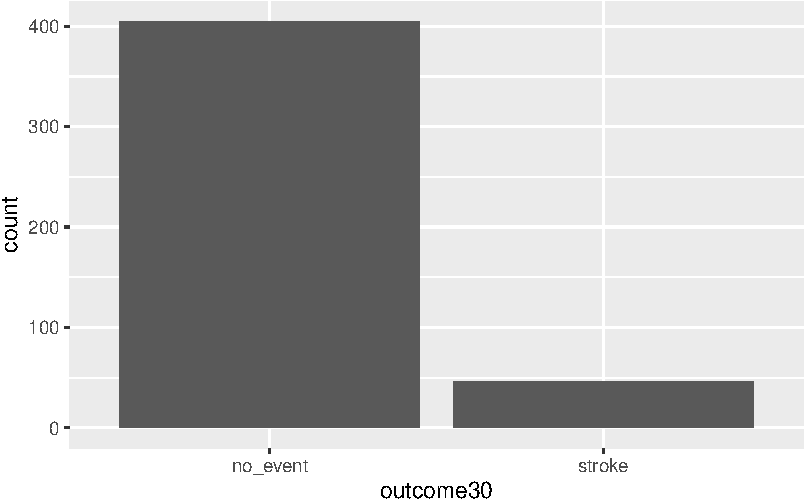
\includegraphics{01-Data-Case-Study_files/figure-pdf/fig-first-1.pdf}

}

\caption{\label{fig-first}Using \textbf{ggformula} to create a bar
chart.}

\end{figure}%

\begin{quote}
\textbf{Exercise}:\\
Explain Figure~\ref{fig-first}.
\end{quote}

This plot graphically shows us the total number of ``stroke'' and the
total number of ``no\_event''. However, this is not what we want. We
want to compare the 30-day outcomes for both treatment groups. So, we
need to break the data into different groups based on treatment type. In
the formula notation, we now update it to the form:

\begin{verbatim}
goal(y ~ x|z, data = MyData, ...) # pseudo-code for the formula template
\end{verbatim}

We read \texttt{y\ \textasciitilde{}\ x\textbar{}z} as ``y tilde x by
z'' and interpret it in the equivalent forms: ``y modeled by x for each
z''; ``y explained by x within each z''; or ``y accounted for by x
within z.'' For graphics, it's reasonable to read the formula as ``y
vs.~x for each z''. Figure Figure~\ref{fig-split} shows the results.

\begin{Shaded}
\begin{Highlighting}[]
\FunctionTok{gf\_bar}\NormalTok{(}\SpecialCharTok{\textasciitilde{}}\NormalTok{outcome30}\SpecialCharTok{|}\NormalTok{group, }\AttributeTok{data =}\NormalTok{ stent\_study) }
\end{Highlighting}
\end{Shaded}

\begin{figure}[H]

\centering{

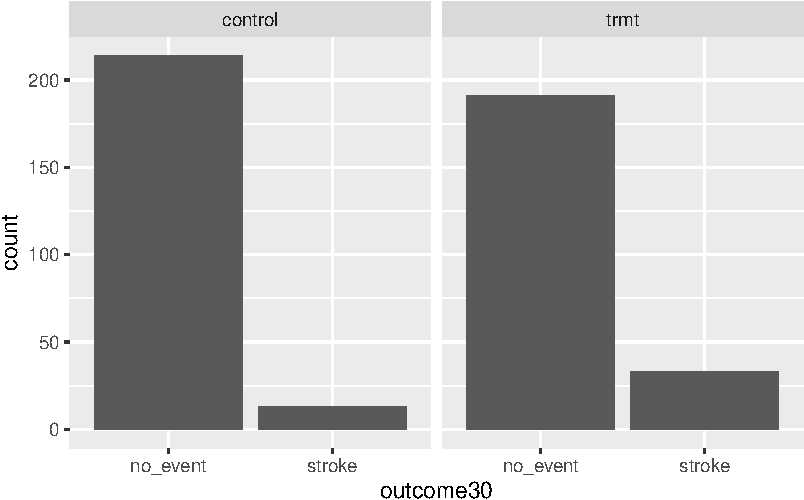
\includegraphics{01-Data-Case-Study_files/figure-pdf/fig-split-1.pdf}

}

\caption{\label{fig-split}Bar charts conditioned on the \texttt{group}
variable.}

\end{figure}%

\subsubsection{More advanced graphics}\label{more-advanced-graphics}

As a prelude for things to come, the above graphic needs work. The
labels don't help and there is no title. We could add color. Does it
make more sense to use proportions? Here is the code and results for a
better graph, see Figure Figure~\ref{fig-cs1}. Don't worry if this seems
a bit advanced, but feel free to examine each new component of this
code.

\begin{Shaded}
\begin{Highlighting}[]
\CommentTok{\# This code creates a graph showing the impact of stents on stroke.}
\CommentTok{\# The \textasciigrave{}gf\_props()\textasciigrave{} function creates a bar graph showing the number of events}
\CommentTok{\# for each experimental group. The \textasciigrave{}fill\textasciigrave{} argument specifies the fill color}
\CommentTok{\# for each group. The \textasciigrave{}position = \textquotesingle{}fill\textquotesingle{}\textasciigrave{} argument specifies that the bars}
\CommentTok{\# should be filled to the top.}

\CommentTok{\# The \textasciigrave{}gf\_labs()\textasciigrave{} function adds the title, subtitle, x{-}axis label, and y{-}axis}
\CommentTok{\# label to the graph.}

\CommentTok{\# The \textasciigrave{}gf\_theme()\textasciigrave{} function applies a black{-}and{-}white theme to the graph.}

\NormalTok{stent\_study }\SpecialCharTok{\%\textgreater{}\%}
\FunctionTok{gf\_props}\NormalTok{(}\SpecialCharTok{\textasciitilde{}}\NormalTok{group, }\AttributeTok{fill =} \SpecialCharTok{\textasciitilde{}}\NormalTok{outcome30, }\AttributeTok{position =} \StringTok{\textquotesingle{}fill\textquotesingle{}}\NormalTok{) }\SpecialCharTok{\%\textgreater{}\%}
  \FunctionTok{gf\_labs}\NormalTok{(}\AttributeTok{title =} \StringTok{"Impact of Stents of Stroke"}\NormalTok{,}
          \AttributeTok{subtitle =} \StringTok{\textquotesingle{}Experiment with 451 Patients\textquotesingle{}}\NormalTok{,}
          \AttributeTok{x =} \StringTok{"Experimental Group"}\NormalTok{,}
          \AttributeTok{y =} \StringTok{"Number of Events"}\NormalTok{) }\SpecialCharTok{\%\textgreater{}\%}
  \FunctionTok{gf\_theme}\NormalTok{(}\FunctionTok{theme\_bw}\NormalTok{())}
\end{Highlighting}
\end{Shaded}

\begin{figure}[H]

\centering{

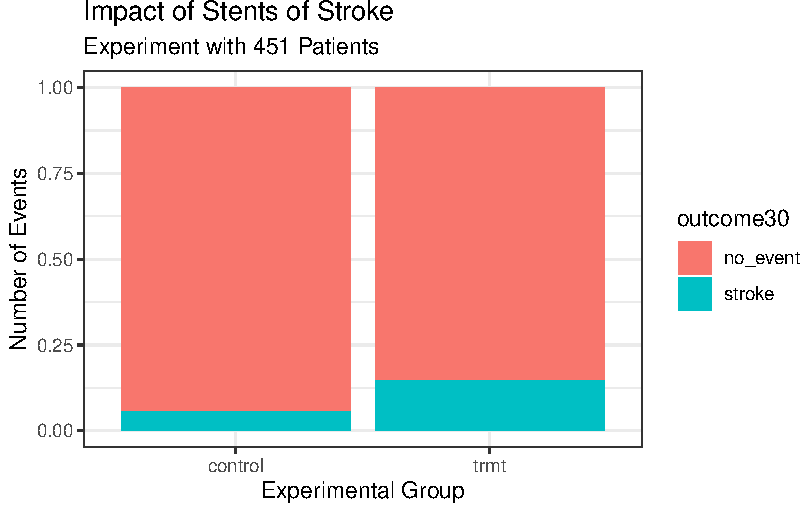
\includegraphics{01-Data-Case-Study_files/figure-pdf/fig-cs1-1.pdf}

}

\caption{\label{fig-cs1}Better graph.}

\end{figure}%

Notice that we used the pipe operator, \texttt{\%\textgreater{}\%}. This
operator allows us to string functions together in a manner that makes
it easier to read the code. In the above code, we are sending the data
object \texttt{stent\_study} into the function \texttt{gf\_props()} to
use as data, so we don't need the \texttt{data\ =} argument. In math,
this is a composition of functions. Instead of \texttt{f(g(x))} we could
use a pipe \texttt{f(g(x))\ =\ g(x)\ \%\textgreater{}\%\ f()}.

\subsection{Conclusion}\label{conclusion}

These two summary statistics (the proportions of people who had a
stroke) are useful in looking for differences in the groups, and we are
in for a surprise: an additional 9\% of patients in the treatment group
had a stroke! This is important for two reasons. First, it is contrary
to what doctors expected, which was that stents would \emph{reduce} the
rate of strokes. Second, it leads to a statistical question: do the data
show a real difference due to the treatment?

This second question is subtle. Suppose you flip a coin 100 times. While
the chance a coin lands heads in any given coin flip is 50\%, we
probably won't observe exactly 50 heads. This type of fluctuation is
part of almost any type of data generating process. It is possible that
the 9\% difference in the stent study is due to this natural variation.
However, the larger the difference we observe (for a particular sample
size), the less believable it is that the difference is due to chance.
So what we are really asking is the following: is the difference so
large that we should reject the notion that it was due to chance?

This is a preview of step 4, analyze the data, and step 5, form a
conclusion, of the analysis cycle. While we haven't yet covered
statistical tools to fully address these steps, we can comprehend the
conclusions of the published analysis: there was compelling evidence of
harm by stents in this study of stroke patients.

\textbf{Be careful:} do not generalize the results of this study to all
patients and all stents. This study looked at patients with very
specific characteristics who volunteered to be a part of this study and
who may not be representative of all stroke patients. In addition, there
are many types of stents and this study only considered the
self-expanding Wingspan stent (Boston Scientific). However, this study
does leave us with an important lesson: we should keep our eyes open for
surprises.

\section{Homework Problems}\label{homework-problems}

Create an Rmd file \texttt{01\ Data\ Case\ Study\ Application.Rmd} in R
(it may be provided), and start by inserting your name in the header.
The code blocks below can be copied and pasted, and then you can
complete the code and answer the questions. When you are done,
\texttt{knit} the Rmd into an html or pdf file by clicking the
\texttt{Knit} button in RStudio and selecting either ``Knit to HTML'' or
``Knit to PDF''.

To create an \texttt{R} code chunk, type CTRL+ALT+I or click the
``Insert a new code chunk'' button (a green C with a + icon) and use the
drop down menu to select \texttt{R}. Anything between the dashes is
interpreted as \texttt{R} code.

For more on RMarkdown, see the following video:
https://www.youtube.com/watch?v=DNS7i2m4sB0. This video only
demonstrates how to \texttt{knit} to an html, but we can also
\texttt{knit} to a pdf since it is set up for us. You can also take the
first chapter of the Data Camp course, \emph{Reporting with R Markdown},
to learn more.

\begin{enumerate}
\def\labelenumi{\arabic{enumi}.}
\tightlist
\item
  \textbf{Stent study continued}. Complete a similar analysis for the
  stent data, but this time use the one year outcome. In particular,
\end{enumerate}

\begin{enumerate}
\def\labelenumi{\alph{enumi}.}
\tightlist
\item
  Read the data into your working directory.
\end{enumerate}

\begin{verbatim}
stent_study <- read_csv(___)
\end{verbatim}

\begin{enumerate}
\def\labelenumi{\alph{enumi}.}
\setcounter{enumi}{1}
\tightlist
\item
  Complete the steps below. The start of code is provided below. You
  will need to add \texttt{\{r\}} to the start of each code chunk or
  insert your own code chunks to use the code.
\end{enumerate}

\begin{verbatim}
i. Use `inspect` on the data.  

inspect(___)

ii. Create a table of `outcome365` and `group`. Comment on the results.  

tally(outcome365 ~ ___, data = stent_study, format = ___, margins = TRUE)

iii. Create a barchart of the data.  

stent_study %>%
  gf_props(~___, fill = ~___, position = 'fill') %>%
  gf_labs(title = ___,
          subtitle = ___,
          x = ___,
          y = ___)
\end{verbatim}

\begin{enumerate}
\def\labelenumi{\arabic{enumi}.}
\setcounter{enumi}{1}
\item
  \textbf{Migraine and acupuncture}. A migraine is a particularly
  painful type of headache, which patients sometimes wish to treat with
  acupuncture. To determine whether acupuncture relieves migraine pain,
  researchers conducted a randomized controlled study where 89 females
  diagnosed with migraine headaches were randomly assigned to one of two
  groups: treatment or control. The 43 patients in the treatment group
  received acupuncture that is specifically designed to treat migraines.
  The 46 patients in the control group received placebo acupuncture
  (needle insertion at nonacupoint locations). Then 24 hours after
  patients received acupuncture, they were asked if they were pain
  free.\footnote{G. Allais et al.~``Ear acupuncture in the treatment of
    migraine attacks: a randomized trial on the efficacy of appropriate
    versus inappropriate acupoints''.
    http://www.ncbi.nlm.nih.gov/pubmed/21533739 In: Neurological Sci.
    32.1 (2011), pp.~173--175.}

  The data is in the file \texttt{migraine\_study.csv} in the
  \texttt{data} folder. Complete the following work:
\end{enumerate}

\begin{enumerate}
\def\labelenumi{\alph{enumi}.}
\tightlist
\item
  Read the data into an object called \texttt{migraine\_study}.
\end{enumerate}

\begin{verbatim}
migraine_study <- read_csv("data/___")

head(migraine_study)
\end{verbatim}

\begin{enumerate}
\def\labelenumi{\alph{enumi}.}
\setcounter{enumi}{1}
\tightlist
\item
  Create a table of the data.
\end{enumerate}

\begin{verbatim}
tally(___)
\end{verbatim}

\begin{enumerate}
\def\labelenumi{\alph{enumi}.}
\setcounter{enumi}{2}
\item
  Report the percent of patients in the treatment group who were pain
  free 24 hours after receiving acupuncture.
\item
  Repeat for the control group.
\item
  At first glance, does acupuncture appear to be an effective treatment
  for migraines? Explain your reasoning.
\item
  Do the data provide convincing evidence that there is a real pain
  reduction for those patients in the treatment group? Or do you think
  that the observed difference might just be due to chance?
\end{enumerate}

\begin{enumerate}
\def\labelenumi{\arabic{enumi}.}
\setcounter{enumi}{2}
\tightlist
\item
  Compile, \texttt{knit}, this report into an html and a pdf. In order
  to \texttt{knit} the report into a pdf, you may need to install the
  \texttt{knitr} and \texttt{tinytex} packages in \texttt{R}.
\end{enumerate}

\section*{\texorpdfstring{\href{https://ds-usafa.github.io/CPS-Solutions-Manual/CS1.html}{Solutions
Manual}}{Solutions Manual}}\label{solutions-manual-1}
\addcontentsline{toc}{section}{\href{https://ds-usafa.github.io/CPS-Solutions-Manual/CS1.html}{Solutions
Manual}}

\markright{Solutions Manual}

\chapter{Data Basics}\label{DB}

\section{Objectives}\label{objectives-2}

\begin{enumerate}
\def\labelenumi{\arabic{enumi})}
\item
  Define and use properly in context all new terminology, to include:
  \emph{case}, \emph{variables}, \emph{data frame}, \emph{associated
  variables}, \emph{independent}, and \emph{discrete} and
  \emph{continuous variables}.
\item
  Identify and define the different types of variables.
\item
  Given a study description, describe the research question.
\item
  In \texttt{R}, create a scatterplot and determine the association of
  two numerical variables from the plot.
\end{enumerate}

\section{Data basics}\label{data-basics-1}

Effective presentation and description of data is a first step in most
analyses. This chapter introduces one structure for organizing data, as
well as some terminology that will be used throughout this book.

\subsection{Observations, variables, and data
matrices}\label{observations-variables-and-data-matrices}

For reference we will be using a data set concerning 50 emails received
in 2012. These observations will be referred to as the \texttt{email50}
data set, and they are a random sample from a larger data set. This data
is in the \textbf{openintro} package so let's install and then load this
package.

\begin{Shaded}
\begin{Highlighting}[]
\FunctionTok{install.packages}\NormalTok{(}\StringTok{"openintro"}\NormalTok{)}
\FunctionTok{library}\NormalTok{(openintro)}
\end{Highlighting}
\end{Shaded}

Table~\ref{tbl-db1} shows 4 rows of the \texttt{email50} data set and we
have elected to only list 5 variables for ease of observation.

Each row in the table represents a single email or
\textbf{case}.\footnote{A case is also sometimes called a \textbf{unit
  of observation} or an \textbf{observational unit}.} The columns
represent \textbf{variables}, which represent characteristics for each
of the cases (emails). For example, the first row represents email 1,
which is not spam, contains 21,705 characters, 551 line breaks, is
written in HTML format, and contains only small numbers.

\begin{longtable}[]{@{}lrrll@{}}

\caption{\label{tbl-db1}First 5 rows of email data frame}

\tabularnewline

\toprule\noalign{}
spam & num\_char & line\_breaks & format & number \\
\midrule\noalign{}
\endhead
\bottomrule\noalign{}
\endlastfoot
0 & 21.705 & 551 & 1 & small \\
0 & 7.011 & 183 & 1 & big \\
1 & 0.631 & 28 & 0 & none \\
0 & 15.829 & 242 & 1 & small \\

\end{longtable}

Let's look at the first 10 rows of data from \texttt{email50} using
\texttt{R}. Remember to ask the two questions:

\emph{What do we want \texttt{R} to do?} and

\emph{What must we give \texttt{R} for it to do this?}

We want the first 10 rows so we use \texttt{head()} and \texttt{R} needs
the data object and the number of rows. The data object is called
\texttt{email50} and is accessible once the \textbf{openintro} package
is loaded.

\begin{Shaded}
\begin{Highlighting}[]
\FunctionTok{head}\NormalTok{(email50, }\AttributeTok{n =} \DecValTok{10}\NormalTok{)}
\end{Highlighting}
\end{Shaded}

\begin{verbatim}
# A tibble: 10 x 21
   spam  to_multiple from     cc sent_email time                image attach
   <fct> <fct>       <fct> <int> <fct>      <dttm>              <dbl>  <dbl>
 1 0     0           1         0 1          2012-01-04 13:19:16     0      0
 2 0     0           1         0 0          2012-02-16 20:10:06     0      0
 3 1     0           1         4 0          2012-01-04 15:36:23     0      2
 4 0     0           1         0 0          2012-01-04 17:49:52     0      0
 5 0     0           1         0 0          2012-01-27 09:34:45     0      0
 6 0     0           1         0 0          2012-01-17 17:31:57     0      0
 7 0     0           1         0 0          2012-03-18 04:18:55     0      0
 8 0     0           1         0 1          2012-03-31 13:58:56     0      0
 9 0     0           1         1 1          2012-01-11 01:57:54     0      0
10 0     0           1         0 0          2012-01-07 19:29:16     0      0
# i 13 more variables: dollar <dbl>, winner <fct>, inherit <dbl>, viagra <dbl>,
#   password <dbl>, num_char <dbl>, line_breaks <int>, format <fct>,
#   re_subj <fct>, exclaim_subj <dbl>, urgent_subj <fct>, exclaim_mess <dbl>,
#   number <fct>
\end{verbatim}

In practice, it is especially important to ask clarifying questions to
ensure important aspects of the data are understood. For instance, it is
always important to be sure we know what each variable means and the
units of measurement. Descriptions of all variables in the
\texttt{email50} data set are given in its documentation which can be
accessed in \texttt{R} by using the \texttt{?} command:

\begin{verbatim}
?email50
\end{verbatim}

(Note that not all data sets will have associated documentation; the
authors of \textbf{openintro} package included this documentation with
the \texttt{email50} data set contained in the package.)

The data in \texttt{email50} represent a \textbf{data matrix}, or in
\texttt{R} terminology a \textbf{data frame} or \textbf{tibble}
\footnote{A tibble is a data frame with attributes for such things as
  better display and printing.}, which is a common way to organize data.
Each row of a data matrix corresponds to a unique case, and each column
corresponds to a variable. This is called \textbf{tidy data}.\footnote{Tidy
  data is data in which each row corresponds to a unique case and each
  column represents a single variable. For more information on tidy
  data, see the \emph{Simply Statistics} blog and the \emph{R for Data
  Science} book by Hadley Wickham and Garrett Grolemund.} The data frame
for the stroke study introduced in the previous chapter had patients as
the cases and there were three variables recorded for each patient. If
we are thinking of patients as the unit of observation, then this data
is tidy.

\begin{verbatim}
# A tibble: 10 x 3
   group   outcome30 outcome365
   <chr>   <chr>     <chr>     
 1 control no_event  no_event  
 2 trmt    no_event  no_event  
 3 control no_event  no_event  
 4 trmt    no_event  no_event  
 5 trmt    no_event  no_event  
 6 control no_event  no_event  
 7 trmt    no_event  no_event  
 8 control no_event  no_event  
 9 control no_event  no_event  
10 control no_event  no_event  
\end{verbatim}

If we think of an outcome as a unit of observation, then it is not tidy
since the two outcome columns are variable values (month or year). The
tidy data for this case would be:

\begin{verbatim}
# A tibble: 10 x 4
   patient_id group   time  result  
        <int> <chr>   <chr> <chr>   
 1          1 control month no_event
 2          1 control year  no_event
 3          2 trmt    month no_event
 4          2 trmt    year  no_event
 5          3 control month no_event
 6          3 control year  no_event
 7          4 trmt    month no_event
 8          4 trmt    year  no_event
 9          5 trmt    month no_event
10          5 trmt    year  no_event
\end{verbatim}

There are three interrelated rules which make a data set tidy:

\begin{enumerate}
\def\labelenumi{\arabic{enumi}.}
\tightlist
\item
  Each variable must have its own column.\\
\item
  Each observation must have its own row.\\
\item
  Each value must have its own cell.
\end{enumerate}

Why ensure that your data is tidy? There are two main advantages:

\begin{enumerate}
\def\labelenumi{\arabic{enumi}.}
\item
  There's a general advantage to picking one consistent way of storing
  data. If you have a consistent data structure, it's easier to learn
  the tools that work with it because they have an underlying
  uniformity.
\item
  There's a specific advantage to placing variables in columns because
  it allows \texttt{R}'s vectorized nature to shine. This will be more
  clear as we progress in our studies. Since most built-in \texttt{R}
  functions work with vectors of values, it makes transforming tidy data
  feel particularly natural.
\end{enumerate}

Data frames are a convenient way to record and store data. If another
individual or case is added to the data set, an additional row can be
easily added. Similarly, another column can be added for a new variable.

\begin{quote}
\textbf{Exercise}:\\
We consider a publicly available data set that summarizes information
about the 3,142 counties in the United States, and we create a data set
called \texttt{county\_subset} data set. This data set will include
information about each county: its name, the state where it resides, its
population in 2000 and 2010, per capita federal spending, poverty rate,
and four additional characteristics. We create this data object in the
code following this description. The parent data set is part of the
\texttt{usdata} library and is called \texttt{county\_complete}. The
variables are summarized in the help menu built into the \textbf{usdata}
package\footnote{\href{http://quickfacts.census.gov/qfd/index.html}{These
  data were collected from the US Census website.}}. How might these
data be organized in a data matrix? \footnote{Each county may be viewed
  as a case, and there are ten pieces of information recorded for each
  case. A table with 3,142 rows and 10 columns could hold these data,
  where each row represents a county and each column represents a
  particular piece of information.}
\end{quote}

Using \texttt{R} we will create our data object. First we load the
library \texttt{usdata}.

\begin{Shaded}
\begin{Highlighting}[]
\FunctionTok{library}\NormalTok{(usdata)}
\end{Highlighting}
\end{Shaded}

We only want a subset of the columns and we will use the \texttt{select}
verb in \texttt{dplyr} to select and rename columns. We also create a
new variable which is federal spending per capita using the
\texttt{mutate} function.

\begin{Shaded}
\begin{Highlighting}[]
\NormalTok{county\_subset }\OtherTok{\textless{}{-}}\NormalTok{ county\_complete }\SpecialCharTok{\%\textgreater{}\%} 
  \FunctionTok{select}\NormalTok{(name, state, pop2000, pop2010, }\AttributeTok{fed\_spend =}\NormalTok{ fed\_spending\_2009, }
         \AttributeTok{poverty =}\NormalTok{ poverty\_2010, }\AttributeTok{homeownership =}\NormalTok{ homeownership\_2010, }
         \AttributeTok{multi\_unit =}\NormalTok{ housing\_multi\_unit\_2010, }\AttributeTok{income =}\NormalTok{ per\_capita\_income\_2010, }
         \AttributeTok{med\_income =}\NormalTok{ median\_household\_income\_2010) }\SpecialCharTok{\%\textgreater{}\%}
  \FunctionTok{mutate}\NormalTok{(}\AttributeTok{fed\_spend =}\NormalTok{ fed\_spend }\SpecialCharTok{/}\NormalTok{ pop2010)}
\end{Highlighting}
\end{Shaded}

Using \texttt{R}, we will display seven rows of the
\texttt{county\_subset} data frame.

\begin{Shaded}
\begin{Highlighting}[]
\FunctionTok{head}\NormalTok{(county\_subset, }\AttributeTok{n =} \DecValTok{7}\NormalTok{)}
\end{Highlighting}
\end{Shaded}

\begin{verbatim}
            name   state pop2000 pop2010 fed_spend poverty homeownership
1 Autauga County Alabama   43671   54571  6.068095    10.6          77.5
2 Baldwin County Alabama  140415  182265  6.139862    12.2          76.7
3 Barbour County Alabama   29038   27457  8.752158    25.0          68.0
4    Bibb County Alabama   20826   22915  7.122016    12.6          82.9
5  Blount County Alabama   51024   57322  5.130910    13.4          82.0
6 Bullock County Alabama   11714   10914  9.973062    25.3          76.9
7  Butler County Alabama   21399   20947  9.311835    25.0          69.0
  multi_unit income med_income
1        7.2  24568      53255
2       22.6  26469      50147
3       11.1  15875      33219
4        6.6  19918      41770
5        3.7  21070      45549
6        9.9  20289      31602
7       13.7  16916      30659
\end{verbatim}

\subsection{Types of variables}\label{types-of-variables}

Examine the \texttt{fed\_spend}, \texttt{pop2010}, and \texttt{state}
variables in the \texttt{county} data set. Each of these variables is
inherently different from the others, yet many of them share certain
characteristics.

First consider \texttt{fed\_spend}. It is said to be a \textbf{numerical
variable} (sometimes called a quantitative variable) since it can take a
wide range of numerical values, and it is sensible to add, subtract, or
take averages with those values. On the other hand, we would not
classify a variable reporting telephone area codes as numerical; even
though area codes are made up of numerical digits, their average, sum,
and difference have no clear meaning.

The \texttt{pop2010} variable is also numerical; it is sensible to add,
subtract, or take averages with those values, although it seems to be a
little different than \texttt{fed\_spend}. This variable of the
population count can only be a whole non-negative number (\(0\), \(1\),
\(2\), \(...\)). For this reason, the population variable is said to be
\textbf{discrete} since it can only take specific numerical values. On
the other hand, the federal spending variable is said to be
\textbf{continuous} because it can take on any value in some interval.
Now technically, there are no truly continuous numerical variables since
all measurements are finite up to some level of accuracy or measurement
precision (e.g., we typically measure federal spending in dollars and
cents). However, in this book, we will treat both types of numerical
variables the same, that is as continuous variables for statistical
modeling. The only place this will be different in this book is in
probability models, which we will see in the probability modeling block.

The variable \texttt{state} can take up to 51 values, after accounting
for Washington, DC, and are summarized as: \emph{Alabama},
\emph{Alaska}, \ldots, and \emph{Wyoming}. Because the responses
themselves are categories, \texttt{state} is a \textbf{categorical
variable} (sometimes also called a qualitative variable), and the
possible values are called the variable's \textbf{levels}.

\begin{figure}

\centering{

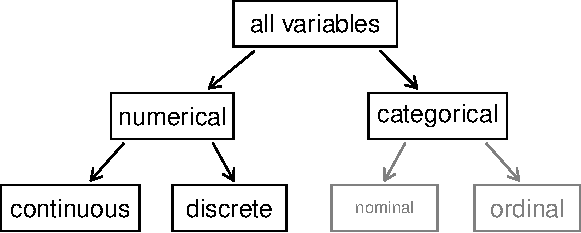
\includegraphics{02-Data-Basics_files/figure-pdf/fig-tax-1.pdf}

}

\caption{\label{fig-tax}Taxonomy of Variables.}

\end{figure}%

Finally, consider a hypothetical variable on education, which describes
the highest level of education completed and takes on one of the values
\emph{noHS}, \emph{HS}, \emph{College} or \emph{Graduate\_school}. This
variable seems to be a hybrid: it is a categorical variable but the
levels have a natural ordering. A variable with these properties is
called an \textbf{ordinal} variable. A categorical variable with levels
that do not have a natural ordering is called a \textbf{nominal}
variable. To simplify analyses, any ordinal variables in this book will
be treated as nominal categorical variables. In \texttt{R}, categorical
variables can be treated in different ways; one of the key differences
is that we can leave them as character values (character strings, or
text) or as factors. A factor is essentially a categorical variable with
defined \emph{levels}. When \texttt{R} handles factors, it is only
concerned about the \emph{levels} of the factors. We will learn more
about this as we progress.

Figure~\ref{fig-tax} captures this classification of variables we have
described.

\begin{quote}
\textbf{Exercise}:\\
Data were collected about students in a statistics course. Three
variables were recorded for each student: number of siblings, student
height, and whether the student had previously taken a statistics
course. Classify each of the variables as continuous numerical, discrete
numerical, or categorical.\footnote{The number of siblings and student
  height represent numerical variables. Because the number of siblings
  is a count, it is discrete. Height varies continuously, so it is a
  continuous numerical variable. The last variable classifies students
  into two categories -- those who have and those who have not taken a
  statistics course -- which makes this variable categorical.}
\end{quote}

\begin{quote}
\textbf{Exercise}:\\
Consider the variables \texttt{group} and \texttt{outcome30} from the
stent study in the case study chapter. Are these numerical or
categorical variables? \footnote{There are only two possible values for
  each variable, and in both cases they describe categories. Thus, each
  is a categorical variable.}
\end{quote}

\subsection{Relationships between
variables}\label{relationships-between-variables}

Many analyses are motivated by a researcher looking for a relationship
between two or more variables. This is the heart of statistical
modeling. A social scientist may like to answer some of the following
questions:

\begin{enumerate}
\def\labelenumi{\arabic{enumi}.}
\tightlist
\item
  Is federal spending, on average, higher or lower in counties with high
  rates of poverty?\\
\item
  If homeownership is lower than the national average in one county,
  will the percent of multi-unit structures in that county likely be
  above or below the national average?
\end{enumerate}

To answer these questions, data must be collected, such as the
\texttt{county\_complete} data set. Examining summary statistics could
provide insights for each of the two questions about counties. Graphs
can be used to visually summarize data and are useful for answering such
questions as well.

Scatterplots are one type of graph used to study the relationship
between two numerical variables. Figure~\ref{fig-pov1} compares the
variables \texttt{fed\_spend} and \texttt{poverty}. Each point on the
plot represents a single county. For instance, the highlighted dot
corresponds to County 1088 in the \texttt{county\_subset} data set:
Owsley County, Kentucky, which had a poverty rate of 41.5\% and federal
spending of \$21.50 per capita. The dense cloud in the scatterplot
suggests a relationship between the two variables: counties with a high
poverty rate also tend to have slightly more federal spending. We might
brainstorm as to why this relationship exists and investigate each idea
to determine which is the most reasonable explanation.

\begin{figure}

\centering{

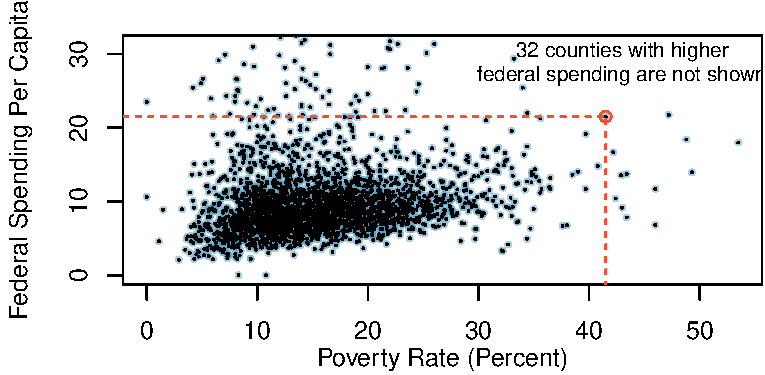
\includegraphics{02-Data-Basics_files/figure-pdf/fig-pov1-1.pdf}

}

\caption{\label{fig-pov1}A scatterplot showing fed\_spend against
poverty. Owsley County of Kentucky, with a poverty rate of 41.5\% and
federal spending of \$21.50 per capita, is highlighted.}

\end{figure}%

\begin{quote}
\textbf{Exercise}:\\
Examine the variables in the \texttt{email50} data set. Create two
research questions about the relationships between these variables that
are of interest to you.\footnote{Two sample questions: (1) Intuition
  suggests that if there are many line breaks in an email then there
  would also tend to be many characters: does this hold true? (2) Is
  there a connection between whether an email format is plain text
  (versus HTML) and whether it is a spam message?}
\end{quote}

The \texttt{fed\_spend} and \texttt{poverty} variables are said to be
associated because the plot shows a discernible pattern. When two
variables show some connection with one another, they are called
\textbf{associated variables}. Associated variables can also be called
\textbf{dependent} variables and vice-versa.

\begin{quote}
\emph{Example}:\\
The relationship between the homeownership rate and the percent of units
in multi-unit structures (e.g.~apartments, condos) is visualized using a
scatterplot in Figure~\ref{fig-homeown}. Are these variables associated?
\end{quote}

It appears that the larger the fraction of units in multi-unit
structures, the lower the homeownership rate. Since there is some
relationship between the variables, they are associated.

\begin{figure}

\centering{

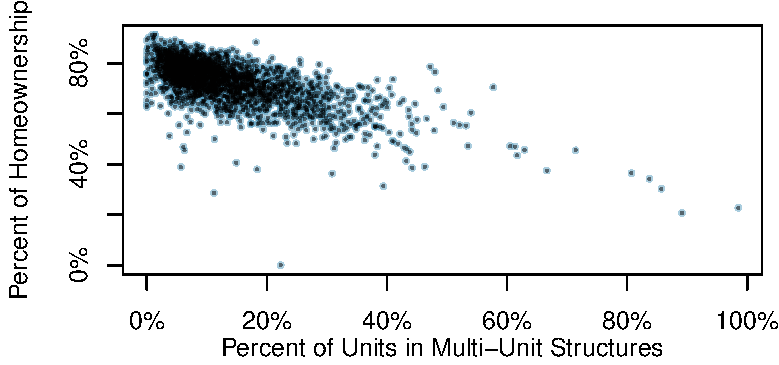
\includegraphics{02-Data-Basics_files/figure-pdf/fig-homeown-1.pdf}

}

\caption{\label{fig-homeown}A scatterplot of the homeownership rate
versus the percent of units that are in multi-unit structures for all
3,143 counties.}

\end{figure}%

Because there is a downward trend in Figure~\ref{fig-homeown} --
counties with more units in multi-unit structures are associated with
lower homeownership -- these variables are said to be \textbf{negatively
associated}. A \textbf{positive association} (upward trend) is shown in
the relationship between the \texttt{poverty} and \texttt{fed\_spend}
variables represented in Figure~\ref{fig-pov1}, where counties with
higher poverty rates tend to receive more federal spending per capita.

If two variables are not associated, then they are said to be
\textbf{independent}. That is, two variables are independent if there is
no evident relationship between the two.

\begin{quote}
A pair of variables are either related in some way (associated) or not
(independent). No pair of variables is both associated and independent.
\end{quote}

\subsection{Creating a scatterplot}\label{creating-a-scatterplot}

In this section, we will create a simple scatterplot and then ask you to
create one on your own. First, we will recreate the scatterplot seen in
Figure~\ref{fig-pov1}. This figure uses the \texttt{county\_subset} data
set.

Here are two questions:

\emph{What do we want \texttt{R} to do?} and

\emph{What must we give \texttt{R} for it to do this?}

We want \texttt{R} to create a scatterplot and to do this it needs, at a
minimum, the data object, what we want on the \(x\)-axis, and what we
want on the \(y\)-axis. More information on
\href{https://cran.r-project.org/web/packages/ggformula/vignettes/ggformula.html}{\textbf{ggformula}}
can be found
\href{https://cran.r-project.org/web/packages/ggformula/vignettes/ggformula-blog.html}{here}.

\begin{Shaded}
\begin{Highlighting}[]
\NormalTok{county\_subset }\SpecialCharTok{\%\textgreater{}\%}
  \FunctionTok{gf\_point}\NormalTok{(fed\_spend }\SpecialCharTok{\textasciitilde{}}\NormalTok{ poverty)}
\end{Highlighting}
\end{Shaded}

\begin{figure}[H]

\centering{

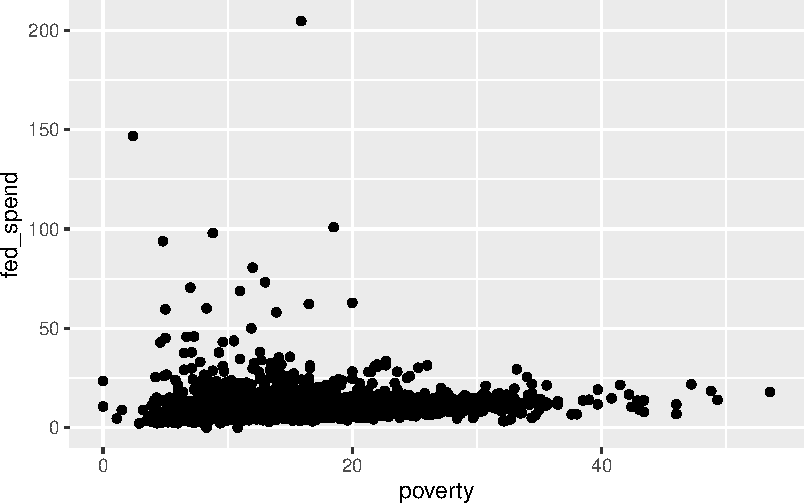
\includegraphics{02-Data-Basics_files/figure-pdf/fig-pov2-1.pdf}

}

\caption{\label{fig-pov2}Scatterplot with \textbf{ggformula}.}

\end{figure}%

Figure~\ref{fig-pov2} is bad. There are poor axis labels, no title,
dense clustering of points, and the \(y\)-axis is being driven by a
couple of extreme points. We will need to clear this up. Again, try to
read the code and use \texttt{help()} or \texttt{?} to determine the
purpose of each command in Figure~\ref{fig-pov3}.

\begin{Shaded}
\begin{Highlighting}[]
\NormalTok{county\_subset }\SpecialCharTok{\%\textgreater{}\%}
  \FunctionTok{filter}\NormalTok{(fed\_spend }\SpecialCharTok{\textless{}} \DecValTok{32}\NormalTok{) }\SpecialCharTok{\%\textgreater{}\%}
  \FunctionTok{gf\_point}\NormalTok{(fed\_spend }\SpecialCharTok{\textasciitilde{}}\NormalTok{ poverty,}
           \AttributeTok{xlab =} \StringTok{"Poverty Rate (Percent)"}\NormalTok{, }
           \AttributeTok{ylab =} \StringTok{"Federal Spending Per Capita"}\NormalTok{,}
           \AttributeTok{title =} \StringTok{"A scatterplot showing fed\_spend against poverty"}\NormalTok{, }
           \AttributeTok{cex =} \DecValTok{1}\NormalTok{, }\AttributeTok{alpha =} \FloatTok{0.2}\NormalTok{) }\SpecialCharTok{\%\textgreater{}\%}
  \FunctionTok{gf\_theme}\NormalTok{(}\FunctionTok{theme\_classic}\NormalTok{())}
\end{Highlighting}
\end{Shaded}

\begin{figure}[H]

\centering{

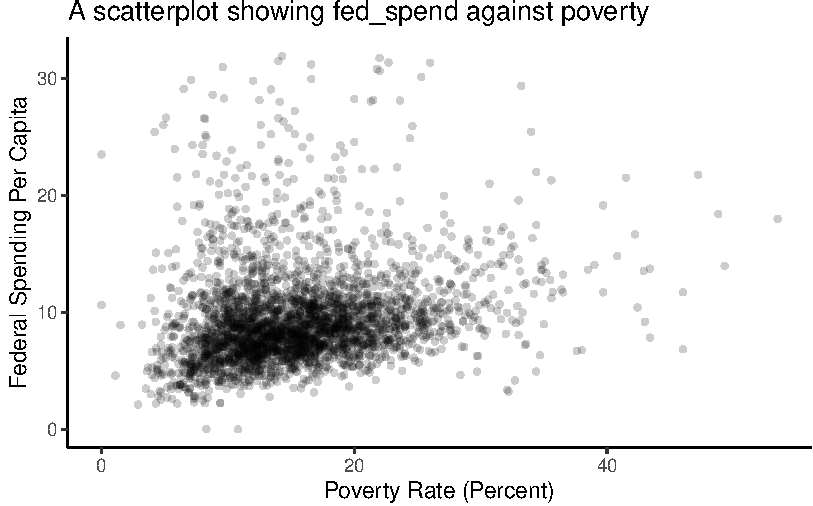
\includegraphics{02-Data-Basics_files/figure-pdf/fig-pov3-1.pdf}

}

\caption{\label{fig-pov3}Better example of a scatterplot.}

\end{figure}%

\begin{quote}
\textbf{Exercise}:\\
Create the scatterplot in Figure~\ref{fig-homeown}.
\end{quote}

\section{Homework Problems}\label{homework-problems-1}

\begin{enumerate}
\def\labelenumi{\arabic{enumi}.}
\tightlist
\item
  \textbf{Identify study components}. Identify (i) the cases, (ii) the
  variables and their types, and (iii) the main research question in the
  studies described below.
\end{enumerate}

\begin{enumerate}
\def\labelenumi{\alph{enumi}.}
\item
  Researchers collected data to examine the relationship between
  pollutants and preterm births in Southern California. During the
  study, air pollution levels were measured by air quality monitoring
  stations. Specifically, levels of carbon monoxide were recorded in
  parts per million, nitrogen dioxide and ozone in parts per hundred
  million, and coarse particulate matter (PM\(_{10}\)) in \(\mu g/m^3\).
  Length of gestation data were collected on 143,196 births between the
  years 1989 and 1993, and air pollution exposure during gestation was
  calculated for each birth. The analysis suggests that increased
  ambient PM\(_{10}\) and, to a lesser degree, CO concentrations may be
  associated with the occurrence of preterm births.\footnote{B. Ritz et
    al.~\href{http://journals.lww.com/epidem/Abstract/2000/09000/Effect_of_Air_Pollution_on_Preterm_Birth_Among.4.aspx}{``Effect
    of air pollution on preterm birth among children born in Southern
    California between 1989 and 1993''}. In: Epidemiology 11.5 (2000),
    pp.~502--511.}
\item
  The Buteyko method is a shallow breathing technique developed by
  Konstantin Buteyko, a Russian doctor, in 1952. Anecdotal evidence
  suggests that the Buteyko method can reduce asthma symptoms and
  improve quality of life. In a scientific study to determine the
  effectiveness of this method, researchers recruited 600 asthma
  patients aged 18-69 who relied on medication for asthma treatment.
  These patients were split into two research groups: patients who
  practiced the Buteyko method and those who did not. Patients were
  scored on quality of life, activity, asthma symptoms, and medication
  reduction on a scale from 0 to 10. On average, the participants in the
  Buteyko group experienced a significant reduction in asthma symptoms
  and an improvement in quality of life.\footnote{J. McGowan. ``Health
    Education: Does the Buteyko Institute Method make a difference?''
    In: Thorax 58 (2003).}
\end{enumerate}

\begin{enumerate}
\def\labelenumi{\arabic{enumi}.}
\setcounter{enumi}{1}
\tightlist
\item
  In the \textbf{openintro} package is a data set called \texttt{ames},
  containing information on individual residential properties sold in
  Ames, IA between 2006 and 2010. Create a scatterplot for the above
  ground living area square feet versus sale price in US dollars.
  Describe the relationship between these two variables. Note: you may
  have to load the library and data set.
\end{enumerate}

\section*{\texorpdfstring{\href{https://ds-usafa.github.io/CPS-Solutions-Manual/DB.html}{Solutions
Manual}}{Solutions Manual}}\label{solutions-manual-2}
\addcontentsline{toc}{section}{\href{https://ds-usafa.github.io/CPS-Solutions-Manual/DB.html}{Solutions
Manual}}

\markright{Solutions Manual}

\chapter{Overview of Data Collection Principles}\label{ODCP}

\section{Objectives}\label{objectives-3}

\begin{enumerate}
\def\labelenumi{\arabic{enumi})}
\item
  Define and use properly in context all new terminology, to include:
  \emph{population}, \emph{sample}, \emph{anecdotal evidence},
  \emph{bias}, \emph{simple random sample}, \emph{systematic sample},
  \emph{non-response bias}, \emph{representative sample},
  \emph{convenience sample}, \emph{explanatory variable}, \emph{response
  variable}, \emph{observational study}, \emph{cohort},
  \emph{experiment}, \emph{randomized experiment}, and \emph{placebo}.
\item
  From a description of a research project, be able to describe the
  population of interest, the generalizability of the study, the
  explanatory and response variables, whether it is observational or
  experimental, and determine the type of sample.
\item
  In the context of a problem, explain how to conduct a sample for the
  different types of sampling procedures.
\end{enumerate}

\section{Overview of data collection
principles}\label{overview-of-data-collection-principles-1}

The first step in conducting research is to identify topics or questions
that are to be investigated. A clearly laid out research question is
helpful in identifying what subjects or cases should be studied and what
variables are important. It is also important to consider \emph{how}
data are collected so that they are reliable and help achieve the
research goals.

\subsection{Populations and samples}\label{populations-and-samples}

Consider the following three research questions:

\begin{enumerate}
\def\labelenumi{\arabic{enumi}.}
\tightlist
\item
  What is the average mercury content in swordfish in the Atlantic
  Ocean?\\
\item
  Over the last 5 years, what is the average time to complete a degree
  for Duke undergraduate students?\\
\item
  Does a new drug reduce the number of deaths in patients with severe
  heart disease?
\end{enumerate}

Each research question refers to a target \textbf{population}, the
entire collection of individuals about which we want information. In the
first question, the target population is all swordfish in the Atlantic
Ocean, and each fish represents a case. It is usually too expensive to
collect data for every case in a population. Instead, a sample is taken.
A \textbf{sample} represents a subset of the cases and is often a small
fraction of the population. For instance, 60 swordfish (or some other
number) in the population might be selected, and this sample data may be
used to provide an estimate of the population average and answer the
research question.

\begin{quote}
\textbf{Exercise}:\\
For the second and third questions above, identify the target population
and what represents an individual case.\footnote{2) Notice that the
  second question is only relevant to students who complete their
  degree; the average cannot be computed using a student who never
  finished her degree. Thus, only Duke undergraduate students who have
  graduated in the last five years represent cases in the population
  under consideration. Each such student would represent an individual
  case. 3) A person with severe heart disease represents a case. The
  population includes all people with severe heart disease.}
\end{quote}

\subsection{Anecdotal evidence}\label{anecdotal-evidence}

Consider the following possible responses to the three research
questions:

\begin{enumerate}
\def\labelenumi{\arabic{enumi}.}
\tightlist
\item
  A man on the news got mercury poisoning from eating swordfish, so the
  average mercury concentration in swordfish must be dangerously high.
\item
  I met two students who took more than 7 years to graduate from Duke,
  so it must take longer to graduate at Duke than at many other
  colleges.
\item
  My friend's dad had a heart attack and died after they gave him a new
  heart disease drug, so the drug must not work.
\end{enumerate}

Each conclusion is based on data. However, there are two problems.
First, the data only represent one or two cases. Second, and more
importantly, it is unclear whether these cases are actually
representative of the population. Data collected in this haphazard
fashion are called \textbf{anecdotal evidence}.

\begin{figure}[H]

{\centering 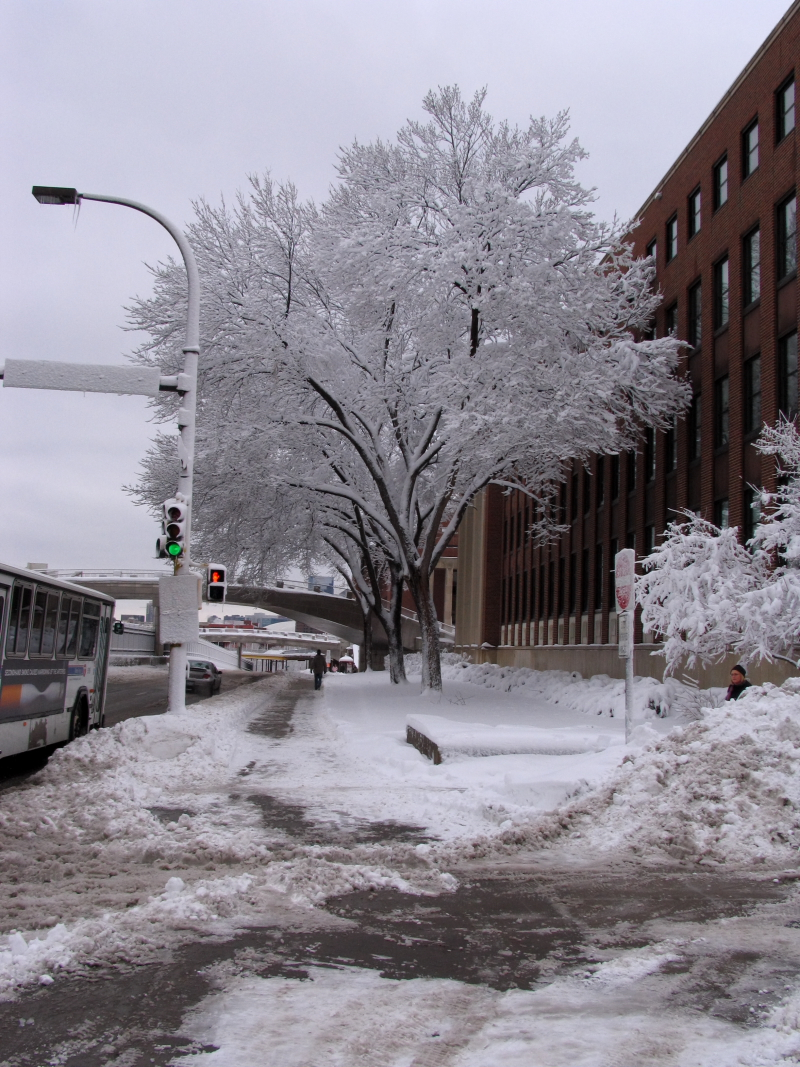
\includegraphics{./figures/mnWinter.JPG}

}

\caption{In February 2010, some media pundits cited one large snow storm
as evidence against global warming. As comedian Jon Stewart pointed out,
\emph{It's one storm, in one region, of one country.}}

\end{figure}%

\begin{quote}
\textbf{Anecdotal evidence}: Be careful of data collected haphazardly.
Such evidence may be true and verifiable, but it may only represent
extraordinary cases.
\end{quote}

Anecdotal evidence typically is composed of unusual cases that we recall
based on their striking characteristics. For instance, we are more
likely to remember the two people we met who took 7 years to graduate
than the six others who graduated in four years. Instead of looking at
the most unusual cases, we should examine a sample of many cases that
represent the population.

\subsection{Sampling from a
population}\label{sampling-from-a-population}

We might try to estimate the time to graduation for Duke undergraduates
in the last 5 years by collecting a sample of students. All graduates in
the last 5 years represent the \emph{population}, and graduates who are
selected for review are collectively called the \emph{sample}. In
general, we always seek to \emph{randomly} select a sample from a
population. The most basic type of random selection is equivalent to how
raffles are conducted. For example, in selecting graduates, we could
write each graduate's name on a raffle ticket and draw 100 tickets. The
selected names would represent a random sample of 100 graduates. This is
illustrated in Figure~\ref{fig-randsamp} .

\begin{figure}

\centering{

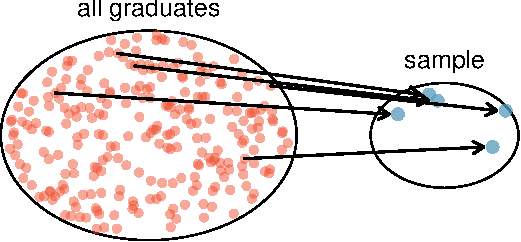
\includegraphics{03-Overview-of-Data-Collection-Principles_files/figure-pdf/fig-randsamp-1.pdf}

}

\caption{\label{fig-randsamp}In this graphic, five graduates are
randomly selected from the population to be included in the sample.}

\end{figure}%

Why pick a sample randomly? Why not just pick a sample by hand? Consider
the following scenario.

\begin{quote}
\textbf{Example}:\\
Suppose we ask a student who happens to be majoring in nutrition to
select several graduates for the study. What kind of students do you
think she might collect? Do you think her sample would be representative
of all graduates? \footnote{Perhaps she would pick a disproportionate
  number of graduates from health-related fields. Or perhaps her
  selection would be well-representative of the population. When
  selecting samples by hand, we run the risk of picking a \emph{biased}
  sample, even if that bias is unintentional or difficult to discern.}
\end{quote}

\begin{figure}

\centering{

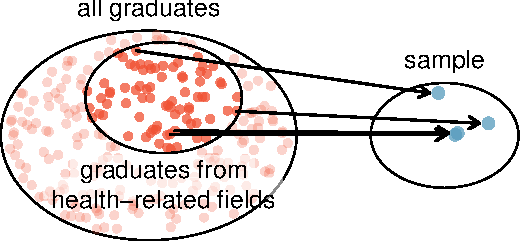
\includegraphics{03-Overview-of-Data-Collection-Principles_files/figure-pdf/fig-biased-1.pdf}

}

\caption{\label{fig-biased}Instead of sampling from all graduates
equally, a nutrition major might inadvertently pick graduates with
health-related majors disproportionately often.}

\end{figure}%

If someone was permitted to pick and choose exactly which graduates were
included in the sample, it is entirely possible that the sample could be
skewed to that person's interests, which may be entirely unintentional.
This introduces \textbf{sampling bias} (see Figure~\ref{fig-biased}),
where some individuals in the population are more likely to be sampled
than others. Sampling randomly helps resolve this problem. The most
basic random sample is called a \textbf{simple random sample}, which is
equivalent to using a raffle to select cases. This means that each case
in the population has an equal chance of being included and there is no
implied connection between the cases in the sample.

Sometimes a simple random sample is difficult to implement and an
alternative method is helpful. One such substitute is a
\textbf{systematic sample}, where one case is sampled after letting a
fixed number of others, say 10 other cases, pass by. Since this approach
uses a mechanism that is not easily subject to personal biases, it often
yields a reasonably representative sample. This book will focus on
simple random samples since the use of systematic samples is uncommon
and requires additional considerations of the context.

The act of taking a simple random sample helps minimize bias. However,
bias can crop up in other ways. Even when people are picked at random,
e.g.~for surveys, caution must be exercised if the non-response is high.
For instance, if only 30\% of the people randomly sampled for a survey
actually respond, and it is unclear whether the respondents are
\textbf{representative}\footnote{A representative sample accurately
  reflects the characteristics of the population.} of the entire
population, the survey might suffer from \textbf{non-response
bias}\footnote{Non-response bias is bias that can be introduced when
  subjects elect not to participate in a study. Often, the individuals
  that do participate are systematically different from the individuals
  who do not.}.

\begin{figure}

\centering{

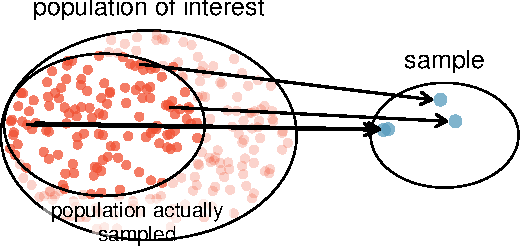
\includegraphics{03-Overview-of-Data-Collection-Principles_files/figure-pdf/fig-convsamp-1.pdf}

}

\caption{\label{fig-convsamp}Due to the possibility of non-response,
surveys studies may only reach a certain group within the population. It
is difficult, and often impossible, to completely fix this problem.}

\end{figure}%

Another common pitfall is a \textbf{convenience sample}, where
individuals who are easily accessible are more likely to be included in
the sample, see Figure~\ref{fig-convsamp}. For instance, if a political
survey is done by stopping people walking in the Bronx, it will not
represent all of New York City. It is often difficult to discern what
sub-population a convenience sample represents.

\begin{quote}
\textbf{Exercise}:\\
We can easily access ratings for products, sellers, and companies
through websites. These ratings are based only on those people who go
out of their way to provide a rating. If 50\% of online reviews for a
product are negative, do you think this means that 50\% of buyers are
dissatisfied with the product?\footnote{Answers will vary. From our own
  anecdotal experiences, we believe people tend to rant more about
  products that fell below expectations than rave about those that
  perform as expected. For this reason, we suspect there is a negative
  bias in product ratings on sites like Amazon. However, since our
  experiences may not be representative, we also keep an open mind.}
\end{quote}

\subsection{Explanatory and response
variables}\label{explanatory-and-response-variables}

Consider the following question for the \texttt{county} data set:

Is federal spending, on average, higher or lower in counties with high
rates of poverty?

If we suspect poverty might affect spending in a county, then poverty is
the \textbf{explanatory} variable and federal spending is the
\textbf{response} variable in the relationship.\footnote{Sometimes the
  explanatory variable is called the \textbf{independent} variable and
  the response variable is called the \textbf{dependent} variable.
  However, this becomes confusing since a \emph{pair} of variables might
  be independent or dependent, so be careful and consider the context
  when using or reading these words.} If there are many variables, it
may be possible to consider a number of them as explanatory variables.

\begin{quote}
\textbf{Explanatory} and \textbf{response} variables\\
To identify the explanatory variable in a pair of variables, identify
which of the two variables is suspected as explaining or causing changes
in the other. In data sets with more than two variables, it is possible
to have multiple explanatory variables. The response variable is the
outcome or result of interest.
\end{quote}

\begin{quote}
\textbf{Caution}: Association does not imply causation. Labeling
variables as \emph{explanatory} and \emph{response} does not guarantee
the relationship between the two is actually causal, even if there is an
association identified between the two variables. We use these labels
only to keep track of which variable we suspect affects the other. We
also use this language to help in our use of \texttt{R} and the formula
notation.
\end{quote}

In some cases, there is no explanatory or response variable. Consider
the following question:

If homeownership in a particular county is lower than the national
average, will the percent of multi-unit structures in that county likely
be above or below the national average?

It is difficult to decide which of these variables should be considered
the explanatory and response variable; i.e.~the direction is ambiguous,
so no explanatory or response labels are suggested here.

\subsection{Introducing observational studies and
experiments}\label{introducing-observational-studies-and-experiments}

There are two primary types of data collection: observational studies
and experiments.

Researchers perform an \textbf{observational study} when they collect
data in a way that does not directly interfere with how the data arise.
For instance, researchers may collect information via surveys, review
medical or company records, or follow a \textbf{cohort}\footnote{A
  cohort is a group of individuals who are similar in some way.} of many
similar individuals to study why certain diseases might develop. In each
of these situations, researchers merely observe what happens. In
general, observational studies can provide evidence of a naturally
occurring association between variables, but by themselves, they cannot
show a causal connection.

When researchers want to investigate the possibility of a causal
connection, they conduct an \textbf{experiment}, a study in which the
explanatory variables are assigned rather than observed. For instance,
we may suspect administering a drug will reduce mortality in heart
attack patients over the following year. To check if there really is a
causal connection between the explanatory variable and the response,
researchers will collect a sample of individuals and split them into
groups. The individuals in each group are \emph{assigned} a treatment.
When individuals are \emph{randomly} assigned to a treatment group, and
we are \emph{comparing} at least two treatments, the experiment is
called a \textbf{randomized comparative experiment}. For example, each
heart attack patient in the drug trial could be randomly assigned,
perhaps by flipping a coin, into one of two groups: the first group
receives a \textbf{placebo} (fake treatment) and the second group
receives the drug. The case study at the beginning of the book is
another example of an experiment, though that study did not employ a
placebo. Math 359 is a course on the design and analysis of experimental
data, DOE, at USAFA. In the Air Force, these types of experiments are an
important part of test and evaluation. Many Air Force analysts are
expert practitioners of DOE. In this book though, we will minimize our
discussion of DOE.

\begin{quote}
\textbf{Association} \(\neq\) Causation\\
Again, association does not imply causation. In a data analysis,
association does not imply causation, and causation can only be inferred
from a randomized experiment. Although, a hot field is the analysis of
causal relationships in observational data. This is important because
consider cigarette smoking, how do we know it causes lung cancer? We
only have observational data and clearly cannot do an experiment. We
think analysts will be charged in the near future with using causal
reasoning on observational data.
\end{quote}

\section{Homework Problems}\label{homework-problems-2}

\begin{enumerate}
\def\labelenumi{\arabic{enumi}.}
\tightlist
\item
  \textbf{Generalizability and causality}. Identify the population of
  interest and the sample in the studies described below. These are the
  same studies from the previous chapter. Also comment on whether or not
  the results of the study can be generalized to the population and if
  the findings of the study can be used to establish causal
  relationships.
\end{enumerate}

\begin{enumerate}
\def\labelenumi{\alph{enumi}.}
\item
  Researchers collected data to examine the relationship between
  pollutants and preterm births in Southern California. During the
  study, air pollution levels were measured by air quality monitoring
  stations. Specifically, levels of carbon monoxide were recorded in
  parts per million, nitrogen dioxide and ozone in parts per hundred
  million, and coarse particulate matter (PM\(_{10}\)) in \(\mu g/m^3\).
  Length of gestation data were collected on 143,196 births between the
  years 1989 and 1993, and air pollution exposure during gestation was
  calculated for each birth. The analysis suggests that increased
  ambient PM\(_{10}\) and, to a lesser degree, CO concentrations may be
  associated with the occurrence of preterm births.\footnote{B. Ritz et
    al.~\href{http://journals.lww.com/epidem/Abstract/2000/09000/Effect_of_Air_Pollution_on_Preterm_Birth_Among.4.aspx}{``Effect
    of air pollution on preterm birth among children born in Southern
    California between 1989 and 1993''}. In: Epidemiology 11.5 (2000),
    pp.~502--511.}
\item
  The Buteyko method is a shallow breathing technique developed by
  Konstantin Buteyko, a Russian doctor, in 1952. Anecdotal evidence
  suggests that the Buteyko method can reduce asthma symptoms and
  improve quality of life. In a scientific study to determine the
  effectiveness of this method, researchers recruited 600 asthma
  patients aged 18-69 who relied on medication for asthma treatment.
  These patients were split into two research groups: patients who
  practiced the Buteyko method and those who did not. Patients were
  scored on quality of life, activity, asthma symptoms, and medication
  reduction on a scale from 0 to 10. On average, the participants in the
  Buteyko group experienced a significant reduction in asthma symptoms
  and an improvement in quality of life.\footnote{J. McGowan. ``Health
    Education: Does the Buteyko Institute Method make a difference?''
    In: Thorax 58 (2003).}
\end{enumerate}

\begin{enumerate}
\def\labelenumi{\arabic{enumi}.}
\setcounter{enumi}{1}
\tightlist
\item
  \textbf{GPA and study time}. A survey was conducted on 193
  undergraduates who took an introductory statistics course at a private
  US university in 2012. This survey asked them about their GPA and the
  number of hours they spent studying per week. The scatterplot below
  displays the relationship between these two variables.
\end{enumerate}

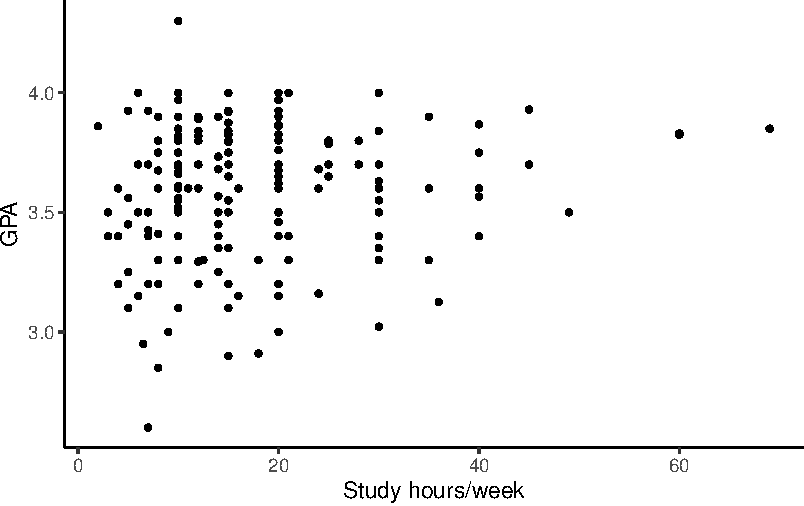
\includegraphics{03-Overview-of-Data-Collection-Principles_files/figure-pdf/unnamed-chunk-6-1.pdf}

\begin{enumerate}
\def\labelenumi{\alph{enumi}.}
\item
  What is the explanatory variable and what is the response variable?
\item
  Describe the relationship between the two variables. Make sure to
  discuss unusual observations, if any.
\item
  Is this an experiment or an observational study?
\item
  Can we conclude that studying longer hours leads to higher GPAs?
\end{enumerate}

\begin{enumerate}
\def\labelenumi{\arabic{enumi}.}
\setcounter{enumi}{2}
\tightlist
\item
  \textbf{Income and education} The scatterplot below shows the
  relationship between per capita income (in thousands of dollars) and
  percent of population with a bachelor's degree in 3,143 counties in
  the US in 2010.
\end{enumerate}

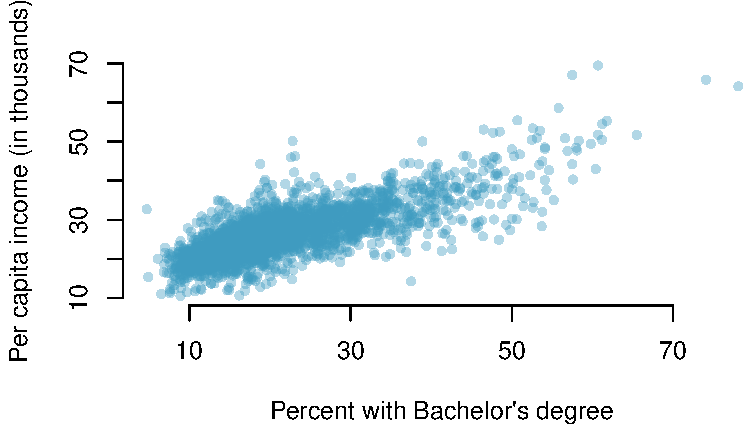
\includegraphics{03-Overview-of-Data-Collection-Principles_files/figure-pdf/unnamed-chunk-7-1.pdf}

\begin{enumerate}
\def\labelenumi{\alph{enumi}.}
\item
  What are the explanatory and response variables?
\item
  Describe the relationship between the two variables. Make sure to
  discuss unusual observations, if any.
\item
  Can we conclude that having a bachelor's degree increases one's
  income?
\end{enumerate}

\section*{\texorpdfstring{\href{https://ds-usafa.github.io/CPS-Solutions-Manual/ODCP.html}{Solutions
Manual}}{Solutions Manual}}\label{solutions-manual-3}
\addcontentsline{toc}{section}{\href{https://ds-usafa.github.io/CPS-Solutions-Manual/ODCP.html}{Solutions
Manual}}

\markright{Solutions Manual}

\chapter{Studies}\label{STUDY}

\section{Objectives}\label{objectives-4}

\begin{enumerate}
\def\labelenumi{\arabic{enumi})}
\item
  Define and use properly in context all new terminology, to include:
  \emph{confounding variable}, \emph{prospective study},
  \emph{retrospective study}, \emph{simple random sampling},
  \emph{stratified sampling}, \emph{strata}, \emph{cluster sampling},
  \emph{multistage sampling}, \emph{experiment}, \emph{randomized
  experiment}, \emph{control}, \emph{replicate}, \emph{blocking},
  \emph{blocks}, \emph{treatment group}, \emph{control group},
  \emph{blinded study}, \emph{placebo}, \emph{placebo effect}, and
  \emph{double-blind}.
\item
  Given a study description, be able to describe the study using correct
  terminology.
\item
  Given a scenario, describe flaws in reasoning and propose study and
  sampling designs.
\end{enumerate}

\section{Observation studies, sampling strategies, and
experiments}\label{observation-studies-sampling-strategies-and-experiments}

\subsection{Observational studies}\label{observational-studies}

Generally, data in observational studies are collected only by
monitoring what occurs, while experiments require the primary
explanatory variable in a study be assigned for each subject by the
researchers.

Making causal conclusions based on experiments is often reasonable.
However, making the same causal conclusions based on observational data
can be treacherous and is not recommended. Thus, observational studies
are generally only sufficient to show associations.

\begin{quote}
\textbf{Exercise}:\\
Suppose an observational study tracked sunscreen use and skin cancer,
and it was found that the more sunscreen someone used, the more likely
the person was to have skin cancer. Does this mean sunscreen
\emph{causes} skin cancer?\footnote{No.~See the paragraph following the
  exercise for an explanation.}
\end{quote}

Some previous research\footnote{http://www.sciencedirect.com/science/article/pii/S0140673698121682\\
  http://archderm.ama-assn.org/cgi/content/abstract/122/5/537\\
  Study with a similar scenario to that described here:\\
  http://onlinelibrary.wiley.com/doi/10.1002/ijc.22745/full} tells us
that using sunscreen actually reduces skin cancer risk, so maybe there
is another variable that can explain this hypothetical association
between sunscreen usage and skin cancer. One important piece of
information that is absent is sun exposure. If someone is out in the sun
all day, she is more likely to use sunscreen \emph{and} more likely to
get skin cancer. Exposure to the sun is unaccounted for in the simple
investigation.

\begin{figure}

\centering{

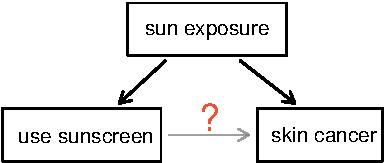
\includegraphics{04-Studies_files/figure-pdf/fig-confound-1.pdf}

}

\caption{\label{fig-confound}un exposure is a confounding variable
because it is related to both response and explanatory variables.}

\end{figure}%

Sun exposure is what is called a \textbf{confounding
variable},\footnote{Also called a \textbf{lurking variable},
  \textbf{confounding factor}, or a \textbf{confounder}.} which is a
variable that is correlated with both the explanatory and response
variables, see Figure~\ref{fig-confound}. While one method to justify
making causal conclusions from observational studies is to exhaust the
search for confounding variables, there is no guarantee that all
confounding variables can be examined or measured.

Let's look at an example of confounding visually. Using the \texttt{SAT}
data from the \textbf{mosaic} package let's look at expenditure per
pupil versus SAT scores. Figure~\ref{fig-confound2} is a plot of the
data.

\begin{quote}
\textbf{Exercise}:\\
What conclusion do you reach from the plot in
Figure~\ref{fig-confound2}?\footnote{It appears that average SAT score
  declines as expenditures per student increases.}
\end{quote}

\begin{figure}

\centering{

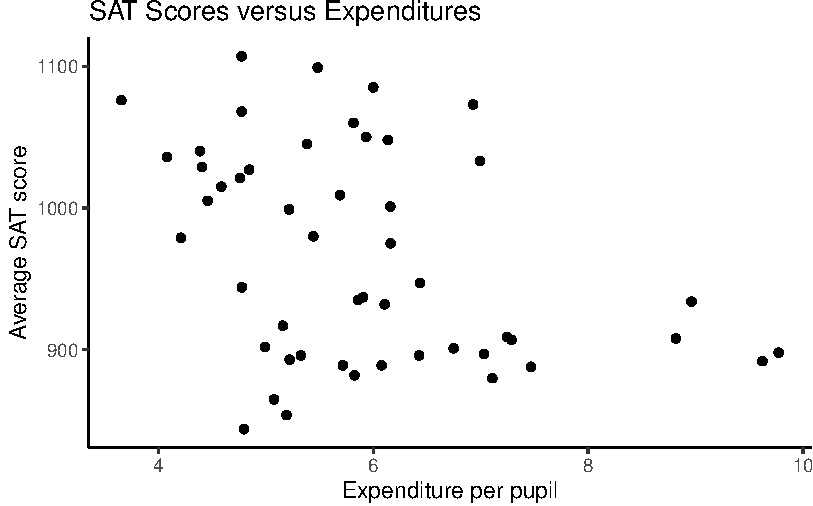
\includegraphics{04-Studies_files/figure-pdf/fig-confound2-1.pdf}

}

\caption{\label{fig-confound2}Average SAT score versus expenditure per
pupil; reminder: each observation represents an individual state.}

\end{figure}%

The implication that spending less might give better results is not
justified. Expenditures are confounded with the proportion of students
who take the exam, and scores are higher in states where fewer students
take the exam.

It is interesting to look at the original plot if we place the states
into two groups depending on whether more or fewer than 40\% of students
take the SAT. Figure~\ref{fig-conditional} is a plot of the data broken
down into the 2 groups.

\begin{figure}

\centering{

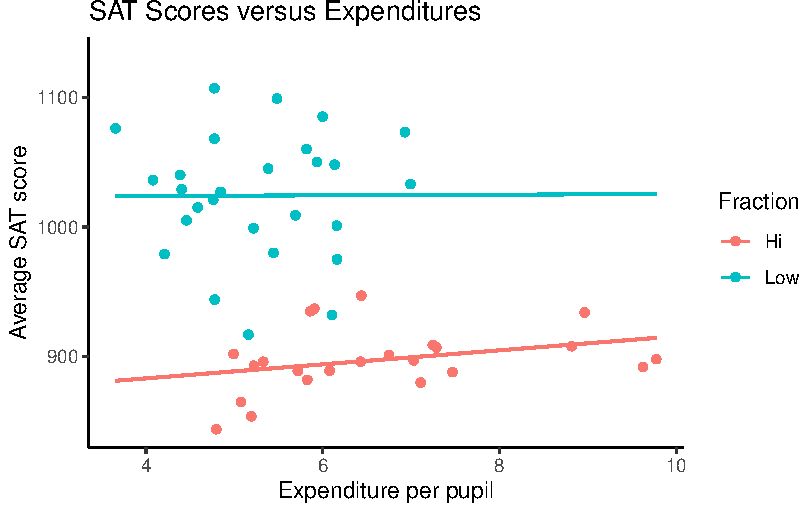
\includegraphics{04-Studies_files/figure-pdf/fig-conditional-1.pdf}

}

\caption{\label{fig-conditional}Average SAT score versus expenditure per
pupil; broken down by level of participation.}

\end{figure}%

Once we account for the fraction of students taking the SAT, the
relationship between expenditures and SAT scores changes.

In the same way, the \texttt{county} data set is an observational study
with confounding variables, and its data cannot easily be used to make
causal conclusions.

\begin{quote}
\textbf{Exercise}:\\
Figure~\ref{fig-homeown2} shows a negative association between the
homeownership rate and the percentage of multi-unit structures in a
county. However, it is unreasonable to conclude that there is a causal
relationship between the two variables. Suggest one or more other
variables that might explain the relationship in the
Figure~\ref{fig-homeown2}.\footnote{Answers will vary. Population
  density may be important. If a county is very dense, then a larger
  fraction of residents may live in multi-unit structures. Additionally,
  the high density may contribute to increases in property value, making
  homeownership infeasible for many residents.}
\end{quote}

\begin{figure}

\centering{

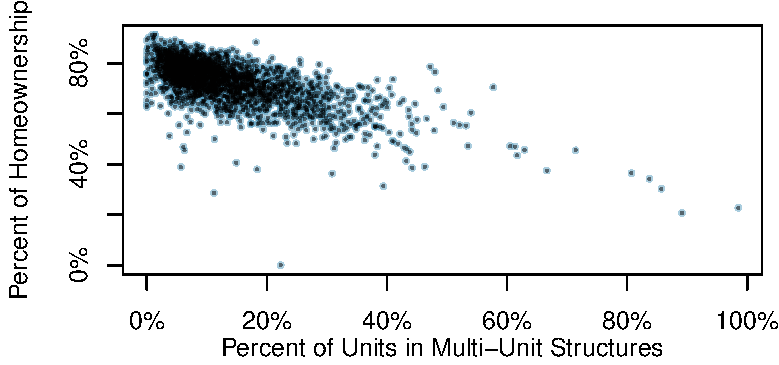
\includegraphics{04-Studies_files/figure-pdf/fig-homeown2-1.pdf}

}

\caption{\label{fig-homeown2}A scatterplot of the homeownership rate
versus the percent of units that are in multi-unit structures for all
3,143 counties.}

\end{figure}%

Observational studies come in two forms: prospective and retrospective
studies. A \textbf{prospective study} identifies individuals and
collects information as events unfold. For instance, medical researchers
may identify and follow a group of similar individuals over many years
to assess the possible influences of behavior on cancer risk. One
example of such a study is The Nurses Health Study, started in 1976 and
expanded in 1989.\footnote{http://www.channing.harvard.edu/nhs/} This
prospective study recruits registered nurses and then collects data from
them using questionnaires.

\textbf{Retrospective studies} collect data after events have taken
place; e.g.~researchers may review past events in medical records. Some
data sets, such as \texttt{county}, may contain both prospectively- and
retrospectively-collected variables. Local governments prospectively
collect some variables as events unfolded (e.g.~retail sales) while the
federal government retrospectively collected others during the 2010
census (e.g.~county population).

\subsection{Three sampling methods}\label{three-sampling-methods}

Almost all statistical methods are based on the notion of implied
randomness. If observational data are not collected in a random
framework from a population, results from these statistical methods are
not reliable. Here we consider three random sampling techniques: simple,
stratified, and cluster sampling. Figure~\ref{fig-simprand},
Figure~\ref{fig-stratsamp2}, and Figure~\ref{fig-clussamp4} provide a
graphical representation of these techniques.

\begin{figure}

\centering{

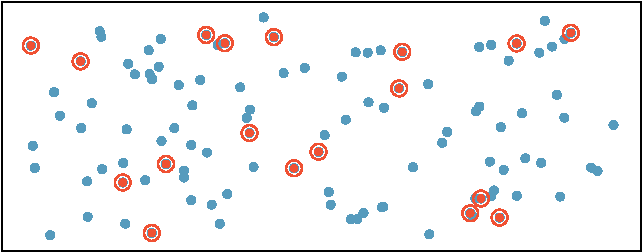
\includegraphics{04-Studies_files/figure-pdf/fig-simprand-1.pdf}

}

\caption{\label{fig-simprand}Examples of simple random sampling. In this
figure, simple random sampling was used to randomly select the 18
cases.}

\end{figure}%

\begin{figure}

\centering{

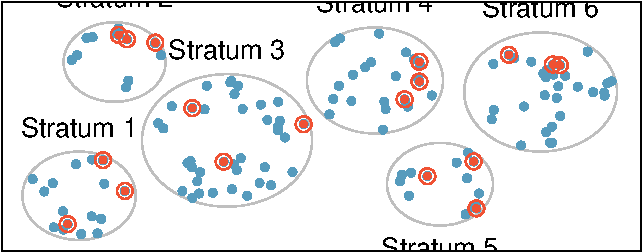
\includegraphics{04-Studies_files/figure-pdf/fig-stratsamp2-1.pdf}

}

\caption{\label{fig-stratsamp2}In this figure, stratified sampling was
used: cases were grouped into strata, and then simple random sampling
was employed within each stratum.}

\end{figure}%

\begin{figure}

\centering{

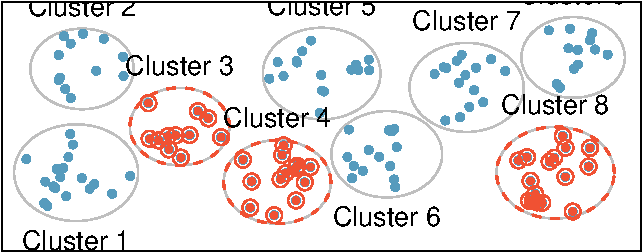
\includegraphics{04-Studies_files/figure-pdf/fig-clussamp4-1.pdf}

}

\caption{\label{fig-clussamp4}In this figure, cluster sampling was used,
where data were binned into nine clusters, and three of the clusters
were randomly selected.}

\end{figure}%

\textbf{Simple random sampling} is probably the most intuitive form of
random sampling, in which each individual in the population has an equal
chance of being chosen. Consider the salaries of Major League Baseball
(MLB) players, where each player is a member of one of the league's 30
teams. To take a simple random sample of 120 baseball players and their
salaries from the 2010 season, we could write the names of that season's
828 players onto slips of paper, drop the slips into a bucket, shake the
bucket around until we are sure the names are all mixed up, then draw
out slips until we have the sample of 120 players. In general, a sample
is referred to as ``simple random'' if each case in the population has
an equal chance of being included in the final sample \emph{and} knowing
that a case is included in a sample does not provide useful information
about which other cases are included or not.

\textbf{Stratified sampling} is a divide-and-conquer sampling strategy.
The population is divided into groups called \textbf{strata}. The strata
are chosen so that similar cases are grouped together, then a second
sampling method, usually simple random sampling, is employed within each
stratum. In the baseball salary example, the teams could represent the
strata; some teams have a lot more money (we're looking at you,
Yankees). Then we might randomly sample 4 players from each team for a
total of 120 players.

Stratified sampling is especially useful when the cases in each stratum
are very similar with respect to the outcome of interest. The downside
is that analyzing data from a stratified sample is a more complex task
than analyzing data from a simple random sample. The analysis methods
introduced in this book would need to be extended to analyze data
collected using stratified sampling.

\begin{quote}
\textbf{Example}:\\
Why would it be good for cases within each stratum to be very
similar?\footnote{We might get a more stable estimate for the
  subpopulation in a stratum if the cases are very similar. These
  improved estimates for each subpopulation will help us build a
  reliable estimate for the full population.}
\end{quote}

In \textbf{cluster sampling}, we group observations into clusters, then
randomly sample some of the clusters. Sometimes cluster sampling can be
a more economical technique than the alternatives. Also, unlike
stratified sampling, cluster sampling is most helpful when there is a
lot of case-to-case variability within a cluster but the clusters
themselves don't look very different from one another. For example, if
neighborhoods represented clusters, then this sampling method works best
when the neighborhoods are very diverse. A downside of cluster sampling
is that more advanced analysis techniques are typically required, though
the methods in this book can be extended to handle such data.

\begin{quote}
\textbf{Example}:\\
Suppose we are interested in estimating the malaria rate in a densely
tropical portion of rural Indonesia. We learn that there are 30 villages
in that part of the Indonesian jungle, each more or less similar to the
next. What sampling method should be employed?\footnote{A simple random
  sample would likely draw individuals from all 30 villages, which could
  make data collection extremely expensive. Stratified sampling would be
  a challenge since it is unclear how we would build strata of similar
  individuals. However, cluster sampling seems like a very good idea. We
  might randomly select a small number of villages. This would probably
  reduce our data collection costs substantially in comparison to a
  simple random sample and would still give us helpful information.}
\end{quote}

Another technique called \textbf{multistage sampling} is similar to
cluster sampling, except that we take a simple random sample within each
selected cluster. For instance, if we sampled neighborhoods using
cluster sampling, we would next sample a subset of homes within each
selected neighborhood if we were using multistage sampling.

\subsection{Experiments}\label{experiments}

Studies where the researchers assign treatments to cases are called
\textbf{experiments}. When this assignment includes randomization,
e.g.~using a coin flip to decide which treatment a patient receives, it
is called a \textbf{randomized experiment}. Randomized experiments are
fundamentally important when trying to show a causal connection between
two variables.

\subsubsection{Principles of experimental
design}\label{principles-of-experimental-design}

Randomized experiments are generally built on four principles.

\begin{enumerate}
\def\labelenumi{\arabic{enumi}.}
\item
  \textbf{Controlling}. Researchers assign treatments to cases, and they
  do their best to \textbf{control} any other differences in the groups.
  For example, when patients take a drug in pill form, some patients
  take the pill with only a sip of water while others may have it with
  an entire glass of water. To control for the effect of water
  consumption, a doctor may ask all patients to drink a 12 ounce glass
  of water with the pill.
\item
  \textbf{Randomization}. Researchers randomize patients into treatment
  groups to account for variables that cannot be controlled. For
  example, some patients may be more susceptible to a disease than
  others due to their dietary habits. Randomizing patients into the
  treatment or control group helps even out such differences, and it
  also prevents accidental bias from entering the study.
\item
  \textbf{Replication}. The more cases researchers observe, the more
  accurately they can estimate the effect of the explanatory variable on
  the response. In a single study, we \textbf{replicate} by collecting a
  sufficiently large sample. Additionally, a group of scientists may
  replicate an entire study to verify an earlier finding. You replicate
  to the level of variability you want to estimate. For example, in
  flight test, we can run the same flight conditions again to get a
  replicate; however, if the same plane and pilot are being used, the
  replicate is not getting the pilot-to-pilot or the plane-to-plane
  variability.
\item
  \textbf{Blocking}. Researchers sometimes know or suspect that
  variables, other than the treatment, influence the response. Under
  these circumstances, they may first group individuals based on this
  variable and then randomize cases within each block, or group, to the
  treatments. This strategy is often referred to as \textbf{blocking}.
  For instance, if we are looking at the effect of a drug on heart
  attacks, we might first split patients into low-risk and high-risk
  blocks, then randomly assign half the patients from each block to the
  control group and the other half to the treatment group, as shown in
  Figure~\ref{fig-exp4}. This strategy ensures each treatment group has
  an equal number of low-risk and high-risk patients.
\end{enumerate}

\begin{figure}

\centering{

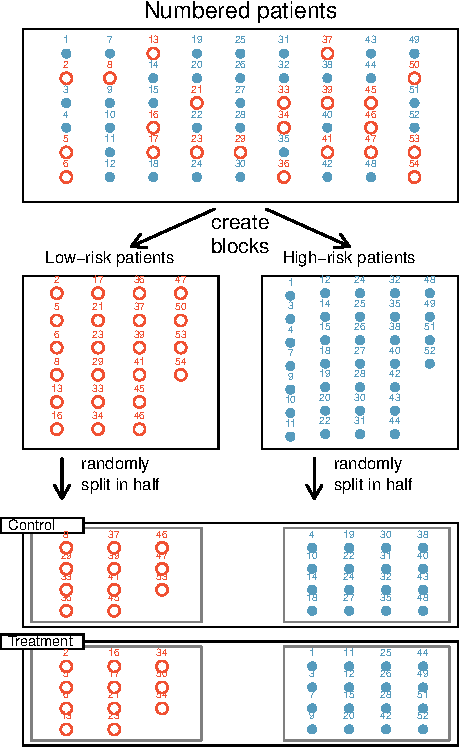
\includegraphics{04-Studies_files/figure-pdf/fig-exp4-1.pdf}

}

\caption{\label{fig-exp4}Blocking using a variable depicting patient
risk. Patients are first divided into low-risk and high-risk blocks,
then each block is evenly divided into the treatment groups using
randomization. This strategy ensures an equal representation of patients
in each treatment group from both the low-risk and high-risk
categories.}

\end{figure}%

It is important to incorporate the first three experimental design
principles into any study, and this chapter describes methods for
analyzing data from such experiments. Blocking is a slightly more
advanced technique, and statistical methods in this chapter may be
extended to analyze data collected using blocking. Math 359 is an entire
course at USAFA devoted to the design and analysis of experiments.

\subsubsection{Reducing bias in human
experiments}\label{reducing-bias-in-human-experiments}

Randomized experiments are the gold standard for data collection, but
they do not ensure an unbiased perspective into the cause and effect
relationships in all cases. Human studies are perfect examples where
bias can unintentionally arise. Here we reconsider a study where a new
drug was used to treat heart attack patients.\footnote{Anturane
  Reinfarction Trial Research Group. 1980. Sulfinpyrazone in the
  prevention of sudden death after myocardial infarction. New England
  Journal of Medicine 302(5):250-256.} In particular, researchers wanted
to know if the drug reduced deaths in patients.

These researchers designed a randomized experiment because they wanted
to draw causal conclusions about the drug's effect. Study
volunteers\footnote{Human subjects are often called \textbf{patients},
  \textbf{volunteers}, or \textbf{study participants}.} were randomly
placed into two study groups. One group, the \textbf{treatment group},
received the experimental treatment of interest (the new drug to treat
heart attack patients). The other group, called the \textbf{control
group}, did not receive any drug treatment. The comparison between the
treatment and control groups allows researchers to determine whether the
treatment really has an effect.

Put yourself in the place of a person in the study. If you are in the
treatment group, you are given a fancy new drug that you anticipate will
help you. On the other hand, a person in the other group doesn't receive
the drug and sits idly, hoping her participation doesn't increase her
risk of death. These perspectives suggest there are actually two
effects: the one of interest is the effectiveness of the drug, and the
second is an emotional effect that is difficult to quantify.

Researchers aren't usually interested in the emotional effect, which
might bias the study. To circumvent this problem, researchers do not
want patients to know which group they are in. When researchers keep the
patients uninformed about their treatment, the study is said to be
\textbf{blind}. But there is one problem: if a patient doesn't receive a
treatment, she will know she is in the control group. The solution to
this problem is to give fake treatments to patients in the control
group. A fake treatment is called a \textbf{placebo}, and an effective
placebo is the key to making a study truly blind. A classic example of a
placebo is a sugar pill that is made to look like the actual treatment
pill. Often times, a placebo results in a slight but real improvement in
patients. This effect has been dubbed the \textbf{placebo effect}.

The patients are not the only ones who should be blinded: doctors and
researchers can accidentally bias a study. When a doctor knows a patient
has been given the real treatment, she might inadvertently give that
patient more attention or care than a patient that she knows is on the
placebo. To guard against this bias, which again has been found to have
a measurable effect in some instances, most modern studies employ a
\textbf{double-blind} setup where doctors or researchers who interact
with patients are, just like the patients, unaware of who is or is not
receiving the treatment.\footnote{There are always some researchers in
  the study who do know which patients are receiving which treatment.
  However, they do not interact with the study's patients and do not
  tell the blinded health care professionals who is receiving which
  treatment.}

\begin{quote}
\textbf{Exercise}:\\
Look back to the stent study in the first chapter where researchers were
testing whether stents were effective at reducing strokes in at-risk
patients. Is this an experiment? Was the study blinded? Was it
double-blinded?\footnote{The researchers assigned the patients into
  their treatment groups, so this study was an experiment. However, the
  patients could distinguish what treatment they received, so this study
  was not blind. The study could not be double-blind since it was not
  blind.}
\end{quote}

\section{Homework Problems}\label{homework-problems-3}

\begin{enumerate}
\def\labelenumi{\arabic{enumi}.}
\tightlist
\item
  \textbf{Propose a sampling strategy}. A large college class has 160
  students. All 160 students attend the lectures together, but the
  students are divided into 4 groups, each with 40 students, for lab
  sections administered by different teaching assistants. The professor
  wants to conduct a survey about how satisfied the students are with
  the course, and he believes that the lab section a student is in might
  affect the student's overall satisfaction with the course.
\end{enumerate}

\begin{enumerate}
\def\labelenumi{\alph{enumi}.}
\item
  What type of study is this?
\item
  Suggest a sampling strategy for carrying out this study.
\end{enumerate}

\begin{enumerate}
\def\labelenumi{\arabic{enumi}.}
\setcounter{enumi}{1}
\tightlist
\item
  \textbf{Flawed reasoning}. Identify the flaw in reasoning in the
  following scenarios. Explain what the individuals in the study should
  have done differently if they want to be able to make such strong
  conclusions.
\end{enumerate}

\begin{enumerate}
\def\labelenumi{\alph{enumi}.}
\item
  Students at an elementary school are given a questionnaire that they
  are required to return after their parents have completed it. One of
  the questions asked is, \emph{Do you find that your work schedule
  makes it difficult for you to spend time with your kids after school?}
  Of the parents who replied, 85\% said \emph{no}. Based on these
  results, the school officials conclude that a great majority of the
  parents have no difficulty spending time with their kids after school.
\item
  A survey is conducted on a simple random sample of 1,000 women who
  recently gave birth, asking them about whether or not they smoked
  during pregnancy. A follow-up survey asking if the children have
  respiratory problems is conducted 3 years later, however, only 567 of
  these women are reached at the same address. The researcher reports
  that these 567 women are representative of all mothers.
\end{enumerate}

\begin{enumerate}
\def\labelenumi{\arabic{enumi}.}
\setcounter{enumi}{2}
\tightlist
\item
  \textbf{Sampling strategies}. A statistics student who is curious
  about the relationship between the amount of time students spend on
  social networking sites and their performance at school decides to
  conduct a survey. Four research strategies for collecting data are
  described below. In each, name the sampling method proposed and any
  bias you might expect. \emph{Note: Sampling methods from both Chapter
  3 (Overview of Data Collection Principles) and Chapter 4 (Studies) may
  be used for this problem.}
\end{enumerate}

\begin{enumerate}
\def\labelenumi{\alph{enumi}.}
\item
  He randomly samples 40 students from the study's population, gives
  them the survey, asks them to fill it out and bring it back the next
  day.
\item
  He gives out the survey only to his friends, and makes sure each one
  of them fills out the survey.
\item
  He posts a link to an online survey on his Facebook wall and asks his
  friends to fill out the survey.
\item
  He stands outside the QRC and asks every third person that walks out
  the door to fill out the survey.
\end{enumerate}

\begin{enumerate}
\def\labelenumi{\arabic{enumi}.}
\setcounter{enumi}{3}
\tightlist
\item
  \textbf{Vitamin supplements}. In order to assess the effectiveness of
  taking large doses of vitamin C in reducing the duration of the common
  cold, researchers recruited 400 healthy volunteers from staff and
  students at a university. A quarter of the patients were assigned a
  placebo, and the rest were evenly divided between 1g Vitamin C, 3g
  Vitamin C, or 3g Vitamin C plus additives to be taken at the onset of
  a cold for the following two days. All tablets had identical
  appearance and packaging. The nurses who handed the prescribed pills
  to the patients knew which patient received which treatment, but the
  researchers assessing the patients when they were sick did not. No
  significant differences were observed in any measure of cold duration
  or severity between the four medication groups, and the placebo group
  had the shortest duration of symptoms.
\end{enumerate}

\begin{enumerate}
\def\labelenumi{\alph{enumi}.}
\item
  Is this an experiment or an observational study? Why?
\item
  What are the explanatory and response variables in this study?
\item
  Were the patients blinded to their treatment?
\item
  Was this study double-blind?
\item
  Participants are ultimately able to choose whether or not to use the
  pills prescribed to them. We might expect that not all of them will
  adhere and take their pills. Does this introduce a confounding
  variable to the study? Explain your reasoning.
\end{enumerate}

\begin{enumerate}
\def\labelenumi{\arabic{enumi}.}
\setcounter{enumi}{4}
\tightlist
\item
  \textbf{Exercise and mental health}. A researcher is interested in the
  effects of exercise on mental health and she proposes the following
  study: Use stratified random sampling to ensure representative
  proportions of 18-30, 31-40 and 41-55 year olds from the population.
  Next, randomly assign half the subjects from each age group to
  exercise twice a week, and instruct the rest not to exercise. Conduct
  a mental health exam at the beginning and at the end of the study, and
  compare the results.
\end{enumerate}

\begin{enumerate}
\def\labelenumi{\alph{enumi}.}
\item
  What type of study is this?
\item
  What are the treatment and control groups in this study?
\item
  Does this study make use of blocking? If so, what is the blocking
  variable?
\item
  Does this study make use of blinding?
\item
  Comment on whether or not the results of the study can be used to
  establish a causal relationship between exercise and mental health,
  and indicate whether or not the conclusions can be generalized to the
  population at large.
\item
  Suppose you are given the task of determining if this proposed study
  should get funding. Would you have any reservations about the study
  proposal?
\end{enumerate}

\section*{\texorpdfstring{\href{https://ds-usafa.github.io/CPS-Solutions-Manual/STUDY.html}{Solutions
Manual}}{Solutions Manual}}\label{solutions-manual-4}
\addcontentsline{toc}{section}{\href{https://ds-usafa.github.io/CPS-Solutions-Manual/STUDY.html}{Solutions
Manual}}

\markright{Solutions Manual}

\chapter{Numerical Data}\label{NUMDATA}

\section{Objectives}\label{objectives-5}

\begin{enumerate}
\def\labelenumi{\arabic{enumi})}
\item
  Define and use properly in context all new terminology, to include:
  \emph{scatterplot}, \emph{dot plot}, \emph{mean}, \emph{distribution},
  \emph{point estimate}, \emph{weighted mean}, \emph{histogram},
  \emph{data density}, \emph{right skewed}, \emph{left skewed},
  \emph{symmetric}, \emph{mode}, \emph{unimodal}, \emph{bimodal},
  \emph{multimodal}, \emph{variance}, \emph{standard deviation},
  \emph{box plot}, \emph{median}, \emph{interquartile range},
  \emph{first quartile}, \emph{third quartile}, \emph{whiskers},
  \emph{outlier}, \emph{robust estimate}, \emph{transformation}.
\item
  In \texttt{R}, generate summary statistics for a numerical variable,
  including breaking down summary statistics by groups.
\item
  In \texttt{R}, generate appropriate graphical summaries of numerical
  variables.
\item
  Interpret and explain output both graphically and numerically.
\end{enumerate}

\section{Numerical Data}\label{numerical-data-1}

This chapter introduces techniques for exploring and summarizing
numerical variables. The \texttt{email50} and \texttt{mlb} data sets
from the \textbf{openintro} package and a subset of
\texttt{county\_complete} from the \textbf{usdata} package provide rich
opportunities for examples. Recall that outcomes of numerical variables
are numbers on which it is reasonable to perform basic arithmetic
operations. For example, the \texttt{pop2010} variable, which represents
the population of counties in 2010, is numerical since we can sensibly
discuss the difference or ratio of the populations in two counties. On
the other hand, area codes and zip codes are not numerical.

\subsection{Scatterplots for paired
data}\label{scatterplots-for-paired-data}

A \textbf{scatterplot} provides a case-by-case view of data for two
numerical variables. In Figure~\ref{fig-scat5}, we again present a
scatterplot used to examine how federal spending and poverty are related
in the \texttt{county} data set.

\begin{figure}

\centering{

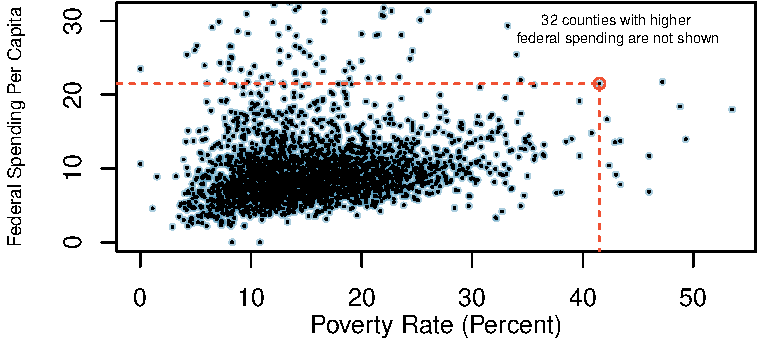
\includegraphics{05-Numerical-Data_files/figure-pdf/fig-scat5-1.pdf}

}

\caption{\label{fig-scat5}A scatterplot showing fed\_spend against
poverty. Owsley County of Kentucky, with a poverty rate of 41.5\% and
federal spending of \$21.50 per capita, is highlighted.}

\end{figure}%

Another scatterplot is shown in Figure~\ref{fig-scat52}, comparing the
number of \texttt{line\_breaks} and number of characters,
\texttt{num\_char}, in emails for the \texttt{email50} data set. In any
scatterplot, each point represents a single case. Since there are 50
cases in \texttt{email50}, there are 50 points in
Figure~\ref{fig-scat52}.

\begin{figure}

\centering{

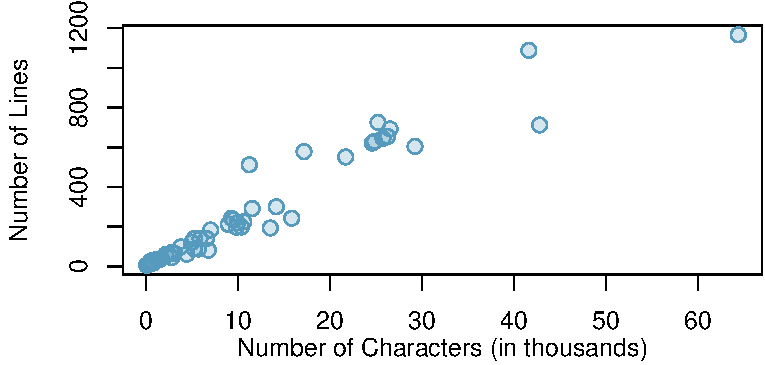
\includegraphics{05-Numerical-Data_files/figure-pdf/fig-scat52-1.pdf}

}

\caption{\label{fig-scat52}A scatterplot of \texttt{line\_breaks} versus
\texttt{num\_char} for the \texttt{email50} data.}

\end{figure}%

To put the number of characters in perspective, this paragraph in the
text has 357 characters. Looking at Figure~\ref{fig-scat52}, it seems
that some emails are incredibly long! Upon further investigation, we
would actually find that most of the long emails use the HTML format,
which means most of the characters in those emails are used to format
the email rather than provide text.

\begin{quote}
\textbf{Exercise}:\\
What do scatterplots reveal about the data, and how might they be
useful?\footnote{Answers may vary. Scatterplots are helpful in quickly
  spotting associations between variables, whether those associations
  represent simple or more complex relationships.}
\end{quote}

\begin{quote}
\emph{Example}:\\
Consider a new data set of 54 cars with two variables: vehicle price and
weight.\footnote{Subset of data from
  http://www.amstat.org/publications/jse/v1n1/datasets.lock.html} A
scatterplot of vehicle price versus weight is shown in
Figure~\ref{fig-scat53}. What can be said about the relationship between
these variables?
\end{quote}

\begin{figure}

\centering{

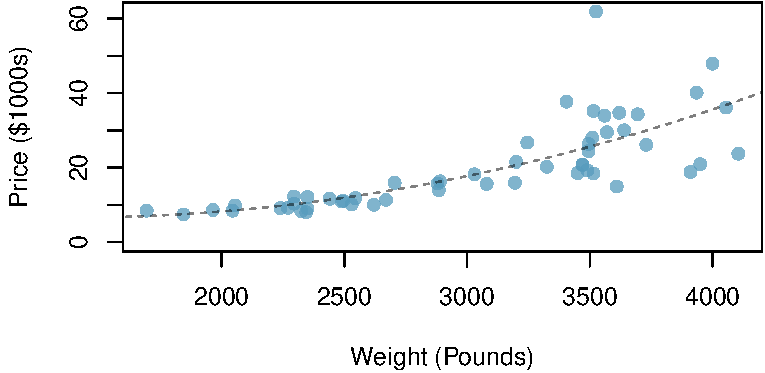
\includegraphics{05-Numerical-Data_files/figure-pdf/fig-scat53-1.pdf}

}

\caption{\label{fig-scat53}A scatterplot of \emph{price} versus
\emph{weight} for 54 cars.}

\end{figure}%

The relationship is evidently nonlinear, as highlighted by the dashed
line. This is different from previous scatterplots we've seen which show
relationships that are very linear.

\begin{quote}
\textbf{Exercise}:\\
Describe two variables that would have a horseshoe-shaped association in
a scatterplot.\footnote{Consider the case where your vertical axis
  represents something ``good'' and your horizontal axis represents
  something that is only good in moderation. Health and water
  consumption fit this description since water becomes toxic when
  consumed in excessive quantities.}
\end{quote}

\subsection{Dot plots and the mean}\label{dot-plots-and-the-mean}

Sometimes two variables are one too many: only one variable may be of
interest. In these cases, a dot plot provides the most basic of
displays. A \textbf{dot plot} is a one-variable scatterplot; an example
using the number of characters from 50 emails is shown in
Figure~\ref{fig-dot5}.

\begin{figure}

\centering{

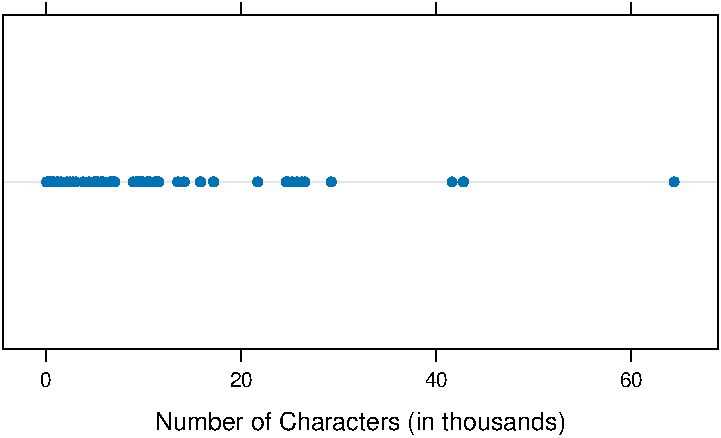
\includegraphics{05-Numerical-Data_files/figure-pdf/fig-dot5-1.pdf}

}

\caption{\label{fig-dot5}A dot plot of \texttt{num\_char} for the
\texttt{email50} data set.}

\end{figure}%

The \textbf{mean}, sometimes called the average, is a common way to
measure the center of a \textbf{distribution}\footnote{The distribution
  of a variable is essentially the collection of all values of the
  variable in the data set. It tells us what values the variable takes
  on and how often. In the \texttt{email50} data set, we used a dotplot
  to view the distribution of \texttt{num\_char}.} of data. To find the
mean number of characters in the 50 emails, we add up all the character
counts and divide by the number of emails. For computational
convenience, the number of characters is listed in the thousands and
rounded to the first decimal.

\[\bar{x} = \frac{21.7 + 7.0 + \cdots + 15.8}{50} = 11.6\]

The sample mean is often labeled \(\bar{x}\). There is a bar over the
letter, and the letter \(x\) is being used as a generic placeholder for
the variable of interest, \texttt{num\_char}.

\begin{quote}
\textbf{Mean}\\
The sample mean of a numerical variable is the sum of all of the
observations divided by the number of observations, Equation 1.
\end{quote}

\begin{equation} 
  \bar{x} = \frac{x_1+x_2+\cdots+x_n}{n}
  \tag{1}
\end{equation}

where \(x_1, x_2, \dots, x_n\) represent the \(n\) observed values.

\begin{quote}
\textbf{Exercise}:\\
Examine the two equations above. What does \(x_1\) correspond to? And
\(x_2\)? Can you infer a general meaning to what \(x_i\) might
represent?\footnote{\(x_1\) corresponds to the number of characters in
  the first email in the sample (21.7, in thousands), \(x_2\) to the
  number of characters in the second email (7.0, in thousands), and
  \(x_i\) corresponds to the number of characters in the \(i^{th}\)
  email in the data set.}
\end{quote}

\begin{quote}
\textbf{Exercise}:\\
What was \(n\) in this sample of emails?\footnote{The sample size,
  \(n = 50\).}
\end{quote}

The \texttt{email50} data set is a sample from a larger population of
emails that were received in January and March. We could compute a mean
for this population in the same way as the sample mean. However, there
is a difference in notation: the population mean has a special label:
\(\mu\). The symbol \(\mu\) is the Greek letter \emph{mu} and represents
the average of all observations in the population. Sometimes a
subscript, such as \(_x\), is used to represent which variable the
population mean refers to, e.g.~\(\mu_x\).

\begin{quote}
\emph{Example}: The average number of characters across all emails can
be estimated using the sample data. Based on the sample of 50 emails,
what would be a reasonable estimate of \(\mu_x\), the mean number of
characters in all emails in the \texttt{email} data set? (Recall that
\texttt{email50} is a sample from \texttt{email}.)
\end{quote}

The sample mean, 11.6, may provide a reasonable estimate of \(\mu_x\).
While this number will not be perfect, it provides a \textbf{point
estimate}, a single plausible value, of the population mean. Later in
the text, we will develop tools to characterize the accuracy of point
estimates, and we will find that point estimates based on larger samples
tend to be more accurate than those based on smaller samples.

\begin{quote}
\emph{Example}:\\
We might like to compute the average income per person in the US. To do
so, we might first think to take the mean of the per capita incomes from
the 3,143 counties in the \texttt{county} data set. What would be a
better approach?
\end{quote}

The \texttt{county} data set is special in that each county actually
represents many individual people. If we were to simply average across
the \texttt{income} variable, we would be treating counties with 5,000
and 5,000,000 residents equally in the calculations. Instead, we should
compute the total income for each county, add up all the counties'
totals, and then divide by the number of people in all the counties. If
we completed these steps with the \texttt{county} data, we would find
that the per capita income for the US is \$27,348.43. Had we computed
the \emph{simple} mean of per capita income across counties, the result
would have been just \$22,504.70!

This previous example used what is called a \textbf{weighted
mean}\footnote{A weighted mean is an average in which some observations
  contribute more ``weight'' than others. In the \texttt{county} data
  set, we ``weighted'' the income for each county by dividing income by
  the county population.}, which will be a key topic in the probability
section. As a look ahead, the probability mass function gives the
population proportions of each county's mean value, and thus, to find
the population mean \(\mu\), we will use a weighted mean.

\subsection{Histograms and shape}\label{histograms-and-shape}

Dot plots show the exact value of each observation. This is useful for
small data sets, but they can become hard to read with larger samples.
Rather than showing the value of each observation, think of the value as
belonging to a \emph{bin}. For example, in the \texttt{email50} data
set, we create a table of counts for the number of cases with character
counts between 0 and 5,000, then the number of cases between 5,000 and
10,000, and so on. Observations that fall on the boundary of a bin
(e.g.~5,000) are allocated to the lower bin. This tabulation is shown
below.

\begin{verbatim}

  (0,5]  (5,10] (10,15] (15,20] (20,25] (25,30] (30,35] (35,40] (40,45] (45,50] 
     19      12       6       2       3       5       0       0       2       0 
(50,55] (55,60] (60,65] 
      0       0       1 
\end{verbatim}

These binned counts are plotted as bars in Figure~\ref{fig-hist5} in
what is called a \textbf{histogram}\footnote{A histogram displays the
  distribution of a quantitative variable. It shows binned counts, the
  number of observations in a bin, or range of values.}.

\begin{figure}

\centering{

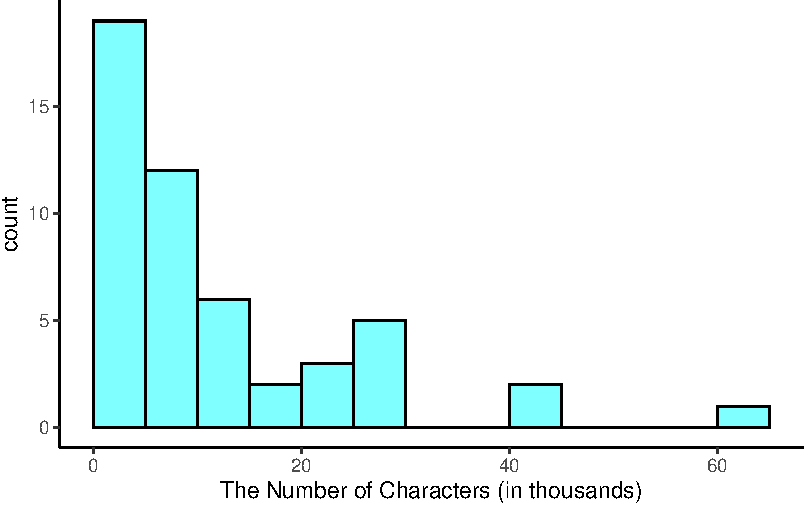
\includegraphics{05-Numerical-Data_files/figure-pdf/fig-hist5-1.pdf}

}

\caption{\label{fig-hist5}A histogram of \texttt{num\_char}. This
distribution is very strongly skewed to the right.}

\end{figure}%

Histograms provide a view of the \textbf{data density}. Higher bars
represent where the data are relatively more dense. For instance, there
are many more emails between 0 and 10,000 characters than emails between
10,000 and 20,000 characters in the data set. The bars make it easy to
see how the density of the data changes relative to the number of
characters.

Histograms are especially convenient for describing the shape of the
data distribution. Figure~\ref{fig-hist5} shows that most emails have a
relatively small number of characters, while fewer emails have a very
large number of characters. When data trail off to the right in this way
and have a longer right \textbf{tail}, the shape is said to be
\textbf{right skewed}.\footnote{Other ways to describe data that are
  skewed to the right: \textbf{skewed to the right}, \textbf{skewed to
  the high end}, or \textbf{skewed to the positive end}.}

Data sets with the reverse characteristic -- a long, thin tail to the
left -- are said to be \textbf{left skewed}. We also say that such a
distribution has a long left tail. Data sets that show roughly equal
trailing off in both directions are called \textbf{symmetric}.

\begin{quote}
\textbf{Long tails to identify skew}\\
When data trail off in one direction, the distribution has a
\textbf{long tail}. If a distribution has a long left tail, it is left
skewed. If a distribution has a long right tail, it is right skewed.
\end{quote}

\begin{quote}
\textbf{Exercise}:\\
Take a look at the dot plot above, Figure~\ref{fig-dot5}. Can you see
the skew in the data? Is it easier to see the skew in this histogram or
the dot plots?\footnote{The skew is visible in both plots, though the
  dot plot is the least useful.}
\end{quote}

\begin{quote}
\textbf{Exercise}:\\
Besides the mean, what can you see in the dot plot that you cannot see
in the histogram?\footnote{Character counts for individual emails.}
\end{quote}

\subsubsection{Making our own histogram}\label{making-our-own-histogram}

Let's take some time to make a simple histogram. We will use the
\textbf{ggformula} package, which is a wrapper for the \textbf{ggplot2}
package.

Here are two questions:\\
\emph{What do we want \texttt{R} to do?} and\\
\emph{What must we give \texttt{R} for it to do this?}

We want \texttt{R} to make a histogram. In \texttt{ggformula}, the plots
have the form \texttt{gf\_plottype} so we will use the
\texttt{gf\_histogram()}. To find options and more information about the
function, type:

\begin{verbatim}
?gf_histogram
\end{verbatim}

To start, we just have to give the formulas and data to \texttt{R}.

\begin{Shaded}
\begin{Highlighting}[]
\FunctionTok{gf\_histogram}\NormalTok{(}\SpecialCharTok{\textasciitilde{}}\NormalTok{num\_char, }\AttributeTok{data =}\NormalTok{ email50, }\AttributeTok{color =} \StringTok{"black"}\NormalTok{, }\AttributeTok{fill =} \StringTok{"cyan"}\NormalTok{)}
\end{Highlighting}
\end{Shaded}

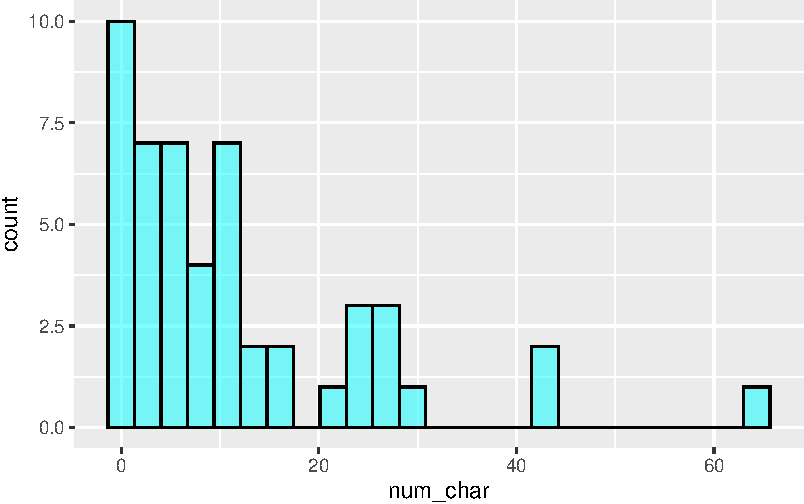
\includegraphics{05-Numerical-Data_files/figure-pdf/unnamed-chunk-9-1.pdf}

\begin{quote}
\textbf{Exercise}:\\
Look at the help menu for \texttt{gf\_histogram} and change the x-axis
label, change the bin width to 5, and have the left bin start at 0.
\end{quote}

Here is the code for the exercise:

\begin{verbatim}
email50 %>%
   gf_histogram(~num_char, binwidth = 5,boundary = 0,
   xlab = "The Number of Characters (in thousands)", 
   color = "black", fill = "cyan") %>%
   gf_theme(theme_classic())
\end{verbatim}

In addition to looking at whether a distribution is skewed or symmetric,
histograms can be used to identify modes. A \textbf{mode} is represented
by a prominent peak in the distribution.\footnote{Another definition of
  mode, which is not typically used in statistics, is the value with the
  most occurrences. It is common to have \emph{no} observations with the
  same value in a data set, which makes this other definition useless
  for many real data sets.} There is only one prominent peak in the
histogram of \texttt{num\_char}.

Figure~\ref{fig-histmulti} shows histograms that have one, two, or three
prominent peaks. Such distributions are called \textbf{unimodal},
\textbf{bimodal}, and \textbf{multimodal}, respectively. Any
distribution with more than 2 prominent peaks is called multimodal.
Notice that there was one prominent peak in the unimodal distribution
with a second less prominent peak that was not counted since the
separation between the two peaks is relatively small, and it only
differs from its neighboring bins by a few observations.

\begin{figure}

\centering{

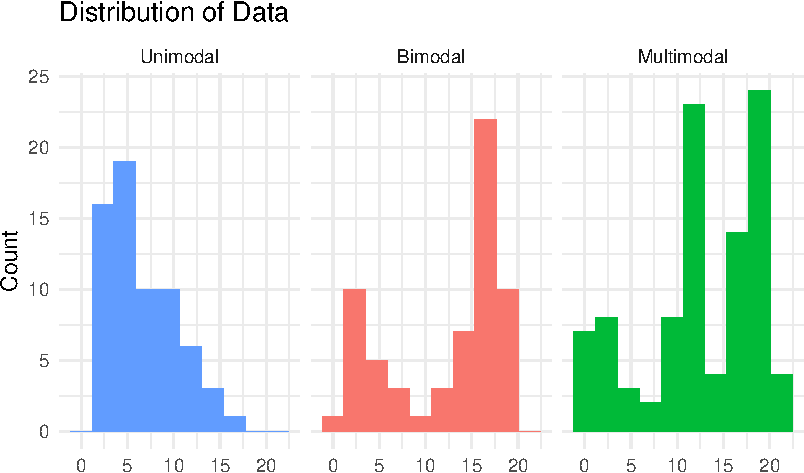
\includegraphics{05-Numerical-Data_files/figure-pdf/fig-histmulti-1.pdf}

}

\caption{\label{fig-histmulti}Histograms that demonstrate unimodal,
bimodal, and multimodal data.}

\end{figure}%

\begin{quote}
\textbf{Exercise}:\\
Height measurements of young students and adult teachers at a K-3
elementary school were taken. How many modes would you anticipate in
this height data set?\footnote{There might be two height groups visible
  in the data set: one for the students and one for the adults. That is,
  the data are probably bimodal. But it could be multimodal because
  within each group we may be able to see a difference in males and
  females.}
\end{quote}

\begin{quote}
\textbf{Looking for modes}\\
Looking for modes isn't about finding a clear and correct answer about
the number of modes in a distribution, which is why \textbf{prominent}
is not rigorously defined in these notes. The important part of this
examination is to better understand your data and how it might be
structured.
\end{quote}

\subsection{Variance and standard
deviation}\label{variance-and-standard-deviation}

The mean is used to describe the center of a data set, but the
\emph{variability} in the data is also important. Here, we introduce two
measures of variability: the \textbf{variance} and the \textbf{standard
deviation}. Both of these are very useful in data analysis, even though
the formulas are a bit tedious to calculate by hand. The standard
deviation is the easier of the two to conceptually understand; it
roughly describes how far away the typical observation is from the mean.
Equation 2 is the equation for sample variance. We will demonstrate it
with data so that the notation is easier to understand.

\begin{align}
s_{}^2 &= \sum_{i = 1}^{n} \frac{(x_i - \bar{x})^2}{n - 1} \\
    &= \frac{(x_1 - \bar{x})^2 + (x_2 - \bar{x})^2 + (x_3 - \bar{x})^2 + \cdots + (x_n - \bar{x})^2}{n - 1} 
  \tag{2}
\end{align}

where \(x_1, x_2, \dots, x_n\) represent the \(n\) observed values.

We call the distance of an observation from its mean the
\textbf{deviation}. Below are the deviations for the \(1^{st}\),
\(2^{nd}\), \(3^{rd}\), and \(50^{th}\) observations of the
\texttt{num\_char} variable. For computational convenience, the number
of characters is listed in the thousands and rounded to the first
decimal.

\[
\begin{aligned}
x_1^{}-\bar{x} &= 21.7 - 11.6 = 10.1 \hspace{5mm}\text{ } \\
x_2^{}-\bar{x} &= 7.0 - 11.6 = -4.6 \\
x_3^{}-\bar{x} &= 0.6 - 11.6 = -11.0 \\
            &\ \vdots \\
x_{50}^{}-\bar{x} &= 15.8 - 11.6 = 4.2
\end{aligned}
\]

If we square these deviations and then take an average, the result is
equal to the \textbf{sample variance}, denoted by \(s_{}^2\):

\[
\begin{aligned}
s_{}^2 &= \frac{10.1_{}^2 + (-4.6)_{}^2 + (-11.0)_{}^2 + \cdots + 4.2_{}^2}{50-1} \\
    &= \frac{102.01 + 21.16 + 121.00 + \cdots + 17.64}{49} \\
    &= 172.44
\end{aligned}
\]

We divide by \(n - 1\), rather than dividing by \(n\), when computing
the variance; you need not worry about this mathematical nuance yet.
Notice that squaring the deviations does two things. First, it makes
large values much larger, seen by comparing \(10.1^2\), \((-4.6)^2\),
\((-11.0)^2\), and \(4.2^2\). Second, it gets rid of any negative signs.

The sample \textbf{standard deviation}, \(s\), is the square root of the
variance:

\[s = \sqrt{172.44} = 13.13\]

The sample standard deviation of the number of characters in an email is
13.13 thousand. A subscript of \(_x\) may be added to the variance and
standard deviation, i.e.~\(s_x^2\) and \(s_x^{}\), as a reminder that
these are the variance and standard deviation of the observations
represented by \(x_1^{}\), \(x_2^{}\), \ldots, \(x_n^{}\). The \(_{x}\)
subscript is usually omitted when it is clear which data the variance or
standard deviation is referencing.

\begin{quote}
\textbf{Variance and standard deviation}\\
The variance is roughly the average squared distance from the mean. The
standard deviation is the square root of the variance and describes how
close the data are to the mean.
\end{quote}

Formulas and methods used to compute the variance and standard deviation
for a population are similar to those used for a sample.\footnote{The
  only difference is that the population variance has a division by
  \(n\) instead of \(n - 1\).} However, like the mean, the population
values have special symbols: \(\sigma_{}^2\) for the variance and
\(\sigma\) for the standard deviation. The symbol \(\sigma\) is the
Greek letter \emph{sigma}.

\begin{quote}
\textbf{Tip: standard deviation describes variability}\\
Focus on the conceptual meaning of the standard deviation as a
descriptor of variability rather than the formulas. Usually 70\% of the
data will be within one standard deviation of the mean and about 95\%
will be within two standard deviations. However, as we have seen, these
percentages are not strict rules.
\end{quote}

\begin{figure}

\centering{

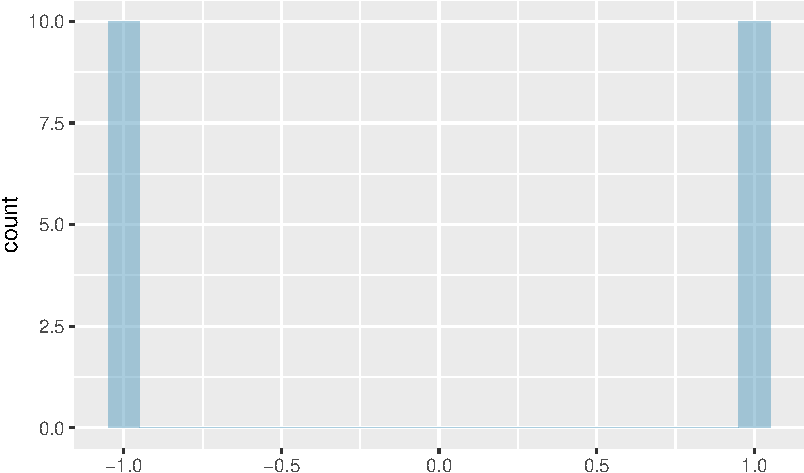
\includegraphics{05-Numerical-Data_files/figure-pdf/fig-hist53-1.pdf}

}

\caption{\label{fig-hist53}The first of three very different population
distributions with the same mean, 0, and standard deviation, 1.}

\end{figure}%

\begin{figure}

\centering{

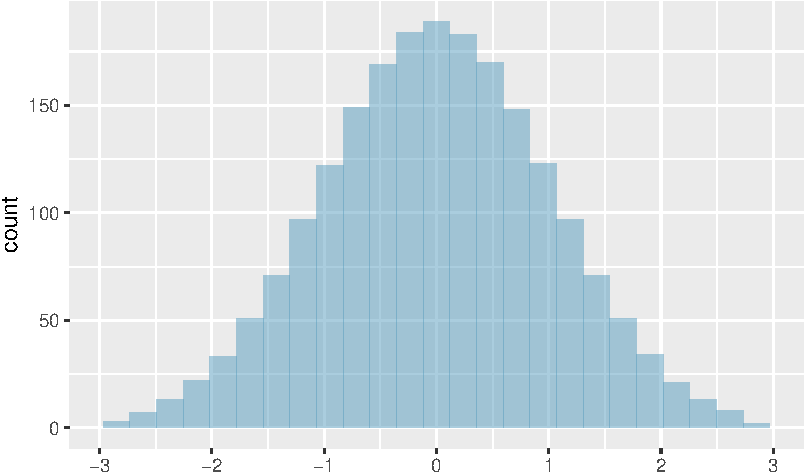
\includegraphics{05-Numerical-Data_files/figure-pdf/fig-hist54-1.pdf}

}

\caption{\label{fig-hist54}The second plot with mean 0 and standard
deviation 1.}

\end{figure}%

\begin{figure}

\centering{

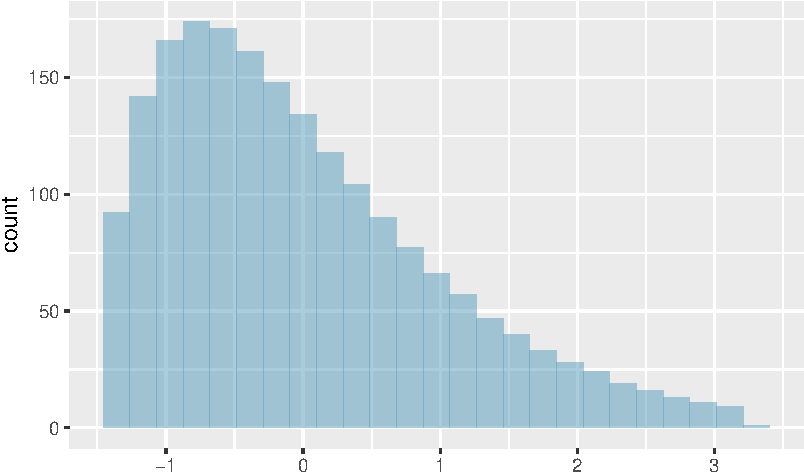
\includegraphics{05-Numerical-Data_files/figure-pdf/fig-hist55-1.pdf}

}

\caption{\label{fig-hist55}The final plot with mean 0 and standard
deviation 1.}

\end{figure}%

\begin{quote}
\textbf{Exercise}:\\
Earlier, the concept of shape of a distribution was introduced. A good
description of the shape of a distribution should include modality and
whether the distribution is symmetric or skewed to one side. Using the
three figures,
Figures~\ref{fig-hist53}, \ref{fig-hist54}, \ref{fig-hist55} as
examples, explain why such a description is important.\footnote{Starting
  with Figure @ref(fig:hist53-fig), the three figures show three
  distributions that look quite different, but all have the same mean,
  variance, and standard deviation. Using modality, we can distinguish
  between the first plot (bimodal) and the last two (unimodal). Using
  skewness, we can distinguish between the last plot (right skewed) and
  the first two. While a picture, like a histogram, tells a more
  complete story, we can use modality and shape (symmetry/skew) to
  characterize basic information about a distribution.}
\end{quote}

\begin{quote}
\emph{Example}:\\
Describe the distribution of the \texttt{num\_char} variable using the
histogram in Figure~\ref{fig-hist5}. The description should incorporate
the center, variability, and shape of the distribution, and it should
also be placed in context: the number of characters in emails. Also note
any especially unusual cases/observations.\footnote{The distribution of
  email character counts is unimodal and very strongly skewed to the
  high end (right skewed). Many of the counts fall near the mean at
  11,600, and most fall within one standard deviation (13,130) of the
  mean. There is one exceptionally long email with about 65,000
  characters.}
\end{quote}

In practice, the variance and standard deviation are sometimes used as a
means to an end, where the \emph{end} is being able to accurately
estimate the uncertainty associated with a sample statistic. For
example, later in the book we will use the variance and standard
deviation to assess how close the sample mean is to the population mean.

\subsection{Box plots, quartiles, and the
median}\label{box-plots-quartiles-and-the-median}

A \textbf{box plot} summarizes a data set using five statistics, while
also plotting unusual observations. Figure~\ref{fig-box} provides an
annotated vertical dot plot alongside a box plot of the
\texttt{num\_char} variable from the \texttt{email50} data set.

\begin{figure}

\centering{

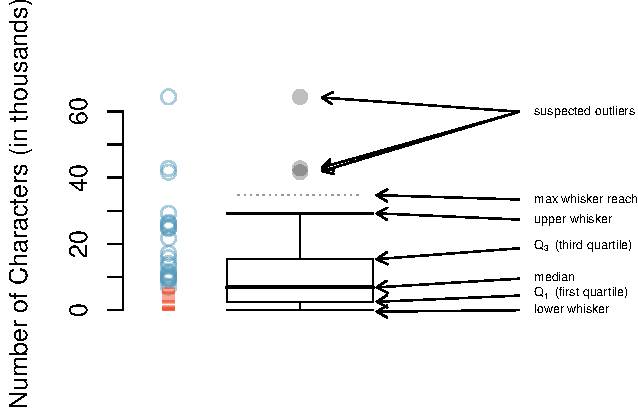
\includegraphics{05-Numerical-Data_files/figure-pdf/fig-box-1.pdf}

}

\caption{\label{fig-box}A vertical dot plot next to a labeled box plot
for the number of characters in 50 emails. The median (6,890), splits
the data into the bottom 50\% and the top 50\%, marked in the dot plot
by horizontal dashes and open circles, respectively.}

\end{figure}%

The first step in building a box plot is drawing a dark line denoting
the \textbf{median}, which splits the data in half. Figure~\ref{fig-box}
shows 50\% of the data falling below the median (red dashes) and the
other 50\% falling above the median (blue open circles). There are 50
character counts in the data set (an even number) so the data are
perfectly split into two groups of 25. We take the median in this case
to be the average of the two observations closest to the \(50^{th}\)
percentile: \((\text{6,768} + \text{7,012}) / 2 = \text{6,890}\). When
there are an odd number of observations, there will be exactly one
observation that splits the data into two halves, and in this case that
observation is the median (no average needed).

\begin{quote}
\textbf{Median: the number in the middle}\\
If the data are ordered from smallest to largest, the \textbf{median} is
the observation in the middle. If there are an even number of
observations, there will be two values in the middle, and the median is
taken as their average.
\end{quote}

The second step in building a box plot is drawing a rectangle to
represent the middle 50\% of the data. The total length of the box,
shown vertically in Figure~\ref{fig-box}, is called the
\textbf{interquartile range} (IQR, for short). It, like the standard
deviation, is a measure of variability in the data. The more variable
the data, the larger the standard deviation and IQR. The two boundaries
of the box are called the \textbf{first quartile} (the \(25^{th}\)
percentile, i.e.~25\% of the data fall below this value) and the
\textbf{third quartile} (the \(75^{th}\) percentile), and these are
often labeled \(Q_1\) and \(Q_3\), respectively.

\begin{quote}
\textbf{Interquartile range (IQR)}\\
The IQR is the length of the box in a box plot. It is computed as
\[ IQR = Q_3 - Q_1 \] where \(Q_1\) and \(Q_3\) are the \(25^{th}\) and
\(75^{th}\) percentiles, respectively.
\end{quote}

\begin{quote}
\textbf{Exercise}:\\
What percent of the data fall between \(Q_1\) and the median? What
percent is between the median and \(Q_3\)?\footnote{Since \(Q_1\) and
  \(Q_3\) capture the middle 50\% of the data and the median splits the
  data in the middle, 25\% of the data fall between \(Q_1\) and the
  median, and another 25\% fall between the median and \(Q_3\).}
\end{quote}

Extending out from the box, the \textbf{whiskers} attempt to capture the
data outside of the box, however, their reach is never allowed to be
more than \(1.5\times IQR\).\footnote{While the choice of exactly 1.5 is
  arbitrary, it is the most commonly used value for box plots.} They
capture everything within this reach. In Figure~\ref{fig-box}, the upper
whisker does not extend to the last three points, which are beyond
\(Q_3 + 1.5\times IQR\), and so it extends only to the last point below
this limit. The lower whisker stops at the lowest value, 33, since there
is no additional data to reach; the lower whisker's limit is not shown
in the figure because the plot does not extend down to
\(Q_1 - 1.5\times IQR\). In a sense, the box is like the body of the box
plot and the whiskers are like its arms trying to reach the rest of the
data.

Any observation that lies beyond the whiskers is labeled with a dot. The
purpose of labeling these points -- instead of just extending the
whiskers to the minimum and maximum observed values -- is to help
identify any observations that appear to be unusually distant from the
rest of the data. Unusually distant observations are called
\textbf{outliers}. In this case, it would be reasonable to classify the
emails with character counts of 41,623, 42,793, and 64,401 as outliers
since they are numerically distant from most of the data.

\begin{quote}
\textbf{Outliers are extreme}\\
An \textbf{outlier} is an observation that is extreme, relative to the
rest of the data.
\end{quote}

\begin{quote}
\textbf{Why it is important to look for outliers}\\
Examination of data for possible outliers serves many useful purposes,
including:\\
1. Identifying \textbf{strong skew} in the distribution.\\
2. Identifying data collection or entry errors. For instance, we
re-examined the email purported to have 64,401 characters to ensure this
value was accurate.\\
3. Providing insight into interesting properties of the data.
\end{quote}

\begin{quote}
\textbf{Exercise}:\\
The observation with value 64,401, an outlier, was found to be an
accurate observation. What would such an observation suggest about the
nature of character counts in emails?\footnote{That occasionally there
  may be very long emails.}
\end{quote}

\begin{quote}
\textbf{Exercise}:\\
Using Figure~\ref{fig-box}, estimate the following values for
\texttt{num\_char} in the \texttt{email50} data set:\\
(a) \(Q_1\),\\
(b) \(Q_3\), and\\
(c) IQR.\footnote{These visual estimates will vary a little from one
  person to the next: \(Q_1\) \textasciitilde{} 3,000, \(Q_3\)
  \textasciitilde{} 15,000, IQR = \(Q_3 - Q_1\) \textasciitilde{}
  12,000. (The true values: \$Q\_1 = \$ 2,536, \$Q\_3 = \$ 15,411, IQR =
  12,875.)}
\end{quote}

Of course, \texttt{R} can calculate these summary statistics for us.
First, we will do these calculations individually and then in one
function call. Remember to ask yourself what you want \texttt{R} to do
and what it needs to do this.

\begin{Shaded}
\begin{Highlighting}[]
\FunctionTok{mean}\NormalTok{(}\SpecialCharTok{\textasciitilde{}}\NormalTok{num\_char, }\AttributeTok{data =}\NormalTok{ email50)}
\end{Highlighting}
\end{Shaded}

\begin{verbatim}
[1] 11.59822
\end{verbatim}

\begin{Shaded}
\begin{Highlighting}[]
\FunctionTok{sd}\NormalTok{(}\SpecialCharTok{\textasciitilde{}}\NormalTok{num\_char, }\AttributeTok{data =}\NormalTok{ email50)}
\end{Highlighting}
\end{Shaded}

\begin{verbatim}
[1] 13.12526
\end{verbatim}

\begin{Shaded}
\begin{Highlighting}[]
\FunctionTok{quantile}\NormalTok{(}\SpecialCharTok{\textasciitilde{}}\NormalTok{num\_char, }\AttributeTok{data =}\NormalTok{ email50)}
\end{Highlighting}
\end{Shaded}

\begin{verbatim}
      0%      25%      50%      75%     100% 
 0.05700  2.53550  6.88950 15.41075 64.40100 
\end{verbatim}

\begin{Shaded}
\begin{Highlighting}[]
\FunctionTok{iqr}\NormalTok{(}\SpecialCharTok{\textasciitilde{}}\NormalTok{num\_char, }\AttributeTok{data =}\NormalTok{ email50)}
\end{Highlighting}
\end{Shaded}

\begin{verbatim}
[1] 12.87525
\end{verbatim}

\begin{Shaded}
\begin{Highlighting}[]
\FunctionTok{favstats}\NormalTok{(}\SpecialCharTok{\textasciitilde{}}\NormalTok{num\_char, }\AttributeTok{data =}\NormalTok{ email50)}
\end{Highlighting}
\end{Shaded}

\begin{verbatim}
   min     Q1 median       Q3    max     mean       sd  n missing
 0.057 2.5355 6.8895 15.41075 64.401 11.59822 13.12526 50       0
\end{verbatim}

\subsection{Robust statistics}\label{robust-statistics}

How are the \emph{sample statistics} of the \texttt{num\_char} data set
affected by the observation with value 64,401? What would we see if this
email wasn't present in the data set? What would happen to these
\emph{summary statistics} if the observation at 64,401 had been even
larger, say 150,000? These scenarios are plotted alongside the original
data in Figure~\ref{fig-box2}, and sample statistics are computed in
\texttt{R}.

First, we create a new data frame containing the three scenarios: 1) the
original data, 2) the data with the extreme observation dropped, and 3)
the data with the extreme observation increased.

\begin{Shaded}
\begin{Highlighting}[]
\CommentTok{\# code to create the \textasciigrave{}robust\textasciigrave{} data frame}
\NormalTok{p1 }\OtherTok{\textless{}{-}}\NormalTok{ email50}\SpecialCharTok{$}\NormalTok{num\_char}
\NormalTok{p2 }\OtherTok{\textless{}{-}}\NormalTok{ p1[}\SpecialCharTok{{-}}\FunctionTok{which.max}\NormalTok{(p1)]}
\NormalTok{p3 }\OtherTok{\textless{}{-}}\NormalTok{ p1}
\NormalTok{p3[}\FunctionTok{which.max}\NormalTok{(p1)] }\OtherTok{\textless{}{-}} \DecValTok{150}

\NormalTok{robust }\OtherTok{\textless{}{-}} \FunctionTok{data.frame}\NormalTok{(}\AttributeTok{value =} \FunctionTok{c}\NormalTok{(p1, p2, p3),}
                     \AttributeTok{group =} \FunctionTok{c}\NormalTok{(}\FunctionTok{rep}\NormalTok{(}\StringTok{"Original"}\NormalTok{, }\DecValTok{50}\NormalTok{),}
                             \FunctionTok{rep}\NormalTok{(}\StringTok{"Dropped"}\NormalTok{, }\DecValTok{49}\NormalTok{), }\FunctionTok{rep}\NormalTok{(}\StringTok{"Increased"}\NormalTok{, }\DecValTok{50}\NormalTok{)))}
\FunctionTok{head}\NormalTok{(robust)}
\end{Highlighting}
\end{Shaded}

\begin{verbatim}
   value    group
1 21.705 Original
2  7.011 Original
3  0.631 Original
4  2.454 Original
5 41.623 Original
6  0.057 Original
\end{verbatim}

Now, we create a side-by-side boxplots for each scenario.

\begin{Shaded}
\begin{Highlighting}[]
\FunctionTok{gf\_boxplot}\NormalTok{(value }\SpecialCharTok{\textasciitilde{}}\NormalTok{ group, }\AttributeTok{data =}\NormalTok{ robust, }\AttributeTok{xlab =} \StringTok{"Data Group"}\NormalTok{,}
           \AttributeTok{ylab =} \StringTok{"Number of Characters (in thousands)"}\NormalTok{) }\SpecialCharTok{\%\textgreater{}\%}
   \FunctionTok{gf\_theme}\NormalTok{(}\FunctionTok{theme\_classic}\NormalTok{())}
\end{Highlighting}
\end{Shaded}

\begin{figure}[H]

\centering{

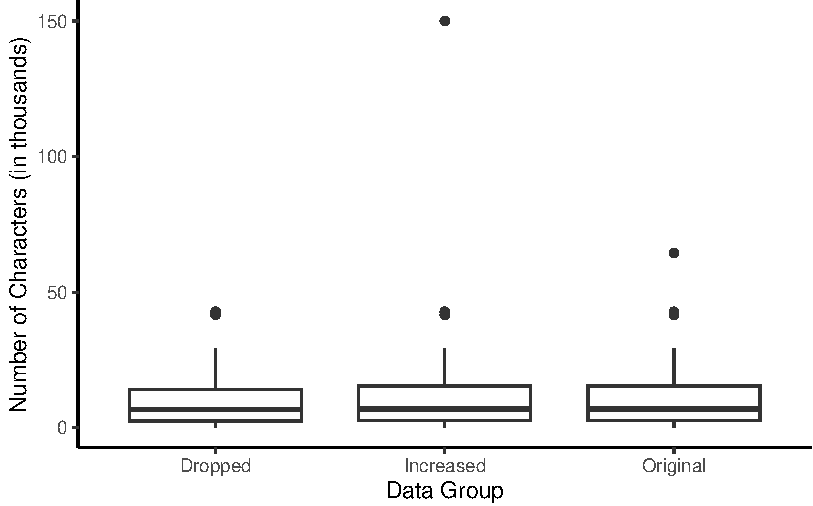
\includegraphics{05-Numerical-Data_files/figure-pdf/fig-box2-1.pdf}

}

\caption{\label{fig-box2}Box plots of the original character count data
and two modified data sets, one where the outlier at 64,401 is dropped
and one where its value is increased.}

\end{figure}%

We can also use \texttt{favstats()} to calculate summary statistics of
\texttt{value} by \texttt{group}, using the \texttt{robust} data frame
created above.

\begin{Shaded}
\begin{Highlighting}[]
\FunctionTok{favstats}\NormalTok{(value }\SpecialCharTok{\textasciitilde{}}\NormalTok{ group, }\AttributeTok{data =}\NormalTok{ robust)}
\end{Highlighting}
\end{Shaded}

\begin{verbatim}
      group   min     Q1 median       Q3     max     mean       sd  n missing
1   Dropped 0.057 2.4540 6.7680 14.15600  42.793 10.52061 10.79768 49       0
2 Increased 0.057 2.5355 6.8895 15.41075 150.000 13.31020 22.43436 50       0
3  Original 0.057 2.5355 6.8895 15.41075  64.401 11.59822 13.12526 50       0
\end{verbatim}

Notice by using the formula notation, we were able to calculate the
summary statistics within each group.

\begin{quote}
\textbf{Exercise}:\\
(a) Which is affected more by extreme observations, the mean or median?
The data summary may be helpful.\footnote{The mean is affected more.}\\
(b) Which is affected more by extreme observations, the standard
deviation or IQR?\footnote{The standard deviation is affected more.}
\end{quote}

The median and IQR are called \textbf{robust statistics} because extreme
observations have little effect on their values. The mean and standard
deviation are affected much more by changes in extreme observations.

\begin{quote}
\emph{Example}:\\
The median and IQR do not change much under the three scenarios above.
Why might this be the case?\footnote{The median and IQR are only
  sensitive to numbers near \(Q_1\), the median, and \(Q_3\). Since
  values in these regions are relatively stable -- there aren't large
  jumps between observations -- the median and IQR estimates are also
  quite stable.}
\end{quote}

\begin{quote}
\textbf{Exercise}:\\
The distribution of vehicle prices tends to be right skewed, with a few
luxury and sports cars lingering out into the right tail. If you were
searching for a new car and cared about price, should you be more
interested in the mean or median price of vehicles sold, assuming you
are in the market for a regular car?\footnote{Buyers of a \emph{regular
  car} should be more concerned about the median price. High-end car
  sales can drastically inflate the mean price while the median will be
  more robust to the influence of those sales.}
\end{quote}

\subsection{Transforming data}\label{transforming-data}

When data are very strongly skewed, we sometimes transform them so they
are easier to model. Consider the histogram of Major League Baseball
players' salaries from 2010, which is shown in Figure~\ref{fig-hist510}.

\begin{figure}

\centering{

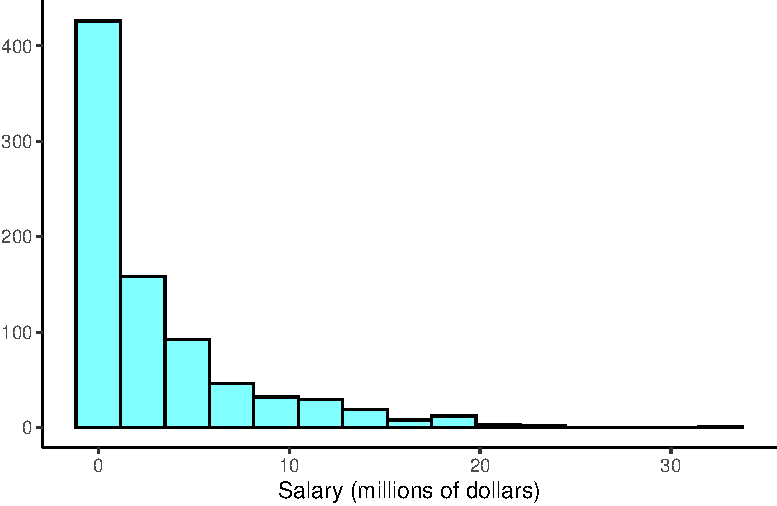
\includegraphics{05-Numerical-Data_files/figure-pdf/fig-hist510-1.pdf}

}

\caption{\label{fig-hist510}Histogram of MLB player salaries for 2010,
in millions of dollars.}

\end{figure}%

\begin{quote}
\emph{Example}:\\
The histogram of MLB player salaries is somewhat useful because we can
see that the data are extremely skewed and centered (as gauged by the
median) at about \$1 million. What about this plot is not
useful?\footnote{Most of the data are collected into one bin in the
  histogram and the data are so strongly skewed that many details in the
  data are obscured.}
\end{quote}

There are some standard transformations that are often applied when much
of the data cluster near zero (relative to the larger values in the data
set) and all observations are positive. A \textbf{transformation} is a
rescaling of the data using a function. For instance, a plot of the
natural logarithm\footnote{Statisticians often write the natural
  logarithm as \(\log\). You might be more familiar with it being
  written as \(\ln\).} of player salaries results in a new histogram in
Figure~\ref{fig-hist512}. Transformed data are sometimes easier to work
with when applying statistical models because the transformed data are
much less skewed and outliers are usually less extreme.

\begin{figure}

\centering{

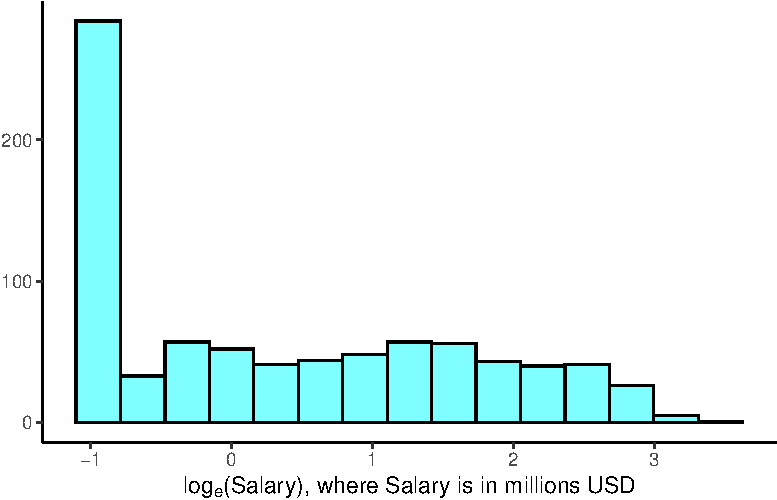
\includegraphics{05-Numerical-Data_files/figure-pdf/fig-hist512-1.pdf}

}

\caption{\label{fig-hist512}Histogram of the log-transformed MLB player
salaries for 2010.}

\end{figure}%

Transformations can also be applied to one or both variables in a
scatterplot. A scatterplot of the original \texttt{line\_breaks} and
\texttt{num\_char} variables is shown in Figure~\ref{fig-scat52} above.
We can see a positive association between the variables and that many
observations are clustered near zero. Later in this text, we might want
to use a straight line to model the data. However, we'll find that the
data in their current state cannot be modeled very well.
Figure~\ref{fig-scat513} shows a scatterplot where both
\texttt{line\_breaks} and \texttt{num\_char} have been transformed using
a natural log (log base \(e\)) transformation. While there is a positive
association in each plot, the transformed data show a steadier trend,
which is easier to model than the original (un-transformed) data.

\begin{figure}

\centering{

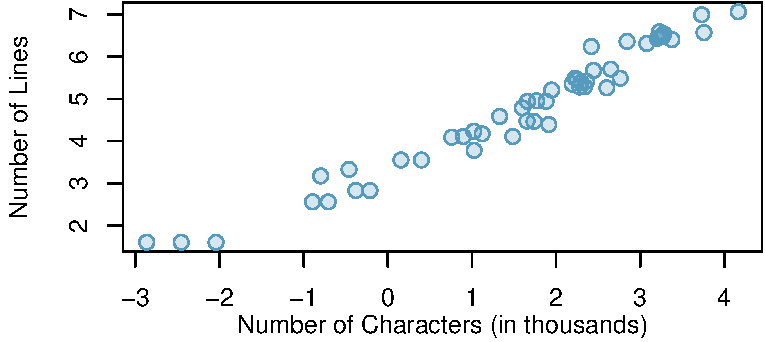
\includegraphics{05-Numerical-Data_files/figure-pdf/fig-scat513-1.pdf}

}

\caption{\label{fig-scat513}A scatterplot of \texttt{line\_breaks}
versus \texttt{num\_char} for the \texttt{email50} data, where both
variables have been log-transformed.}

\end{figure}%

Transformations other than the logarithm can be useful, too. For
instance, the square root (\(\sqrt{\text{original observation}}\)) and
inverse \(\left(\frac{1}{\text{original observation}}\right)\) are used
commonly by statisticians. Common goals in transforming data are to see
the data structure differently, reduce skew, assist in modeling, or
straighten a nonlinear relationship in a scatterplot.

\section{Homework Problems}\label{homework-problems-4}

Create an Rmd file for the work including headers, file creation data,
and explanation of your work. Make sure your plots have a title and the
axes are labeled.

\begin{enumerate}
\def\labelenumi{\arabic{enumi}.}
\tightlist
\item
  \textbf{Mammals exploratory}. Data were collected on 39 species of
  mammals distributed over 13 taxonomic orders. The data is in the
  \texttt{mammals} data set in the \textbf{openintro} package.
\end{enumerate}

\begin{enumerate}
\def\labelenumi{\alph{enumi}.}
\item
  Using the documentation for the \texttt{mammals} data set, report the
  units for the variable \texttt{brain\_wt}.
\item
  Using \texttt{inspect()}, how many variables are numeric?
\item
  What type of variable is \texttt{danger}?
\item
  Create a histogram of \texttt{total\_sleep} and describe the
  distribution.
\item
  Create a boxplot of \texttt{life\_span} and describe the distribution.
\item
  Report the mean and median life span of a mammal.
\item
  Calculate the summary statistics for \texttt{life\_span} broken down
  by \texttt{danger}. What is the standard deviation of life span in
  danger outcome 5?
\end{enumerate}

\begin{enumerate}
\def\labelenumi{\arabic{enumi}.}
\setcounter{enumi}{1}
\tightlist
\item
  \textbf{Mammal life spans}. Continue using the \texttt{mammals} data
  set.
\end{enumerate}

\begin{enumerate}
\def\labelenumi{\alph{enumi}.}
\item
  Create side-by-side boxplots for \texttt{life\_span} broken down by
  \texttt{exposure}. Note: you will have to change \texttt{exposure} to
  a \texttt{factor()}. Report on any findings.
\item
  What happened to the median and third quartile in exposure group 4?
\item
  Using the same variables, create faceted histograms. What are the
  shortcomings of this plot?
\item
  Create a new variable \texttt{exposed} that is a factor with level
  \texttt{Low} if exposure is \texttt{1} or \texttt{2} and \texttt{High}
  otherwise.
\item
  Repeat part c) with the new \texttt{exposed} variable. Explain what
  you see in the plot.
\end{enumerate}

\begin{enumerate}
\def\labelenumi{\arabic{enumi}.}
\setcounter{enumi}{2}
\tightlist
\item
  \textbf{Mammal life spans continued}
\end{enumerate}

\begin{enumerate}
\def\labelenumi{\alph{enumi}.}
\item
  Create a scatterplot of life span versus length of gestation.
\item
  What type of association is apparent between life span and length of
  gestation?
\item
  What type of association would you expect to see if the axes of the
  plot were reversed, i.e.~if we plotted length of gestation versus life
  span?
\item
  Create the new scatterplot suggested in part c).
\item
  Are life span and length of gestation independent? Explain your
  reasoning.
\end{enumerate}

\section*{\texorpdfstring{\href{https://ds-usafa.github.io/CPS-Solutions-Manual/NUMDATA.html}{Solutions
Manual}}{Solutions Manual}}\label{solutions-manual-5}
\addcontentsline{toc}{section}{\href{https://ds-usafa.github.io/CPS-Solutions-Manual/NUMDATA.html}{Solutions
Manual}}

\markright{Solutions Manual}

\chapter{Categorical Data}\label{CATDATA}

\section{Objectives}\label{objectives-6}

\begin{enumerate}
\def\labelenumi{\arabic{enumi})}
\item
  Define and use properly in context all new terminology, to include:
  \emph{factor}, \emph{contingency table}, \emph{marginal counts},
  \emph{joint counts}, \emph{frequency table}, \emph{relative frequency
  table}, \emph{bar plot}, \emph{conditioning}, \emph{segmented bar
  plot}, \emph{mosaic plot}, \emph{pie chart}, \emph{side-by-side box
  plot}, \emph{density plot}.
\item
  In \texttt{R}, generate tables for categorical variable(s).
\item
  In \texttt{R}, generate appropriate graphical summaries of categorical
  and numerical variables.
\item
  Interpret and explain output both graphically and numerically.
\end{enumerate}

\section{Categorical data}\label{categorical-data-1}

Like numerical data, categorical data can also be organized and
analyzed. This section introduces tables and other basic tools for use
with categorical data. Remember at the beginning of this block of
material, our case study had categorical data so we have already seen
some of the ideas in this chapter.

The \texttt{email50} data set represents a sample from a larger email
data set called \texttt{email}. This larger data set contains
information on 3,921 emails. In this section, we will use the
\texttt{email} data set to examine whether the presence of numbers,
small or large, in an email provides any useful information in
classifying email as spam or not spam.

\subsection{Contingency tables and bar
plots}\label{contingency-tables-and-bar-plots}

In the \texttt{email} data set, we have two variables, \texttt{spam} and
\texttt{number}, that we want to summarize. Let's use \texttt{inspect()}
to get information and insight about the two variables. We can also type
\texttt{?email} or \texttt{help(email)} to learn more about the data.
First, load the \texttt{openintro} library.

\begin{Shaded}
\begin{Highlighting}[]
\FunctionTok{library}\NormalTok{(openintro)}
\end{Highlighting}
\end{Shaded}

\begin{Shaded}
\begin{Highlighting}[]
\NormalTok{email }\SpecialCharTok{\%\textgreater{}\%}
  \FunctionTok{select}\NormalTok{(spam, number) }\SpecialCharTok{\%\textgreater{}\%}
  \FunctionTok{inspect}\NormalTok{()}
\end{Highlighting}
\end{Shaded}

\begin{verbatim}

categorical variables:  
    name  class levels    n missing
1 number factor      3 3921       0
                                   distribution
1 small (72.1%), none (14%) ...                

quantitative variables:  
  name   class min Q1 median Q3 max       mean        sd    n missing
1 spam numeric   0  0      0  0   1 0.09359857 0.2913066 3921       0
\end{verbatim}

Notice the use of the \texttt{pipe} operator and how it adds to the ease
of reading the code. The \texttt{select()} function allows us to narrow
down the columns/variables to the two of interest. Then
\texttt{inspect()} gives us information about those variables. We read
from top line; we start with the data set \texttt{email}, input it into
\texttt{select()} and select variables from it, and then use
\texttt{inspect()} to summarize the variables.

As indicated above, \texttt{number} is a categorical variable (a
\emph{factor}) that describes whether an email contains no numbers, only
small numbers (values under 1 million), or at least one big number (a
value of 1 million or more). The variable \texttt{spam} is a numeric
variable, where \texttt{1} indicates the email is spam and \texttt{0}
indicates the email is not spam. To treat \texttt{spam} as categorical,
we will want to change it to a \emph{factor}, but first we will build a
table that summarizes data for the two variables
(Table~\ref{tbl-contin1}). This table is called a \textbf{contingency
table}\footnote{A contingency table is a two-way table that shows the
  distribution of one variable in rows and a second variable in columns.}.
Each value in the table represents the number of times a particular
combination of variable outcomes occurred.

\begin{longtable}[t]{lrrrr}

\caption{\label{tbl-contin1}A contingency table for the \texttt{email}
data.}

\tabularnewline

\\
\toprule
\multicolumn{1}{c}{Spam} & \multicolumn{3}{c}{Number} & \multicolumn{1}{c}{ } \\
\cmidrule(l{3pt}r{3pt}){1-1} \cmidrule(l{3pt}r{3pt}){2-4}
 & none & small & big & Total\\
\midrule
0 & 400 & 2659 & 495 & 3554\\
1 & 149 & 168 & 50 & 367\\
Total & 549 & 2827 & 545 & 3921\\
\bottomrule

\end{longtable}

Below is the \texttt{R} code to generate the contingency table.

\begin{Shaded}
\begin{Highlighting}[]
\FunctionTok{tally}\NormalTok{(}\SpecialCharTok{\textasciitilde{}}\NormalTok{spam }\SpecialCharTok{+}\NormalTok{ number, }\AttributeTok{data =}\NormalTok{ email, }\AttributeTok{margins =} \ConstantTok{TRUE}\NormalTok{)}
\end{Highlighting}
\end{Shaded}

\begin{verbatim}
       number
spam    none small  big Total
  0      400  2659  495  3554
  1      149   168   50   367
  Total  549  2827  545  3921
\end{verbatim}

The value 149 corresponds to the number of emails in the data set that
are spam \emph{and} had no numbers listed in the email. Row and column
totals are also included. The \textbf{row totals} provide the total
counts across each row (e.g.~\(149 + 168 + 50 = 367\)), and
\textbf{column totals} are total counts down each column. The row and
column totals are known as \textbf{marginal}\footnote{Marginal counts
  are counts based on only one of the variables in a contingency table.
  For example, there are 367 spam emails in the table.} counts (hence,
\texttt{margins\ =\ TRUE}) and the values in the table are known as
\textbf{joint}\footnote{Joint counts are counts based on both variables
  in a contingency table. For example, there are 149 emails that are
  spam \emph{and} contain no numbers.} counts.

Let's turn \texttt{spam} into a factor and update the \texttt{email}
data object. We will use \texttt{mutate()} to do this.

\begin{Shaded}
\begin{Highlighting}[]
\NormalTok{email }\OtherTok{\textless{}{-}}\NormalTok{ email }\SpecialCharTok{\%\textgreater{}\%}
  \FunctionTok{mutate}\NormalTok{(}\AttributeTok{spam =} \FunctionTok{factor}\NormalTok{(email}\SpecialCharTok{$}\NormalTok{spam, }\AttributeTok{levels =} \FunctionTok{c}\NormalTok{(}\DecValTok{1}\NormalTok{, }\DecValTok{0}\NormalTok{), }
                       \AttributeTok{labels =} \FunctionTok{c}\NormalTok{(}\StringTok{"spam"}\NormalTok{, }\StringTok{"not spam"}\NormalTok{)))}
\end{Highlighting}
\end{Shaded}

Now, let's check the data again.

\begin{Shaded}
\begin{Highlighting}[]
\NormalTok{email }\SpecialCharTok{\%\textgreater{}\%}
  \FunctionTok{select}\NormalTok{(spam, number) }\SpecialCharTok{\%\textgreater{}\%}
  \FunctionTok{inspect}\NormalTok{()}
\end{Highlighting}
\end{Shaded}

\begin{verbatim}

categorical variables:  
    name  class levels    n missing
1   spam factor      2 3921       0
2 number factor      3 3921       0
                                   distribution
1 not spam (90.6%), spam (9.4%)                
2 small (72.1%), none (14%) ...                
\end{verbatim}

Let's generate the contingency table again.

\begin{Shaded}
\begin{Highlighting}[]
\FunctionTok{tally}\NormalTok{(}\SpecialCharTok{\textasciitilde{}}\NormalTok{spam }\SpecialCharTok{+}\NormalTok{ number, }\AttributeTok{data =}\NormalTok{ email, }\AttributeTok{margins =} \ConstantTok{TRUE}\NormalTok{)}
\end{Highlighting}
\end{Shaded}

\begin{verbatim}
          number
spam       none small  big Total
  spam      149   168   50   367
  not spam  400  2659  495  3554
  Total     549  2827  545  3921
\end{verbatim}

A table for a single variable is called a \textbf{frequency table}. The
table below is a frequency table for the \texttt{number} variable.

\begin{Shaded}
\begin{Highlighting}[]
\FunctionTok{tally}\NormalTok{(}\SpecialCharTok{\textasciitilde{}}\NormalTok{number, }\AttributeTok{data =}\NormalTok{ email)}
\end{Highlighting}
\end{Shaded}

\begin{verbatim}
number
 none small   big 
  549  2827   545 
\end{verbatim}

If we replaced the counts with percentages or proportions, the table
would be called a \textbf{relative frequency table}.

\begin{Shaded}
\begin{Highlighting}[]
\FunctionTok{tally}\NormalTok{(}\SpecialCharTok{\textasciitilde{}}\NormalTok{number, }\AttributeTok{data =}\NormalTok{ email, }\AttributeTok{format =} \StringTok{\textquotesingle{}proportion\textquotesingle{}}\NormalTok{)}
\end{Highlighting}
\end{Shaded}

\begin{verbatim}
number
     none     small       big 
0.1400153 0.7209895 0.1389952 
\end{verbatim}

\begin{Shaded}
\begin{Highlighting}[]
\FunctionTok{round}\NormalTok{(}\FunctionTok{tally}\NormalTok{(}\SpecialCharTok{\textasciitilde{}}\NormalTok{number, }\AttributeTok{data =}\NormalTok{ email, }\AttributeTok{format =} \StringTok{\textquotesingle{}percent\textquotesingle{}}\NormalTok{), }\DecValTok{2}\NormalTok{)}
\end{Highlighting}
\end{Shaded}

\begin{verbatim}
number
 none small   big 
 14.0  72.1  13.9 
\end{verbatim}

A bar plot is a common way to display a single categorical variable.
Figure~\ref{fig-bar61} shows a \textbf{bar plot} for the \texttt{number}
variable.

\begin{Shaded}
\begin{Highlighting}[]
\NormalTok{email }\SpecialCharTok{\%\textgreater{}\%}
  \FunctionTok{gf\_bar}\NormalTok{(}\SpecialCharTok{\textasciitilde{}}\NormalTok{number) }\SpecialCharTok{\%\textgreater{}\%}
  \FunctionTok{gf\_theme}\NormalTok{(}\FunctionTok{theme\_bw}\NormalTok{()) }\SpecialCharTok{\%\textgreater{}\%}
  \FunctionTok{gf\_labs}\NormalTok{(}\AttributeTok{x =} \StringTok{"Size of Number"}\NormalTok{, }\AttributeTok{y =} \StringTok{"Count"}\NormalTok{)}
\end{Highlighting}
\end{Shaded}

\begin{figure}[H]

\centering{

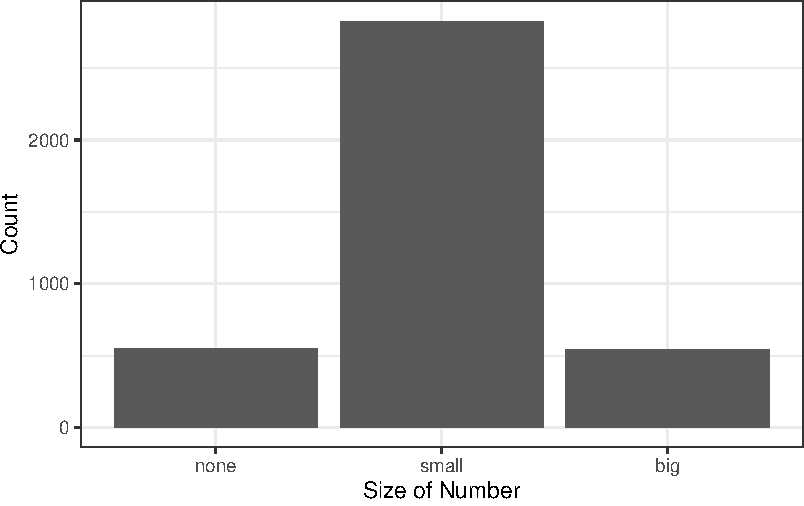
\includegraphics{06-Categorical-Data_files/figure-pdf/fig-bar61-1.pdf}

}

\caption{\label{fig-bar61}Bar chart of the \texttt{number} variable.}

\end{figure}%

Next, the counts are converted into proportions (e.g.,
\(549 / 3921 = 0.140\) for \texttt{none}) in Figure~\ref{fig-bar62}.

\begin{Shaded}
\begin{Highlighting}[]
\NormalTok{email }\SpecialCharTok{\%\textgreater{}\%}
  \FunctionTok{gf\_props}\NormalTok{(}\SpecialCharTok{\textasciitilde{}}\NormalTok{number) }\SpecialCharTok{\%\textgreater{}\%}
  \FunctionTok{gf\_theme}\NormalTok{(}\FunctionTok{theme\_bw}\NormalTok{()) }\SpecialCharTok{\%\textgreater{}\%}
  \FunctionTok{gf\_labs}\NormalTok{(}\AttributeTok{x =} \StringTok{"Size of Number"}\NormalTok{, }\AttributeTok{y =} \StringTok{"Proportion"}\NormalTok{)}
\end{Highlighting}
\end{Shaded}

\begin{figure}[H]

\centering{

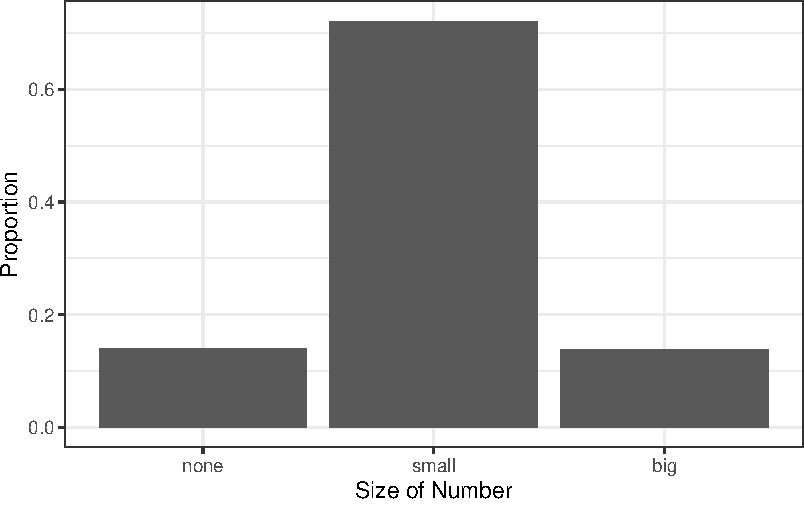
\includegraphics{06-Categorical-Data_files/figure-pdf/fig-bar62-1.pdf}

}

\caption{\label{fig-bar62}Bar chart of the \texttt{number} variable as a
proportion.}

\end{figure}%

Again, let's clean up the plot into a style that we could use in a
report.

\begin{Shaded}
\begin{Highlighting}[]
\NormalTok{email }\SpecialCharTok{\%\textgreater{}\%}
  \FunctionTok{gf\_props}\NormalTok{(}\SpecialCharTok{\textasciitilde{}}\NormalTok{number, }
           \AttributeTok{title =} \StringTok{"The proportions of emails with a number in it"}\NormalTok{,}
           \AttributeTok{subtitle =} \StringTok{"From 2012"}\NormalTok{, }\AttributeTok{xlab =} \StringTok{"Type of number in the email"}\NormalTok{,}
           \AttributeTok{ylab =} \StringTok{"Proportion of emails"}\NormalTok{) }\SpecialCharTok{\%\textgreater{}\%}
  \FunctionTok{gf\_theme}\NormalTok{(}\FunctionTok{theme\_bw}\NormalTok{())}
\end{Highlighting}
\end{Shaded}

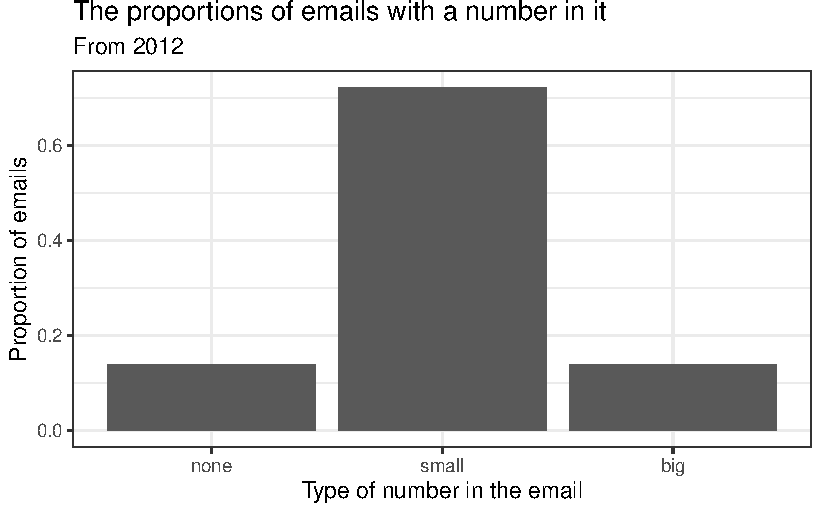
\includegraphics{06-Categorical-Data_files/figure-pdf/unnamed-chunk-16-1.pdf}

\subsection{Column proportions}\label{column-proportions}

The table below shows the column proportions. The \textbf{column
proportions} are computed as the counts divided by their column totals.
The value 149 at the intersection of \emph{spam} and \emph{none} is
replaced by \(149 / 549 = 0.271\), i.e., 149 divided by its column
total, 549. So what does 0.271 represent? It corresponds to the
proportion of emails in the sample with no numbers that are spam. That
is, the proportion of emails that are spam, out of all the emails with
no numbers. We are \textbf{conditioning}, restricting, on emails with no
number. This rate of spam is much higher than emails with only small
numbers (5.9\%) or big numbers (9.2\%). Because these spam rates vary
between the three levels of \texttt{number} (\emph{none}, \emph{small},
\emph{big}), this provides evidence that the \texttt{spam} and
\texttt{number} variables are associated.

\begin{Shaded}
\begin{Highlighting}[]
\FunctionTok{tally}\NormalTok{(spam }\SpecialCharTok{\textasciitilde{}}\NormalTok{ number, }\AttributeTok{data =}\NormalTok{ email, }\AttributeTok{margins =} \ConstantTok{TRUE}\NormalTok{, }\AttributeTok{format =} \StringTok{\textquotesingle{}proportion\textquotesingle{}}\NormalTok{)}
\end{Highlighting}
\end{Shaded}

\begin{verbatim}
          number
spam             none      small        big
  spam     0.27140255 0.05942695 0.09174312
  not spam 0.72859745 0.94057305 0.90825688
  Total    1.00000000 1.00000000 1.00000000
\end{verbatim}

The \texttt{tally()} function will always condition on the variable on
the right-hand side of the tilde, \textasciitilde, when calculating
proportions. Thus, \texttt{tally()} only generates column or overall
proportions. It cannot generate row proportions. The more general
\texttt{table()} function of \texttt{R} will allow either column or row
proportions.

\begin{quote}
\textbf{Exercise}:\\
Create a table of column proportions where the variable \texttt{spam} is
the column variable.
\end{quote}

\begin{Shaded}
\begin{Highlighting}[]
\FunctionTok{tally}\NormalTok{(number }\SpecialCharTok{\textasciitilde{}}\NormalTok{ spam, }\AttributeTok{data =}\NormalTok{ email, }\AttributeTok{margins =} \ConstantTok{TRUE}\NormalTok{, }\AttributeTok{format =} \StringTok{\textquotesingle{}proportion\textquotesingle{}}\NormalTok{)}
\end{Highlighting}
\end{Shaded}

\begin{verbatim}
       spam
number       spam  not spam
  none  0.4059946 0.1125492
  small 0.4577657 0.7481711
  big   0.1362398 0.1392797
  Total 1.0000000 1.0000000
\end{verbatim}

\begin{quote}
\textbf{Exercise}:\\
In the table you just created, what does 0.748 represent?\footnote{This
  is the proportion of \texttt{not\ spam} emails that had a small number
  in it.}
\end{quote}

\begin{quote}
\textbf{Exercise}: Create a table of proportions, where \texttt{spam} is
the column variable and the values shown represent the proportion of the
entire sample in each category.
\end{quote}

\begin{Shaded}
\begin{Highlighting}[]
\FunctionTok{tally}\NormalTok{(}\SpecialCharTok{\textasciitilde{}}\NormalTok{ number }\SpecialCharTok{+}\NormalTok{ spam, }\AttributeTok{data =}\NormalTok{ email, }\AttributeTok{margins =} \ConstantTok{TRUE}\NormalTok{, }\AttributeTok{format =} \StringTok{"proportion"}\NormalTok{)}
\end{Highlighting}
\end{Shaded}

\begin{verbatim}
       spam
number        spam   not spam      Total
  none  0.03800051 0.10201479 0.14001530
  small 0.04284621 0.67814333 0.72098954
  big   0.01275185 0.12624331 0.13899515
  Total 0.09359857 0.90640143 1.00000000
\end{verbatim}

\begin{quote}
\emph{Example}:\\
Data scientists use statistics to filter spam from incoming email
messages. By noting specific characteristics of an email, a data
scientist may be able to classify some emails as spam or not spam with
high accuracy. One of those characteristics is whether the email
contains no numbers, small numbers, or big numbers. Another
characteristic is whether or not an email has any HTML content (given by
the \texttt{format} variable). A contingency table for the \texttt{spam}
and \texttt{format} variables is needed.\\
1. Make \texttt{format} into a categorical factor variable. The levels
should be ``text'' and ``HTML''.\footnote{From the help menu on the
  data, HTML is coded as a 1.}\\
2. Create a contingency table from the \texttt{email} data set with
\texttt{format} in the columns and \texttt{spam} in the rows.
\end{quote}

\begin{Shaded}
\begin{Highlighting}[]
\NormalTok{email }\OtherTok{\textless{}{-}}\NormalTok{ email }\SpecialCharTok{\%\textgreater{}\%} 
  \FunctionTok{mutate}\NormalTok{(}\AttributeTok{format =} \FunctionTok{factor}\NormalTok{(email}\SpecialCharTok{$}\NormalTok{format, }\AttributeTok{levels =} \FunctionTok{c}\NormalTok{(}\DecValTok{1}\NormalTok{, }\DecValTok{0}\NormalTok{), }
                         \AttributeTok{labels =} \FunctionTok{c}\NormalTok{(}\StringTok{"HTML"}\NormalTok{, }\StringTok{"text"}\NormalTok{)))}
\end{Highlighting}
\end{Shaded}

In deciding which variable to use as a column, the data scientist would
be interested in how the proportion of spam changes within each email
format. This corresponds to column proportions based on \texttt{format}:
the proportion of spam in plain text emails and the proportion of spam
in HTML emails.

\begin{Shaded}
\begin{Highlighting}[]
\FunctionTok{tally}\NormalTok{(spam }\SpecialCharTok{\textasciitilde{}}\NormalTok{ format, }\AttributeTok{data =}\NormalTok{ email, }\AttributeTok{margins =} \ConstantTok{TRUE}\NormalTok{, }\AttributeTok{format =} \StringTok{"proportion"}\NormalTok{)}
\end{Highlighting}
\end{Shaded}

\begin{verbatim}
          format
spam             HTML       text
  spam     0.05796038 0.17489540
  not spam 0.94203962 0.82510460
  Total    1.00000000 1.00000000
\end{verbatim}

In generating the column proportions, we can see that a higher fraction
of plain text emails are spam (\(209 / 1195 = 17.5\%\)) compared to HTML
emails (\(158 / 2726 = 5.8\%\)). This information on its own is
insufficient to classify an email as spam or not spam, as over 80\% of
plain text emails are not spam. Yet, when we carefully combine this
information with many other characteristics, such as \texttt{number} and
other variables, we stand a reasonable chance of being able to classify
an email as spam or not spam.

In constructing a table, we need to think about which variable we want
in the column and which in the row. The formula notation in some ways
makes us think about the response and predictor variables, with the
response variable (left-hand side) displayed in the rows and the
predictor variable (right-hand side) displayed in the columns. However,
in some cases, it is not clear which variable should be in the column
and row and the analyst must decide what is being communicated with the
table. Before settling on one form for a table, it is important to
consider the audience and the message they are to receive from the
table.

\begin{quote}
\textbf{Exercise}:\\
Create two tables with \texttt{number} and \texttt{spam}: one where
\texttt{number} is in the columns, and one where \texttt{spam} is in the
columns. Which table would be more useful to someone hoping to identify
spam emails based on the type of numbers in the email?\footnote{The
  table with \texttt{number} in the columns will probably be most
  useful. This table makes it easier to see that emails with small
  numbers are spam about 5.9\% of the time (relatively rare). In
  contrast, we see that about 27.1\% of emails with no numbers are spam,
  and 9.2\% of emails with big numbers are spam.}
\end{quote}

\begin{Shaded}
\begin{Highlighting}[]
\FunctionTok{tally}\NormalTok{(spam }\SpecialCharTok{\textasciitilde{}}\NormalTok{ number, }\AttributeTok{data =}\NormalTok{ email, }\AttributeTok{format =} \StringTok{\textquotesingle{}proportion\textquotesingle{}}\NormalTok{, }\AttributeTok{margin =} \ConstantTok{TRUE}\NormalTok{)}
\end{Highlighting}
\end{Shaded}

\begin{verbatim}
          number
spam             none      small        big
  spam     0.27140255 0.05942695 0.09174312
  not spam 0.72859745 0.94057305 0.90825688
  Total    1.00000000 1.00000000 1.00000000
\end{verbatim}

\begin{Shaded}
\begin{Highlighting}[]
\FunctionTok{tally}\NormalTok{(number }\SpecialCharTok{\textasciitilde{}}\NormalTok{ spam, }\AttributeTok{data =}\NormalTok{ email, }\AttributeTok{format =} \StringTok{\textquotesingle{}proportion\textquotesingle{}}\NormalTok{, }\AttributeTok{margin =} \ConstantTok{TRUE}\NormalTok{)}
\end{Highlighting}
\end{Shaded}

\begin{verbatim}
       spam
number       spam  not spam
  none  0.4059946 0.1125492
  small 0.4577657 0.7481711
  big   0.1362398 0.1392797
  Total 1.0000000 1.0000000
\end{verbatim}

\subsection{Segmented bar and mosaic
plots}\label{segmented-bar-and-mosaic-plots}

Contingency tables using column proportions are especially useful for
examining how two categorical variables are related. Segmented bar and
mosaic plots provide a way to visualize the information in these tables.

A \textbf{segmented bar plot} is a graphical display of contingency
table information. For example, a segmented bar plot representing the
table with \texttt{number} in the columns is shown in
Figure~\ref{fig-barseg61}, where we have first created a bar plot using
the \texttt{number} variable and then separated each group by the levels
of \texttt{spam} using the \texttt{fill} argument.

\begin{Shaded}
\begin{Highlighting}[]
\NormalTok{email }\SpecialCharTok{\%\textgreater{}\%}
  \FunctionTok{gf\_bar}\NormalTok{(}\SpecialCharTok{\textasciitilde{}}\NormalTok{number, }\AttributeTok{fill =} \SpecialCharTok{\textasciitilde{}}\NormalTok{spam) }\SpecialCharTok{\%\textgreater{}\%}
  \FunctionTok{gf\_theme}\NormalTok{(}\FunctionTok{theme\_bw}\NormalTok{()) }\SpecialCharTok{\%\textgreater{}\%}
  \FunctionTok{gf\_labs}\NormalTok{(}\AttributeTok{x =} \StringTok{"Size of Number"}\NormalTok{, }\AttributeTok{y =} \StringTok{"Count"}\NormalTok{)}
\end{Highlighting}
\end{Shaded}

\begin{figure}[H]

\centering{

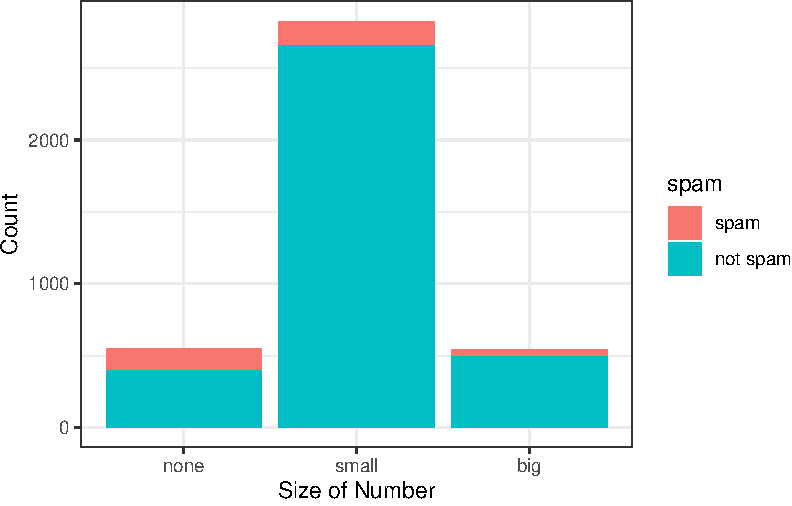
\includegraphics{06-Categorical-Data_files/figure-pdf/fig-barseg61-1.pdf}

}

\caption{\label{fig-barseg61}Segmented bar plot for numbers found in
\texttt{emails}, where the counts have been further broken down by
\texttt{spam}.}

\end{figure}%

The column proportions of the table have been translated into a
standardized segmented bar plot in Figure~\ref{fig-barseg62}, which is a
helpful visualization of the fraction of spam emails within each level
of \texttt{number}.

\begin{Shaded}
\begin{Highlighting}[]
\NormalTok{email }\SpecialCharTok{\%\textgreater{}\%}
  \FunctionTok{gf\_props}\NormalTok{(}\SpecialCharTok{\textasciitilde{}}\NormalTok{number, }\AttributeTok{fill =} \SpecialCharTok{\textasciitilde{}}\NormalTok{spam, }\AttributeTok{position =} \StringTok{\textquotesingle{}fill\textquotesingle{}}\NormalTok{) }\SpecialCharTok{\%\textgreater{}\%}
  \FunctionTok{gf\_theme}\NormalTok{(}\FunctionTok{theme\_bw}\NormalTok{()) }\SpecialCharTok{\%\textgreater{}\%}
  \FunctionTok{gf\_labs}\NormalTok{(}\AttributeTok{x =} \StringTok{"Size of Number"}\NormalTok{, }\AttributeTok{y =} \StringTok{"Proportion"}\NormalTok{)}
\end{Highlighting}
\end{Shaded}

\begin{figure}[H]

\centering{

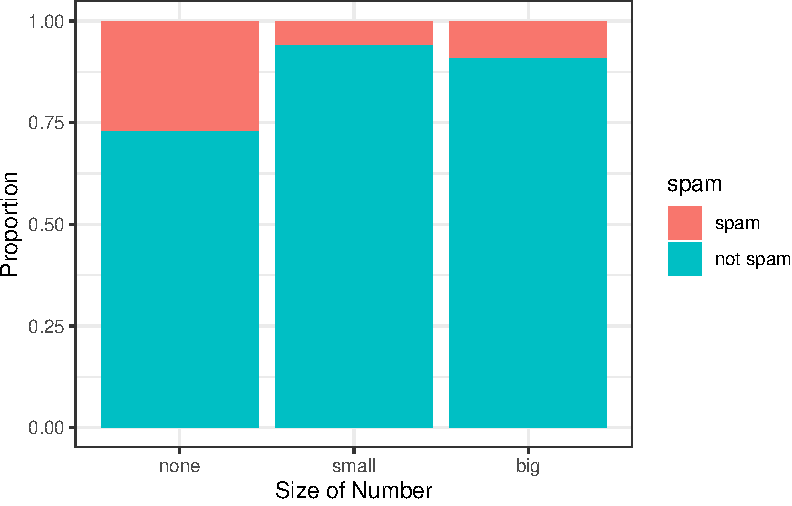
\includegraphics{06-Categorical-Data_files/figure-pdf/fig-barseg62-1.pdf}

}

\caption{\label{fig-barseg62}Standardized version of
Figure~\ref{fig-barseg61}.}

\end{figure}%

\begin{quote}
\emph{Example}:\\
Examine both of the segmented bar plots. Which is more
useful?\footnote{Figure~\ref{fig-barseg61} contains more information,
  but Figure~\ref{fig-barseg62} presents the information more clearly.
  This second plot makes it clear that emails with no number have a
  relatively high rate of spam email -- about 27\%! On the other hand,
  less than 10\% of emails with small or big numbers are spam.}
\end{quote}

Since the proportion of spam changes across the groups in
Figure~\ref{fig-barseg62}, we can conclude the variables are dependent,
which is something we were also able to discern using table proportions.
Because both the \texttt{none} and \texttt{big} groups have relatively
few observations compared to the \texttt{small} group, the association
is more difficult to see in Figure~\ref{fig-barseg61}.

In other cases, a segmented bar plot that is not standardized will be
more useful in communicating important information. Before settling on a
particular segmented bar plot, create standardized and non-standardized
forms and decide which is more effective at communicating features of
the data.

A \textbf{mosaic plot} is a graphical display of contingency table
information that is similar to a bar plot for one variable or a
segmented bar plot when using two variables. It seems strange, but
mosaic plots are not part of the \textbf{mosaic} package. We must load
another set of packages called \textbf{vcd} and \textbf{vcdExtra}.
Mosaic plots help to visualize the pattern of associations among
variables in two-way and larger tables. Mosaic plots are controversial
because they rely on the perception of area; human vision is not good at
distinguishing areas.

We introduce mosaic plots as another way to visualize contingency
tables. Figure~\ref{fig-mosaic61} shows a one-variable mosaic plot for
the \texttt{number} variable. Each row represents a level of
\texttt{number}, and the row heights correspond to the proportion of
emails of each number type. For instance, there are fewer emails with no
numbers than emails with only small numbers, so the \texttt{none}
outcome row is shorter in height. In general, mosaic plots use box
\emph{areas} to represent the number of observations. Since there is
only one variable, the widths are all constant. Thus area is simply
related to row height making this visual easy to read.

\begin{Shaded}
\begin{Highlighting}[]
\FunctionTok{library}\NormalTok{(vcd)}
\end{Highlighting}
\end{Shaded}

\begin{Shaded}
\begin{Highlighting}[]
\FunctionTok{mosaic}\NormalTok{(}\SpecialCharTok{\textasciitilde{}}\NormalTok{number, }\AttributeTok{data =}\NormalTok{ email)}
\end{Highlighting}
\end{Shaded}

\begin{figure}[H]

\centering{

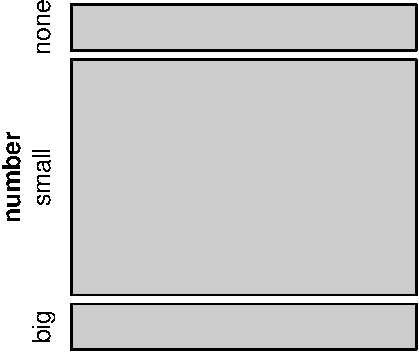
\includegraphics{06-Categorical-Data_files/figure-pdf/fig-mosaic61-1.pdf}

}

\caption{\label{fig-mosaic61}Mosaic plot where emails are grouped by the
\texttt{number} variable.}

\end{figure}%

This one-variable mosaic plot can be further divided into pieces as in
Figure~\ref{fig-mosaic62} using the \texttt{spam} variable. The first
variable in the formula is used to determine row height. That is, each
row is split proportionally according to the fraction of emails in each
number category. These heights are similar to those in
Figure~\ref{fig-mosaic61}. Next, each row is split horizontally
according to the proportion of emails that were spam in that number
group. For example, the second row, representing emails with only small
numbers, was divided into emails that were spam (left) and not spam
(right). The area of the rectangles represents the overall proportions
in the table, where each cell count is divided by the total count.
First, we will generate the table and then represent it as a mosaic
plot.

\begin{Shaded}
\begin{Highlighting}[]
\FunctionTok{tally}\NormalTok{(}\SpecialCharTok{\textasciitilde{}}\NormalTok{number }\SpecialCharTok{+}\NormalTok{ spam, }\AttributeTok{data =}\NormalTok{ email, }\AttributeTok{format =} \StringTok{\textquotesingle{}proportion\textquotesingle{}}\NormalTok{)}
\end{Highlighting}
\end{Shaded}

\begin{verbatim}
       spam
number        spam   not spam
  none  0.03800051 0.10201479
  small 0.04284621 0.67814333
  big   0.01275185 0.12624331
\end{verbatim}

\begin{Shaded}
\begin{Highlighting}[]
\FunctionTok{mosaic}\NormalTok{(}\SpecialCharTok{\textasciitilde{}}\NormalTok{number }\SpecialCharTok{+}\NormalTok{ spam, }\AttributeTok{data =}\NormalTok{ email)}
\end{Highlighting}
\end{Shaded}

\begin{figure}[H]

\centering{

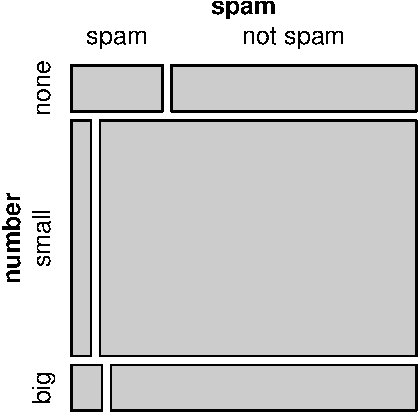
\includegraphics{06-Categorical-Data_files/figure-pdf/fig-mosaic62-1.pdf}

}

\caption{\label{fig-mosaic62}Mosaic plot with \texttt{number} as the
first (row) variable.}

\end{figure}%

These plots are hard to use in a visual comparison of area. For example,
is the area for \emph{small} number \emph{spam} emails different from
\emph{none} number \emph{spam} emails? The rectangles have different
shapes but from the table we can tell the areas are very similar.

An important use of the mosaic plot is to determine if an association
between variables may be present. The bottom row of the first column
represents spam emails that had big numbers, and the bottom row of the
second column represents regular emails that had big numbers. We can
again use this plot to see that the \texttt{spam} and \texttt{number}
variables are associated since some rows are divided in different
vertical locations than others, which was the same technique used for
checking an association in the standardized version of the segmented bar
plot.

In a similar way, a mosaic plot representing column proportions where
\emph{spam} is in the column could be constructed.

\begin{Shaded}
\begin{Highlighting}[]
\FunctionTok{mosaic}\NormalTok{(}\SpecialCharTok{\textasciitilde{}}\NormalTok{spam }\SpecialCharTok{+}\NormalTok{ number, }\AttributeTok{data =}\NormalTok{ email)}
\end{Highlighting}
\end{Shaded}

\begin{figure}[H]

\centering{

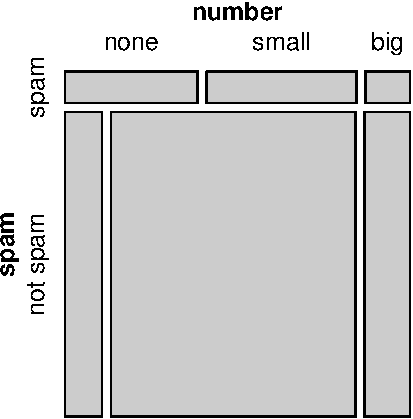
\includegraphics{06-Categorical-Data_files/figure-pdf/fig-mosaic63-1.pdf}

}

\caption{\label{fig-mosaic63}Mosaic plot with \texttt{spam} as the first
(row) variable.}

\end{figure}%

To completely understand the mosaic plot as shown in
Figure~\ref{fig-mosaic63}, let's first find the proportions of
\texttt{spam}.

\begin{Shaded}
\begin{Highlighting}[]
\FunctionTok{tally}\NormalTok{(}\SpecialCharTok{\textasciitilde{}}\NormalTok{spam, }\AttributeTok{data =}\NormalTok{ email, }\AttributeTok{format =} \StringTok{"proportion"}\NormalTok{)}
\end{Highlighting}
\end{Shaded}

\begin{verbatim}
spam
      spam   not spam 
0.09359857 0.90640143 
\end{verbatim}

So, the row heights will be split 90-10. Next, let's find the
proportions of \texttt{number} within each value of \texttt{spam}. In
the spam row, \emph{none} will be 41\%, \emph{small} will be 46\%, and
\emph{big} will be 13\%. In the not spam row, \emph{none} will be 11\%,
\emph{small} will be 75\%, and \emph{big} will be 14\%.

\begin{Shaded}
\begin{Highlighting}[]
\FunctionTok{tally}\NormalTok{(number }\SpecialCharTok{\textasciitilde{}}\NormalTok{ spam, }\AttributeTok{data =}\NormalTok{ email, }\AttributeTok{margins =} \ConstantTok{TRUE}\NormalTok{, }\AttributeTok{format =} \StringTok{"proportion"}\NormalTok{)}
\end{Highlighting}
\end{Shaded}

\begin{verbatim}
       spam
number       spam  not spam
  none  0.4059946 0.1125492
  small 0.4577657 0.7481711
  big   0.1362398 0.1392797
  Total 1.0000000 1.0000000
\end{verbatim}

However, because it is more insightful for this application to consider
the fraction of spam in each category of the \texttt{number} variable,
we prefer Figure~\ref{fig-mosaic62}.

\subsection{The only pie chart you will see in this book,
hopefully}\label{the-only-pie-chart-you-will-see-in-this-book-hopefully}

While pie charts are well known, they are typically not as useful as
other charts in a data analysis. A \textbf{pie chart} is shown in
Figure~\ref{fig-pie61}. It is generally more difficult to compare group
sizes in a pie chart than in a bar plot, especially when categories have
nearly identical counts or proportions. Just as human vision is bad at
distinguishing areas, human vision is also bad at distinguishing angles.
In the case of the \emph{none} and \emph{big} categories, the difference
is so slight you may be unable to distinguish any difference in group
sizes.

\begin{Shaded}
\begin{Highlighting}[]
\FunctionTok{pie}\NormalTok{(}\FunctionTok{table}\NormalTok{(email}\SpecialCharTok{$}\NormalTok{number), }\AttributeTok{col =}\NormalTok{ COL[}\FunctionTok{c}\NormalTok{(}\DecValTok{3}\NormalTok{, }\DecValTok{1}\NormalTok{, }\DecValTok{2}\NormalTok{)], }\AttributeTok{radius =} \FloatTok{0.75}\NormalTok{)}
\end{Highlighting}
\end{Shaded}

\begin{figure}[H]

\centering{

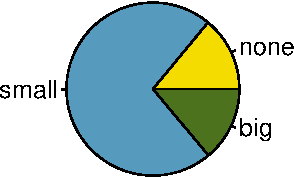
\includegraphics{06-Categorical-Data_files/figure-pdf/fig-pie61-1.pdf}

}

\caption{\label{fig-pie61}A pie chart for \texttt{number} in the email
data set.}

\end{figure}%

Pie charts are popular in the Air Force due to the ease of generating
them in Excel and PowerPoint. However, the values for each slice are
often printed on top of the chart making the chart irrelevant. We
recommend a minimal use of pie charts in your work.

\subsection{Comparing numerical data across
groups}\label{comparing-numerical-data-across-groups}

Some of the more interesting investigations can be done by examining
numerical data across groups. This is the case where one variable is
categorical and the other is numerical. The methods required here aren't
really new. All that is required is to make a numerical plot for each
group. Here, two convenient methods are introduced: side-by-side box
plots and density plots.

We will again take a look at the subset of the \texttt{county\_complete}
data set. Let's compare the median household income for counties that
gained population from 2000 to 2010 versus counties that had no gain.
While we might like to make a causal connection here, remember that
these are observational data, so such an interpretation would be
unjustified.

This section will give us a chance to perform some data wrangling. We
will be using the \texttt{tidyverse} verbs in the process. Data
wrangling is an important part of analysis work and typically makes up a
significant portion of the analysis work.

Here is the code to generate the data we need.

\begin{Shaded}
\begin{Highlighting}[]
\FunctionTok{library}\NormalTok{(usdata)}
\end{Highlighting}
\end{Shaded}

\begin{Shaded}
\begin{Highlighting}[]
\NormalTok{county\_tidy }\OtherTok{\textless{}{-}}\NormalTok{ county\_complete }\SpecialCharTok{\%\textgreater{}\%} 
  \FunctionTok{select}\NormalTok{(name, state, pop2000, pop2010, }\AttributeTok{fed\_spend =}\NormalTok{ fed\_spending\_2009, }
         \AttributeTok{poverty =}\NormalTok{ poverty\_2010, }\AttributeTok{homeownership =}\NormalTok{ homeownership\_2010, }
         \AttributeTok{multi\_unit =}\NormalTok{ housing\_multi\_unit\_2010, }\AttributeTok{income =}\NormalTok{ per\_capita\_income\_2010, }
         \AttributeTok{med\_income =}\NormalTok{ median\_household\_income\_2010) }\SpecialCharTok{\%\textgreater{}\%}
  \FunctionTok{mutate}\NormalTok{(}\AttributeTok{fed\_spend =}\NormalTok{ fed\_spend }\SpecialCharTok{/}\NormalTok{ pop2010)}
\end{Highlighting}
\end{Shaded}

First, as a reminder, let's look at the data.

\emph{What do we want \texttt{R} to do?}

We want to select the variables \texttt{pop2000}, \texttt{pop2010}, and
\texttt{med\_income}.

\emph{What does \texttt{R} need in order to do this?}

It needs the data object, and the desired variable names.

We will use the \texttt{select()} and \texttt{inspect()} functions.

\begin{Shaded}
\begin{Highlighting}[]
\NormalTok{county\_tidy }\SpecialCharTok{\%\textgreater{}\%}
  \FunctionTok{select}\NormalTok{(pop2000, pop2010, med\_income) }\SpecialCharTok{\%\textgreater{}\%}
  \FunctionTok{inspect}\NormalTok{()}
\end{Highlighting}
\end{Shaded}

\begin{verbatim}

quantitative variables:  
        name   class   min       Q1 median    Q3     max     mean        sd
1    pop2000 numeric    67 11223.50  24621 61775 9519338 89649.99 292547.67
2    pop2010 numeric    82 11114.50  25872 66780 9818605 98262.04 312946.70
3 med_income numeric 19351 36956.25  42450 49144  115574 44274.12  11547.49
     n missing
1 3139       3
2 3142       0
3 3142       0
\end{verbatim}

Notice that three counties are missing population values for the year
2000, reported as \texttt{NA}. Let's remove them and find which counties
increased in population by creating a new variable.

\begin{Shaded}
\begin{Highlighting}[]
\NormalTok{cc\_reduced }\OtherTok{\textless{}{-}}\NormalTok{ county\_tidy }\SpecialCharTok{\%\textgreater{}\%}
  \FunctionTok{drop\_na}\NormalTok{(pop2000) }\SpecialCharTok{\%\textgreater{}\%}
  \FunctionTok{select}\NormalTok{(pop2000, pop2010, med\_income) }\SpecialCharTok{\%\textgreater{}\%}
  \FunctionTok{mutate}\NormalTok{(}\AttributeTok{pop\_gain =} \FunctionTok{sign}\NormalTok{(pop2010}\SpecialCharTok{{-}}\NormalTok{pop2000))}
\end{Highlighting}
\end{Shaded}

\begin{Shaded}
\begin{Highlighting}[]
\FunctionTok{tally}\NormalTok{(}\SpecialCharTok{\textasciitilde{}}\NormalTok{pop\_gain, }\AttributeTok{data =}\NormalTok{ cc\_reduced)}
\end{Highlighting}
\end{Shaded}

\begin{verbatim}
pop_gain
  -1    0    1 
1097    1 2041 
\end{verbatim}

There were 2,041 counties where the population increased from 2000 to
2010, and there were 1,098 counties with no gain. Only 1 county had a
net of zero, and 1,0987 had a loss. Let's just look at the counties with
a gain or loss in a side-by-side boxplot. Again, we will use
\texttt{filter()} to select the two groups and then make the variable
\texttt{pop\_gain} into a categorical variable. It's time for more data
wrangling.

\begin{Shaded}
\begin{Highlighting}[]
\NormalTok{cc\_reduced }\OtherTok{\textless{}{-}}\NormalTok{ cc\_reduced }\SpecialCharTok{\%\textgreater{}\%}
  \FunctionTok{filter}\NormalTok{(pop\_gain }\SpecialCharTok{!=} \DecValTok{0}\NormalTok{) }\SpecialCharTok{\%\textgreater{}\%}
  \FunctionTok{mutate}\NormalTok{(}\AttributeTok{pop\_gain =} \FunctionTok{factor}\NormalTok{(pop\_gain, }\AttributeTok{levels =} \FunctionTok{c}\NormalTok{(}\SpecialCharTok{{-}}\DecValTok{1}\NormalTok{, }\DecValTok{1}\NormalTok{), }
                           \AttributeTok{labels =} \FunctionTok{c}\NormalTok{(}\StringTok{"Loss"}\NormalTok{, }\StringTok{"Gain"}\NormalTok{)))}
\end{Highlighting}
\end{Shaded}

\begin{Shaded}
\begin{Highlighting}[]
\FunctionTok{inspect}\NormalTok{(cc\_reduced)}
\end{Highlighting}
\end{Shaded}

\begin{verbatim}

categorical variables:  
      name  class levels    n missing
1 pop_gain factor      2 3138       0
                                   distribution
1 Gain (65%), Loss (35%)                       

quantitative variables:  
        name   class   min       Q1  median      Q3     max     mean        sd
1    pop2000 numeric    67 11217.25 24608.0 61783.5 9519338 89669.37 292592.28
2    pop2010 numeric    82 11127.00 25872.0 66972.0 9818605 98359.23 313133.28
3 med_income numeric 19351 36950.00 42443.5 49120.0  115574 44253.24  11528.95
     n missing
1 3138       0
2 3138       0
3 3138       0
\end{verbatim}

The \textbf{side-by-side box plot} is a traditional tool for comparing
across groups. An example is shown in Figure~\ref{fig-sbysbox61} where
there are two box plots, one for each group, drawn on the same scale.

\begin{Shaded}
\begin{Highlighting}[]
\NormalTok{cc\_reduced }\SpecialCharTok{\%\textgreater{}\%}
  \FunctionTok{gf\_boxplot}\NormalTok{(med\_income }\SpecialCharTok{\textasciitilde{}}\NormalTok{ pop\_gain,}
             \AttributeTok{subtitle =} \StringTok{"The income data were collected between 2006 and 2010."}\NormalTok{,}
             \AttributeTok{xlab =} \StringTok{"Population change from 2000 to 2010"}\NormalTok{,}
             \AttributeTok{ylab =} \StringTok{"Median Household Income"}\NormalTok{) }\SpecialCharTok{\%\textgreater{}\%}
  \FunctionTok{gf\_theme}\NormalTok{(}\FunctionTok{theme\_bw}\NormalTok{())}
\end{Highlighting}
\end{Shaded}

\begin{figure}[H]

\centering{

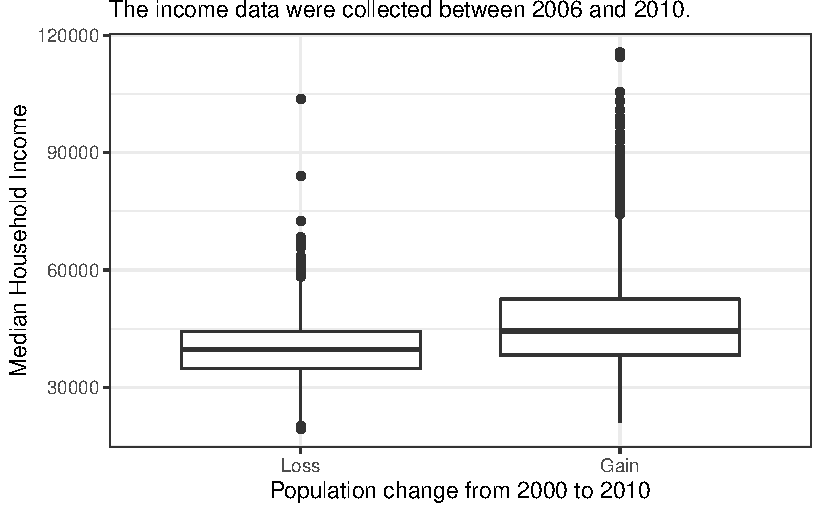
\includegraphics{06-Categorical-Data_files/figure-pdf/fig-sbysbox61-1.pdf}

}

\caption{\label{fig-sbysbox61}Side-by-side box plot for median household
income, where the counties are split by whether there was a population
gain or loss from 2000 to 2010.}

\end{figure}%

Another useful plotting method uses \textbf{density plots} to compare
numerical data across groups. A histogram bins data but is highly
dependent on the number and boundary of the bins. A density plot also
estimates the distribution of a numerical variable but does this by
estimating the density of data points in a small window around each data
point. The overall curve is the sum of this small density estimate. A
density plot can be thought of as a smooth version of the histogram.
Several options go into a density estimate, such as the width of the
window and type of smoothing function. These ideas are beyond the scope
here and we will just use the default options. Figure~\ref{fig-dens61}
is a plot of the two density curves.

\begin{Shaded}
\begin{Highlighting}[]
\NormalTok{cc\_reduced }\SpecialCharTok{\%\textgreater{}\%}
  \FunctionTok{gf\_dens}\NormalTok{(}\SpecialCharTok{\textasciitilde{}}\NormalTok{med\_income, }\AttributeTok{color =} \SpecialCharTok{\textasciitilde{}}\NormalTok{pop\_gain, }\AttributeTok{lwd =} \DecValTok{1}\NormalTok{) }\SpecialCharTok{\%\textgreater{}\%}
  \FunctionTok{gf\_theme}\NormalTok{(}\FunctionTok{theme\_bw}\NormalTok{()) }\SpecialCharTok{\%\textgreater{}\%}
  \FunctionTok{gf\_labs}\NormalTok{(}\AttributeTok{x =} \StringTok{"Median household income"}\NormalTok{, }\AttributeTok{y =} \StringTok{"Density"}\NormalTok{, }\AttributeTok{col =} \StringTok{"Population }\SpecialCharTok{\textbackslash{}n}\StringTok{Change"}\NormalTok{)}
\end{Highlighting}
\end{Shaded}

\begin{figure}[H]

\centering{

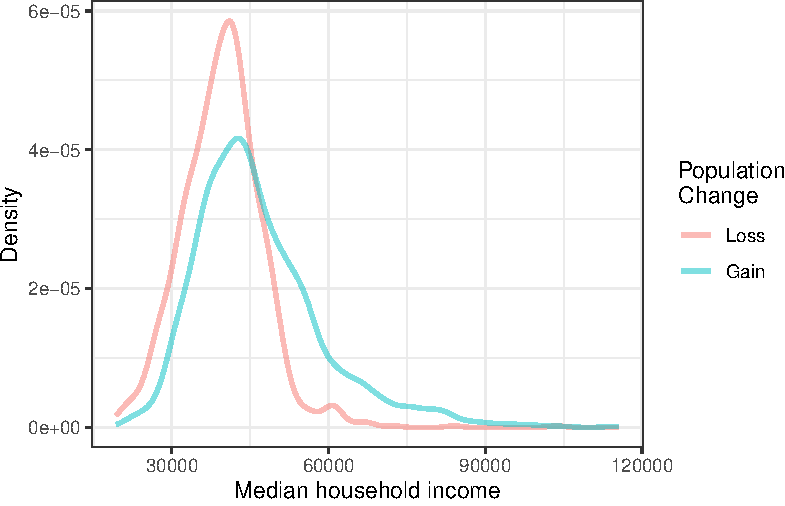
\includegraphics{06-Categorical-Data_files/figure-pdf/fig-dens61-1.pdf}

}

\caption{\label{fig-dens61}Density plots of median household income for
counties with population gain versus population loss.}

\end{figure}%

\begin{quote}
\textbf{Exercise}:\\
Use the box plots and density plots to compare the incomes for counties
across the two groups. What do you notice about the approximate center
of each group? What do you notice about the variability between groups?
Is the shape relatively consistent between groups? How many
\emph{prominent} modes are there for each group?\footnote{Answers may
  vary a little. The counties with population gains tend to have higher
  income (median of about \$45,000) versus counties without a gain
  (median of about \$40,000). The variability is also slightly larger
  for the population gain group. This is evident in the IQR, which is
  about 50\% bigger in the \emph{gain} group. Both distributions show
  slight to moderate right skew and are unimodal. There is a secondary
  small bump at about \$60,000 for the \emph{no gain} group, visible in
  the density plot, that seems out of place. (Looking into the data set,
  we would find that 8 of these 15 counties are in Alaska and Texas.)
  The box plots indicate there are many observations far above the
  median in each group, though we should anticipate that many
  observations will fall beyond the whiskers when using such a large
  data set.}
\end{quote}

\begin{quote}
\textbf{Exercise}:\\
What components of Figures~\ref{fig-sbysbox61}, \ref{fig-dens61} do you
find most useful?\footnote{The side-by-side box plots are especially
  useful for comparing centers and spreads, while the density plots are
  more useful for seeing distribution shape, skew, and groups of
  anomalies.}
\end{quote}

\section{Homework Problems}\label{homework-problems-5}

Create an Rmd file for the work including headers, file creation data,
and explanation of your work. Make sure your plots have a title and the
axes are labeled.

\begin{enumerate}
\def\labelenumi{\arabic{enumi}.}
\item
  \textbf{Views on immigration}. 910 randomly sampled, registered voters
  from Tampa, FL were asked if they thought workers who have illegally
  entered the US should be (i) allowed to keep their jobs and apply for
  US citizenship, (ii) allowed to keep their jobs as temporary guest
  workers but not allowed to apply for US citizenship, or (iii) lose
  their jobs and have to leave the country.

  The data is in the \textbf{openintro} package in the
  \texttt{immigration} data set.
\end{enumerate}

\begin{enumerate}
\def\labelenumi{\alph{enumi}.}
\item
  How many levels of \emph{political} are there?
\item
  Create a table using \texttt{tally()}. Note: a table showing overall
  proportions or percents may be most helpful for parts c) through e).
\item
  What percent of these Tampa, FL voters identify themselves as
  conservatives?
\item
  What percent of these Tampa, FL voters are in favor of the citizenship
  option?
\item
  What percent of these Tampa, FL voters identify themselves as
  conservatives and are in favor of the citizenship option?
\item
  What percent of these Tampa, FL voters who identify themselves as
  conservatives are also in favor of the citizenship option? What
  percent of moderates and liberal share this view?
\item
  Create a stacked bar chart to reflect your work in part f).
\item
  Using your plot, do political ideology and views on immigration appear
  to be independent? Explain your reasoning.
\end{enumerate}

\begin{enumerate}
\def\labelenumi{\arabic{enumi}.}
\setcounter{enumi}{1}
\item
  \textbf{Views on the DREAM Act}. The same survey from Exercise 1 also
  asked respondents if they support the DREAM Act, a proposed law which
  would provide a path to citizenship for people brought illegally to
  the US as children.

  The data is in the \textbf{openintro} package in the \texttt{dream}
  data object.
\end{enumerate}

\begin{enumerate}
\def\labelenumi{\alph{enumi}.}
\item
  Create a \emph{mosaic} plot of political view versus stance on the
  DREAM Act.
\item
  Based on the mosaic plot, are views on the DREAM Act and political
  ideology independent?
\end{enumerate}

\begin{enumerate}
\def\labelenumi{\arabic{enumi}.}
\setcounter{enumi}{2}
\item
  \textbf{Heart transplants}. The Stanford University Heart Transplant
  Study was conducted to determine whether an experimental heart
  transplant program increased lifespan. Each patient entering the
  program was designated an official heart transplant candidate, meaning
  that he was gravely ill and would most likely benefit from a new
  heart. Some patients got a transplant and some did not. The variable
  \emph{transplant} indicates which group the patients were in; patients
  in the treatment group got a transplant and those in the control group
  did not. Another variable called \emph{survived} was used to indicate
  whether or not the patient was alive at the end of the study.

  The data is in the \textbf{openintro} package and is called
  \texttt{heart\_transplant}.
\end{enumerate}

\begin{enumerate}
\def\labelenumi{\alph{enumi}.}
\item
  Create a \textbf{mosaic} plot of treatment versus survival status.
\item
  Based on the mosaic plot, is survival independent of whether or not
  the patient got a transplant? Explain your reasoning.
\item
  Create side-by-side boxplots of survival time for the control and
  treatment groups.
\item
  What do the box plots suggest about the efficacy (effectiveness) of
  transplants?
\end{enumerate}

\section*{\texorpdfstring{\href{https://ds-usafa.github.io/CPS-Solutions-Manual/CATDATA.html}{Solutions
Manual}}{Solutions Manual}}\label{solutions-manual-6}
\addcontentsline{toc}{section}{\href{https://ds-usafa.github.io/CPS-Solutions-Manual/CATDATA.html}{Solutions
Manual}}

\markright{Solutions Manual}

\part{Probability Modeling}

\chapter{Probability Case Study}\label{CS2}

\section{Objectives}\label{objectives-7}

\begin{enumerate}
\def\labelenumi{\arabic{enumi})}
\item
  Use \texttt{R} to simulate a probabilistic model.
\item
  Use basic counting methods.
\end{enumerate}

\section{Introduction to probability
models}\label{introduction-to-probability-models}

In this second block of material we will focus on probability models. We
will take two approaches, one is mathematical and the other is
computational. In some cases we can use both methods on a problem and in
others only the computational approach is feasible. The mathematical
approach to probability modeling allows us insight into the problem and
the ability to understand the process. Simulation has a much greater
ability to generalize but can be time intensive to run and often
requires the writing of custom functions.

This case study is extensive and may seem overwhelming, but do not
worry. We will discuss these ideas again in the many chapters we have
coming up this block.

\section{Probability models}\label{probability-models}

Probability models are an important tool for data analysts. They are
used to explain variation in outcomes that cannot be explained by other
variables. We will use these ideas in the Statistical Modeling Block to
help us make decisions about our statistical models.

Often probability models are used to answer a question of the form
``What is the chance that \ldots..?'' This means that we typically have
an experiment or trial where multiple outcomes are possible and we only
have an idea of the frequency of those outcomes. We use this frequency
as a measure of the probability of a particular outcome.

For this block we will focus just on probability models. To apply a
probability model we will need to

\begin{enumerate}
\def\labelenumi{\arabic{enumi}.}
\tightlist
\item
  Select the experiment and its possible outcomes.
\item
  Have probability values for the outcomes which may include
  \textbf{parameters} that determine the probabilities.
\item
  Understand the assumptions behind the model.
\end{enumerate}

\section{Case study}\label{case-study-1}

There is a famous example of a probability question that we will attack
in this case study. The question we want to answer is ``In a room of
\(n\) people what is the chance that at least two people have the same
birthday?''

\begin{quote}
\textbf{Exercise}:\\
The typical classroom at USAFA has 18 students in it. What do you think
the chance that at least two students have the same birthday?\footnote{The
  answer is around 34.7\%, how close were you?}
\end{quote}

\subsection{Break down the question}\label{break-down-the-question}

The first action we should take is to understand what is being asked.

\begin{enumerate}
\def\labelenumi{\arabic{enumi}.}
\tightlist
\item
  What is the experiment or trial?
\item
  What does it mean to have the same birthday?
\item
  What about leap years?
\item
  What about the frequency of births? Are some days less likely than
  others?
\end{enumerate}

\begin{quote}
\textbf{Exercise}:\\
Discuss these questions and others that you think are
relevant.\footnote{Another question may be What does it mean at least
  two people have matching birthdays?}
\end{quote}

The best first step is to make a simple model, often these are the only
ones that will have a mathematical solution. For our problem this means
we answer the above questions.

\begin{enumerate}
\def\labelenumi{\arabic{enumi}.}
\tightlist
\item
  We have a room of 18 people and we look at their birthdays. We either
  have two or more birthdays matching or not; thus there are two
  outcomes.
\item
  We don't care about the year, only the day and month. Thus two people
  born on May 16th are a match.
\item
  We will ignore leap years.
\item
  We will assume that a person has equal probability of being born on
  any of the 365 days of the year.
\item
  At least two means we could have multiple matches on the same day or
  several different days where multiple people have matching birthdays.
\end{enumerate}

\subsection{Simulate (computational)}\label{simulate-computational}

Now that we have an idea about the structure of the problem, we next
need to think about how we would simulate a single classroom. We have 18
students in the classroom and they all could have any of the 365 days of
the year as a birthday. What we need to do is sample birthdays for each
of the 18 students. But how do we code the days of the year?

An easy solution is to just label the days from 1 to 365. The function
\texttt{seq()} does this for us.

\begin{Shaded}
\begin{Highlighting}[]
\NormalTok{days }\OtherTok{\textless{}{-}} \FunctionTok{seq}\NormalTok{(}\DecValTok{1}\NormalTok{,}\DecValTok{365}\NormalTok{)}
\end{Highlighting}
\end{Shaded}

Next we need to pick one of the days using the sample function. Note
that we set the seed to get repeatable results, this is not required.

\begin{Shaded}
\begin{Highlighting}[]
\FunctionTok{set.seed}\NormalTok{(}\DecValTok{2022}\NormalTok{)}
\FunctionTok{sample}\NormalTok{(days,}\DecValTok{1}\NormalTok{)}
\end{Highlighting}
\end{Shaded}

\begin{verbatim}
[1] 228
\end{verbatim}

The first person was born on the 228th day of the year.

Since \texttt{R} works on vectors, we don't have to write a loop to
select 18 days, we just have \texttt{sample()} do it for us.

\begin{Shaded}
\begin{Highlighting}[]
\NormalTok{class }\OtherTok{\textless{}{-}} \FunctionTok{sample}\NormalTok{(days,}\AttributeTok{size=}\DecValTok{18}\NormalTok{,}\AttributeTok{replace =} \ConstantTok{TRUE}\NormalTok{)}
\NormalTok{class}
\end{Highlighting}
\end{Shaded}

\begin{verbatim}
 [1] 206 311 331 196 262 191 206 123 233 270 248   7 349 112   1 307 288 354
\end{verbatim}

What do we want \texttt{R} to do? Sample from the numbers 1 to 365 with
replacement, which means a number can be picked more than once.

Notice in our sample we have at least one match, although it is
difficult to look at this list and see the match. Let's sort them to
make it easier for us to see.

\begin{Shaded}
\begin{Highlighting}[]
\FunctionTok{sort}\NormalTok{(class)}
\end{Highlighting}
\end{Shaded}

\begin{verbatim}
 [1]   1   7 112 123 191 196 206 206 233 248 262 270 288 307 311 331 349 354
\end{verbatim}

The next step is to find a way in \texttt{R} for the code to detect that
there is a match.

\begin{quote}
\textbf{Exercise}:\\
What idea(s) can we use to determine if a match exists?
\end{quote}

We could sort the data and look at differences in sequential values and
then check if the set of differences contains a zero. This seems to be
computationally expensive. Instead we will use the function
\texttt{unique()} which gives a vector of unique values in an object.
The function \texttt{length()} gives the number of elements in the
vector.

\begin{Shaded}
\begin{Highlighting}[]
\FunctionTok{length}\NormalTok{(}\FunctionTok{unique}\NormalTok{(class))}
\end{Highlighting}
\end{Shaded}

\begin{verbatim}
[1] 17
\end{verbatim}

Since we only have 17 unique values in a vector of size 18, we have a
match. Now let's put this all together to generate another classroom of
size 18.

\begin{Shaded}
\begin{Highlighting}[]
\FunctionTok{length}\NormalTok{(}\FunctionTok{unique}\NormalTok{(}\FunctionTok{sample}\NormalTok{(days,}\AttributeTok{size=}\DecValTok{18}\NormalTok{,}\AttributeTok{replace =} \ConstantTok{TRUE}\NormalTok{)))}
\end{Highlighting}
\end{Shaded}

\begin{verbatim}
[1] 16
\end{verbatim}

The next problem that needs to be solved is how to repeat the classrooms
and keep track of those that have a match. There are several functions
we could use to include \texttt{replicate()} but we will use
\texttt{do()} from the \textbf{mosaic} package because it returns a data
frame so we can use \texttt{tidyverse} verbs to wrangle the data.

The \texttt{do()} function allows us to repeat an operation many times.
The following template

\begin{verbatim}
do(n) * {stuff to do}              # pseudo-code
\end{verbatim}

where \{stuff to do\} is typically a single \texttt{R} command, but may
be something more complicated.

Load the libraries.

\begin{Shaded}
\begin{Highlighting}[]
\FunctionTok{library}\NormalTok{(mosaic)}
\FunctionTok{library}\NormalTok{(tidyverse)}
\end{Highlighting}
\end{Shaded}

\begin{Shaded}
\begin{Highlighting}[]
\FunctionTok{do}\NormalTok{(}\DecValTok{5}\NormalTok{)}\SpecialCharTok{*}\FunctionTok{length}\NormalTok{(}\FunctionTok{unique}\NormalTok{(}\FunctionTok{sample}\NormalTok{(days,}\AttributeTok{size=}\DecValTok{18}\NormalTok{,}\AttributeTok{replace =} \ConstantTok{TRUE}\NormalTok{)))}
\end{Highlighting}
\end{Shaded}

\begin{verbatim}
  length
1     18
2     17
3     17
4     17
5     18
\end{verbatim}

Let's repeat for a larger number of simulated classroom, remember you
should be asking yourself:

\emph{What do I want \texttt{R} to do?}\\
\emph{What does \texttt{R} need to do this?}

\begin{Shaded}
\begin{Highlighting}[]
\NormalTok{(}\FunctionTok{do}\NormalTok{(}\DecValTok{1000}\NormalTok{)}\SpecialCharTok{*}\FunctionTok{length}\NormalTok{(}\FunctionTok{unique}\NormalTok{(}\FunctionTok{sample}\NormalTok{(days,}\AttributeTok{size=}\DecValTok{18}\NormalTok{,}\AttributeTok{replace =} \ConstantTok{TRUE}\NormalTok{)))) }\SpecialCharTok{\%\textgreater{}\%}
  \FunctionTok{mutate}\NormalTok{(}\AttributeTok{match=}\FunctionTok{if\_else}\NormalTok{(length}\SpecialCharTok{==}\DecValTok{18}\NormalTok{,}\DecValTok{0}\NormalTok{,}\DecValTok{1}\NormalTok{)) }\SpecialCharTok{\%\textgreater{}\%}
  \FunctionTok{summarise}\NormalTok{(}\AttributeTok{prob=}\FunctionTok{mean}\NormalTok{(match))}
\end{Highlighting}
\end{Shaded}

\begin{verbatim}
  prob
1 0.36
\end{verbatim}

This is within 2 decimal places of the mathematical solution we develop
shortly.

How many classrooms do we need to simulate to get an accurate estimate
of the probability of a match? That is a statistical modeling question
and it depends on how much variability we can accept. We will discuss
these ideas later in the book. For now, you can run the code multiple
times and see how the estimate varies. If computational power is cheap,
you can increase the number of simulations.

\begin{Shaded}
\begin{Highlighting}[]
\NormalTok{(}\FunctionTok{do}\NormalTok{(}\DecValTok{10000}\NormalTok{)}\SpecialCharTok{*}\FunctionTok{length}\NormalTok{(}\FunctionTok{unique}\NormalTok{(}\FunctionTok{sample}\NormalTok{(days,}\AttributeTok{size=}\DecValTok{18}\NormalTok{,}\AttributeTok{replace =} \ConstantTok{TRUE}\NormalTok{)))) }\SpecialCharTok{\%\textgreater{}\%}
  \FunctionTok{mutate}\NormalTok{(}\AttributeTok{match=}\FunctionTok{if\_else}\NormalTok{(length}\SpecialCharTok{==}\DecValTok{18}\NormalTok{,}\DecValTok{0}\NormalTok{,}\DecValTok{1}\NormalTok{)) }\SpecialCharTok{\%\textgreater{}\%}
  \FunctionTok{summarise}\NormalTok{(}\AttributeTok{prob=}\FunctionTok{mean}\NormalTok{(match))}
\end{Highlighting}
\end{Shaded}

\begin{verbatim}
    prob
1 0.3442
\end{verbatim}

\subsection{Plotting}\label{plotting}

By the way, the method we have used to create the data allows us to
summarize the number of unique birthdays using a table or bar chart.
Let's do that now. Note that since the first argument in
\texttt{tally()} is not data then the \textbf{pipe} operator will not
work without some extra effort. We must tell \texttt{R} that the data is
the previous argument in the pipeline and thus use the symbol \textbf{.}
to denote this.

\begin{Shaded}
\begin{Highlighting}[]
\NormalTok{(}\FunctionTok{do}\NormalTok{(}\DecValTok{1000}\NormalTok{)}\SpecialCharTok{*}\FunctionTok{length}\NormalTok{(}\FunctionTok{unique}\NormalTok{(}\FunctionTok{sample}\NormalTok{(days,}\AttributeTok{size=}\DecValTok{18}\NormalTok{,}\AttributeTok{replace =} \ConstantTok{TRUE}\NormalTok{)))) }\SpecialCharTok{\%\textgreater{}\%}
  \FunctionTok{tally}\NormalTok{(}\SpecialCharTok{\textasciitilde{}}\NormalTok{length,}\AttributeTok{data=}\NormalTok{.)}
\end{Highlighting}
\end{Shaded}

\begin{verbatim}
length
 14  15  16  17  18 
  1   7  52 253 687 
\end{verbatim}

Figure~\ref{fig-bar71} is a plot of the number of unique birthdays in
our sample.

\begin{Shaded}
\begin{Highlighting}[]
\NormalTok{(}\FunctionTok{do}\NormalTok{(}\DecValTok{1000}\NormalTok{)}\SpecialCharTok{*}\FunctionTok{length}\NormalTok{(}\FunctionTok{unique}\NormalTok{(}\FunctionTok{sample}\NormalTok{(days,}\AttributeTok{size=}\DecValTok{18}\NormalTok{,}\AttributeTok{replace =} \ConstantTok{TRUE}\NormalTok{)))) }\SpecialCharTok{\%\textgreater{}\%}
  \FunctionTok{gf\_bar}\NormalTok{(}\SpecialCharTok{\textasciitilde{}}\NormalTok{length) }\SpecialCharTok{\%\textgreater{}\%}
  \FunctionTok{gf\_theme}\NormalTok{(}\FunctionTok{theme\_bw}\NormalTok{()) }\SpecialCharTok{\%\textgreater{}\%}
  \FunctionTok{gf\_labs}\NormalTok{(}\AttributeTok{x=}\StringTok{"Number of unique birthdays"}\NormalTok{,}\AttributeTok{y=}\StringTok{"Count"}\NormalTok{)}
\end{Highlighting}
\end{Shaded}

\begin{figure}[H]

\centering{

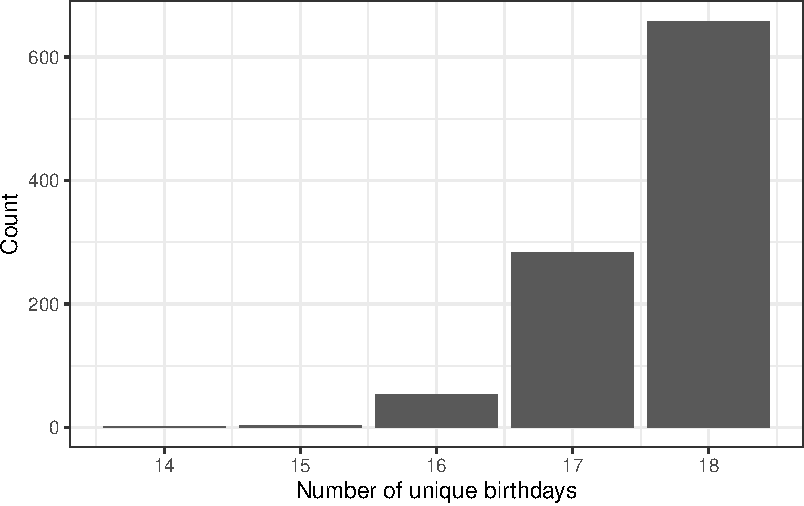
\includegraphics{07-Probability-Case-Study_files/figure-pdf/fig-bar71-1.pdf}

}

\caption{\label{fig-bar71}Bar chart of the number of unique birthdays in
the sample.}

\end{figure}%

\begin{quote}
\textbf{Exercise}:\\
What does it mean if the length of unique birthdays is 16, in terms of
matches?\footnote{It is possible that 3 people all have the same
  birthday or two sets of 2 people have the same birthday but different
  from the other pair.}
\end{quote}

\subsection{Mathematical solution}\label{mathematical-solution}

To solve this problem mathematically, we will step through the logic one
step at a time. One of the key ideas that we will see many times is the
idea of the \textbf{multiplication} rule. This idea is the foundation
for \textbf{permutation} and \textbf{combinations} which are counting
methods frequently used in probability calculations.

The first step that we take is to understand the idea of 2 or more
people with the same birthday. With 18 people, there are a great deal of
possibilities for 2 or more birthdays. We could have exactly 2 people
with the same birthday. We could have 18 people with the same birthday,
We could have 3 people with the same birthday and another 2 people with
the same birthday but different from the other 3. Accounting for all
these possibilities is too large a counting process. Instead, we will
take the approach of finding the probability of no one having a matching
birthday. Then the probability of at least 2 people having a matching
birthday is 1 minus the probability that no one has a matching birthday.
This is known as a \textbf{complementary} probability. A simpler example
is to think about rolling a single die. The probability of rolling a 6
is equivalent to 1 minus the probability of not rolling a 6.

We first need to think about all the different ways we could get 18
birthdays. This is going to be our denominator in the probability
calculation. First let's just look at 2 people. The first person could
have 365 different days for their birthday. The second person could also
have 365 different birthdays. So for each birthday of the first person
there could be 365 birthdays for the second. Thus for 2 people there are
\(365^2\) possible sets of birthdays. This is an example of the
\emph{multiplication rule}. For 18 people there are \(365^{18}\) sets of
birthdays. That is a large number. Again, this will be our denominator
in calculating the probability.

The numerator is the number of sets of birthdays with no matches. Again,
let's consider 2 people. The first person can have a birthday on any day
of the year, so 365 possibilities. Since we don't want a match, the
second person can only have 364 possibilities for a birthday. Thus we
have \(365 \times 364\) possibilities for two people to have different
birthdays.

\begin{quote}
Exercise:\\
What is the number of possibilities for 18 people so that no one has the
same birthday.
\end{quote}

The answer for 18 people is
\(365 \times 364 \times 363 ... \times 349 \times 348\). This looks like
a truncated factorial. Remember a factorial, written as \(n!\) with an
explanation point, is the product of successive positive integers. As an
example \(3!\) is \(3 \times 2 \times 1\) or 6. We could write the
multiplication for the numerator as \[\frac{365!}{(365-n)!}\] As we will
learn, the multiplication rule for the numerator is known as a
\textbf{permutation}.

We are ready to put it all together. For 18 people, the probability of 2
or more people with the same birthday is 1 minus the probability that no
one has the same birthday, which is

\[1 - \frac{\frac{365!}{(365-18)!}}{365^{18}}\] or

\[1 - \frac{\frac{365!}{347!}}{365^{18}}\]

In \texttt{R} there is a function called \texttt{factorial()} but
factorials get large fast and we will \textbf{overflow} the memory. Try
\texttt{factorial(365)} in \texttt{R} to see what happens.

\begin{Shaded}
\begin{Highlighting}[]
\FunctionTok{factorial}\NormalTok{(}\DecValTok{365}\NormalTok{)}
\end{Highlighting}
\end{Shaded}

\begin{verbatim}
[1] Inf
\end{verbatim}

It is returning \emph{infinity} because the number is too large for the
buffer. As is often the case we will have when using a computational
method, we must be clever about our approach. Instead of using
factorials we can make use of \texttt{R}s ability to work on vectors. If
we provide \texttt{R} with a vector of values, the \texttt{prod()} will
perform a product of all the elements.

\begin{Shaded}
\begin{Highlighting}[]
\DecValTok{365}\SpecialCharTok{*}\DecValTok{364}
\end{Highlighting}
\end{Shaded}

\begin{verbatim}
[1] 132860
\end{verbatim}

\begin{Shaded}
\begin{Highlighting}[]
\FunctionTok{prod}\NormalTok{(}\DecValTok{365}\SpecialCharTok{:}\DecValTok{364}\NormalTok{)}
\end{Highlighting}
\end{Shaded}

\begin{verbatim}
[1] 132860
\end{verbatim}

\begin{Shaded}
\begin{Highlighting}[]
\DecValTok{1}\SpecialCharTok{{-}} \FunctionTok{prod}\NormalTok{(}\DecValTok{365}\SpecialCharTok{:}\DecValTok{348}\NormalTok{)}\SpecialCharTok{/}\NormalTok{(}\DecValTok{365}\SpecialCharTok{\^{}}\DecValTok{18}\NormalTok{)}
\end{Highlighting}
\end{Shaded}

\begin{verbatim}
[1] 0.3469114
\end{verbatim}

\subsection{General solution}\label{general-solution}

We now have the mathematics to understand the problem. We can easily
generalize this to any number of people. To do this, we have to write a
function in \texttt{R}. As with everything in \texttt{R}, we save a
function as an object. The general format for creating a function is

\begin{Shaded}
\begin{Highlighting}[]
\NormalTok{my\_function }\OtherTok{\textless{}{-}} \ControlFlowTok{function}\NormalTok{(parameters)\{}
\NormalTok{  code }\ControlFlowTok{for} \ControlFlowTok{function}
\NormalTok{\}}
\end{Highlighting}
\end{Shaded}

For this problem we will call the function \texttt{birthday\_prob()}.
The only parameter we need is the number of people in the room,
\texttt{n}. Let's write this function.

\begin{Shaded}
\begin{Highlighting}[]
\NormalTok{birthday\_prob }\OtherTok{\textless{}{-}} \ControlFlowTok{function}\NormalTok{(}\AttributeTok{n=}\DecValTok{20}\NormalTok{)\{}
  \DecValTok{1}\SpecialCharTok{{-}} \FunctionTok{prod}\NormalTok{(}\DecValTok{365}\SpecialCharTok{:}\NormalTok{(}\DecValTok{365}\SpecialCharTok{{-}}\NormalTok{(n}\DecValTok{{-}1}\NormalTok{)))}\SpecialCharTok{/}\NormalTok{(}\DecValTok{365}\SpecialCharTok{\^{}}\NormalTok{n)}
\NormalTok{\}}
\end{Highlighting}
\end{Shaded}

Notice we assigned the function to the name \texttt{birthday\_prob}, we
told \texttt{R} to expect one argument to the function, which we are
calling \texttt{n}, and then we provide \texttt{R} with the code to find
the probability. We set a default value for \texttt{n} in case one is
not provided to prevent an error when the function is run. We will learn
more about writing functions throughout this book and in the follow-on
USAFA course, Math 378: Applied Statistical Modeling.

Test the code with a know answer.

\begin{Shaded}
\begin{Highlighting}[]
\FunctionTok{birthday\_prob}\NormalTok{(}\DecValTok{18}\NormalTok{)}
\end{Highlighting}
\end{Shaded}

\begin{verbatim}
[1] 0.3469114
\end{verbatim}

Now we can determine the probability for any size room. You may have
heard that it only takes about 23 people in a room to have a 50\%
probability of at least 2 people matching birthdays.

\begin{Shaded}
\begin{Highlighting}[]
\FunctionTok{birthday\_prob}\NormalTok{(}\DecValTok{23}\NormalTok{)}
\end{Highlighting}
\end{Shaded}

\begin{verbatim}
[1] 0.5072972
\end{verbatim}

Let's create a plot of the probability versus number of people in the
room. To do this, we need to apply the function to a vector of values.
The function \texttt{sapply()} will work or we can also use
\texttt{Vectorize()} to alter our existing function. We choose the
latter option.

First notice what happens if we input a vector into our function.

\begin{Shaded}
\begin{Highlighting}[]
\FunctionTok{birthday\_prob}\NormalTok{(}\DecValTok{1}\SpecialCharTok{:}\DecValTok{20}\NormalTok{)}
\end{Highlighting}
\end{Shaded}

\begin{verbatim}
Warning in 365:(365 - (n - 1)): numerical expression has 20 elements: only the
first used
\end{verbatim}

\begin{verbatim}
 [1] 0.0000000 0.9972603 0.9999925 1.0000000 1.0000000 1.0000000 1.0000000
 [8] 1.0000000 1.0000000 1.0000000 1.0000000 1.0000000 1.0000000 1.0000000
[15] 1.0000000 1.0000000 1.0000000 1.0000000 1.0000000 1.0000000
\end{verbatim}

It only uses the first value. There are several ways to solve this
problem. We can use the \texttt{map()} function in the \textbf{purrr}
package. This idea of mapping a function to a vector is important in
data science. It is used in scenarios where there is a lot of data. In
this case the idea of map-reduce is used to make the analysis amenable
to parallel computing.

\begin{Shaded}
\begin{Highlighting}[]
\FunctionTok{map\_dbl}\NormalTok{(}\DecValTok{1}\SpecialCharTok{:}\DecValTok{20}\NormalTok{,birthday\_prob)}
\end{Highlighting}
\end{Shaded}

\begin{verbatim}
 [1] 0.000000000 0.002739726 0.008204166 0.016355912 0.027135574 0.040462484
 [7] 0.056235703 0.074335292 0.094623834 0.116948178 0.141141378 0.167024789
[13] 0.194410275 0.223102512 0.252901320 0.283604005 0.315007665 0.346911418
[19] 0.379118526 0.411438384
\end{verbatim}

We could also just vectorize the function.

\begin{Shaded}
\begin{Highlighting}[]
\NormalTok{birthday\_prob }\OtherTok{\textless{}{-}} \FunctionTok{Vectorize}\NormalTok{(birthday\_prob)}
\end{Highlighting}
\end{Shaded}

Now notice what happens.

\begin{Shaded}
\begin{Highlighting}[]
\FunctionTok{birthday\_prob}\NormalTok{(}\DecValTok{1}\SpecialCharTok{:}\DecValTok{20}\NormalTok{)}
\end{Highlighting}
\end{Shaded}

\begin{verbatim}
 [1] 0.000000000 0.002739726 0.008204166 0.016355912 0.027135574 0.040462484
 [7] 0.056235703 0.074335292 0.094623834 0.116948178 0.141141378 0.167024789
[13] 0.194410275 0.223102512 0.252901320 0.283604005 0.315007665 0.346911418
[19] 0.379118526 0.411438384
\end{verbatim}

We are good to go. Let's create our line plot, Figure~\ref{fig-line71}.

\begin{Shaded}
\begin{Highlighting}[]
\FunctionTok{gf\_line}\NormalTok{(}\FunctionTok{birthday\_prob}\NormalTok{(}\DecValTok{1}\SpecialCharTok{:}\DecValTok{100}\NormalTok{)}\SpecialCharTok{\textasciitilde{}} \FunctionTok{seq}\NormalTok{(}\DecValTok{1}\NormalTok{,}\DecValTok{100}\NormalTok{),}
        \AttributeTok{xlab=}\StringTok{"Number of People"}\NormalTok{,}
        \AttributeTok{ylab=}\StringTok{"Probability of Match"}\NormalTok{,}
        \AttributeTok{title=}\StringTok{"Probability of at least 2 people with matching birthdays"}\NormalTok{) }\SpecialCharTok{\%\textgreater{}\%}
  \FunctionTok{gf\_theme}\NormalTok{(}\FunctionTok{theme\_bw}\NormalTok{())}
\end{Highlighting}
\end{Shaded}

\begin{figure}[H]

\centering{

\includegraphics{07-Probability-Case-Study_files/figure-pdf/fig-line71-1.pdf}

}

\caption{\label{fig-line71}The probability of at least 2 people having
mathcing birthdays.}

\end{figure}%

Is this what you expected the curve to look like? We, the authors, did
not expect this. It has a sigmodial shape with a large increase in the
middle range and flatten in the tails.

\subsection{Data science approach}\label{data-science-approach}

The final approach we will take is one based on data, a data science
approach. In the \textbf{mosaicData} package is a data set called
\texttt{Births} that contains the number of births in the US from 1969
to 1988. This data will allow us to estimate the number of births on any
day of the year. This allows us to eliminate the reliance on the
assumption that each day is equally likely. Let's first
\texttt{inspect()} the data object.

\begin{Shaded}
\begin{Highlighting}[]
\FunctionTok{inspect}\NormalTok{(Births)}
\end{Highlighting}
\end{Shaded}

\begin{verbatim}

categorical variables:  
  name   class levels    n missing
1 wday ordered      7 7305       0
                                   distribution
1 Wed (14.3%), Thu (14.3%), Fri (14.3%) ...    

Date variables:  
  name class      first       last min_diff max_diff    n missing
1 date  Date 1969-01-01 1988-12-31   1 days   1 days 7305       0

quantitative variables:  
          name   class  min   Q1 median    Q3   max        mean          sd
1       births integer 6675 8792   9622 10510 12851 9648.940178 1127.315229
2         year integer 1969 1974   1979  1984  1988 1978.501027    5.766735
3        month integer    1    4      7    10    12    6.522930    3.448939
4  day_of_year integer    1   93    184   275   366  183.753593  105.621885
5 day_of_month integer    1    8     16    23    31   15.729637    8.800694
6  day_of_week integer    1    2      4     6     7    4.000274    1.999795
     n missing
1 7305       0
2 7305       0
3 7305       0
4 7305       0
5 7305       0
6 7305       0
\end{verbatim}

It could be argued that we could randomly pick one year and use it.
Let's see what happens if we just used 1969. Figure~\ref{fig-scat71} is
a scatter plot of the number of births in 1969 for each day of the year.

\begin{Shaded}
\begin{Highlighting}[]
\NormalTok{Births }\SpecialCharTok{\%\textgreater{}\%}
  \FunctionTok{filter}\NormalTok{(year }\SpecialCharTok{==} \DecValTok{1969}\NormalTok{) }\SpecialCharTok{\%\textgreater{}\%}
  \FunctionTok{gf\_point}\NormalTok{(births}\SpecialCharTok{\textasciitilde{}}\NormalTok{day\_of\_year) }\SpecialCharTok{\%\textgreater{}\%}
  \FunctionTok{gf\_theme}\NormalTok{(}\FunctionTok{theme\_bw}\NormalTok{()) }\SpecialCharTok{\%\textgreater{}\%}
  \FunctionTok{gf\_labs}\NormalTok{(}\AttributeTok{x=}\StringTok{"Day of the Year"}\NormalTok{,}\AttributeTok{y=}\StringTok{"Number of Births"}\NormalTok{)}
\end{Highlighting}
\end{Shaded}

\begin{figure}[H]

\centering{

\includegraphics{07-Probability-Case-Study_files/figure-pdf/fig-scat71-1.pdf}

}

\caption{\label{fig-scat71}The number of births for each day of the year
in 1969.}

\end{figure}%

\begin{quote}
\textbf{Exercise}:\\
What patterns do you see in Figure~\ref{fig-scat71}? What might explain
them?
\end{quote}

There are definitely bands appearing in the data which could be the day
of the week; there are less birthdays on the weekend. There is also
seasonality with more birthdays in the summer and fall. There is also
probably an impact from holidays.

Quickly, let's look at the impact of day of the week by using color for
day of the week. Figure~\ref{fig-scat72} makes it clear that the
weekends have less number of births as compared to the work week.

\begin{Shaded}
\begin{Highlighting}[]
\NormalTok{Births }\SpecialCharTok{\%\textgreater{}\%}
  \FunctionTok{filter}\NormalTok{(year }\SpecialCharTok{==} \DecValTok{1969}\NormalTok{) }\SpecialCharTok{\%\textgreater{}\%}
  \FunctionTok{gf\_point}\NormalTok{(births}\SpecialCharTok{\textasciitilde{}}\NormalTok{day\_of\_year,}\AttributeTok{color=}\SpecialCharTok{\textasciitilde{}}\FunctionTok{factor}\NormalTok{(day\_of\_week)) }\SpecialCharTok{\%\textgreater{}\%}
  \FunctionTok{gf\_labs}\NormalTok{(}\AttributeTok{x=}\StringTok{"Day of the Year"}\NormalTok{,}\AttributeTok{col=}\StringTok{"Day of Week"}\NormalTok{) }\SpecialCharTok{\%\textgreater{}\%}
  \FunctionTok{gf\_theme}\NormalTok{(}\FunctionTok{theme\_bw}\NormalTok{())}
\end{Highlighting}
\end{Shaded}

\begin{figure}[H]

\centering{

\includegraphics{07-Probability-Case-Study_files/figure-pdf/fig-scat72-1.pdf}

}

\caption{\label{fig-scat72}The number of births for each day of the year
in 1969 broken down by day of the week.}

\end{figure}%

By only using one year, this data might give poor results since holidays
will fall on certain days of the week and the weekends will also be
impacted. Note that we also still have the problem of leap years.

\begin{Shaded}
\begin{Highlighting}[]
\NormalTok{Births }\SpecialCharTok{\%\textgreater{}\%}
  \FunctionTok{group\_by}\NormalTok{(year) }\SpecialCharTok{\%\textgreater{}\%}
  \FunctionTok{summarise}\NormalTok{(}\AttributeTok{n=}\FunctionTok{n}\NormalTok{())}
\end{Highlighting}
\end{Shaded}

\begin{verbatim}
# A tibble: 20 x 2
    year     n
   <int> <int>
 1  1969   365
 2  1970   365
 3  1971   365
 4  1972   366
 5  1973   365
 6  1974   365
 7  1975   365
 8  1976   366
 9  1977   365
10  1978   365
11  1979   365
12  1980   366
13  1981   365
14  1982   365
15  1983   365
16  1984   366
17  1985   365
18  1986   365
19  1987   365
20  1988   366
\end{verbatim}

The years 1972, 1976, 1980, 1984, and 1988 are all leap years. At this
point, to make the analysis easier, we will drop those years.

\begin{Shaded}
\begin{Highlighting}[]
\NormalTok{Births }\SpecialCharTok{\%\textgreater{}\%}
  \FunctionTok{filter}\NormalTok{(}\SpecialCharTok{!}\NormalTok{(year }\SpecialCharTok{\%in\%} \FunctionTok{c}\NormalTok{(}\DecValTok{1972}\NormalTok{,}\DecValTok{1976}\NormalTok{,}\DecValTok{1980}\NormalTok{,}\DecValTok{1984}\NormalTok{,}\DecValTok{1988}\NormalTok{))) }\SpecialCharTok{\%\textgreater{}\%}
  \FunctionTok{group\_by}\NormalTok{(year) }\SpecialCharTok{\%\textgreater{}\%}
  \FunctionTok{summarise}\NormalTok{(}\AttributeTok{n=}\FunctionTok{n}\NormalTok{())}
\end{Highlighting}
\end{Shaded}

\begin{verbatim}
# A tibble: 15 x 2
    year     n
   <int> <int>
 1  1969   365
 2  1970   365
 3  1971   365
 4  1973   365
 5  1974   365
 6  1975   365
 7  1977   365
 8  1978   365
 9  1979   365
10  1981   365
11  1982   365
12  1983   365
13  1985   365
14  1986   365
15  1987   365
\end{verbatim}

Notice in \texttt{filter()} we used the \texttt{\%in\%} argument. This
is a \textbf{logical} argument checking if \texttt{year} is one of the
values. The \texttt{!} at the front negates this in a sense requiring
\texttt{year} not to be one of those values.`

We are almost ready to simulate. We need to get the count of
\texttt{births} on each day of the year for the non-leap years.

\begin{Shaded}
\begin{Highlighting}[]
\NormalTok{birth\_data }\OtherTok{\textless{}{-}}\NormalTok{ Births }\SpecialCharTok{\%\textgreater{}\%}
  \FunctionTok{filter}\NormalTok{(}\SpecialCharTok{!}\NormalTok{(year }\SpecialCharTok{\%in\%} \FunctionTok{c}\NormalTok{(}\DecValTok{1972}\NormalTok{,}\DecValTok{1976}\NormalTok{,}\DecValTok{1980}\NormalTok{,}\DecValTok{1984}\NormalTok{,}\DecValTok{1988}\NormalTok{))) }\SpecialCharTok{\%\textgreater{}\%}
  \FunctionTok{group\_by}\NormalTok{(day\_of\_year) }\SpecialCharTok{\%\textgreater{}\%}
  \FunctionTok{summarise}\NormalTok{(}\AttributeTok{n=}\FunctionTok{sum}\NormalTok{(births)) }
\end{Highlighting}
\end{Shaded}

\begin{Shaded}
\begin{Highlighting}[]
\FunctionTok{head}\NormalTok{(birth\_data)}
\end{Highlighting}
\end{Shaded}

\begin{verbatim}
# A tibble: 6 x 2
  day_of_year      n
        <int>  <int>
1           1 120635
2           2 129042
3           3 135901
4           4 136298
5           5 137319
6           6 140044
\end{verbatim}

Let's look at a plot of the number of births versus day of the year. We
combined years in Figure~\ref{fig-scat73}.

\begin{Shaded}
\begin{Highlighting}[]
\NormalTok{birth\_data }\SpecialCharTok{\%\textgreater{}\%}
  \FunctionTok{gf\_point}\NormalTok{(n}\SpecialCharTok{\textasciitilde{}}\NormalTok{day\_of\_year,}
          \AttributeTok{xlab=}\StringTok{"Day of the year"}\NormalTok{,}
          \AttributeTok{ylab=}\StringTok{"Number of births"}\NormalTok{) }\SpecialCharTok{\%\textgreater{}\%}
  \FunctionTok{gf\_theme}\NormalTok{(}\FunctionTok{theme\_bw}\NormalTok{())}
\end{Highlighting}
\end{Shaded}

\begin{figure}[H]

\centering{

\includegraphics{07-Probability-Case-Study_files/figure-pdf/fig-scat73-1.pdf}

}

\caption{\label{fig-scat73}Number of births by day of the year for all
years.}

\end{figure}%

This curve has the seasonal cycling we would expect. The smaller scale
cycling is unexpected. Maybe because we are dropping the leap years, we
are getting some days appearing in our time interval more frequently on
weekends. We leave it to you to investigate this phenomenon.

We use these counts as weights in a sampling process. Days with more
births will have a higher probability of being selected. Days such as
Christmas and Christmas Eve have a lower probability of being selected.
Let's save the weights in an object to use in the \texttt{sample()}
function.

\begin{Shaded}
\begin{Highlighting}[]
\NormalTok{birth\_data\_weights }\OtherTok{\textless{}{-}}\NormalTok{ birth\_data }\SpecialCharTok{\%\textgreater{}\%}
  \FunctionTok{select}\NormalTok{(n) }\SpecialCharTok{\%\textgreater{}\%}
  \FunctionTok{pull}\NormalTok{()}
\end{Highlighting}
\end{Shaded}

The \texttt{pull()} function pulls the vectors of values out of the data
frame format into a vector format which the \texttt{sample()} needs.

Now let's simulate the problem. The probability of a match should change
slightly, maybe go down slightly?, but not much since most of the days
have about the same probability or number of occurrences.

\begin{Shaded}
\begin{Highlighting}[]
\FunctionTok{set.seed}\NormalTok{(}\DecValTok{20}\NormalTok{)}
\NormalTok{(}\FunctionTok{do}\NormalTok{(}\DecValTok{1000}\NormalTok{)}\SpecialCharTok{*}\FunctionTok{length}\NormalTok{(}\FunctionTok{unique}\NormalTok{(}\FunctionTok{sample}\NormalTok{(days,}\AttributeTok{size=}\DecValTok{18}\NormalTok{,}\AttributeTok{replace =} \ConstantTok{TRUE}\NormalTok{,}\AttributeTok{prob=}\NormalTok{birth\_data\_weights)))) }\SpecialCharTok{\%\textgreater{}\%}
  \FunctionTok{mutate}\NormalTok{(}\AttributeTok{match=}\FunctionTok{if\_else}\NormalTok{(length}\SpecialCharTok{==}\DecValTok{18}\NormalTok{,}\DecValTok{0}\NormalTok{,}\DecValTok{1}\NormalTok{)) }\SpecialCharTok{\%\textgreater{}\%}
  \FunctionTok{summarise}\NormalTok{(}\AttributeTok{prob=}\FunctionTok{mean}\NormalTok{(match))}
\end{Highlighting}
\end{Shaded}

\begin{verbatim}
   prob
1 0.352
\end{verbatim}

We could not solve this problem of varying frequency of birth days using
mathematics, at least as far as we know.

Cool stuff, let's get to learning more about probability models in the
next chapters.

\section{Homework Problems}\label{homework-problems-6}

\begin{enumerate}
\def\labelenumi{\arabic{enumi}.}
\tightlist
\item
  \textbf{Exactly 2 people with the same birthday - Simulation}.
  Complete a similar analysis for case where exactly 2 people in a room
  of 23 people have the same birthday. In this exercise you will use a
  computational simulation.
\end{enumerate}

\begin{enumerate}
\def\labelenumi{\alph{enumi}.}
\tightlist
\item
  Create a new R Markdown file and create a report. Yes, we know you
  could use this file but we want you to practice generating your own
  report.\\
\item
  Simulate having 23 people in the class with each day of the year
  equally likely. Find the cases where exactly 2 people have the same
  birthday, you will have to alter the code from the Notes more than
  changing 18 to 23.\\
\item
  Plot the frequency of occurrences as a bar chart.\\
\item
  Estimate the probability of exactly two people having the same
  birthday.
\end{enumerate}

\begin{enumerate}
\def\labelenumi{\arabic{enumi}.}
\setcounter{enumi}{1}
\tightlist
\item
  \textbf{Exactly 2 people with the same birthday - Mathematical}.
  Repeat problem 1 but do it mathematically. As a big hint, you will
  need to use the \texttt{choose()} function. The idea is that with 23
  people we need to choose 2 of them to match. We thus need to multiply,
  the multiplication rule again, by \texttt{choose(23,2)}. If you are
  having trouble, work with a total of 3 people in the room first.
\end{enumerate}

\begin{enumerate}
\def\labelenumi{\alph{enumi}.}
\tightlist
\item
  Find a formula to determine the exact probability of exactly 2 people
  in a room of 23 having the same birthday.\\
\item
  Generalize your solution to any number \texttt{n} people in the room
  and create a function.\\
\item
  Vectorize the function.\\
\item
  Plot the probability of exactly 2 people having the same birthday
  versus number of people in the room.\\
\item
  Comment on the shape of the curve and explain it.
\end{enumerate}

\section*{\texorpdfstring{\href{https://ds-usafa.github.io/CPS-Solutions-Manual/CS2.html}{Solutions
Manual}}{Solutions Manual}}\label{solutions-manual-7}
\addcontentsline{toc}{section}{\href{https://ds-usafa.github.io/CPS-Solutions-Manual/CS2.html}{Solutions
Manual}}

\markright{Solutions Manual}

\chapter{Probability Basics}\label{PROBRULES}

\newcommand{\E}{\mbox{E}}
\newcommand{\Var}{\mbox{Var}}
\newcommand{\Cov}{\mbox{Cov}}
\newcommand{\Prob}{\mbox{P}}
\newcommand*\diff{\mathop{}\!\mathrm{d}}

\section{Objectives}\label{objectives-8}

\begin{enumerate}
\def\labelenumi{\arabic{enumi})}
\item
  Define and use properly in context all new terminology related to
  probability, including: \emph{sample space}, \emph{outcome},
  \emph{event}, \emph{subset}, \emph{intersection}, \emph{union},
  \emph{complement}, \emph{probability}, \emph{mutually exclusive},
  \emph{exhaustive}, \emph{independent}, \emph{multiplication rule},
  \emph{permutation}, \emph{combination}.
\item
  Apply basic probability and counting rules to find probabilities.
\item
  Describe the basic axioms of probability.
\item
  Use \texttt{R} to calculate and simulate probabilities of events.
\end{enumerate}

\section{Probability vs Statistics}\label{probability-vs-statistics}

As a review, remember this book is divided into four general blocks:
data collection/summary, probability models, inference and statistical
modeling/prediction. This second block, probability, is the study of
stochastic (random) processes and their properties. Specifically, we
will explore random experiments. As its name suggests, a random
experiment is an experiment whose outcome is not predictable with exact
certainty. In the statistical models we develop in the last two blocks
of this book, we will use other variables to explain the variance of the
outcome of interest. Any remaining variance is modeled with probability
models.

Even though an outcome is determined by chance, this does not mean that
we know nothing about the random experiment. Our favorite simple example
is that of a coin flip. If we flip a coin, the possible outcomes are
heads and tails. We don't know for sure what outcome will occur, but
this doesn't mean we don't know anything about the experiment. If we
assume the coin is fair, we know that each outcome is equally likely.
Also, we know that if we flip the coin 100 times (independently), we are
likely, the highest frequency event, to see around 50 heads, and very
unlikely to see 10 heads or fewer.

It is important to distinguish probability from inference and modeling.
In probability, we consider a known random experiment, including knowing
the parameters, and answer questions about what we expect to see from
this random experiment. In statistics (inference and modeling), we
consider data (the results of a mysterious random experiment) and infer
about the underlying process. For example, suppose we have a coin and we
are unsure whether this coin is fair or unfair, the parameter is
unknown. We flipped it 20 times and it landed on heads 14 times.
Inferential statistics will help us answer questions about the
underlying process (could this coin be unfair?).

\begin{figure}[H]

{\centering \includegraphics{figures/Prob_Stats.png}

}

\caption{A graphical representation of probability and statistics. In
probability, we describe what we expect to happen if we know that
underlying process; in statistics, we don't know the underlying process,
and must infer based on representative samples.}

\end{figure}%

This block (10 chapters or so) is devoted to the study of random
experiments. First, we will explore simple experiments, counting rule
problems, and conditional probability. Next, we will introduce the
concept of a random variable and the properties of random variables.
Following this, we will cover common distributions of discrete and
continuous random variables. We will end the block on multivariate
probability (joint distributions and covariance).

\section{Basic probability terms}\label{basic-probability-terms}

We will start our work with some definitions and examples.

\subsection{Sample space}\label{sample-space}

Suppose we have a random experiment. The \emph{sample space} of this
experiment, \(S\), is the set of all possible results of that
experiment. For example, in the case of a coin flip, we could write
\(S=\{H,T\}\). Each element of the sample space is considered an
\emph{outcome}. An \emph{event} is a set of outcomes, it is a subset of
the sample space.

\begin{quote}
\emph{Example}:\\
Let's let \texttt{R} flip a coin for us and record the number of heads
and tails. We will have \texttt{R} flip the coin twice. What is the
sample space, what is an example of an outcome, and what is an example
of an event.
\end{quote}

We will load the \textbf{mosaic} package as it has a function
\texttt{rflip()} that will simulate flipping a coin.

\begin{Shaded}
\begin{Highlighting}[]
\FunctionTok{library}\NormalTok{(mosaic)}
\end{Highlighting}
\end{Shaded}

\begin{Shaded}
\begin{Highlighting}[]
\FunctionTok{set.seed}\NormalTok{(}\DecValTok{18}\NormalTok{)}
\FunctionTok{rflip}\NormalTok{(}\DecValTok{2}\NormalTok{)}
\end{Highlighting}
\end{Shaded}

\begin{verbatim}

Flipping 2 coins [ Prob(Heads) = 0.5 ] ...

H H

Number of Heads: 2 [Proportion Heads: 1]
\end{verbatim}

The sample space is \(S=\{HH, TH, HT, TT\}\), an example of an outcome
is \(HH\) which we see in the output from \texttt{R}, and finally an
example of an event is the number of heads, which in this case takes on
the values 0, 1, and 2. Another example of an event is ``At least one
heads''. In this case the event would be \(\{HH,TH, HT\}\). Also notice
that \(TH\) is different from \(HT\) as an outcome; this is because
those are different outcomes from flipping a coin twice.

\begin{quote}
\emph{Example of Event}:\\
Suppose you arrive at a rental car counter and they show you a list of
available vehicles, and one is picked for you at random. The sample
space in this experiment is \[
S=\{\mbox{red sedan}, \mbox{blue sedan}, \mbox{red truck}, \mbox{grey truck}, \mbox{grey SUV}, \mbox{black SUV}, \mbox{blue SUV}\}.
\]
\end{quote}

Each vehicle represents a possible outcome of the experiment. Let \(A\)
be the event that a blue vehicle is selected. This event contains the
outcomes \texttt{blue\ sedan} and \texttt{blue\ SUV}.

\subsection{Union and intersection}\label{union-and-intersection}

Suppose we have two events \(A\) and \(B\).

\begin{enumerate}
\def\labelenumi{\arabic{enumi})}
\item
  \(A\) is considered a \emph{subset} of \(B\) if all of the outcomes of
  \(A\) are also contained in \(B\). This is denoted as \(A \subset B\).
\item
  The \emph{intersection} of \(A\) and \(B\) is all of the outcomes
  contained in both \(A\) and \(B\). This is denoted as \(A \cap B\).
\item
  The \emph{union} of \(A\) and \(B\) is all of the outcomes contained
  in either \(A\) or \(B\), or both. This is denoted as \(A \cup B\).
\item
  The \emph{complement} of \(A\) is all of the outcomes not contained in
  \(A\). This is denoted as \(A^C\) or \(A'\).
\end{enumerate}

Note: Here we are treating events as sets and the above definitions are
basic set operations.

It is sometimes helpful when reading probability notation to think of
Union as an \emph{or} and Intersection as an \emph{and}.

\begin{quote}
\emph{Example}:\\
Consider our rental car example above. Let \(A\) be the event that a
blue vehicle is selected, let \(B\) be the event that a black vehicle is
selected, and let \(C\) be the event that an SUV is selected.
\end{quote}

First, let's list all of the outcomes of each event.
\(A = \{\mbox{blue sedan},\mbox{blue SUV}\}\),
\(B=\{\mbox{black SUV}\}\), and
\(C= \{\mbox{grey SUV}, \mbox{black SUV}, \mbox{blue SUV}\}\).

Since all outcomes in \(B\) are contained in \(C\), we know that \(B\)
is a subset of \(C\), or \(B\subset C\). Also, since \(A\) and \(B\)
have no outcomes in common, \(A \cap B = \emptyset\). Note that
\(\emptyset = \{ \}\) is the empty set and contains no elements.
Further,
\(A \cup C = \{\mbox{blue sedan}, \mbox{grey SUV}, \mbox{black SUV}, \mbox{blue SUV}\}\).

\section{Probability}\label{probability}

\emph{Probability} is a number assigned to an event or outcome that
describes how likely it is to occur. A probability model assigns a
probability to each element of the sample space. What makes a
probability model is not just the values assigned to each element but
the idea this model contains all the information about the outcomes and
there are no other explanatory variables involved.

A probability model can be thought of as a function that maps outcomes,
or events, to a real number in the interval \([0,1]\).

There are some basic axioms of probability you should know, although
this list is not complete. Let \(S\) be the sample space of a random
experiment and let \(A\) be an event where \(A\subset S\).

\begin{enumerate}
\def\labelenumi{\arabic{enumi})}
\item
  \(\mbox{P}(A) \geq 0\).
\item
  \(\mbox{P}(S) = 1\).
\end{enumerate}

These two axioms essentially say that probability must be positive, and
the probability of all outcomes must sum to 1.

\subsection{Probability properties}\label{probability-properties}

Let \(A\) and \(B\) be events in a random experiment. Most of these can
be proven fairly easily.

\begin{enumerate}
\def\labelenumi{\arabic{enumi})}
\item
  \(\mbox{P}(\emptyset)=0\)
\item
  \(\mbox{P}(A')=1-\mbox{P}(A)\) We used this in the case study.
\item
  If \(A\subset B\), then \(\mbox{P}(A)\leq \mbox{P}(B)\).
\item
  \(\mbox{P}(A\cup B) = \mbox{P}(A)+\mbox{P}(B)-\mbox{P}(A\cap B)\).
  This property can be generalized to more than two events. The
  intersection is subtracted because outcomes in both events \(A\) and
  \(B\) get counted twice in the first sum.
\item
  Law of Total Probability: Let \(B_1, B_2,...,B_n\) be \textbf{mutually
  exclusive}, this means disjoint or no outcomes in common, and
  \textbf{exhaustive}, this means the union of all the events labeled
  with a \(B\) is the sample space. Then
\end{enumerate}

\[
\mbox{P}(A)=\mbox{P}(A\cap B_1)+\mbox{P}(A\cap B_2)+...+\mbox{P}(A\cap B_n)
\]

A specific application of this law appears in Bayes' Rule (more to
follow). It says that
\(\mbox{P}(A)=\mbox{P}(A \cap B)+\mbox{P}(A \cap B')\). Essentially, it
points out that \(A\) can be partitioned into two parts: 1) everything
in \(A\) and \(B\) and 2) everything in \(A\) and not in \(B\).

\begin{quote}
\emph{Example}:\\
Consider rolling a six sided die. Let event \(A\) be the number showing
is less than 5. Let event \(B\) be the number is even. Then
\end{quote}

\[\mbox{P}(A)=\mbox{P}(A \cap B) + \mbox{P}(A \cap B')\]

\[
\mbox{P}(< 5)=\mbox{P}(<5 \cap Even)+\mbox{P}(<5 \cap Odd)
\]

\begin{enumerate}
\def\labelenumi{\arabic{enumi})}
\setcounter{enumi}{5}
\tightlist
\item
  DeMorgan's Laws: \[
  \mbox{P}((A \cup B)')=\mbox{P}(A' \cap B')
  \] \[
  \mbox{P}((A \cap B)')=\mbox{P}(A' \cup B')
  \]
\end{enumerate}

\subsection{Equally likely scenarios}\label{equally-likely-scenarios}

In some random experiments, outcomes can be defined such that each
individual outcome is equally likely. In this case, probability becomes
a counting problem. Let \(A\) be an event in an experiment where each
outcome is equally likely. \[
\mbox{P}(A)=\frac{\mbox{# of outcomes in A}}{\mbox{# of outcomes in S}}
\]

\begin{quote}
\emph{Example}:\\
Suppose a family has three children, with each child being either a boy
(B) or girl (G). Assume that the likelihood of boys and girls are equal
and \textbf{independent}, this is the idea that the probability of the
gender of the second child does not change based on the gender of the
first child. The sample space can be written as: \[
S=\{\mbox{BBB},\mbox{BBG},\mbox{BGB},\mbox{BGG},\mbox{GBB},\mbox{GBG},\mbox{GGB},\mbox{GGG}\}
\] What is the probability that the family has exactly 2 girls?
\end{quote}

This only happens in three ways: BGG, GBG, and GGB. Thus, the
probability of exactly 2 girls is 3/8 or 0.375.

\section{Counting rules}\label{counting-rules}

There are three types of counting problems we will consider. In each
case, the multiplication rule is being used and all that changes is
whether an element is allowed to be reused, replacement, and whether the
order of selection matters. This latter question is difficult. Each case
will be demonstrated with an example.

\subsection{Multiplication rule 1: Order matters, sample with
replacement}\label{multiplication-rule-1-order-matters-sample-with-replacement}

The multiplication rule is at the center of each of the three methods.
In this first case we are using the idea that order matters and items
can be reused. Let's use an example to help.

\begin{quote}
\emph{Example}:\\
A license plate consists of three numeric digits (0-9) followed by three
single letters (A-Z). How many possible license plates exist?
\end{quote}

We can divide this problem into two sections. In the numeric section, we
are selecting 3 objects from 10, with replacement. This means that a
number can be used more than once. Order clearly matters because a
license plate starting with ``432'' is distinct from a license plate
starting with ``234''. There are \(10^3 = 1000\) ways to select the
first three digits; 10 for the first, 10 for the second, and 10 for the
third. Why do you multiply and not add?\footnote{Multiplication is
  repeated adding so in a sense we are adding. However in a more serious
  tone, for this problem for every first number there are 10
  possibilities for the second number and for every second number there
  are 10 possibilities for the third numbers. This is multiplication.}

In the alphabet section, we are selecting 3 objects from 26, where order
matters. Thus, there are \(26^3=17576\) ways to select the last three
letters of the plate. Combined, there are
\(10^3 \times 26^3 = 17576000\) ways to select license plates. Visually,
\[
\underbrace{\underline{\quad 10 \quad }}_\text{number} \times \underbrace{\underline{\quad 10 \quad }}_\text{number} \times \underbrace{\underline{\quad 10 \quad }}_\text{number} \times \underbrace{\underline{\quad 26 \quad }}_\text{letter} \times \underbrace{\underline{\quad 26 \quad }}_\text{letter} \times \underbrace{\underline{\quad 26 \quad }}_\text{letter} = 17,576,000
\]

Next we are going to use this new counting method to find a probability.

\begin{quote}
\emph{Exercise}:\\
What is the probability a license plate starts with the number ``8'' or
``0'' and ends with the letter ``B''?
\end{quote}

In order to find this probability, we simply need to determine the
number of ways to select a license plate starting with ``8'' or ``0''
and ending with the letter ``B''. We can visually represent this event:
\[
\underbrace{\underline{\quad 2 \quad }}_\text{8 or 0} \times \underbrace{\underline{\quad 10 \quad }}_\text{number} \times \underbrace{\underline{\quad 10 \quad }}_\text{number} \times \underbrace{\underline{\quad 26 \quad }}_\text{letter} \times \underbrace{\underline{\quad 26 \quad }}_\text{letter} \times \underbrace{\underline{\quad 1 \quad }}_\text{B} = 135,200
\]

Dividing this number by the total number of possible license plates
yields the probability of this event occurring.

\begin{Shaded}
\begin{Highlighting}[]
\NormalTok{denom}\OtherTok{\textless{}{-}}\DecValTok{10}\SpecialCharTok{*}\DecValTok{10}\SpecialCharTok{*}\DecValTok{10}\SpecialCharTok{*}\DecValTok{26}\SpecialCharTok{*}\DecValTok{26}\SpecialCharTok{*}\DecValTok{26}
\NormalTok{num}\OtherTok{\textless{}{-}}\DecValTok{2}\SpecialCharTok{*}\DecValTok{10}\SpecialCharTok{*}\DecValTok{10}\SpecialCharTok{*}\DecValTok{26}\SpecialCharTok{*}\DecValTok{26}\SpecialCharTok{*}\DecValTok{1}
\NormalTok{num}\SpecialCharTok{/}\NormalTok{denom}
\end{Highlighting}
\end{Shaded}

\begin{verbatim}
[1] 0.007692308
\end{verbatim}

The probability of obtaining a license plate starting with ``8'' or
``0'' and ending with ``B'' is 0.0077. Simulating this would be
difficult because we would need special functions to check the first
number and last letter. This gets into \textbf{text mining} an important
subject in data science but unfortunately we don't have much time in
this book for the topic.

\subsection{Multiplication rule 2 (Permutation): Order Matters, Sampling
Without
Replacement}\label{multiplication-rule-2-permutation-order-matters-sampling-without-replacement}

Consider a random experiment where we sample from a group of size \(n\),
\textbf{without} replacement, and the outcome of the experiment depends
on the order of the outcomes. The number of ways to select \(k\) objects
is given by \(n(n-1)(n-2)...(n-k+1)\). This is known as a permutation
and is sometimes written as \[
{}_nP_{k} = \frac{n!}{(n-k)!}
\]

Recall that \(n!\) is read as \(n\) factorial and represents the number
of ways to arrange \(n\) objects.

\begin{quote}
\emph{Example}:\\
Twenty-five friends participate in a Halloween costume party. Three
prizes are given during the party: most creative costume, scariest
costume, and funniest costume. No one can win more than one prize. How
many possible ways can the prizes by distributed?
\end{quote}

There are \(k=3\) prizes to be assigned to \(n=25\) people. Once someone
is selected for a prize, they are removed from the pool of eligibles. In
other words, we are sampling without replacement. Also, order matters.
For example, if Tom, Mike, and Jane, win most creative, scariest and
funniest costume, respectively, this is a different outcome than if Mike
won creative, Jane won scariest and Tom won funniest. Thus, the number
of ways the prizes can be distributed is given by
\({}_{25}P_3 = \frac{25!}{22!} = 13,800\). A more visually pleasing way
to express this would be: \[
\underbrace{\underline{\quad 25 \quad }}_\text{most creative} \times \underbrace{\underline{\quad 24 \quad }}_\text{scariest} \times \underbrace{\underline{\quad 23 \quad }}_\text{funniest} = 13,800
\]

Notice that it is sometime difficult to determine if order matters or
not in a problem, but in this example the name of the prize was a hint
that indeed order matters.

Let's use the idea of a permutation to calculate a probability.

\begin{quote}
\emph{Exercise}:\\
Assume that all 25 participants are equally likely to win any one of the
three prizes. What is the probability that Tom doesn't win any of them?
\end{quote}

Just like in the previous probability calculation, we simply need to
count the number of ways Tom doesn't win any prize. In other words, we
need to count the number of ways that prizes are distributed without
Tom. So, remove Tom from the group of 25 eligible participants. The
number of ways Tom doesn't get a prize is
\({}_{24}P_3 = \frac{24!}{21!}=12,144\). Again visually: \[
\underbrace{\underline{\quad 24 \quad }}_\text{most creative} \times \underbrace{\underline{\quad 23 \quad }}_\text{scariest} \times \underbrace{\underline{\quad 22 \quad }}_\text{funniest} = 12,144
\]

The probability Tom doesn't get a prize is simply the second number
divided by the first:

\begin{Shaded}
\begin{Highlighting}[]
\NormalTok{denom}\OtherTok{\textless{}{-}}\FunctionTok{factorial}\NormalTok{(}\DecValTok{25}\NormalTok{)}\SpecialCharTok{/}\FunctionTok{factorial}\NormalTok{(}\DecValTok{25{-}3}\NormalTok{)}
\CommentTok{\# Or, denom\textless{}{-}25*24*23}
\NormalTok{num}\OtherTok{\textless{}{-}}\DecValTok{24}\SpecialCharTok{*}\DecValTok{23}\SpecialCharTok{*}\DecValTok{22}
\NormalTok{num}\SpecialCharTok{/}\NormalTok{denom}
\end{Highlighting}
\end{Shaded}

\begin{verbatim}
[1] 0.88
\end{verbatim}

\subsection{Multiplication rule 3 (Combination): Order Does Not Matter,
Sampling Without
Replacement}\label{multiplication-rule-3-combination-order-does-not-matter-sampling-without-replacement}

Consider a random experiment where we sample from a group of size \(n\),
without replacement, and the outcome of the experiment does not depend
on the order of the outcomes. The number of ways to select \(k\) objects
is given by \(\frac{n!} {(n-k)!k!}\). This is known as a combination and
is written as: \[
\binom{n}{k} = \frac{n!}{(n-k)!k!} 
\]

This is read as ``\(n\) choose \(k\)''. Take a moment to compare
combinations to permutations, discussed in Rule 2. The difference
between these two rules is that in a combination, order no longer
matters. A combination is equivalent to a permutation divided by \(k!\),
the number of ways to arrange the \(k\) objects selected.

\begin{quote}
\emph{Example}:\\
Suppose we draw 5 cards out of a standard deck (52 cards, no jokers).
How many possible 5 card hands are there?
\end{quote}

In this example, order does not matter. I don't care if I receive 3
jacks then 2 queens or 2 queens then 3 jacks. Either way, it's the same
collection of 5 cards. Also, we are drawing without replacement. Once a
card is selected, it cannot be selected again. Thus, the number of ways
to select 5 cards is given by: \[
\binom{52}{5} = \frac{52!}{(52-5)!5!} = 2,598,960
\]

\begin{quote}
\emph{Example}:\\
When drawing 5 cards, what is the probability of drawing a ``flush'' (5
cards of the same suit)?
\end{quote}

Let's determine how many ways to draw a flush. There are four suits
(clubs, hearts, diamonds and spades). Each suit has 13 cards. We would
like to pick 5 of those 13 cards and 0 of the remaining 39. Let's
consider just one of those suits (clubs): \[
\mbox{P}(\mbox{5 clubs})=\frac{\binom{13}{5}\binom{39}{0}}{\binom{52}{5}}
\]

The second part of the numerator (\(\binom{39}{0}\)) isn't necessary,
since it simply represents the number of ways to select 0 objects from a
group (1 way), but it helps clearly lay out the events. This brings up
the point of what \(0!\) equals. By definition it is 1. This allows us
to use \(0!\) in our work.

Now, we expand this to all four suits by multiplying by 4, or
\(\binom{4}{1}\) since we are selecting 1 suit out of the 4: \[
\mbox{P}(\mbox{flush})=\frac{\binom{4}{1}\binom{13}{5}\binom{39}{0}}{\binom{52}{5}}
\]

\begin{Shaded}
\begin{Highlighting}[]
\NormalTok{num}\OtherTok{\textless{}{-}}\DecValTok{4}\SpecialCharTok{*}\FunctionTok{choose}\NormalTok{(}\DecValTok{13}\NormalTok{,}\DecValTok{5}\NormalTok{)}\SpecialCharTok{*}\DecValTok{1}
\NormalTok{denom}\OtherTok{\textless{}{-}}\FunctionTok{choose}\NormalTok{(}\DecValTok{52}\NormalTok{,}\DecValTok{5}\NormalTok{)}
\NormalTok{num}\SpecialCharTok{/}\NormalTok{denom}
\end{Highlighting}
\end{Shaded}

\begin{verbatim}
[1] 0.001980792
\end{verbatim}

There is a probability of 0.0020 of drawing a flush in a draw of 5 cards
from a standard deck of cards.

\begin{quote}
\textbf{Exercise}:\\
When drawing 5 cards, what is the probability of drawing a ``full
house'' (3 cards of the same rank and the other 2 of the same rank)?
\end{quote}

This problem uses several ideas from this chapter. We need to pick the
rank of the three of a kind. Then pick 3 cards from the 4 possible. Next
we pick the rank of the pair from the remaining 12 ranks. Finally pick 2
cards of that rank from the 4 possible.

\[
\mbox{P}(\mbox{full house})=\frac{\binom{13}{1}\binom{4}{3}\binom{12}{1}\binom{4}{2}}{\binom{52}{5}}
\]

\begin{Shaded}
\begin{Highlighting}[]
\NormalTok{num}\OtherTok{\textless{}{-}}\FunctionTok{choose}\NormalTok{(}\DecValTok{13}\NormalTok{,}\DecValTok{1}\NormalTok{)}\SpecialCharTok{*}\FunctionTok{choose}\NormalTok{(}\DecValTok{4}\NormalTok{,}\DecValTok{3}\NormalTok{)}\SpecialCharTok{*}\FunctionTok{choose}\NormalTok{(}\DecValTok{12}\NormalTok{,}\DecValTok{1}\NormalTok{)}\SpecialCharTok{*}\FunctionTok{choose}\NormalTok{(}\DecValTok{4}\NormalTok{,}\DecValTok{2}\NormalTok{)}
\NormalTok{denom}\OtherTok{\textless{}{-}}\FunctionTok{choose}\NormalTok{(}\DecValTok{52}\NormalTok{,}\DecValTok{5}\NormalTok{)}
\NormalTok{num}\SpecialCharTok{/}\NormalTok{denom}
\end{Highlighting}
\end{Shaded}

\begin{verbatim}
[1] 0.001440576
\end{verbatim}

Why not use \(\binom{13}{2}\) instead of
\(\binom{13}{1}\binom{12}{1}\)?\footnote{Because this implies the order
  selection of the ranks does not matter. In other words, this assumes
  that for example 3 Kings and 2 fours is the same full house as 3 fours
  and 2 Kings. This is not true so we break the rank selection about
  essentially making it a permutation.}

We have just determined that a full house has a lower probability of
occurring than a flush. This is why in gambling, a flush is valued less
than a full house.

\section{Homework Problems}\label{homework-problems-7}

\begin{enumerate}
\def\labelenumi{\arabic{enumi}.}
\tightlist
\item
  Let \(A\), \(B\) and \(C\) be events such that \(\mbox{P}(A)=0.5\),
  \(\mbox{P}(B)=0.3\), and \(\mbox{P}(C)=0.4\). Also, we know that
  \(\mbox{P}(A \cap B)=0.2\), \(\mbox{P}(B \cap C)=0.12\),
  \(\mbox{P}(A \cap C)=0.1\), and \(\mbox{P}(A \cap B \cap C)=0.05\).
  Find the following:
\end{enumerate}

\begin{enumerate}
\def\labelenumi{\alph{enumi}.}
\tightlist
\item
  \(\mbox{P}(A\cup B)\)\\
\item
  \(\mbox{P}(A\cup B \cup C)\)\\
\item
  \(\mbox{P}(B'\cap C')\)\\
\item
  \(\mbox{P}(A\cup (B\cap C))\)\\
\item
  \(\mbox{P}((A\cup B \cup C)\cap (A\cap B \cap C)')\)
\end{enumerate}

\begin{enumerate}
\def\labelenumi{\arabic{enumi}.}
\setcounter{enumi}{1}
\item
  Consider the example of the family in the reading. What is the
  probability that the family has at least one boy?
\item
  The Birthday Problem Revisited.
\end{enumerate}

\begin{enumerate}
\def\labelenumi{\alph{enumi}.}
\tightlist
\item
  Suppose there are \(n=20\) students in a classroom. My birthday, the
  instructor, is April 3rd. What is the probability that at least one
  student shares my birthday? Assume only 365 days in a year and assume
  that all birthdays are equally likely.\\
\item
  In \texttt{R}, find the probability that at least one other person
  shares my birthday for each value of \(n\) from 1 to 300. Plot these
  probabilities with \(n\) on the \(x\)-axis and probability on the
  \(y\)-axis. At what value of \(n\) would the probability be at least
  50\%?
\end{enumerate}

\begin{enumerate}
\def\labelenumi{\arabic{enumi}.}
\setcounter{enumi}{3}
\tightlist
\item
  Consider the license plate example from the reading.
\end{enumerate}

\begin{enumerate}
\def\labelenumi{\alph{enumi}.}
\tightlist
\item
  What is the probability that a license plate contains \textbf{exactly}
  one ``B''?\\
\item
  What is the probability that a license plate contains \textbf{at least
  one} ``B''?
\end{enumerate}

\begin{enumerate}
\def\labelenumi{\arabic{enumi}.}
\setcounter{enumi}{4}
\tightlist
\item
  Consider the party example in the reading.
\end{enumerate}

\begin{enumerate}
\def\labelenumi{\alph{enumi}.}
\tightlist
\item
  Suppose 8 people showed up to the party dressed as zombies. What is
  the probability that all three awards are won by people dressed as
  zombies?\\
\item
  What is the probability that zombies win ``most creative'' and
  ``funniest'' but not ``scariest''?
\end{enumerate}

\begin{enumerate}
\def\labelenumi{\arabic{enumi}.}
\setcounter{enumi}{5}
\tightlist
\item
  Consider the cards example from the reading.
\end{enumerate}

\begin{enumerate}
\def\labelenumi{\alph{enumi}.}
\tightlist
\item
  How many ways can we obtain a ``two pairs'' (2 of one number, 2 of
  another, and the final different)?\\
\item
  What is the probability of drawing a ``four of a kind'' (four cards of
  the same value)?
\end{enumerate}

\begin{enumerate}
\def\labelenumi{\arabic{enumi}.}
\setcounter{enumi}{6}
\tightlist
\item
  Advanced Question: Consider rolling 5 dice. What is the
  \textbf{probability} of a pour resulting in a full house?
\end{enumerate}

\section*{\texorpdfstring{\href{https://ds-usafa.github.io/CPS-Solutions-Manual/PROBRULES.html}{Solutions
Manual}}{Solutions Manual}}\label{solutions-manual-8}
\addcontentsline{toc}{section}{\href{https://ds-usafa.github.io/CPS-Solutions-Manual/PROBRULES.html}{Solutions
Manual}}

\markright{Solutions Manual}

\chapter{Conditional Probability}\label{CONDPROB}

\section{Objectives}\label{objectives-9}

\begin{enumerate}
\def\labelenumi{\arabic{enumi})}
\tightlist
\item
  Define conditional probability and distinguish it from joint
  probability.\\
\item
  Find a conditional probability using its definition.\\
\item
  Using conditional probability, determine whether two events are
  independent.\\
\item
  Apply Bayes' Rule mathematically and via simulation.
\end{enumerate}

\newcommand{\E}{\mbox{E}}
\newcommand{\Var}{\mbox{Var}}
\newcommand{\Cov}{\mbox{Cov}}
\newcommand{\Prob}{\mbox{P}}
\newcommand*\diff{\mathop{}\!\mathrm{d}}

\section{Conditional Probability}\label{conditional-probability-1}

So far, we've covered the basic axioms of probability, the properties of
events (set theory) and counting rules. Another important concept,
perhaps one of the most important, is conditional probability. Often, we
know a certain event or sequence of events has occurred and we are
interested in the probability of another event.

\begin{quote}
\emph{Example}:\\
Suppose you arrive at a rental car counter and they show you a list of
available vehicles, and one is picked for you at random. The sample
space in this experiment is \[
S=\{\mbox{red sedan}, \mbox{blue sedan}, \mbox{red truck}, \mbox{grey truck}, \mbox{grey SUV}, \mbox{black SUV}, \mbox{blue SUV}\}.
\]
\end{quote}

\begin{quote}
What is the probability that a blue vehicle is selected, given a sedan
was selected?
\end{quote}

Since we know that a sedan was selected, our sample space has been
reduced to just ``red sedan'' and ``blue sedan''. The probability of
selecting a blue vehicle out of this sample space is simply 1/2.

In set notation, let \(A\) be the event that a blue vehicle is selected.
Let \(B\) be the event that a sedan is selected. We are looking for
\(\mbox{P}(A \mbox{ given } B)\), which is also written as
\(\mbox{P}(A|B)\). By definition, \[
\mbox{P}(A|B)=\frac{\mbox{P}(A \cap B)}{\mbox{P}(B)}
\]

It is important to distinguish between the event \(A|B\) and
\(A \cap B\). This is a common misunderstanding about probability.
\(A \cap B\) is the event that an outcome was selected at random from
the total sample space, and that outcome was contained in both \(A\) and
\(B\). On the other hand, \(A|B\) assumes the \(B\) has occurred, and an
outcome was drawn from the remaining sample space, and that outcome was
contained in \(A\).

Another common misunderstanding involves the direction of conditional
probability. Specifically, \(A|B\) is NOT the same event as \(B|A\). For
example, consider a medical test for a disease. The probability that
someone tests positive given they had the disease is different than the
probability that someone has the disease given they tested positive. We
will explore this example further in our Bayes' Rule section.

\section{Independence}\label{independence}

Two events, \(A\) and \(B\), are said to be independent if the
probability of one occurring does not change whether or not the other
has occurred. We looked at this last chapter but now we have another way
of looking at it using conditional probabilities. For example, let's say
the probability that a randomly selected student has seen the latest
superhero movie is 0.55. What if we randomly select a student and we see
that he/she is wearing a black backpack? Does that probability change?
Likely not, since movie attendance is probably not related to choice of
backpack color. These two events are independent.

Mathematically, \(A\) and \(B\) are considered independent if and only
if \[
\mbox{P}(A|B)=\mbox{P}(A)
\]

\emph{Result}: \(A\) and \(B\) are independent if and only if \[
\mbox{P}(A\cap B)=\mbox{P}(A)\mbox{P}(B)
\]

This follows from the definition of conditional probability and from
above: \[
\mbox{P}(A|B)=\frac{\mbox{P}(A\cap B)}{\mbox{P}(B)}=\mbox{P}(A)
\]

Thus, \(\mbox{P}(A\cap B)=\mbox{P}(A)\mbox{P}(B)\).

\begin{quote}
\emph{Example}: Consider the example above. Recall events \(A\) and
\(B\). Let \(A\) be the event that a blue vehicle is selected. Let \(B\)
be the event that a sedan is selected. Are \(A\) and \(B\) independent?
\end{quote}

No.~First, recall that \(\mbox{P}(A|B)=0.5\). The probability of
selecting a blue vehicle (\(\mbox{P}(A)\)) is \(2/7\) (the number of
blue vehicles in our sample space divided by 7, the total number
vehicles in \(S\)). This value is different from 0.5; thus, \(A\) and
\(B\) are not independent.

We could also use the result above to determine whether \(A\) and \(B\)
are independent. Note that \(\mbox{P}(A)= 2/7\). Also, we know that
\(\mbox{P}(B)=2/7\). So, \(\mbox{P}(A)\mbox{P}(B)=4/49\). But,
\(\mbox{P}(A\cap B) = 1/7\), since there is just one blue sedan in the
sample space. \(4/49\) is not equal to \(1/7\); thus, \(A\) and \(B\)
are not independent.

\section{Bayes' Rule}\label{bayes-rule}

As mentioned in the introduction to this section, \(\mbox{P}(A|B)\) is
not the same quantity as \(\mbox{P}(B|A)\). However, if we are given
information about \(A|B\) and \(B\), we can use Bayes' Rule to find
\(\mbox{P}(B|A)\). Let \(B_1, B_2, ..., B_n\) be mutually exclusive and
exhaustive events and let \(\mbox{P}(A)>0\). Then, \[
\mbox{P}(B_k|A)=\frac{\mbox{P}(A|B_k)\mbox{P}(B_k)}{\sum_{i=1}^n \mbox{P}(A|B_i)\mbox{P}(B_i)}
\]

Let's use an example to dig into where this comes from.

\begin{quote}
\emph{Example}:\\
Suppose a doctor has developed a blood test for a certain rare disease
(only one out of every 10,000 people have this disease). After careful
and extensive evaluation of this blood test, the doctor determined the
test's sensitivity and specificity.
\end{quote}

\textbf{Sensitivity} is the probability of detecting the disease for
those who actually have it. Note that this is a conditional probability.

\textbf{Specificity} is the probability of correctly identifying ``no
disease'' for those who do not have it. Again, another conditional
probability.

See Figure~\ref{fig-sens} for a visual representation of these terms and
others related to what is termed a \textbf{confusion matrix}.

\begin{figure}

\centering{

\includegraphics[width=1\textwidth,height=\textheight]{./figures/sensitivity-specificity_corrected.jpg}

}

\caption{\label{fig-sens}A table of true results and test results for a
hypothetical disease. The terminology is included in the table. These
ideas are important when evaluating machine learning classification
models.}

\end{figure}%

In fact, this test had a sensitivity of 100\% and a specificity of
99.9\%. Now suppose a patient walks in, the doctor administers the blood
test, and it returns positive. What is the probability that that patient
actually has the disease?

This is a classic example of how probability could be misunderstood.
Upon reading this question, you might guess that the answer to our
question is quite high. After all, this is a nearly perfect test. After
exploring the problem more in depth, we find a different result.

\subsection{Approach using whole
numbers}\label{approach-using-whole-numbers}

Without going directly to the formulaic expression above, let's consider
a collection of 100,000 randomly selected people. What do we know?

\begin{enumerate}
\def\labelenumi{\arabic{enumi})}
\item
  Based on the prevalence of this disease (one out of every 10,000
  people have this disease), we know that 10 of them should have the
  disease.
\item
  This test is perfectly sensitive. Thus, of the 10 people that have the
  disease, all of them test positive.
\item
  This test has a specificity of 99.9\%. Of the 99,990 that don't have
  the disease, \(0.999*99990\approx 99890\) will test negative. The
  remaining 100 will test positive.
\end{enumerate}

Thus, of our 100,000 randomly selected people, 110 will test positive.
Of these 110, only 10 actually have the disease. Thus, the probability
that someone has the disease given they've tested positive is actually
around \(10/110 = 0.0909\).

\subsection{Mathematical approach}\label{mathematical-approach}

Now let's put this in context of Bayes' Rule as stated above. First,
let's define some events. Let \(D\) be the event that someone has the
disease. Thus, \(D'\) would be the event that someone does not have the
disease. Similarly, let \(T\) be the event that someone has tested
positive. What do we already know? \[
\mbox{P}(D) = 0.0001 \hspace{1cm} \mbox{P}(D')=0.9999 
\] \[
\mbox{P}(T|D)= 1 \hspace{1cm} \mbox{P}(T'|D)=0
\] \[
\mbox{P}(T'|D')=0.999 \hspace{1cm} \mbox{P}(T|D') = 0.001
\]

We are looking for \(\mbox{P}(D|T)\), the probability that someone has
the disease, given he/she has tested positive. By the definition of
conditional probability, \[
\mbox{P}(D|T)=\frac{\mbox{P}(D \cap T)}{\mbox{P}(T)}
\]

The numerator can be rewritten, again utilizing the definition of
conditional probability: \(\mbox{P}(D\cap T)=\mbox{P}(T|D)\mbox{P}(D)\).

The denominator can be rewritten using the Law of Total Probability
(discussed {[}here{]}{[}Probability properties{]}) and then the
definition of conditional probability:
\(\mbox{P}(T)=\mbox{P}(T\cap D) + \mbox{P}(T \cap D') = \mbox{P}(T|D)\mbox{P}(D) + \mbox{P}(T|D')\mbox{P}(D')\).
So, putting it all together, \[
\mbox{P}(D|T)=\frac{\mbox{P}(T|D)\mbox{P}(D)}{\mbox{P}(T|D)\mbox{P}(D) + \mbox{P}(T|D')\mbox{P}(D')}
\]

Now we have stated our problem in the context of quantities we know: \[
\mbox{P}(D|T)=\frac{1\cdot 0.0001}{1\cdot 0.0001 + 0.001\cdot 0.9999} = 0.0909
\]

Note that in the original statement of Bayes' Rule, we considered \(n\)
partitions, \(B_1, B_2,...,B_n\). In this example, we only have two:
\(D\) and \(D'\).

\subsection{Simulation}\label{simulation}

To do the simulation, we can think of it as flipping a coin. First let's
assume we are pulling 1,000,000 people from the population. The
probability that any one person has the disease is 0.0001. We will use
\texttt{rflip()} to get the 1,000,000 people and designate as no disease
or disease.

\begin{Shaded}
\begin{Highlighting}[]
\FunctionTok{set.seed}\NormalTok{(}\DecValTok{43}\NormalTok{)}
\NormalTok{results }\OtherTok{\textless{}{-}} \FunctionTok{rflip}\NormalTok{(}\DecValTok{1000000}\NormalTok{,}\FloatTok{0.0001}\NormalTok{,}\AttributeTok{summarize =} \ConstantTok{TRUE}\NormalTok{)}
\NormalTok{results}
\end{Highlighting}
\end{Shaded}

\begin{verbatim}
      n heads  tails  prob
1 1e+06   100 999900 1e-04
\end{verbatim}

In this case 100 people had the disease. Now let's find the positive
test results. Of the 100 with the disease, all will test positive. Of
those without disease, there is a 0.001 probability of testing positive.

\begin{Shaded}
\begin{Highlighting}[]
\FunctionTok{rflip}\NormalTok{(}\FunctionTok{as.numeric}\NormalTok{(results[}\StringTok{\textquotesingle{}tails\textquotesingle{}}\NormalTok{]),}\AttributeTok{prob=}\NormalTok{.}\DecValTok{001}\NormalTok{,}\AttributeTok{summarize =} \ConstantTok{TRUE}\NormalTok{)}
\end{Highlighting}
\end{Shaded}

\begin{verbatim}
       n heads  tails  prob
1 999900   959 998941 0.001
\end{verbatim}

Now 959 tested positive. Thus the probability of having the disease
given a positive test result is approximately:

\begin{Shaded}
\begin{Highlighting}[]
\DecValTok{100}\SpecialCharTok{/}\NormalTok{(}\DecValTok{100}\SpecialCharTok{+}\DecValTok{959}\NormalTok{)}
\end{Highlighting}
\end{Shaded}

\begin{verbatim}
[1] 0.09442871
\end{verbatim}

\section{Homework Problems}\label{homework-problems-8}

\begin{enumerate}
\def\labelenumi{\arabic{enumi}.}
\tightlist
\item
  Consider: \(A\), \(B\) and \(C\) are events such that
  \(\mbox{P}(A)=0.5\), \(\mbox{P}(B)=0.3\), \(\mbox{P}(C)=0.4\),
  \(\mbox{P}(A \cap B)=0.2\), \(\mbox{P}(B \cap C)=0.12\),
  \(\mbox{P}(A \cap C)=0.1\), and \(\mbox{P}(A \cap B \cap C)=0.05\).
\end{enumerate}

\begin{enumerate}
\def\labelenumi{\alph{enumi}.}
\tightlist
\item
  Are \(A\) and \(B\) independent?\\
\item
  Are \(B\) and \(C\) independent?
\end{enumerate}

\begin{enumerate}
\def\labelenumi{\arabic{enumi}.}
\setcounter{enumi}{1}
\tightlist
\item
  Suppose I have a biased coin (the probability I flip a heads is 0.6).
  I flip that coin twice. Assume that the coin is memoryless (flips are
  independent of one another).
\end{enumerate}

\begin{enumerate}
\def\labelenumi{\alph{enumi}.}
\tightlist
\item
  What is the probability that the second flip results in heads?\\
\item
  What is the probability that the second flip results in heads, given
  the first also resulted in heads?\\
\item
  What is the probability both flips result in heads?\\
\item
  What is the probability exactly one coin flip results in heads?\\
\item
  Now assume I flip the coin five times. What is the probability the
  result is 5 heads?\\
\item
  What is the probability the result is exactly 2 heads (out of 5
  flips)?
\end{enumerate}

\begin{enumerate}
\def\labelenumi{\arabic{enumi}.}
\setcounter{enumi}{2}
\item
  Suppose there are three assistants working at a company: Moe, Larry
  and Curly. All three assist with a filing process. Only one filing
  assistant is needed at a time. Moe assists 60\% of the time, Larry
  assists 30\% of the time and Curly assists the remaining 10\% of the
  time. Occasionally, they make errors (misfiles); Moe has a misfile
  rate of 0.01, Larry has a misfile rate of 0.025, and Curly has a rate
  of 0.05. Suppose a misfile was discovered, but it is unknown who was
  on schedule when it occurred. Who is most likely to have committed the
  misfile? Calculate the probabilities for each of the three assistants.
\item
  You are playing a game where there are two coins. One coin is fair and
  the other comes up \emph{heads} 80\% of the time. One coin is flipped
  3 times and the result is three \emph{heads}, what is the probability
  that the coin flipped is the fair coin? You will need to make an
  assumption about the probability of either coin being selected.
\end{enumerate}

\begin{enumerate}
\def\labelenumi{\alph{enumi}.}
\tightlist
\item
  Use Bayes formula to solve this problem.\\
\item
  Use simulation to solve this problem.
\end{enumerate}

\section*{\texorpdfstring{\href{https://ds-usafa.github.io/CPS-Solutions-Manual/CONDPROB.html}{Solutions
Manual}}{Solutions Manual}}\label{solutions-manual-9}
\addcontentsline{toc}{section}{\href{https://ds-usafa.github.io/CPS-Solutions-Manual/CONDPROB.html}{Solutions
Manual}}

\markright{Solutions Manual}

\chapter{Random Variables}\label{RANDVAR}

\section{Objectives}\label{objectives-10}

\begin{enumerate}
\def\labelenumi{\arabic{enumi})}
\item
  Define and use properly in context all new terminology, to include:
  \emph{random variable}, \emph{discrete random variable},
  \emph{continuous random variable}, \emph{mixed random variable},
  \emph{distribution function}, \emph{probability mass function},
  \emph{cumulative distribution function}, \emph{moment},
  \emph{expectation}, \emph{mean}, \emph{variance}.
\item
  Given a discrete random variable, obtain the pmf and cdf, and use them
  to obtain probabilities of events.
\item
  Simulate random variables for a discrete distribution.
\item
  Find the moments of a discrete random variable.
\item
  Find the expected value of a linear transformation of a random
  variable.
\end{enumerate}

\section{Random variables}\label{random-variables-1}

We have already discussed random experiments. We have also discussed
\(S\), the sample space for an experiment. A random variable essentially
maps the events in the sample space to the real number line. For a
formal definition: A random variable \(X\) is a function
\(X: S\rightarrow \mathbb{R}\) that assigns exactly one number to each
outcome in an experiment.

\begin{quote}
\emph{Example}:\\
Suppose you flip a coin three times. The sample space, \(S\), of this
experiment is \[
S=\{\mbox{HHH}, \mbox{HHT}, \mbox{HTH}, \mbox{HTT}, \mbox{THH}, \mbox{THT}, \mbox{TTH}, \mbox{TTT}\}
\]
\end{quote}

Let the random variable \(X\) be the number of heads in three coin
flips. Whenever introduced to a new random variable, you should take a
moment to think about what possible values can \(X\) take? When tossing
a coin 3 times, we can get no heads, one head, two heads or three heads.
The random variable \(X\) assigns each outcome in our experiment to one
of these values. Visually: \[
S=\{\underbrace{\mbox{HHH}}_{X=3}, \underbrace{\mbox{HHT}}_{X=2}, \underbrace{\mbox{HTH}}_{X=2}, \underbrace{\mbox{HTT}}_{X=1}, \underbrace{\mbox{THH}}_{X=2}, \underbrace{\mbox{THT}}_{X=1}, \underbrace{\mbox{TTH}}_{X=1}, \underbrace{\mbox{TTT}}_{X=0}\}
\]

The sample space of \(X\), sometimes referred to as the support, is the
list of numerical values that \(X\) can take. \[
S_X=\{0,1,2,3\}
\]

Because the sample space of \(X\) is a countable list of numbers, we
consider \(X\) to be a \emph{discrete} random variable (more on that
later).

\subsection{How does this help?}\label{how-does-this-help}

Sticking with our example, we can now frame a problem of interest in the
context of our random variable \(X\). For example, suppose we wanted to
know the probability of at least two heads. Without our random variable,
we have to write this as: \[
\mbox{P}(\mbox{at least two heads})= \mbox{P}(\{\mbox{HHH},\mbox{HHT},\mbox{HTH},\mbox{THH}\})
\]

In the context of our random variable, this simply becomes
\(\mbox{P}(X\geq 2)\). It may not seem important in a case like this,
but imagine if we were flipping a coin 50 times and wanted to know the
probability of obtaining at least 30 heads. It would be unfeasible to
write out all possible ways to obtain at least 30 heads. It is much
easier to write \(\mbox{P}(X\geq 30)\) and explore the distribution of
\(X\).

Essentially, a random variable often helps us reduce a complex random
experiment to a simple variable that is easy to characterize.

\subsection{Discrete vs Continuous}\label{discrete-vs-continuous}

A \emph{discrete} random variable has a sample space that consists of a
countable set of values. \(X\) in our example above is a discrete random
variable. Note that ``countable'' does not necessarily mean ``finite''.
For example, a random variable with a Poisson distribution (a topic for
a later chapter) has a sample space of \(\{0,1,2,...\}\). This sample
space is unbounded, but it is considered \emph{countably} infinite, and
thus the random variable would be considered discrete.

A \emph{continuous} random variable has a sample space that is a
continuous interval. For example, let \(Y\) be the random variable
corresponding to the height of a randomly selected individual. \(Y\) is
a continuous random variable because a person could measure 68.1 inches,
68.2 inches, or perhaps any value in between. Note that when we measure
height, our precision is limited by our measuring device, so we are
technically ``discretizing'' height. However, even in these cases, we
typically consider height to be a continuous random variable.

A \emph{mixed} random variable is exactly what it sounds like. It has a
sample space that is both discrete and continuous. How could such a
thing occur? Consider an experiment where a person rolls a standard
six-sided die. If it lands on anything other than one, the result of the
die roll is recorded. If it lands on one, the person spins a wheel, and
the angle in degrees of the resulting spin, divided by 360, is recorded.
If our random variable \(Z\) is the number that is recorded in this
experiment, the sample space of \(Z\) is \([0,1] \cup \{2,3,4,5,6\}\).
We will not be spending much time on mixed random variables. However
they do occur in practice, consider the job of analyzing bomb error
data. If the bomb hits within a certain radius, the error is 0.
Otherwise it is measured in a radial direction. This data is mixed.

\subsection{Discrete distribution
functions}\label{discrete-distribution-functions}

Once we have defined a random variable, we need a way to describe its
behavior and we will use probabilities for this purpose.

\emph{Distribution functions} describe the behavior of random variables.
We can use these functions to determine the probability that a random
variable takes a value or a range of values. For discrete random
variables, there are two distribution functions of interest: the
\emph{probability mass function} (pmf) and the \emph{cumulative
distribution function} (cdf).

\subsection{Probability mass function}\label{probability-mass-function}

Let \(X\) be a discrete random variable. The probability mass function
(pmf) of \(X\), given by \(f_X(x)\), is a function that assigns
probability to each possible outcome of \(X\). \[
f_X(x)=\mbox{P}(X=x)
\]

Note that the pmf is a \emph{function}. Functions have input and output.
The input of a pmf is any real number. The output of a pmf is the
probability that the random variable takes the inputted value. The pmf
must follow the axioms of probability described in the Probability Rules
chapter. Primarily,

\begin{enumerate}
\def\labelenumi{\arabic{enumi})}
\item
  For all \(x \in \mathbb{R}\), \(0 \leq f_X(x) \leq 1\).
\item
  \(\sum_x f_X(x) = 1\), where the \(x\) in the index of the sum simply
  denotes that we are summing across the entire domain or support of
  \(X\).
\end{enumerate}

\begin{quote}
\emph{Example}:\\
Recall our example again. You flip a coin three times and let \(X\) be
the number of heads in those three coin flips. We know that \(X\) can
only take values 0, 1, 2 or 3. But at what probability does it take
these three values? In that example, we had listed out the possible
outcomes of the experiment and denoted what value of \(X\) corresponds
to each outcome. \[
S=\{\underbrace{\mbox{HHH}}_{X=3}, \underbrace{\mbox{HHT}}_{X=2}, \underbrace{\mbox{HTH}}_{X=2}, \underbrace{\mbox{HTT}}_{X=1}, \underbrace{\mbox{THH}}_{X=2}, \underbrace{\mbox{THT}}_{X=1}, \underbrace{\mbox{TTH}}_{X=1}, \underbrace{\mbox{TTT}}_{X=0}\}
\]
\end{quote}

Each of these eight outcomes is equally likely (each with a probability
of \(\frac{1}{8}\)). Thus, building the pmf of \(X\) becomes a matter of
counting the number of outcomes associated with each possible value of
\(X\): \[
f_X(x)=\left\{ \renewcommand{\arraystretch}{1.4} \begin{array}{ll} \frac{1}{8}, & x=0 \\
\frac{3}{8}, & x=1 \\
\frac{3}{8}, & x=2 \\
\frac{1}{8}, & x=3 \\
0, & \mbox{otherwise} \end{array} \right . 
\]

Note that this function specifies the probability that \(X\) takes any
of the four values in the sample space (0, 1, 2, and 3). Also, it
specifies that the probability that \(X\) takes any other value is 0.

Graphically, the pmf is not terribly interesting. The pmf is 0 at all
values of \(X\) except for 0, 1, 2 and 3, Figure~\ref{fig-pmf101} .

\begin{figure}

\centering{

\includegraphics{10-Discrete-Random-Variables_files/figure-pdf/fig-pmf101-1.pdf}

}

\caption{\label{fig-pmf101}Probability Mass Function of \(X\) from Coin
Flip Example}

\end{figure}%

\begin{quote}
\emph{Example}:\\
We can use a pmf to answer questions about an experiment. For example,
consider the same context. What is the probability that we flip at least
one heads? We can write this in the context of \(X\): \[
\mbox{P}(\mbox{at least one heads})=\mbox{P}(X\geq 1)=\mbox{P}(X=1)+\mbox{P}(X=2)+\mbox{P}(X=3)
\] \[=\frac{3}{8} + \frac{3}{8}+\frac{1}{8}=\frac{7}{8}
\]
\end{quote}

Alternatively, we can recognize that
\(\mbox{P}(X\geq 1)=1-\mbox{P}(X=0)=1-\frac{1}{8}=\frac{7}{8}\).

\subsection{Cumulative distribution
function}\label{cumulative-distribution-function}

Let \(X\) be a discrete random variable. The cumulative distribution
function (cdf) of \(X\), given by \(F_X(x)\), is a function that assigns
to each value of \(X\) the probability that \(X\) takes that value or
lower: \[
F_X(x)=\mbox{P}(X\leq x)
\]

Again, note that the cdf is a \emph{function} with an input and output.
The input of a cdf is any real number. The output of a cdf is the
probability that the random variable takes the inputted value \emph{or
less}.

If we know the pmf, we can obtain the cdf: \[
F_X(x)=\mbox{P}(X\leq x)=\sum_{y\leq x} f_X(y)
\]

Like the pmf, the cdf must be between 0 and 1. Also, since the pmf is
always non-negative, the cdf must be non-decreasing.

\begin{quote}
\emph{Example}:\\
Obtain and plot the cdf of \(X\) of the previous example. \[
F_X(x)=\mbox{P}(X\leq x)=\left\{\renewcommand{\arraystretch}{1.4} \begin{array}{ll} 0, & x <0 \\
\frac{1}{8}, & 0\leq x < 1 \\
\frac{4}{8}, & 1\leq x < 2 \\
\frac{7}{8}, & 2\leq x < 3 \\
1, & x\geq 3 \end{array}\right .
\]
\end{quote}

Visually, the cdf of a discrete random variable has a stairstep
appearance. In this example, the cdf takes a value 0 up until \(X=0\),
at which point the cdf increases to 1/8. It stays at this value until
\(X=1\), and so on. At and beyond \(X=3\), the cdf is equal to 1,
Figure~\ref{fig-cdf101} .

\begin{figure}

\centering{

\includegraphics{10-Discrete-Random-Variables_files/figure-pdf/fig-cdf101-1.pdf}

}

\caption{\label{fig-cdf101}Cumulative Distribution Function of \(X\)
from Coin Flip Example}

\end{figure}%

\subsection{Simulating random
variables}\label{simulating-random-variables}

We can simulate values from a random variable using the cdf, we will use
a similar idea for continuous random variables. Since the range of the
cdf is in the interval \([0,1]\) we will generate a random number in
that same interval and then use the inverse function to find the value
of the random variable. The pseudo code is:\\
1) Generate a random number, \(U\).\\
2) Find the index \(k\) such that
\(\sum_{j=1}^{k-1}f_X(x_{j}) \leq U < \sum_{j=1}^{k}f_X(x_{j})\) or
\(F_x(k-1) \leq U < F_{x}(k)\).

\begin{quote}
\emph{Example}:\\
Simulate a random variable for the number of heads in flipping a coin
three times.
\end{quote}

First we will create the pmf.

\begin{Shaded}
\begin{Highlighting}[]
\NormalTok{pmf }\OtherTok{\textless{}{-}} \FunctionTok{c}\NormalTok{(}\DecValTok{1}\SpecialCharTok{/}\DecValTok{8}\NormalTok{,}\DecValTok{3}\SpecialCharTok{/}\DecValTok{8}\NormalTok{,}\DecValTok{3}\SpecialCharTok{/}\DecValTok{8}\NormalTok{,}\DecValTok{1}\SpecialCharTok{/}\DecValTok{8}\NormalTok{)}
\NormalTok{values }\OtherTok{\textless{}{-}} \FunctionTok{c}\NormalTok{(}\DecValTok{0}\NormalTok{,}\DecValTok{1}\NormalTok{,}\DecValTok{2}\NormalTok{,}\DecValTok{3}\NormalTok{)}
\NormalTok{pmf}
\end{Highlighting}
\end{Shaded}

\begin{verbatim}
[1] 0.125 0.375 0.375 0.125
\end{verbatim}

We get the cdf from the cumulative sum.

\begin{Shaded}
\begin{Highlighting}[]
\NormalTok{cdf }\OtherTok{\textless{}{-}} \FunctionTok{cumsum}\NormalTok{(pmf)}
\NormalTok{cdf}
\end{Highlighting}
\end{Shaded}

\begin{verbatim}
[1] 0.125 0.500 0.875 1.000
\end{verbatim}

Next, we will generate a random number between 0 and 1.

\begin{Shaded}
\begin{Highlighting}[]
\FunctionTok{set.seed}\NormalTok{(}\DecValTok{1153}\NormalTok{)}
\NormalTok{ran\_num }\OtherTok{\textless{}{-}} \FunctionTok{runif}\NormalTok{(}\DecValTok{1}\NormalTok{)}
\NormalTok{ran\_num}
\end{Highlighting}
\end{Shaded}

\begin{verbatim}
[1] 0.7381891
\end{verbatim}

Finally, we will find the value of the random variable. We will do each
step separately first so you can understand the code.

\begin{Shaded}
\begin{Highlighting}[]
\NormalTok{ran\_num }\SpecialCharTok{\textless{}}\NormalTok{ cdf}
\end{Highlighting}
\end{Shaded}

\begin{verbatim}
[1] FALSE FALSE  TRUE  TRUE
\end{verbatim}

\begin{Shaded}
\begin{Highlighting}[]
\FunctionTok{which}\NormalTok{(ran\_num }\SpecialCharTok{\textless{}}\NormalTok{ cdf)}
\end{Highlighting}
\end{Shaded}

\begin{verbatim}
[1] 3 4
\end{verbatim}

\begin{Shaded}
\begin{Highlighting}[]
\FunctionTok{which}\NormalTok{(ran\_num }\SpecialCharTok{\textless{}}\NormalTok{ cdf)[}\DecValTok{1}\NormalTok{]}
\end{Highlighting}
\end{Shaded}

\begin{verbatim}
[1] 3
\end{verbatim}

\begin{Shaded}
\begin{Highlighting}[]
\NormalTok{values[}\FunctionTok{which}\NormalTok{(ran\_num }\SpecialCharTok{\textless{}}\NormalTok{ cdf)[}\DecValTok{1}\NormalTok{]]}
\end{Highlighting}
\end{Shaded}

\begin{verbatim}
[1] 2
\end{verbatim}

Let's make this a function.

\begin{Shaded}
\begin{Highlighting}[]
\NormalTok{simple\_rv }\OtherTok{\textless{}{-}} \ControlFlowTok{function}\NormalTok{(values,cdf)\{}
\NormalTok{ran\_num }\OtherTok{\textless{}{-}} \FunctionTok{runif}\NormalTok{(}\DecValTok{1}\NormalTok{)}
\FunctionTok{return}\NormalTok{(values[}\FunctionTok{which}\NormalTok{(ran\_num }\SpecialCharTok{\textless{}}\NormalTok{ cdf)[}\DecValTok{1}\NormalTok{]])}
\NormalTok{\}}
\end{Highlighting}
\end{Shaded}

Now let's generate 10000 values from this random variable.

\begin{Shaded}
\begin{Highlighting}[]
\NormalTok{results }\OtherTok{\textless{}{-}} \FunctionTok{do}\NormalTok{(}\DecValTok{10000}\NormalTok{)}\SpecialCharTok{*}\FunctionTok{simple\_rv}\NormalTok{(values,cdf)}
\FunctionTok{inspect}\NormalTok{(results)}
\end{Highlighting}
\end{Shaded}

\begin{verbatim}

quantitative variables:  
       name   class min Q1 median Q3 max   mean       sd     n missing
1 simple_rv numeric   0  1      2  2   3 1.5048 0.860727 10000       0
\end{verbatim}

\begin{Shaded}
\begin{Highlighting}[]
\FunctionTok{tally}\NormalTok{(}\SpecialCharTok{\textasciitilde{}}\NormalTok{simple\_rv,}\AttributeTok{data=}\NormalTok{results,}\AttributeTok{format=}\StringTok{"proportion"}\NormalTok{)}
\end{Highlighting}
\end{Shaded}

\begin{verbatim}
simple_rv
     0      1      2      3 
0.1207 0.3785 0.3761 0.1247 
\end{verbatim}

Not a bad approximation.

\section{Moments}\label{moments}

Distribution functions are excellent characterizations of random
variables. The pmf and cdf will tell you exactly how often the random
variables takes particular values. However, distribution functions are
often a lot of information. Sometimes, we may want to describe a random
variable \(X\) with a single value or small set of values. For example,
we may want to know the average or some measure of center of \(X\). We
also may want to know a measure of spread of \(X\). \emph{Moments} are
values that summarize random variables with single numbers. Since we are
dealing with the population, these moments are population values and not
summary statistics as we used in the first block of material.

\subsection{Expectation}\label{expectation}

At this point, we should define the term \emph{expectation}. Let
\(g(X)\) be some function of a discrete random variable \(X\). The
expected value of \(g(X)\) is given by: \[
\mbox{E}(g(X))=\sum_x g(x) \cdot f_X(x)
\]

\subsection{Mean}\label{mean}

The most common moments used to describe random variables are
\emph{mean} and \emph{variance}. The mean (often referred to as the
expected value of \(X\)), is simply the average value of a random
variable. It is denoted as \(\mu_X\) or \(\mbox{E}(X)\). In the discrete
case, the mean is found by: \[
\mu_X=\mbox{E}(X)=\sum_x x \cdot f_X(x)
\]

The mean is also known as the first moment of \(X\) around the origin.
It is a weighted sum with the weight being the probability. If each
outcome were equally likely, the expected value would just be the
average of the values of the random variable since each weight is the
reciprocal of the number of values.

\begin{quote}
\emph{Example}:\\
Find the expected value (or mean) of \(X\): the number of heads in three
flips of a fair coin. \[
\mbox{E}(X)=\sum_x x\cdot f_X(x) = 0*\frac{1}{8} + 1*\frac{3}{8} + 2*\frac{3}{8} + 3*\frac{1}{8}=1.5
\]
\end{quote}

We are using \(\mu\) because it is a population parameter.

From our simulation above, we can find the mean as an estimate of the
expected value. This is really a statistic since our simulation is data
from the population and thus will have variance from sample to sample.

\begin{Shaded}
\begin{Highlighting}[]
\FunctionTok{mean}\NormalTok{(}\SpecialCharTok{\textasciitilde{}}\NormalTok{simple\_rv,}\AttributeTok{data=}\NormalTok{results)}
\end{Highlighting}
\end{Shaded}

\begin{verbatim}
[1] 1.5048
\end{verbatim}

\subsection{Variance}\label{variance}

Variance is a measure of spread of a random variable. The variance of
\(X\) is denoted as \(\sigma^2_X\) or \(\mbox{Var}(X)\). It is
equivalent to the average squared deviation from the mean: \[
\sigma^2_X=\mbox{Var}(X)=\mbox{E}[(X-\mu_X)^2]
\]

In the discrete case, this can be evaluated by: \[
\mbox{E}[(X-\mu_X)^2]=\sum_x (x-\mu_X)^2f_X(x)
\]

Variance is also known as the second moment of \(X\) around the mean.

The square root of \(\mbox{Var}(X)\) is denoted as \(\sigma_X\), the
standard deviation of \(X\). The standard deviation is often reported
because it is measured in the same units as \(X\), while the variance is
measured in squared units and is thus harder to interpret.

\begin{quote}
\emph{Example}:\\
Find the variance of \(X\): the number of heads in three flips of a fair
coin.
\end{quote}

\[
\mbox{Var}(X)=\sum_x (x-\mu_X)^2 \cdot f_X(x) 
\]

\[
= (0-1.5)^2 \times \frac{1}{8} + (1-1.5)^2 \times \frac{3}{8}+(2-1.5)^2 \times \frac{3}{8} + (3-1.5)^2\times \frac{1}{8}
\] In \texttt{R} this is:

\begin{Shaded}
\begin{Highlighting}[]
\NormalTok{(}\DecValTok{0}\FloatTok{{-}1.5}\NormalTok{)}\SpecialCharTok{\^{}}\DecValTok{2}\SpecialCharTok{*}\DecValTok{1}\SpecialCharTok{/}\DecValTok{8} \SpecialCharTok{+}\NormalTok{ (}\DecValTok{1}\FloatTok{{-}1.5}\NormalTok{)}\SpecialCharTok{\^{}}\DecValTok{2}\SpecialCharTok{*}\DecValTok{3}\SpecialCharTok{/}\DecValTok{8} \SpecialCharTok{+}\NormalTok{ (}\DecValTok{2}\FloatTok{{-}1.5}\NormalTok{)}\SpecialCharTok{\^{}}\DecValTok{2}\SpecialCharTok{*}\DecValTok{3}\SpecialCharTok{/}\DecValTok{8} \SpecialCharTok{+}\NormalTok{ (}\DecValTok{3}\FloatTok{{-}1.5}\NormalTok{)}\SpecialCharTok{\^{}}\DecValTok{2}\SpecialCharTok{*}\DecValTok{1}\SpecialCharTok{/}\DecValTok{8}
\end{Highlighting}
\end{Shaded}

\begin{verbatim}
[1] 0.75
\end{verbatim}

The variance of \(X\) is 0.75.

We can find the variance of the simulation but \texttt{R} uses the
sample variance and this is the population variance. So we need to
multiply by \(\frac{n-1}{n}\)

\begin{Shaded}
\begin{Highlighting}[]
\FunctionTok{var}\NormalTok{(}\SpecialCharTok{\textasciitilde{}}\NormalTok{simple\_rv,}\AttributeTok{data=}\NormalTok{results)}\SpecialCharTok{*}\NormalTok{(}\DecValTok{10000{-}1}\NormalTok{)}\SpecialCharTok{/}\DecValTok{10000}
\end{Highlighting}
\end{Shaded}

\begin{verbatim}
[1] 0.740777
\end{verbatim}

\subsection{Mean and variance of Linear
Transformations}\label{mean-and-variance-of-linear-transformations}

\textbf{Lemma}: Let \(X\) be a discrete random variable, and let \(a\)
and \(b\) be constants. Then: \[
\mbox{E}(aX+b)=a\mbox{E}(X)+b
\] and \[
\mbox{Var}(aX+b)=a^2\mbox{Var}(X)
\]

The proof of this is left as a homework problem.

\section{Homework Problems}\label{homework-problems-9}

\begin{enumerate}
\def\labelenumi{\arabic{enumi}.}
\tightlist
\item
  Suppose we are flipping a fair coin, and the result of a single coin
  flip is either heads or tails. Let \(X\) be a random variable
  representing the number of flips until the first heads.
\end{enumerate}

\begin{enumerate}
\def\labelenumi{\alph{enumi}.}
\tightlist
\item
  Is \(X\) discrete or continuous? What is the domain, support, of
  \(X\)?\\
\item
  What values do you \emph{expect} \(X\) to take? What do you think is
  the average of \(X\)? Don't actually do any formal math, just think
  about if you were flipping a regular coin, how long it would take you
  to get the first heads.\\
\item
  Advanced: In \texttt{R}, generate 10,000 observations from \(X\). What
  is the empirical, from the simulation, pmf? What is the average value
  of \(X\) based on this simulation? Create a bar chart of the
  proportions. Note: Unlike the example in the Notes, we don't have the
  pmf, so you will have to simulate the experiment and using \texttt{R}
  to find the number of flips until the first heads.
\end{enumerate}

Note: There are many ways to do this. Below is a description of one
approach. It assumes we are extremely unlikely to go past 1000 flips.

\begin{itemize}
\item
  First, let's sample with replacement from the vector c(``H'',``T''),
  1000 times with replacement, use \texttt{sample()}.
\item
  As we did in the reading, use \texttt{which()} and a logical argument
  to find the first occurrence of a heads.
\end{itemize}

\begin{enumerate}
\def\labelenumi{\alph{enumi}.}
\setcounter{enumi}{3}
\tightlist
\item
  Find the theoretical distribution, use math to come up with a closed
  for solution for the pmf.
\end{enumerate}

~

\begin{enumerate}
\def\labelenumi{\arabic{enumi}.}
\setcounter{enumi}{1}
\tightlist
\item
  Repeat Problem 1,except part d, but with a different random variable,
  \(Y\): the number of coin flips until the \emph{fifth} heads.
\end{enumerate}

~

\pagebreak

\begin{enumerate}
\def\labelenumi{\arabic{enumi}.}
\setcounter{enumi}{2}
\tightlist
\item
  Suppose you are a data analyst for a large international airport. Your
  boss, the head of the airport, is dismayed that this airport has
  received negative attention in the press for inefficiencies and
  sluggishness. In a staff meeting, your boss gives you a week to build
  a report addressing the ``timeliness'' at the airport. Your boss is in
  a big hurry and gives you no further information or guidance on this
  task.
\end{enumerate}

Prior to building the report, you will need to conduct some analysis. To
aid you in this, create a list of at least three random variables that
will help you address timeliness at the airport. For each of your random
variables,

\begin{enumerate}
\def\labelenumi{\alph{enumi}.}
\tightlist
\item
  Determine whether it is discrete or continuous.\\
\item
  Report its domain.\\
\item
  What is the experimental unit?\\
\item
  Explain how this random variable will be useful in addressing
  timeliness at the airport.
\end{enumerate}

We will provide one example:

Let \(D\) be the difference between a flight's actual departure and its
scheduled departure. This is a continuous random variable, since time
can be measured in fractions of minutes. A flight can be early or late,
so domain is any real number. The experimental unit is each individual
(non-canceled) flight. This is a useful random variable because the
average value of \(D\) will describe whether flights take off on time.
We could also find out how often \(D\) exceeds 0 (implying late
departure) or how often \(D\) exceeds 30 minutes, which could indicate a
``very late'' departure.

\begin{enumerate}
\def\labelenumi{\arabic{enumi}.}
\setcounter{enumi}{3}
\tightlist
\item
  Consider the experiment of rolling two fair six-sided dice. Let the
  random variable \(Y\) be the absolute difference between the two
  numbers that appear upon rolling the dice.
\end{enumerate}

\begin{enumerate}
\def\labelenumi{\alph{enumi}.}
\tightlist
\item
  What is the domain/support of \(Y\)?\\
\item
  What values do you \emph{expect} \(Y\) to take? What do you think is
  the average of \(Y\)? Don't actually do any formal math, just think
  about the experiment.\\
\item
  Find the probability mass function and cumulative distribution
  function of \(Y\).\\
\item
  Find the expected value and variance of \(Y\).\\
\item
  Advanced: In \texttt{R}, obtain 10,000 realizations of \(Y\). In other
  words, simulate the roll of two fair dice, record the absolute
  difference and repeat this 10,000 times. Construct a frequency table
  of your results (what percentage of time did you get a difference of
  0? difference of 1? etc.) Find the mean and variance of your simulated
  sample of \(Y\). Were they close to your answers in part d?
\end{enumerate}

~

\begin{enumerate}
\def\labelenumi{\arabic{enumi}.}
\setcounter{enumi}{4}
\tightlist
\item
  Prove the Lemma from the Notes: Let \(X\) be a discrete random
  variable, and let \(a\) and \(b\) be constants. Show
  \(\mbox{E}(aX + b)=a\mbox{E}(X)+b\).
\end{enumerate}

~

\begin{enumerate}
\def\labelenumi{\arabic{enumi}.}
\setcounter{enumi}{5}
\tightlist
\item
  We saw that \(\mbox{Var}(X)=\mbox{E}[(X-\mu_X)^2]\). Show that
  \(\mbox{Var}(X)\) is also equal to \(\mbox{E}(X^2)-[\mbox{E}(X)]^2\).
\end{enumerate}

\section*{\texorpdfstring{\href{https://ds-usafa.github.io/CPS-Solutions-Manual/RANDVAR.html}{Solutions
Manual}}{Solutions Manual}}\label{solutions-manual-10}
\addcontentsline{toc}{section}{\href{https://ds-usafa.github.io/CPS-Solutions-Manual/RANDVAR.html}{Solutions
Manual}}

\markright{Solutions Manual}

\chapter{Continuous Random Variables}\label{CONRANDVAR}

\section{Objectives}\label{objectives-11}

\begin{enumerate}
\def\labelenumi{\arabic{enumi})}
\item
  Define and properly use in context all new terminology, to include:
  \emph{probability density function (pdf)} and \emph{cumulative
  distribution function (cdf)} for continuous random variables.
\item
  Given a continuous random variable, find probabilities using the pdf
  and/or the cdf.
\item
  Find the mean and variance of a continuous random variable.
\end{enumerate}

\section{Continuous random
variables}\label{continuous-random-variables-1}

In the last chapter, we introduced random variables, and explored
discrete random variables. In this chapter, we will move into continuous
random variables, their properties, their distribution functions, and
how they differ from discrete random variables.

Recall that a continuous random variable has a domain that is a
continuous interval (or possibly a group of intervals). For example, let
\(Y\) be the random variable corresponding to the height of a randomly
selected individual. While our measurement will necessitate
``discretizing'' height to some degree, technically, height is a
continuous random variable since a person could measure 67.3 inches or
67.4 inches or anything in between.

\subsection{Continuous distribution
functions}\label{continuous-distribution-functions}

So how do we describe the randomness of continuous random variables? In
the case of discrete random variables, the probability mass function
(pmf) and the cumulative distribution function (cdf) are used to
describe randomness. However, recall that the pmf is a function that
returns the probability that the random variable takes the inputted
value. Due to the nature of continuous random variables, the probability
that a continuous random variable takes on any one individual value is
technically 0. Thus, a pmf cannot apply to a continuous random variable.

Rather, we describe the randomness of continuous random variables with
the \emph{probability density function} (pdf) and the \emph{cumulative
distribution function} (cdf). Note that the cdf has the same
interpretation and application as in the discrete case.

\subsection{Probability density
function}\label{probability-density-function}

Let \(X\) be a continuous random variable. The probability density
function (pdf) of \(X\), given by \(f_X(x)\) is a function that
describes the behavior of \(X\). It is important to note that in the
continuous case, \(f_X(x)\neq \mbox{P}(X=x)\), as the probability of
\(X\) taking any one individual value is 0.

The pdf is a \emph{function}. The input of a pdf is any real number. The
output is known as the density. The pdf has three main properties:

\begin{enumerate}
\def\labelenumi{\arabic{enumi})}
\item
  \(f_X(x)\geq 0\)
\item
  \(\int_{S_X} f_X(x)\mbox{d}x = 1\)
\item
  \(\mbox{P}(X\in A)=\int_{x\in A} f_X(x)\mbox{d}x\) or another way to
  write this \(\mbox{P}(a \leq X \leq b)=\int_{a}^{b} f_X(x)\mbox{d}x\)
\end{enumerate}

Properties 2) and 3) imply that the area underneath a pdf represents
probability. The pdf is a non-negative function, it cannot have negative
values.

\subsection{Cumulative distribution
function}\label{cumulative-distribution-function-1}

The cumulative distribution function (cdf) of a continuous random
variable has the same interpretation as it does for a discrete random
variable. It is a \emph{function}. The input of a cdf is any real
number, and the output is the probability that the random variable takes
a value less than or equal to the inputted value. It is denoted as \(F\)
and is given by: \[
F_X(x)=\mbox{P}(X\leq x)=\int_{-\infty}^x f_x(t) \mbox{d}t
\]

\begin{quote}
\emph{Example}:\\
Let \(X\) be a continuous random variable with \(f_X(x)=2x\) where
\(0 \leq x \leq 1\). Verify that \(f\) is a valid pdf. Find the cdf of
\(X\). Also, find the following probabilities: \(\mbox{P}(X<0.5)\),
\(\mbox{P}(X>0.5)\), and \(\mbox{P}(0.1\leq X < 0.75)\). Finally, find
the median of \(X\).
\end{quote}

To verify that \(f\) is a valid pdf, we simply note that
\(f_X(x) \geq 0\) on the range \(0 \leq x \leq 1\). Also, we note that
\(\int_0^1 2x \mbox{d}x = x^2\bigg|_0^1 = 1\).

Using \texttt{R}, we find

\begin{Shaded}
\begin{Highlighting}[]
\FunctionTok{integrate}\NormalTok{(}\ControlFlowTok{function}\NormalTok{(x)}\DecValTok{2}\SpecialCharTok{*}\NormalTok{x,}\DecValTok{0}\NormalTok{,}\DecValTok{1}\NormalTok{)}
\end{Highlighting}
\end{Shaded}

\begin{verbatim}
1 with absolute error < 1.1e-14
\end{verbatim}

Or we can use the \textbf{mosaicCalc} package to find the
anti-derivative. If the package is not installed, you can use the
\texttt{Packages} tab in \texttt{RStudio} or type
\texttt{install.packages("mosaicCalc")} at the command prompt. Load the
library.

\begin{Shaded}
\begin{Highlighting}[]
\FunctionTok{library}\NormalTok{(mosaicCalc)}
\end{Highlighting}
\end{Shaded}

\begin{Shaded}
\begin{Highlighting}[]
\NormalTok{(Fx}\OtherTok{\textless{}{-}}\FunctionTok{antiD}\NormalTok{(}\DecValTok{2}\SpecialCharTok{*}\NormalTok{x}\SpecialCharTok{\textasciitilde{}}\NormalTok{x))}
\end{Highlighting}
\end{Shaded}

\begin{verbatim}
function (x, C = 0) 
x^2 + C
\end{verbatim}

\begin{Shaded}
\begin{Highlighting}[]
\FunctionTok{Fx}\NormalTok{(}\DecValTok{1}\NormalTok{)}\SpecialCharTok{{-}}\FunctionTok{Fx}\NormalTok{(}\DecValTok{0}\NormalTok{)}
\end{Highlighting}
\end{Shaded}

\begin{verbatim}
[1] 1
\end{verbatim}

Graphically, the pdf is displayed in Figure~\ref{fig-plot111}:

\begin{figure}

\centering{

\includegraphics{11-Continuous-Random-Variables_files/figure-pdf/fig-plot111-1.pdf}

}

\caption{\label{fig-plot111}pdf of \(X\)}

\end{figure}%

\newpage

The cdf of \(X\) is found by \[
\int_0^x 2t \mbox{d}t = t^2\bigg|_0^x = x^2
\] This is \texttt{antiD} found from the calculations above.

So, \[
F_X(x)=\left\{ \begin{array}{ll} 0, & x<0 \\ x^2, & 0\leq x \leq 1 \\ 1, & x>1 \end{array}\right.
\]

The plot of the cdf of \(X\) is shown in Figure~\ref{fig-plot112}.

\begin{figure}

\centering{

\includegraphics{11-Continuous-Random-Variables_files/figure-pdf/fig-plot112-1.pdf}

}

\caption{\label{fig-plot112}CDF of \(X\)}

\end{figure}%

Probabilities are found either by integrating the pdf or using the cdf:

\(\mbox{P}(X < 0.5)=\mbox{P}(X\leq 0.5)=F_X(0.5)=0.5^2=0.25\).\\
See Figure~\ref{fig-plot113}.

\begin{figure}

\centering{

\includegraphics{11-Continuous-Random-Variables_files/figure-pdf/fig-plot113-1.pdf}

}

\caption{\label{fig-plot113}Probability represented by shaded area}

\end{figure}%

\(\mbox{P}(X > 0.5) = 1-\mbox{P}(X\leq 0.5)=1-0.25 = 0.75\).\\
See Figure~\ref{fig-plot114}.

\begin{figure}

\centering{

\includegraphics{11-Continuous-Random-Variables_files/figure-pdf/fig-plot114-1.pdf}

}

\caption{\label{fig-plot114}Probability represented by shaded area}

\end{figure}%

\(\mbox{P}(0.1\leq X < 0.75) = \int_{0.1}^{0.75}2x\mbox{d}x = 0.75^2 - 0.1^2 = 0.5525\).\\
See Figure~\ref{fig-plot115}.

\begin{Shaded}
\begin{Highlighting}[]
\FunctionTok{integrate}\NormalTok{(}\ControlFlowTok{function}\NormalTok{(x)}\DecValTok{2}\SpecialCharTok{*}\NormalTok{x,.}\DecValTok{1}\NormalTok{,.}\DecValTok{75}\NormalTok{)}
\end{Highlighting}
\end{Shaded}

\begin{verbatim}
0.5525 with absolute error < 6.1e-15
\end{verbatim}

Alternatively,
\(\mbox{P}(0.1 \leq X < 0.75) = \mbox{P}(X < 0.75) -\mbox{P}(x \leq 0.1)\)

\(= F(0.75)-F(0.1)=0.75^2-0.1^2 =0.5525\)

\begin{Shaded}
\begin{Highlighting}[]
\FunctionTok{Fx}\NormalTok{(}\FloatTok{0.75}\NormalTok{)}\SpecialCharTok{{-}}\FunctionTok{Fx}\NormalTok{(}\FloatTok{0.1}\NormalTok{)}
\end{Highlighting}
\end{Shaded}

\begin{verbatim}
[1] 0.5525
\end{verbatim}

Notice for a continuous random variable, we are loose with the use of
the \texttt{=} sign. This is because for a continuous random variable
\(\mbox{P}(X=x)=0\). Do not get sloppy when working with discrete random
variables.

\begin{figure}

\centering{

\includegraphics{11-Continuous-Random-Variables_files/figure-pdf/fig-plot115-1.pdf}

}

\caption{\label{fig-plot115}Probability represented by shaded area}

\end{figure}%

The median of \(X\) is the value \(x\) such that
\(\mbox{P}(X\leq x)=0.5\), the area under a single point is 0. So we
simply solve \(x^2=0.5\) for \(x\). Thus, the median of \(X\) is
\(\sqrt{0.5}=0.707\).

Or using \texttt{R}

\begin{Shaded}
\begin{Highlighting}[]
\FunctionTok{uniroot}\NormalTok{(}\ControlFlowTok{function}\NormalTok{(x)(}\FunctionTok{Fx}\NormalTok{(x)}\SpecialCharTok{{-}}\NormalTok{.}\DecValTok{5}\NormalTok{),}\FunctionTok{c}\NormalTok{(}\DecValTok{0}\NormalTok{,}\DecValTok{1}\NormalTok{))}\SpecialCharTok{$}\NormalTok{root}
\end{Highlighting}
\end{Shaded}

\begin{verbatim}
[1] 0.7071067
\end{verbatim}

\subsection{Simulation}\label{simulation-1}

As in the case of the discrete random variable, we can simulate a
continuous random variable if we have an inverse for the cdf. The range
of the cdf is \([0,1]\), so we generate a random number in this interval
and then apply the inverse cdf to obtain a random variable. In a similar
manner, for a continuous random variable, we use the following pseudo
code:\\
1. Generate a random number in the interval \([0,1]\), \(U\).\\
2. Find the random variable \(X\) from \(F_{X}^{-1}(U)\).\\
In \texttt{R} for our example, this looks like the following.

\begin{Shaded}
\begin{Highlighting}[]
\FunctionTok{sqrt}\NormalTok{(}\FunctionTok{runif}\NormalTok{(}\DecValTok{1}\NormalTok{))}
\end{Highlighting}
\end{Shaded}

\begin{verbatim}
[1] 0.6137365
\end{verbatim}

\begin{Shaded}
\begin{Highlighting}[]
\NormalTok{results }\OtherTok{\textless{}{-}} \FunctionTok{do}\NormalTok{(}\DecValTok{10000}\NormalTok{)}\SpecialCharTok{*}\FunctionTok{sqrt}\NormalTok{(}\FunctionTok{runif}\NormalTok{(}\DecValTok{1}\NormalTok{))}
\end{Highlighting}
\end{Shaded}

\pagebreak

\begin{Shaded}
\begin{Highlighting}[]
\FunctionTok{inspect}\NormalTok{(results)}
\end{Highlighting}
\end{Shaded}

\begin{verbatim}

quantitative variables:  
  name   class         min        Q1    median        Q3       max      mean
1 sqrt numeric 0.005321359 0.4977011 0.7084257 0.8656665 0.9999873 0.6669452
         sd     n missing
1 0.2358056 10000       0
\end{verbatim}

\pagebreak

Figure~\ref{fig-plot116} is a density plot of the simulated density
function.

\begin{Shaded}
\begin{Highlighting}[]
\NormalTok{results }\SpecialCharTok{\%\textgreater{}\%}
  \FunctionTok{gf\_density}\NormalTok{(}\SpecialCharTok{\textasciitilde{}}\NormalTok{sqrt,}\AttributeTok{xlab=}\StringTok{"X"}\NormalTok{) }\SpecialCharTok{\%\textgreater{}\%}
  \FunctionTok{gf\_theme}\NormalTok{(}\FunctionTok{theme\_bw}\NormalTok{()) }\SpecialCharTok{\%\textgreater{}\%}
  \FunctionTok{gf\_labs}\NormalTok{(}\AttributeTok{x=}\StringTok{"X"}\NormalTok{,}\AttributeTok{y=}\StringTok{""}\NormalTok{)}
\end{Highlighting}
\end{Shaded}

\begin{figure}[H]

\centering{

\includegraphics{11-Continuous-Random-Variables_files/figure-pdf/fig-plot116-1.pdf}

}

\caption{\label{fig-plot116}Density plot of the simulated random
variable.}

\end{figure}%

\section{Moments}\label{moments-1}

As with discrete random variables, moments can be calculated to
summarize characteristics such as center and spread. In the discrete
case, expectation is found by multiplying each possible value by its
associated probability and summing across the domain
(\(\mbox{E}(X)=\sum_x x\cdot f_X(x)\)). In the continuous case, the
domain of \(X\) consists of an infinite set of values. From your
calculus days, recall that the sum across an infinite domain is
represented by an integral.

Let \(g(X)\) be any function of \(X\). The expectation of \(g(X)\) is
found by: \[
\mbox{E}(g(X)) = \int_{S_X} g(x)f_X(x)\mbox{d}x
\]

\subsection{Mean and variance}\label{mean-and-variance}

Let \(X\) be a continuous random variable. The mean of \(X\), or
\(\mu_X\), is simply \(\mbox{E}(X)\). Thus, \[
\mbox{E}(X)=\int_{S_X}x\cdot f_X(x)\mbox{d}x
\]

As in the discrete case, the variance of \(X\) is the expected squared
difference from the mean, or \(\mbox{E}[(X-\mu_X)^2]\). Thus, \[
\sigma^2_X = \mbox{Var}(X)=\mbox{E}[(X-\mu_X)^2]= \int_{S_X} (x-\mu_X)^2\cdot f_X(x) \mbox{d}x
\]

Recall homework problem 6 from the last chapter. In this problem, you
showed that \(\mbox{Var}(X)=\mbox{E}(X^2)-\mbox{E}(X)^2\). Thus, \[
\mbox{Var}(X)=\mbox{E}(X^2)-\mbox{E}(X)^2 = \int_{S_X} x^2\cdot f_X(x)\mbox{d}x - \mu_X^2 
\]

\begin{quote}
\emph{Example}:\\
Consider the random variable \(X\) from above. Find the mean and
variance of \(X\). \[
\mu_X= \mbox{E}(X)=\int_0^1 x\cdot 2x\mbox{d}x = \frac{2x^3}{3}\bigg|_0^1 = \frac{2}{3}=0.667
\]
\end{quote}

Side note: Since the mean of \(X\) is smaller than the median of \(X\),
we say that \(X\) is skewed to the left, or negatively skewed.

Using \texttt{R}.

\begin{Shaded}
\begin{Highlighting}[]
\FunctionTok{integrate}\NormalTok{(}\ControlFlowTok{function}\NormalTok{(x)x}\SpecialCharTok{*}\DecValTok{2}\SpecialCharTok{*}\NormalTok{x,}\DecValTok{0}\NormalTok{,}\DecValTok{1}\NormalTok{)}
\end{Highlighting}
\end{Shaded}

\begin{verbatim}
0.6666667 with absolute error < 7.4e-15
\end{verbatim}

Or using \texttt{antiD()}

\begin{Shaded}
\begin{Highlighting}[]
\NormalTok{Ex}\OtherTok{\textless{}{-}}\FunctionTok{antiD}\NormalTok{(}\DecValTok{2}\SpecialCharTok{*}\NormalTok{x}\SpecialCharTok{\^{}}\DecValTok{2}\SpecialCharTok{\textasciitilde{}}\NormalTok{x)}
\FunctionTok{Ex}\NormalTok{(}\DecValTok{1}\NormalTok{)}\SpecialCharTok{{-}}\FunctionTok{Ex}\NormalTok{(}\DecValTok{0}\NormalTok{)}
\end{Highlighting}
\end{Shaded}

\begin{verbatim}
[1] 0.6666667
\end{verbatim}

Using our simulation.

\begin{Shaded}
\begin{Highlighting}[]
\FunctionTok{mean}\NormalTok{(}\SpecialCharTok{\textasciitilde{}}\NormalTok{sqrt,}\AttributeTok{data=}\NormalTok{results)}
\end{Highlighting}
\end{Shaded}

\begin{verbatim}
[1] 0.6669452
\end{verbatim}

\[
\sigma^2_X = \mbox{Var}(X)= \mbox{E}(X^2)-\mbox{E}(X)^2
\]
\[= \int_0^1 x^2\cdot 2x\mbox{d}x - \left(\frac{2}{3}\right)^2 = \frac{2x^4}{4}\bigg|_0^1-\frac{4}{9}=\frac{1}{2}-\frac{4}{9}=\frac{1}{18}=0.056
\]

\begin{Shaded}
\begin{Highlighting}[]
\FunctionTok{integrate}\NormalTok{(}\ControlFlowTok{function}\NormalTok{(x)x}\SpecialCharTok{\^{}}\DecValTok{2}\SpecialCharTok{*}\DecValTok{2}\SpecialCharTok{*}\NormalTok{x,}\DecValTok{0}\NormalTok{,}\DecValTok{1}\NormalTok{)}\SpecialCharTok{$}\NormalTok{value}\SpecialCharTok{{-}}\NormalTok{(}\DecValTok{2}\SpecialCharTok{/}\DecValTok{3}\NormalTok{)}\SpecialCharTok{\^{}}\DecValTok{2}
\end{Highlighting}
\end{Shaded}

\begin{verbatim}
[1] 0.05555556
\end{verbatim}

or

\begin{Shaded}
\begin{Highlighting}[]
\NormalTok{Vx}\OtherTok{\textless{}{-}}\FunctionTok{antiD}\NormalTok{(x}\SpecialCharTok{\^{}}\DecValTok{2}\SpecialCharTok{*}\DecValTok{2}\SpecialCharTok{*}\NormalTok{x}\SpecialCharTok{\textasciitilde{}}\NormalTok{x)}
\FunctionTok{Vx}\NormalTok{(}\DecValTok{1}\NormalTok{)}\SpecialCharTok{{-}}\FunctionTok{Vx}\NormalTok{(}\DecValTok{0}\NormalTok{)}\SpecialCharTok{{-}}\NormalTok{(}\DecValTok{2}\SpecialCharTok{/}\DecValTok{3}\NormalTok{)}\SpecialCharTok{\^{}}\DecValTok{2}
\end{Highlighting}
\end{Shaded}

\begin{verbatim}
[1] 0.05555556
\end{verbatim}

\begin{Shaded}
\begin{Highlighting}[]
\FunctionTok{var}\NormalTok{(}\SpecialCharTok{\textasciitilde{}}\NormalTok{sqrt,}\AttributeTok{data=}\NormalTok{results)}\SpecialCharTok{*}\DecValTok{9999}\SpecialCharTok{/}\DecValTok{10000}
\end{Highlighting}
\end{Shaded}

\begin{verbatim}
[1] 0.05559873
\end{verbatim}

And finally, the standard deviation of \(X\) is
\(\sigma_X = \sqrt{\sigma^2_X}=\sqrt{1/18}=0.236\).

\section{Homework Problems}\label{homework-problems-10}

\begin{enumerate}
\def\labelenumi{\arabic{enumi}.}
\tightlist
\item
  Let \(X\) be a continuous random variable on the domain
  \(-k \leq X \leq k\). Also, let \(f(x)=\frac{x^2}{18}\).
\end{enumerate}

\begin{enumerate}
\def\labelenumi{\alph{enumi}.}
\tightlist
\item
  Assume that \(f(x)\) is a valid pdf. Find the value of \(k\).\\
\item
  Plot the pdf of \(X\).\\
\item
  Find and plot the cdf of \(X\).\\
\item
  Find \(\mbox{P}(X<1)\).\\
\item
  Find \(\mbox{P}(1.5<X\leq 2.5)\).\\
\item
  Find the 80th percentile of \(X\) (the value \(x\) for which 80\% of
  the distribution is to the left of that value).\\
\item
  Find the value \(x\) such that \(\mbox{P}(-x \leq X \leq x)=0.4\).\\
\item
  Find the mean and variance of \(X\).\\
\item
  Simulate 10000 values from this distribution and plot the density.
\end{enumerate}

\begin{enumerate}
\def\labelenumi{\arabic{enumi}.}
\setcounter{enumi}{1}
\tightlist
\item
  Let \(X\) be a continuous random variable. Prove that the cdf of
  \(X\), \(F_X(x)\) is a non-decreasing function. (Hint: show that for
  any \(a < b\), \(F_X(a) \leq F_X(b)\).)
\end{enumerate}

\section*{\texorpdfstring{\href{https://ds-usafa.github.io/CPS-Solutions-Manual/CONRANDVAR.html}{Solutions
Manual}}{Solutions Manual}}\label{solutions-manual-11}
\addcontentsline{toc}{section}{\href{https://ds-usafa.github.io/CPS-Solutions-Manual/CONRANDVAR.html}{Solutions
Manual}}

\markright{Solutions Manual}

\chapter{Named Discrete Distributions}\label{DISCRETENAMED}

\section{Objectives}\label{objectives-12}

\begin{enumerate}
\def\labelenumi{\arabic{enumi})}
\item
  Recognize and set up for use common discrete distributions (Uniform,
  Binomial, Poisson, Hypergeometric) to include parameters, assumptions,
  and moments.
\item
  Use \texttt{R} to calculate probabilities and quantiles involving
  random variables with common discrete distributions.
\end{enumerate}

\section{Named distributions}\label{named-distributions}

In the previous two chapters, we introduced the concept of random
variables, distribution functions, and expectations. In some cases, the
nature of an experiment may yield random variables with common
distributions. In these cases, we can rely on easy-to-use distribution
functions and built-in \texttt{R} functions in order to calculate
probabilities and quantiles.

\subsection{Discrete uniform
distribution}\label{discrete-uniform-distribution}

The first distribution we will discuss is the discrete uniform
distribution. It is not a very commonly used distribution, especially
compared to its continuous counterpart. A discrete random variable has
the discrete uniform distribution if probability is evenly allocated to
each value in the sample space. A variable with this distribution has
parameters \(a\) and \(b\) representing the minimum and maximum of the
sample space, respectively. (By default, that sample space is assumed to
consist of integers only, but that is by no means always the case.)

\begin{quote}
\emph{Example}:\\
Rolling a fair die is an example of the discrete uniform. Each side of
the die has an equal probability.
\end{quote}

Let \(X\) be a discrete random variable with the uniform distribution.
If the sample space is consecutive integers, this distribution is
denoted as \(X\sim\textsf{DUnif}(a,b)\). The pmf of \(X\) is given by:
\[
f_X(x)=\left\{\begin{array}{ll}\frac{1}{b-a+1}, & x \in \{a, a+1,...,b\} \\ 
0, & \mbox{otherwise} \end{array}\right.
\]

For the die:\\
\[
f_X(x)=\left\{\begin{array}{ll}\frac{1}{6-1+1} = \frac{1}{6}, & x \in \{1, 2,...,6\} \\ 
0, & \mbox{otherwise} \end{array}\right.
\]

The expected value of \(X\) is found by: \[
\mbox{E}(X)=\sum_{x=a}^b x\cdot\frac{1}{b-a+1}= \frac{1}{b-a+1} \cdot \sum_{x=a}^b x=\frac{1}{b-a+1}\cdot\frac{b-a+1}{2}\cdot (a+b) = \frac{a+b}{2}
\]

Where the sum of consecutive integers is a common result from discrete
math, research it for more information.

The variance of \(X\) is found by: (derivation not included) \[
\mbox{Var}(X)=\mbox{E}[(X-\mbox{E}(X))^2]=\frac{(b-a+1)^2-1}{12}
\]

Summarizing for the die:

Let \(X\) be the result of a single roll of a fair die. We will report
the distribution of \(X\), the pmf, \(\mbox{E}(X)\) and
\(\mbox{Var}(X)\).

The sample space of \(X\) is \(S_X=\{1,2,3,4,5,6\}\). Since each of
those outcomes is equally likely, \(X\) follows the discrete uniform
distribution with \(a=1\) and \(b=6\). Thus, \[
f_X(x)=\left\{\begin{array}{ll}\frac{1}{6}, & x \in \{1,2,3,4,5,6\} \\ 
0, & \mbox{otherwise} \end{array}\right.
\]

Finally, \(\mbox{E}(X)=\frac{1+6}{2}=3.5\). Also,
\(\mbox{Var}(X)=\frac{(6-1+1)^2-1}{12}=\frac{35}{12}=2.917\).

\subsection{Simulating}\label{simulating}

To simulate the discrete uniform, we use \texttt{sample()}.

\begin{quote}
\emph{Example}:\\
To simulate rolling a die 4 times, we use \texttt{sample()}.
\end{quote}

\begin{Shaded}
\begin{Highlighting}[]
\FunctionTok{set.seed}\NormalTok{(}\DecValTok{61}\NormalTok{)}
\FunctionTok{sample}\NormalTok{(}\DecValTok{1}\SpecialCharTok{:}\DecValTok{6}\NormalTok{,}\DecValTok{4}\NormalTok{,}\AttributeTok{replace=}\ConstantTok{TRUE}\NormalTok{)}
\end{Highlighting}
\end{Shaded}

\begin{verbatim}
[1] 4 2 2 1
\end{verbatim}

Let's roll it 10,000 times and find

\begin{Shaded}
\begin{Highlighting}[]
\NormalTok{results}\OtherTok{\textless{}{-}}\FunctionTok{do}\NormalTok{(}\DecValTok{10000}\NormalTok{)}\SpecialCharTok{*}\FunctionTok{sample}\NormalTok{(}\DecValTok{1}\SpecialCharTok{:}\DecValTok{6}\NormalTok{,}\DecValTok{1}\NormalTok{,}\AttributeTok{replace=}\ConstantTok{TRUE}\NormalTok{)}
\end{Highlighting}
\end{Shaded}

\begin{Shaded}
\begin{Highlighting}[]
\FunctionTok{tally}\NormalTok{(}\SpecialCharTok{\textasciitilde{}}\NormalTok{sample,}\AttributeTok{data=}\NormalTok{results,}\AttributeTok{format=}\StringTok{"percent"}\NormalTok{)}
\end{Highlighting}
\end{Shaded}

\begin{verbatim}
sample
    1     2     3     4     5     6 
16.40 16.46 16.83 17.15 16.92 16.24 
\end{verbatim}

\begin{Shaded}
\begin{Highlighting}[]
\FunctionTok{mean}\NormalTok{(}\SpecialCharTok{\textasciitilde{}}\NormalTok{sample,}\AttributeTok{data=}\NormalTok{results)}
\end{Highlighting}
\end{Shaded}

\begin{verbatim}
[1] 3.5045
\end{verbatim}

\begin{Shaded}
\begin{Highlighting}[]
\FunctionTok{var}\NormalTok{(}\SpecialCharTok{\textasciitilde{}}\NormalTok{sample,}\AttributeTok{data=}\NormalTok{results)}\SpecialCharTok{*}\NormalTok{(}\DecValTok{10000{-}1}\NormalTok{)}\SpecialCharTok{/}\DecValTok{10000}
\end{Highlighting}
\end{Shaded}

\begin{verbatim}
[1] 2.87598
\end{verbatim}

Again as a reminder, we multiply by \(\frac{(10000-1)}{10000}\) because
the function \texttt{var()} is calculating a sample variance using
\(n-1\) in the denominator but we need the population variance.

\subsection{Binomial distribution}\label{binomial-distribution}

The binomial distribution is extremely common, and appears in many
situations. In fact, we have already discussed several examples where
the binomial distribution is heavily involved.

Consider an experiment involving repeated \emph{independent trials} of a
binary process (two outcomes), where in each trial, there is a
\emph{constant probability} of ``success'' (one of the outcomes which is
arbitrary). If the random variable \(X\) represents the number of
successes out of \(n\) independent trials, then \(X\) is said to follow
the binomial distribution with parameters \(n\) and \(p\) (the
probability of a success in each trial).

The pmf of \(X\) is given by: \[
f_X(x)=\mbox{P}(X=x)={n\choose{x}}p^x(1-p)^{n-x}
\]

for \(x \in \{0,1,...,n\}\) and 0 otherwise.

Let's take a moment to dissect this pmf. We are looking for the
probability of obtaining \(x\) successes out of \(n\) trials. The
\(p^x\) represents the probability of \(x\) successes, using the
multiplication rule because of the independence assumption. The term
\((1-p)^{n-x}\) represents the probability of the remainder of the
trials as failures. Finally, the \(n\choose x\) term represents the
number of ways to obtain \(x\) successes out of \(n\) trials. For
example, there are three ways to obtain 1 success out of 3 trials (one
success followed by two failures; one failure, one success and then one
failure; or two failures followed by a success).

The expected value of a binomially distributed random variable is given
by \(\mbox{E}(X)=np\) and the variance is given by
\(\mbox{Var}(X)=np(1-p)\).

\begin{quote}
\emph{Example}:\\
Let \(X\) be the number of heads out of 20 independent flips of a fair
coin. Note that this is a binomial because the trials are independent
and the probability of success, in this case a heads, is constant, and
there are two outcomes. Find the distribution, mean and variance of
\(X\). Find \(\mbox{P}(X=8)\). Find \(\mbox{P}(X\leq 8)\).
\end{quote}

\(X\) has the binomial distribution with \(n=20\) and \(p=0.5\). The pmf
is given by: \[
f_X(x)=\mbox{P}(X=x)={20 \choose x}0.5^x (1-0.5)^{20-x}
\]

Also, \(\mbox{E}(X)=20*0.5=10\) and \(\mbox{Var}(X)=20*0.5*0.5=5\).

To find \(\mbox{P}(X=8)\), we can simply use the pmf: \[
\mbox{P}(X=8)=f_X(8)={20\choose 8}0.5^8 (1-0.5)^{12}
\]

\begin{Shaded}
\begin{Highlighting}[]
\FunctionTok{choose}\NormalTok{(}\DecValTok{20}\NormalTok{,}\DecValTok{8}\NormalTok{)}\SpecialCharTok{*}\FloatTok{0.5}\SpecialCharTok{\^{}}\DecValTok{8}\SpecialCharTok{*}\NormalTok{(}\DecValTok{1}\FloatTok{{-}0.5}\NormalTok{)}\SpecialCharTok{\^{}}\DecValTok{12}
\end{Highlighting}
\end{Shaded}

\begin{verbatim}
[1] 0.1201344
\end{verbatim}

To find \(\mbox{P}(X\leq 8)\), we would need to find the cumulative
probability: \[
\mbox{P}(X\leq 8)=\sum_{x=0}^8 {20\choose 8}0.5^x (1-0.5)^{20-x}
\]

\begin{Shaded}
\begin{Highlighting}[]
\NormalTok{x}\OtherTok{\textless{}{-}}\DecValTok{0}\SpecialCharTok{:}\DecValTok{8}
\FunctionTok{sum}\NormalTok{(}\FunctionTok{choose}\NormalTok{(}\DecValTok{20}\NormalTok{,x)}\SpecialCharTok{*}\FloatTok{0.5}\SpecialCharTok{\^{}}\NormalTok{x}\SpecialCharTok{*}\NormalTok{(}\DecValTok{1}\FloatTok{{-}.5}\NormalTok{)}\SpecialCharTok{\^{}}\NormalTok{(}\DecValTok{20}\SpecialCharTok{{-}}\NormalTok{x))}
\end{Highlighting}
\end{Shaded}

\begin{verbatim}
[1] 0.2517223
\end{verbatim}

\subsection{Software Functions}\label{software-functions}

One of the advantages of using named distributions is that most software
packages have built-in functions that compute probabilities and
quantiles for common named distributions. Over the course of this
chapter, you will notice that each named distribution is treated
similarly in \texttt{R}. There are four main functions tied to each
distribution. For the binomial distribution, these are
\texttt{dbinom()}, \texttt{pbinom()}, \texttt{qbinom()}, and
\texttt{rbinom()}.

\texttt{dbinom()}: This function is equivalent to the probability mass
function. We use this to find \(\mbox{P}(X=x)\) when
\(X\sim \textsf{Binom}(n,p)\). This function takes three inputs:
\texttt{x} (the value of the random variable), \texttt{size} (the number
of trials, \(n\)), and \texttt{prob} (the probability of success,
\(p\)). So, \[
\mbox{P}(X=x)={n\choose{x}}p^x(1-p)^{n-x}=\textsf{dbinom(x,n,p)}
\]

\texttt{pbinom()}: This function is equivalent to the cumulative
distribution function. We use this to find \(\mbox{P}(X\leq x)\) when
\(X\sim \textsf{Binom}(n,p)\). This function takes the same inputs as
\texttt{dbinom()} but returns the cumulative probability: \[
\mbox{P}(X\leq x)=\sum_{k=0}^x{n\choose{k}}p^k(1-p)^{n-k}=\textsf{pbinom(x,n,p)}
\]

\texttt{qbinom()}: This is the inverse of the cumulative distribution
function and will return a percentile. This function has three inputs:
\texttt{p} (a probability), \texttt{size} and \texttt{prob}. It returns
the smallest value \(x\) such that \(\mbox{P}(X\leq x) \geq p\).

\texttt{rbinom()}: This function is used to randomly generate values
from the binomial distribution. It takes three inputs: \texttt{n} (the
number of values to generate), \texttt{size} and \texttt{prob}. It
returns a vector containing the randomly generated values.

To learn more about these functions, type \texttt{?} followed the
function in the console.

\begin{quote}
\textbf{Exercise}:\\
Use the built-in functions for the binomial distribution to plot the pmf
of \(X\) from the previous example. Also, use the built-in functions to
compute the probabilities from the example.
\end{quote}

Figure~\ref{fig-binom}

\begin{Shaded}
\begin{Highlighting}[]
\FunctionTok{gf\_dist}\NormalTok{(}\StringTok{"binom"}\NormalTok{,}\AttributeTok{size=}\DecValTok{20}\NormalTok{,}\AttributeTok{prob=}\NormalTok{.}\DecValTok{5}\NormalTok{) }\SpecialCharTok{\%\textgreater{}\%}
  \FunctionTok{gf\_theme}\NormalTok{(}\FunctionTok{theme\_bw}\NormalTok{()) }\SpecialCharTok{\%\textgreater{}\%}
  \FunctionTok{gf\_labs}\NormalTok{(}\AttributeTok{x=}\StringTok{"X"}\NormalTok{,}\AttributeTok{y=}\StringTok{"P(X=x)"}\NormalTok{)}
\end{Highlighting}
\end{Shaded}

\begin{figure}[H]

\centering{

\includegraphics{12-Named-Discrete-Distributions_files/figure-pdf/fig-binom-1.pdf}

}

\caption{\label{fig-binom}The pmf of a binomial random variable}

\end{figure}%

\begin{Shaded}
\begin{Highlighting}[]
\DocumentationTok{\#\#\#P(X=8)}
\FunctionTok{dbinom}\NormalTok{(}\DecValTok{8}\NormalTok{,}\DecValTok{20}\NormalTok{,}\FloatTok{0.5}\NormalTok{)}
\end{Highlighting}
\end{Shaded}

\begin{verbatim}
[1] 0.1201344
\end{verbatim}

\begin{Shaded}
\begin{Highlighting}[]
\DocumentationTok{\#\#\#P(X\textless{}=8)}
\FunctionTok{pbinom}\NormalTok{(}\DecValTok{8}\NormalTok{,}\DecValTok{20}\NormalTok{,}\FloatTok{0.5}\NormalTok{)}
\end{Highlighting}
\end{Shaded}

\begin{verbatim}
[1] 0.2517223
\end{verbatim}

\begin{Shaded}
\begin{Highlighting}[]
\DocumentationTok{\#\# or }
\FunctionTok{sum}\NormalTok{(}\FunctionTok{dbinom}\NormalTok{(}\DecValTok{0}\SpecialCharTok{:}\DecValTok{8}\NormalTok{,}\DecValTok{20}\NormalTok{,}\FloatTok{0.5}\NormalTok{))}
\end{Highlighting}
\end{Shaded}

\begin{verbatim}
[1] 0.2517223
\end{verbatim}

\subsection{Poisson distribution}\label{poisson-distribution}

The Poisson distribution is very common when considering count or
arrival data. Consider a random process where events occur according to
some rate over time (think arrivals to a retail register). Often, these
events are modeled with the \emph{Poisson process}. The Poisson process
assumes a consistent rate of arrival and a memoryless arrival process
(the time until the next arrival is independent of time since the last
arrival). If we assume a particular process is a Poisson process, then
there are two random variables that take common named distributions. The
number of arrivals in a specified amount of time follows the
\emph{Poisson} distribution. Also, the amount of time until the next
arrival follows the \emph{exponential} distribution. We will defer
discussion of the exponential distribution until the next chapter. What
is random in the \emph{Poisson} is the number of occurrences while the
interval is fixed. That is why it is a discrete distribution. The
parameter \(\lambda\) is the average number of occurrences in the
specific interval, note that the interval must be the same as is
specified in the random variable.

Let \(X\) be the number of arrivals in a length of time, \(T\), where
arrivals occur according to a Poisson process with an average of
\(\lambda\) arrivals in length of time \(T\). Then \(X\) follows a
Poisson distribution with parameter \(\lambda\): \[
X\sim \textsf{Poisson}(\lambda)
\]

The pmf of \(X\) is given by: \[
f_X(x)=\mbox{P}(X=x)=\frac{\lambda^xe^{-\lambda}}{x!}, \hspace{0.5cm} x=0,1,2,...
\]

One unique feature of the Poisson distribution is that
\(\mbox{E}(X)=\mbox{Var}(X)=\lambda\).

\begin{quote}
\emph{Example}:\\
Suppose fleet vehicles arrive to a maintenance garage at an average rate
of 0.4 per day. Let's assume that these vehicles arrive according to a
Poisson process. Let \(X\) be the number of vehicles that arrive to the
garage in a week (7 days). Notice that the time interval has changed!
What is the random variable \(X\)? What is the distribution (with
parameter) of \(X\). What are \(\mbox{E}(X)\) and \(\mbox{Var}(X)\)?
Find \(\mbox{P}(X=0)\), \(\mbox{P}(X\leq 6)\), \(\mbox{P}(X \geq 2)\),
and \(\mbox{P}(2 \leq X \leq 8)\). Also, find the median of \(X\), and
the 95th percentile of \(X\) (the value of \(x\) such that
\(\mbox{P}(X\leq x)\geq 0.95\)). Further, plot the pmf of \(X\).
\end{quote}

Since vehicles arrive according to a Poisson process, the probability
question leads us to define the random variable \(X\) as \emph{The
number of vehicles that arrive in a week}.

We know that \(X\sim \textsf{Poisson}(\lambda=0.4*7=2.8)\). Thus,
\(\mbox{E}(X)=\mbox{Var}(X)=2.8\).

The parameter is the average number of vehicles that arrive in a
\textbf{week}.

\[
\mbox{P}(X=0)=\frac{2.8^0 e^{-2.8}}{0!}=e^{-2.8}=0.061
\]

Alternatively, we can use the built-in \texttt{R} functions for the
Poisson distribution:

\begin{Shaded}
\begin{Highlighting}[]
\DocumentationTok{\#\#P(X=0)}
\FunctionTok{dpois}\NormalTok{(}\DecValTok{0}\NormalTok{,}\FloatTok{2.8}\NormalTok{)}
\end{Highlighting}
\end{Shaded}

\begin{verbatim}
[1] 0.06081006
\end{verbatim}

\begin{Shaded}
\begin{Highlighting}[]
\DocumentationTok{\#\#P(X\textless{}=6)}
\FunctionTok{ppois}\NormalTok{(}\DecValTok{6}\NormalTok{,}\FloatTok{2.8}\NormalTok{)}
\end{Highlighting}
\end{Shaded}

\begin{verbatim}
[1] 0.9755894
\end{verbatim}

\begin{Shaded}
\begin{Highlighting}[]
\DocumentationTok{\#\# or}
\FunctionTok{sum}\NormalTok{(}\FunctionTok{dpois}\NormalTok{(}\DecValTok{0}\SpecialCharTok{:}\DecValTok{6}\NormalTok{,}\FloatTok{2.8}\NormalTok{))}
\end{Highlighting}
\end{Shaded}

\begin{verbatim}
[1] 0.9755894
\end{verbatim}

\begin{Shaded}
\begin{Highlighting}[]
\DocumentationTok{\#\#P(X\textgreater{}=2)=1{-}P(X\textless{}2)=1{-}P(X\textless{}=1)}
\DecValTok{1}\SpecialCharTok{{-}}\FunctionTok{ppois}\NormalTok{(}\DecValTok{1}\NormalTok{,}\FloatTok{2.8}\NormalTok{)}
\end{Highlighting}
\end{Shaded}

\begin{verbatim}
[1] 0.7689218
\end{verbatim}

\begin{Shaded}
\begin{Highlighting}[]
\DocumentationTok{\#\# or}
\FunctionTok{sum}\NormalTok{(}\FunctionTok{dpois}\NormalTok{(}\DecValTok{2}\SpecialCharTok{:}\DecValTok{1000}\NormalTok{,}\FloatTok{2.8}\NormalTok{))}
\end{Highlighting}
\end{Shaded}

\begin{verbatim}
[1] 0.7689218
\end{verbatim}

Note that when considering \(\mbox{P}(X\geq 2)\), we recognize that this
is equivalent to \(1-\mbox{P}(X\leq 1)\). We can use \texttt{ppois()} to
find this probability.

When considering \(\mbox{P}(2\leq X \leq 8)\), we need to make sure we
formulate this correctly. Below are two possible methods:

\begin{Shaded}
\begin{Highlighting}[]
\DocumentationTok{\#\#P(2 \textless{}= X \textless{}= 8) = P(X \textless{}= 8){-}P(X \textless{}= 1)}
\FunctionTok{ppois}\NormalTok{(}\DecValTok{8}\NormalTok{,}\FloatTok{2.8}\NormalTok{)}\SpecialCharTok{{-}}\FunctionTok{ppois}\NormalTok{(}\DecValTok{1}\NormalTok{,}\FloatTok{2.8}\NormalTok{)}
\end{Highlighting}
\end{Shaded}

\begin{verbatim}
[1] 0.766489
\end{verbatim}

\begin{Shaded}
\begin{Highlighting}[]
\DocumentationTok{\#\# or}
\FunctionTok{sum}\NormalTok{(}\FunctionTok{dpois}\NormalTok{(}\DecValTok{2}\SpecialCharTok{:}\DecValTok{8}\NormalTok{,}\FloatTok{2.8}\NormalTok{))}
\end{Highlighting}
\end{Shaded}

\begin{verbatim}
[1] 0.766489
\end{verbatim}

To find the median and the 95th percentiles, we use \texttt{qpois}:

\begin{Shaded}
\begin{Highlighting}[]
\FunctionTok{qpois}\NormalTok{(}\FloatTok{0.5}\NormalTok{,}\FloatTok{2.8}\NormalTok{)}
\end{Highlighting}
\end{Shaded}

\begin{verbatim}
[1] 3
\end{verbatim}

\begin{Shaded}
\begin{Highlighting}[]
\FunctionTok{qpois}\NormalTok{(}\FloatTok{0.95}\NormalTok{,}\FloatTok{2.8}\NormalTok{)}
\end{Highlighting}
\end{Shaded}

\begin{verbatim}
[1] 6
\end{verbatim}

Figure~\ref{fig-pois} is a plot of the pmf of a Poisson random variable.

\begin{Shaded}
\begin{Highlighting}[]
\FunctionTok{gf\_dist}\NormalTok{(}\StringTok{"pois"}\NormalTok{,}\AttributeTok{lambda=}\FloatTok{2.8}\NormalTok{) }\SpecialCharTok{\%\textgreater{}\%}
  \FunctionTok{gf\_theme}\NormalTok{(}\FunctionTok{theme\_bw}\NormalTok{()) }\SpecialCharTok{\%\textgreater{}\%}
  \FunctionTok{gf\_labs}\NormalTok{(}\AttributeTok{x=}\StringTok{"X"}\NormalTok{,}\AttributeTok{y=}\StringTok{"P(X=x)"}\NormalTok{)}
\end{Highlighting}
\end{Shaded}

\begin{figure}[H]

\centering{

\includegraphics{12-Named-Discrete-Distributions_files/figure-pdf/fig-pois-1.pdf}

}

\caption{\label{fig-pois}The pmf of a Poisson random variable.}

\end{figure}%

Figure~\ref{fig-pois2} is the cdf of the same Poisson random variable in
Figure~\ref{fig-pois}.

\begin{Shaded}
\begin{Highlighting}[]
\FunctionTok{gf\_dist}\NormalTok{(}\StringTok{"pois"}\NormalTok{,}\AttributeTok{lambda=}\FloatTok{2.8}\NormalTok{,}\AttributeTok{kind=}\StringTok{"cdf"}\NormalTok{) }\SpecialCharTok{\%\textgreater{}\%}
  \FunctionTok{gf\_theme}\NormalTok{(}\FunctionTok{theme\_bw}\NormalTok{()) }\SpecialCharTok{\%\textgreater{}\%}
  \FunctionTok{gf\_labs}\NormalTok{(}\AttributeTok{x=}\StringTok{"X"}\NormalTok{,}\AttributeTok{y=}\StringTok{"P(X\textless{}=x)"}\NormalTok{)}
\end{Highlighting}
\end{Shaded}

\begin{figure}[H]

\centering{

\includegraphics{12-Named-Discrete-Distributions_files/figure-pdf/fig-pois2-1.pdf}

}

\caption{\label{fig-pois2}The cdf of the Poisson random variable in
Figure~\ref{fig-pois}}

\end{figure}%

\subsection{Hypergeometric}\label{hypergeometric}

Consider an experiment where \(k\) objects are to be selected from a
larger, but finite, group consisting of \(m\) ``successes'' and \(n\)
``failures''. This is similar to the binomial process; after all, we are
selecting successes and failures. However, in this case, the results are
effectively selected \emph{without replacement}. If the random variable
\(X\) represents the number of successes selected in our sample of size
\(k\), then \(X\) follows a hypergeometric distribution with parameters
\(m\), \(n\), and \(k\). The pmf of \(X\) is given by:

\[
f_X(x) = \frac{{m \choose{x}}{n \choose{k-x}}}{{m+n \choose{k}}}, \qquad x = 0,1,...,m
\]

Also, \(\mbox{E}(X)=\frac{km}{m+n}\) and
\(\mbox{Var}(X)=k\frac{m}{m+n}\frac{n}{m+n}\frac{m+n-k}{m+n-1}\)

If you draw on your knowledge of combinations, you can see why this pmf
makes sense.

\begin{quote}
\emph{Example}:\\
Suppose a bag contains 12 red chips and 8 black chips. I reach in
blindly and randomly select 6 chips. What is the probability I select no
black chips? All black chips? Between 2 and 5 black chips?
\end{quote}

First we should identify a random variable that will help us with this
problem. Let \(X\) be the number of black chips selected when randomly
selecting 6 from the bag. Then \(X\sim \textsf{HyperGeom}(8,12,6)\). We
can use \texttt{R} to find these probabilities.

First, the plot of the pmf of the hypergeometric is in \#fig-hyper.

\begin{Shaded}
\begin{Highlighting}[]
\FunctionTok{gf\_dist}\NormalTok{(}\StringTok{"hyper"}\NormalTok{,}\AttributeTok{m=}\DecValTok{8}\NormalTok{,}\AttributeTok{n=}\DecValTok{12}\NormalTok{,}\AttributeTok{k=}\DecValTok{6}\NormalTok{) }\SpecialCharTok{\%\textgreater{}\%}
  \FunctionTok{gf\_theme}\NormalTok{(}\FunctionTok{theme\_bw}\NormalTok{()) }\SpecialCharTok{\%\textgreater{}\%}
  \FunctionTok{gf\_labs}\NormalTok{(}\AttributeTok{x=}\StringTok{"X"}\NormalTok{,}\AttributeTok{y=}\StringTok{"P(X=x)"}\NormalTok{)}
\end{Highlighting}
\end{Shaded}

\begin{figure}[H]

\centering{

\includegraphics{12-Named-Discrete-Distributions_files/figure-pdf/fig-hyper-1.pdf}

}

\caption{\label{fig-hyper}The pmf of a hypergeometric random variable.}

\end{figure}%

\begin{Shaded}
\begin{Highlighting}[]
\DocumentationTok{\#\#P(X=0)}
\FunctionTok{dhyper}\NormalTok{(}\DecValTok{0}\NormalTok{,}\DecValTok{8}\NormalTok{,}\DecValTok{12}\NormalTok{,}\DecValTok{6}\NormalTok{)}
\end{Highlighting}
\end{Shaded}

\begin{verbatim}
[1] 0.02383901
\end{verbatim}

\begin{Shaded}
\begin{Highlighting}[]
\DocumentationTok{\#\#P(X=6)}
\FunctionTok{dhyper}\NormalTok{(}\DecValTok{6}\NormalTok{,}\DecValTok{8}\NormalTok{,}\DecValTok{12}\NormalTok{,}\DecValTok{6}\NormalTok{)}
\end{Highlighting}
\end{Shaded}

\begin{verbatim}
[1] 0.0007223942
\end{verbatim}

\begin{Shaded}
\begin{Highlighting}[]
\DocumentationTok{\#\#P(2 \textless{}= X \textless{}=5)}
\FunctionTok{sum}\NormalTok{(}\FunctionTok{dhyper}\NormalTok{(}\DecValTok{2}\SpecialCharTok{:}\DecValTok{5}\NormalTok{,}\DecValTok{8}\NormalTok{,}\DecValTok{12}\NormalTok{,}\DecValTok{6}\NormalTok{))}
\end{Highlighting}
\end{Shaded}

\begin{verbatim}
[1] 0.8119711
\end{verbatim}

\section{Homework Problems}\label{homework-problems-11}

For each of the problems below, \textbf{\emph{1)}} define a random
variable that will help you answer the question, \textbf{\emph{2)}}
state the distribution and parameters of that random variable;
\textbf{\emph{3)}} determine the expected value and variance of that
random variable, and \textbf{\emph{4)}} use that random variable to
answer the question.

We will demonstrate using 1a and 1b.

\begin{enumerate}
\def\labelenumi{\arabic{enumi}.}
\tightlist
\item
  The T-6 training aircraft is used during UPT. Suppose that on each
  training sortie, aircraft return with a maintenance-related failure at
  a rate of 1 per 100 sorties.
\end{enumerate}

\begin{enumerate}
\def\labelenumi{\alph{enumi}.}
\tightlist
\item
  Find the probability of no maintenance failures in 15 sorties.
\end{enumerate}

\(X\): the number of maintenance failures in 15 sorties.

\(X\sim \textsf{Bin}(n=15,p=0.01)\)

\(\mbox{E}(X)=15*0.01=0.15\) and \(\mbox{Var}(X)=15*0.01*0.99=0.1485\).

\(\mbox{P}(\mbox{No mainteance failures})=\mbox{P}(X=0)={15\choose 0}0.01^0(1-0.01)^{15}=0.99^{15}\)

\begin{Shaded}
\begin{Highlighting}[]
\FloatTok{0.99}\SpecialCharTok{\^{}}\DecValTok{15}
\end{Highlighting}
\end{Shaded}

\begin{verbatim}
[1] 0.8600584
\end{verbatim}

\begin{Shaded}
\begin{Highlighting}[]
\DocumentationTok{\#\# or }
\FunctionTok{dbinom}\NormalTok{(}\DecValTok{0}\NormalTok{,}\DecValTok{15}\NormalTok{,}\FloatTok{0.01}\NormalTok{)}
\end{Highlighting}
\end{Shaded}

\begin{verbatim}
[1] 0.8600584
\end{verbatim}

This probability makes sense, since the expected value is fairly low.
Because, on average, only 0.15 failures would occur every 15 trials, 0
failures would be a very common result. Graphically, the pmf looks like
Figure~\ref{fig-hw1a}.

\begin{Shaded}
\begin{Highlighting}[]
\FunctionTok{gf\_dist}\NormalTok{(}\StringTok{"binom"}\NormalTok{,}\AttributeTok{size=}\DecValTok{15}\NormalTok{,}\AttributeTok{prob=}\FloatTok{0.01}\NormalTok{) }\SpecialCharTok{\%\textgreater{}\%}
  \FunctionTok{gf\_theme}\NormalTok{(}\FunctionTok{theme\_bw}\NormalTok{()) }\SpecialCharTok{\%\textgreater{}\%}
  \FunctionTok{gf\_labs}\NormalTok{(}\AttributeTok{x=}\StringTok{"X"}\NormalTok{,}\AttributeTok{y=}\StringTok{"P(X=x)"}\NormalTok{)}
\end{Highlighting}
\end{Shaded}

\begin{figure}[H]

\centering{

\includegraphics{12-Named-Discrete-Distributions_files/figure-pdf/fig-hw1a-1.pdf}

}

\caption{\label{fig-hw1a}The pmf for binomail in Homework Problem 1a.}

\end{figure}%

\begin{enumerate}
\def\labelenumi{\alph{enumi}.}
\setcounter{enumi}{1}
\tightlist
\item
  Find the probability of at least two maintenance failures in 15
  sorties.
\end{enumerate}

We can use the same \(X\) as above. Now, we are looking for
\(\mbox{P}(X\geq 2)\). This is equivalent to finding
\(1-\mbox{P}(X\leq 1)\):

\begin{Shaded}
\begin{Highlighting}[]
\DocumentationTok{\#\# Directly}
\DecValTok{1}\SpecialCharTok{{-}}\NormalTok{(}\FloatTok{0.99}\SpecialCharTok{\^{}}\DecValTok{15} \SpecialCharTok{+} \DecValTok{15}\SpecialCharTok{*}\FloatTok{0.01}\SpecialCharTok{*}\FloatTok{0.99}\SpecialCharTok{\^{}}\DecValTok{14}\NormalTok{)}
\end{Highlighting}
\end{Shaded}

\begin{verbatim}
[1] 0.009629773
\end{verbatim}

\begin{Shaded}
\begin{Highlighting}[]
\DocumentationTok{\#\# or, using R}
\FunctionTok{sum}\NormalTok{(}\FunctionTok{dbinom}\NormalTok{(}\DecValTok{2}\SpecialCharTok{:}\DecValTok{15}\NormalTok{,}\DecValTok{15}\NormalTok{,}\FloatTok{0.01}\NormalTok{))}
\end{Highlighting}
\end{Shaded}

\begin{verbatim}
[1] 0.009629773
\end{verbatim}

\begin{Shaded}
\begin{Highlighting}[]
\DocumentationTok{\#\# or}
\DecValTok{1}\SpecialCharTok{{-}}\FunctionTok{sum}\NormalTok{(}\FunctionTok{dbinom}\NormalTok{(}\DecValTok{0}\SpecialCharTok{:}\DecValTok{1}\NormalTok{,}\DecValTok{15}\NormalTok{,}\FloatTok{0.01}\NormalTok{))}
\end{Highlighting}
\end{Shaded}

\begin{verbatim}
[1] 0.009629773
\end{verbatim}

\begin{Shaded}
\begin{Highlighting}[]
\DocumentationTok{\#\# or}
\DecValTok{1}\SpecialCharTok{{-}}\FunctionTok{pbinom}\NormalTok{(}\DecValTok{1}\NormalTok{,}\DecValTok{15}\NormalTok{,}\FloatTok{0.01}\NormalTok{)}
\end{Highlighting}
\end{Shaded}

\begin{verbatim}
[1] 0.009629773
\end{verbatim}

\begin{Shaded}
\begin{Highlighting}[]
\DocumentationTok{\#\# or }
\FunctionTok{pbinom}\NormalTok{(}\DecValTok{1}\NormalTok{,}\DecValTok{15}\NormalTok{,}\FloatTok{0.01}\NormalTok{,}\AttributeTok{lower.tail =}\NormalTok{ F)}
\end{Highlighting}
\end{Shaded}

\begin{verbatim}
[1] 0.009629773
\end{verbatim}

\begin{enumerate}
\def\labelenumi{\alph{enumi}.}
\setcounter{enumi}{2}
\tightlist
\item
  Find the probability of at least 30 successful (no mx failures)
  sorties before the first failure.\\
\item
  Find the probability of at least 50 successful sorties before the
  third failure.
\end{enumerate}

\begin{enumerate}
\def\labelenumi{\arabic{enumi}.}
\setcounter{enumi}{1}
\tightlist
\item
  On a given Saturday, suppose vehicles arrive at the USAFA North Gate
  according to a Poisson process at a rate of 40 arrivals per hour.
\end{enumerate}

\begin{enumerate}
\def\labelenumi{\alph{enumi}.}
\tightlist
\item
  Find the probability no vehicles arrive in 10 minutes.\\
\item
  Find the probability at least 50 vehicles arrive in an hour.\\
\item
  Find the probability that at least 5 minutes will pass before the next
  arrival.
\end{enumerate}

\begin{enumerate}
\def\labelenumi{\arabic{enumi}.}
\setcounter{enumi}{2}
\tightlist
\item
  Suppose there are 12 male and 7 female cadets in a classroom. I select
  5 completely at random (without replacement).
\end{enumerate}

\begin{enumerate}
\def\labelenumi{\alph{enumi}.}
\tightlist
\item
  Find the probability I select no female cadets.\\
\item
  Find the probability I select more than 2 female cadets.
\end{enumerate}

\section*{\texorpdfstring{\href{https://ds-usafa.github.io/CPS-Solutions-Manual/DISCRETENAMED.html}{Solutions
Manual}}{Solutions Manual}}\label{solutions-manual-12}
\addcontentsline{toc}{section}{\href{https://ds-usafa.github.io/CPS-Solutions-Manual/DISCRETENAMED.html}{Solutions
Manual}}

\markright{Solutions Manual}

\chapter{Named Continuous Distributions}\label{CONTNNAMED}

\section{Objectives}\label{objectives-13}

\begin{enumerate}
\def\labelenumi{\arabic{enumi})}
\item
  Recognize when to use common continuous distributions (Uniform,
  Exponential Normal, and Beta), identify parameters, and find moments.
\item
  Use \texttt{R} to calculate probabilities and quantiles involving
  random variables with common continuous distributions.
\item
  Understand the relationship between the Poisson process and the
  Poisson \& Exponential distributions.
\item
  Know when to apply and then use the memory-less property.
\end{enumerate}

\section{Continuous distributions}\label{continuous-distributions}

In this chapter we will explore continuous distributions. This means we
work with probability density functions and use them to find
probabilities. Thus we must integrate, either numerically, graphically,
or mathematically. The cumulative distribution function will also play
an important role in this chapter.

There are many more distributions than the ones in this chapter but
these are the most common and will set you up to learn and use any
others in the future.

\subsection{Uniform distribution}\label{uniform-distribution}

The first continuous distribution we will discuss is the uniform
distribution. By default, when we refer to the uniform distribution, we
are referring to the continuous version. When referring to the discrete
version, we use the full term ``discrete uniform distribution.''

A continuous random variable has the uniform distribution if probability
density is constant, \textbf{uniform}. The parameters of this
distribution are \(a\) and \(b\), representing the minimum and maximum
of the sample space. This distribution is commonly denoted as
\(U(a,b)\).

Let \(X\) be a continuous random variable with the uniform distribution.
This is denoted as \(X\sim \textsf{Unif}(a,b)\). The pdf of \(X\) is
given by: \[
f_X(x)=\left\{\begin{array}{ll} \frac{1}{b-a}, & a\leq x \leq b \\ 0, & \mbox{otherwise} \end{array}\right.
\]

The mean of \(X\) is \(\mbox{E}(X)=\frac{a+b}{2}\) and the variance is
\(\mbox{Var}(X)=\frac{(b-a)^2}{12}\). The derivation of the mean is left
to the exercises.

The most common uniform distribution is \(U(0,1)\) which we have already
used several times in this book. Again, notice in Figure~\ref{fig-uni}
that the plot of the \textbf{pdf} is a constant or uniform value.

\begin{figure}

\centering{

\includegraphics{13-Named-Continuous-Distributions_files/figure-pdf/fig-uni-1.pdf}

}

\caption{\label{fig-uni}The pdf of Uniform random variable.}

\end{figure}%

To check that it is a proper pdf, all values must be non-negative and
the total probability must be 1. In \texttt{R} the function for
probability density will start with the letter \textbf{d} and have some
short descriptor for the distribution. For the uniform we use
\texttt{dunif()}.

\begin{Shaded}
\begin{Highlighting}[]
\FunctionTok{integrate}\NormalTok{(}\ControlFlowTok{function}\NormalTok{(x)}\FunctionTok{dunif}\NormalTok{(x),}\DecValTok{0}\NormalTok{,}\DecValTok{1}\NormalTok{)}
\end{Highlighting}
\end{Shaded}

\begin{verbatim}
1 with absolute error < 1.1e-14
\end{verbatim}

\subsection{Exponential distribution}\label{exponential-distribution}

Recall from the chapter on named discrete distributions, we discussed
the Poisson process. If arrivals follow a Poisson process, we know that
the number of arrivals in a specified amount of time follows a Poisson
distribution, and the time until the next arrival follows the
\emph{exponential} distribution. In the Poisson distribution, the number
of arrivals is random and the interval is fixed. In the exponential
distribution we change this, the interval is random and the arrivals are
fixed at 1. This is a subtle point but worth the time to make sure you
understand.

Let \(X\) be the number of arrivals in a time interval \(T\), where
arrivals occur according to a Poisson process with an average of
\(\lambda\) arrivals per unit time interval. From the previous chapter,
we know that \(X\sim \textsf{Poisson}(\lambda T)\). Now let \(Y\) be the
time until the next arrival. Then \(Y\) follows the exponential
distribution with parameter \(\lambda\) which has units of inverse base
time:

\[
Y \sim \textsf{Expon}(\lambda)
\]

Note on \(\lambda\): One point of confusion involving the parameters of
the Poisson and exponential distributions. The parameter of the Poisson
distribution (usually denoted as \(\lambda\)) represents the average
number of arrivals in whatever amount of time specified by the random
variable. In the case of the exponential distribution, the parameter
(also denoted as \(\lambda\)) represents the average number of arrivals
per unit time. For example, suppose arrivals follow a Poisson process
with an average of 10 arrivals per day. \(X\), the number of arrivals in
5 days, follows a Poisson distribution with parameter \(\lambda=50\),
since that is the average number of arrivals in the amount of time
specified by \(X\). Meanwhile, \(Y\), the time in days until the next
arrival, follows an exponential distribution with parameter
\(\lambda=10\) (the average number of arrivals per day).

The pdf of \(Y\) is given by:

\[
f_Y(y)=\lambda e^{-\lambda y}, \hspace{0.3cm} y>0
\]

The mean and variance of \(Y\) are: \(\mbox{E}(Y)=\frac{1}{\lambda}\)
and \(\mbox{Var}(Y)=\frac{1}{\lambda^2}\). You should be able to derive
these results but they require integration by parts and can be lengthy
algebraic exercises.

\begin{quote}
\emph{Example}:\\
Suppose at a local retail store, customers arrive to a checkout counter
according to a Poisson process with an average of one arrival every
three minutes. Let \(Y\) be the time (in minutes) until the next
customer arrives to the counter. What is the distribution (and
parameter) of \(Y\)? What are \(\mbox{E}(Y)\) and \(\mbox{Var}(Y)\)?
Find \(\mbox{P}(Y>5)\), \(\mbox{P}(Y\leq 3)\), and
\(\mbox{P}(1 \leq Y < 5)\)? Also, find the median and 95th percentile of
\(Y\). Finally, plot the pdf of \(Y\).
\end{quote}

Since one arrival shows up every three minutes, the average number of
arrivals per unit time is 1/3 arrival per minute. Thus,
\(Y\sim \textsf{Expon}(\lambda=1/3)\). This means that \(\mbox{E}(Y)=3\)
and \(\mbox{Var}(Y)=9\).

To find \(\mbox{P}(Y>5)\), we could integrate the pdf of \(Y\):

\[
\mbox{P}(Y>5)=\int_5^\infty \frac{1}{3}e^{-\frac{1}{3}y}\mbox{d} y = \lim_{a \to +\infty}\int_5^a \frac{1}{3}e^{-\frac{1}{3}y}\mbox{d} y = 
\]

\[
\lim_{a \to +\infty} -e^{-\frac{1}{3}y}\bigg|_5^a=\lim_{a \to +\infty} -e^{-\frac{a}{3}}-(-e^{-\frac{5}{3}})= 0 + 0.189 = 0.189
\]

Alternatively, we could use \texttt{R}:

\begin{Shaded}
\begin{Highlighting}[]
\DocumentationTok{\#\#Prob(Y\textgreater{}5)=1{-}Prob(Y\textless{}=5)}
\DecValTok{1}\SpecialCharTok{{-}}\FunctionTok{pexp}\NormalTok{(}\DecValTok{5}\NormalTok{,}\DecValTok{1}\SpecialCharTok{/}\DecValTok{3}\NormalTok{)}
\end{Highlighting}
\end{Shaded}

\begin{verbatim}
[1] 0.1888756
\end{verbatim}

Or using \texttt{integrate()}

\begin{Shaded}
\begin{Highlighting}[]
\FunctionTok{integrate}\NormalTok{(}\ControlFlowTok{function}\NormalTok{(x)}\DecValTok{1}\SpecialCharTok{/}\DecValTok{3}\SpecialCharTok{*}\FunctionTok{exp}\NormalTok{(}\SpecialCharTok{{-}}\DecValTok{1}\SpecialCharTok{/}\DecValTok{3}\SpecialCharTok{*}\NormalTok{x),}\DecValTok{5}\NormalTok{,}\ConstantTok{Inf}\NormalTok{)}
\end{Highlighting}
\end{Shaded}

\begin{verbatim}
0.1888756 with absolute error < 8.5e-05
\end{verbatim}

For the remaining probabilities, we will use \texttt{R}:

\begin{Shaded}
\begin{Highlighting}[]
\DocumentationTok{\#\#Prob(Y\textless{}=3)}
\FunctionTok{pexp}\NormalTok{(}\DecValTok{3}\NormalTok{,}\DecValTok{1}\SpecialCharTok{/}\DecValTok{3}\NormalTok{)}
\end{Highlighting}
\end{Shaded}

\begin{verbatim}
[1] 0.6321206
\end{verbatim}

\begin{Shaded}
\begin{Highlighting}[]
\DocumentationTok{\#\#Prob(1\textless{}=Y\textless{}5)}
\FunctionTok{pexp}\NormalTok{(}\DecValTok{5}\NormalTok{,}\DecValTok{1}\SpecialCharTok{/}\DecValTok{3}\NormalTok{)}\SpecialCharTok{{-}}\FunctionTok{pexp}\NormalTok{(}\DecValTok{1}\NormalTok{,}\DecValTok{1}\SpecialCharTok{/}\DecValTok{3}\NormalTok{)}
\end{Highlighting}
\end{Shaded}

\begin{verbatim}
[1] 0.5276557
\end{verbatim}

The median is \(y\) such that \(\mbox{P}(Y\leq y)=0.5\). We can find
this by solving the following for \(y\): \[
\int_0^y \frac{1}{3}e^{-\frac{1}{3}y}\mbox{d} y = 0.5
\]

Alternatively, we can use \texttt{qexp} in \texttt{R}:

\begin{Shaded}
\begin{Highlighting}[]
\DocumentationTok{\#\#median}
\FunctionTok{qexp}\NormalTok{(}\FloatTok{0.5}\NormalTok{,}\DecValTok{1}\SpecialCharTok{/}\DecValTok{3}\NormalTok{)}
\end{Highlighting}
\end{Shaded}

\begin{verbatim}
[1] 2.079442
\end{verbatim}

\begin{Shaded}
\begin{Highlighting}[]
\DocumentationTok{\#\#95th percentile}
\FunctionTok{qexp}\NormalTok{(}\FloatTok{0.95}\NormalTok{,}\DecValTok{1}\SpecialCharTok{/}\DecValTok{3}\NormalTok{)}
\end{Highlighting}
\end{Shaded}

\begin{verbatim}
[1] 8.987197
\end{verbatim}

\begin{figure}

\centering{

\includegraphics{13-Named-Continuous-Distributions_files/figure-pdf/fig-exp-1.pdf}

}

\caption{\label{fig-exp}The pdf of exponential random variable \(Y\)}

\end{figure}%

Both from Figure~\ref{fig-exp} and the mean and median, we know that the
exponential distribution is skewed to the right.

\subsection{Memory-less property}\label{memory-less-property}

The Poisson process is known for its \emph{memory-less} property.
Essentially, this means that the time until the next arrival is
independent of the time since last arrival. Thus, the probability of an
arrival within the next 5 minutes is the same regardless of whether an
arrival just occurred or an arrival has not occurred for a long time.

To show this let's consider random variable \(Y\) ( time until the next
arrival in minutes) where \(Y\sim\textsf{Expon}(\lambda)\). We will show
that, given it has been at least \(t\) minutes since the last arrival,
the probability we wait at least \(y\) additional minutes is equal to
the marginal probability that we wait \(y\) additional minutes.

First, note that the cdf of \(Y\),
\(F_Y(y)=\mbox{P}(Y\leq y)=1-e^{-\lambda y}\), you should be able to
derive this. So, \[
\mbox{P}(Y\geq y+t|Y\geq t) = \frac{\mbox{P}(Y\geq y+t \cap Y\geq t)}{\mbox{P}(Y\geq t)}=\frac{\mbox{P}(Y\geq y +t)}{\mbox{P}(Y\geq t)} = \frac{1-(1-e^{-(y+t)\lambda})}{1-(1-e^{-t\lambda})}
\] \[
=\frac{e^{-\lambda y }e^{-\lambda t}}{e^{-\lambda t }}=e^{-\lambda y} = 1-(1-e^{-\lambda y})=\mbox{P}(Y\geq y). 
\blacksquare
\]

Let's simulate values for a Poisson. The Poisson is often used in
modeling customer service situations such as service at Chipotle.
However, some people have the mistaken idea that arrivals will be
equally spaced. In fact, arrivals will come in clusters and bunches.
Maybe this is the root of the common expression, ``Bad news comes in
threes''?

\begin{figure}

\centering{

\includegraphics{13-Named-Continuous-Distributions_files/figure-pdf/fig-sim-1.pdf}

}

\caption{\label{fig-sim}Simulations of Poisson random variable.}

\end{figure}%

In Figure~\ref{fig-sim}, the number of events in a box is
\(X\sim \textsf{Poisson}(\lambda = 5)\). As you can see, some boxes have
more than 5 and some less because 5 is the average number of arrivals.
Also note that the spacing is not equal. The 8 different runs are just
repeated simulations of the same process. We can see spacing and
clusters in each run.

\subsection{Normal distribution}\label{normal-distribution}

The normal distribution (also referred to as Gaussian) is a common
distribution found in natural processes. You have likely seen a
\emph{bell curve} in various contexts. The bell curve is often
indicative of an underlying normal distribution. There are two
parameters of the normal distribution: \(\mu\) (the mean of \(X\)) and
\(\sigma\) (the standard deviation of \(X\)).

Suppose a random variable \(X\) has a normal distribution with
parameters \(\mu\) and \(\sigma\). The pdf of \(X\) is given by:

\[
f_X(x)=\frac{1}{\sigma\sqrt{2\pi}}e^{-\frac{(x-\mu)^2}{2\sigma^2}}, \hspace{0.3cm} -\infty < x <\infty
\]

Some plots of normal distributions for different parameters are plotted
in Figure~\ref{fig-norm}.

\begin{figure}

\centering{

\includegraphics{13-Named-Continuous-Distributions_files/figure-pdf/fig-norm-1.pdf}

}

\caption{\label{fig-norm}The pdf of Normal for various values of mu and
sigma}

\end{figure}%

\subsubsection{Standard normal}\label{standard-normal}

When random variable \(X\) is normally distributed with \(\mu=0\) and
\(\sigma=1\), \(X\) is said to follow the \emph{standard normal}
distribution. Sometimes, the standard normal pdf is denoted by
\(\phi(x)\).

Note that any normally distributed random variable can be transformed to
have the standard normal distribution. Let
\(X \sim \textsf{Norm}(\mu,\sigma)\). Then, \[
Z=\frac{X-\mu}{\sigma} \sim \textsf{Norm}(0,1)
\]

Partially, one can show this is true by noting that the mean of \(Z\) is
0 and the variance (and standard deviation) of \(Z\) is 1: \[
\mbox{E}(Z)=\mbox{E}\left(\frac{X-\mu}{\sigma}\right)=\frac{1}{\sigma}\left(\mbox{E}(X)-\mu\right)=\frac{1}\sigma(\mu-\mu)=0
\] \[
\mbox{Var}(Z)=\mbox{Var}\left(\frac{X-\mu}{\sigma}\right)=\frac{1}{\sigma^2}\left(\mbox{Var}(X)-0\right)=\frac{1}{\sigma^2} \sigma^2=1
\]

Note that this does not prove that \(Z\) follows the standard normal
distribution; we have merely shown that \(Z\) has a mean of 0 and a
variance of 1. We will discuss transformation of random variables in a
later chapter.

\begin{quote}
\emph{Example}:\\
Let \(X \sim \textsf{Norm}(\mu=200,\sigma=15)\). Compute
\(\mbox{P}(X\leq 160)\), \(\mbox{P}(180\leq X < 230)\), and
\(\mbox{P}(X>\mu+\sigma)\). Find the median and 95th percentile of
\(X\).
\end{quote}

As with the gamma distribution, to find probabilities and quantiles,
integration will be difficult, so it's best to use the built-in
\texttt{R} functions:

\begin{Shaded}
\begin{Highlighting}[]
\DocumentationTok{\#\# Prob(X\textless{}=160)}
\FunctionTok{pnorm}\NormalTok{(}\DecValTok{160}\NormalTok{,}\DecValTok{200}\NormalTok{,}\DecValTok{15}\NormalTok{)}
\end{Highlighting}
\end{Shaded}

\begin{verbatim}
[1] 0.003830381
\end{verbatim}

\begin{Shaded}
\begin{Highlighting}[]
\DocumentationTok{\#\#Prob(180 \textless{}= X \textless{} 230)}
\FunctionTok{pnorm}\NormalTok{(}\DecValTok{230}\NormalTok{,}\DecValTok{200}\NormalTok{,}\DecValTok{15}\NormalTok{)}\SpecialCharTok{{-}}\FunctionTok{pnorm}\NormalTok{(}\DecValTok{180}\NormalTok{,}\DecValTok{200}\NormalTok{,}\DecValTok{15}\NormalTok{)}
\end{Highlighting}
\end{Shaded}

\begin{verbatim}
[1] 0.8860386
\end{verbatim}

\begin{Shaded}
\begin{Highlighting}[]
\DocumentationTok{\#\#Prob(X\textgreater{}mu+sig)}
\DecValTok{1}\SpecialCharTok{{-}}\FunctionTok{pnorm}\NormalTok{(}\DecValTok{215}\NormalTok{,}\DecValTok{200}\NormalTok{,}\DecValTok{15}\NormalTok{)}
\end{Highlighting}
\end{Shaded}

\begin{verbatim}
[1] 0.1586553
\end{verbatim}

\begin{Shaded}
\begin{Highlighting}[]
\DocumentationTok{\#\# median}
\FunctionTok{qnorm}\NormalTok{(}\FloatTok{0.5}\NormalTok{,}\DecValTok{200}\NormalTok{,}\DecValTok{15}\NormalTok{)}
\end{Highlighting}
\end{Shaded}

\begin{verbatim}
[1] 200
\end{verbatim}

\begin{Shaded}
\begin{Highlighting}[]
\DocumentationTok{\#\# 95th percentile}
\FunctionTok{qnorm}\NormalTok{(}\FloatTok{0.95}\NormalTok{,}\DecValTok{200}\NormalTok{,}\DecValTok{15}\NormalTok{)}
\end{Highlighting}
\end{Shaded}

\begin{verbatim}
[1] 224.6728
\end{verbatim}

\section{Homework Problems}\label{homework-problems-12}

For problems 1-3 below, \textbf{\emph{1)}} define a random variable that
will help you answer the question, \textbf{\emph{2)}} state the
distribution and parameters of that random variable; \textbf{\emph{3)}}
determine the expected value and variance of that random variable, and
\textbf{\emph{4)}} use that random variable to answer the question.

\begin{enumerate}
\def\labelenumi{\arabic{enumi}.}
\tightlist
\item
  On a given Saturday, suppose vehicles arrive at the USAFA North Gate
  according to a Poisson process at a rate of 40 arrivals per hour.
\end{enumerate}

\begin{enumerate}
\def\labelenumi{\alph{enumi}.}
\tightlist
\item
  Find the probability no vehicles arrive in 10 minutes.\\
\item
  Find the probability that at least 5 minutes will pass before the next
  arrival.\\
\item
  Find the probability that the next vehicle will arrive between 2 and
  10 minutes from now.\\
\item
  Find the probability that at least 7 minutes will pass before the next
  arrival, given that 2 minutes have already passed. Compare this answer
  to part (b). This is an example of the memory-less property of the
  exponential distribution.\\
\item
  Fill in the blank. There is a probability of 90\% that the next
  vehicle will arrive within \_\_ minutes. This value is known as the
  90\% percentile of the random variable.\\
\item
  Use the function \texttt{stripplot()} to visualize the arrival of 30
  vehicles using a random sample from the appropriate exponential
  distribution.
\end{enumerate}

\begin{enumerate}
\def\labelenumi{\arabic{enumi}.}
\setcounter{enumi}{1}
\tightlist
\item
  Suppose PFT scores in the cadet wing follow a normal distribution with
  mean 330 and standard deviation 50.
\end{enumerate}

\begin{enumerate}
\def\labelenumi{\alph{enumi}.}
\tightlist
\item
  Find the probability a randomly selected cadet has a PFT score higher
  than 450.\\
\item
  Find the probability a randomly selected cadet has a PFT score within
  2 standard deviations of the mean.\\
\item
  Find \(a\) and \(b\) such that 90\% of PFT scores will be between
  \(a\) and \(b\).\\
\item
  Find the probability a randomly selected cadet has a PFT score higher
  than 450 given he/she is among the top 10\% of cadets.
\end{enumerate}

\begin{enumerate}
\def\labelenumi{\arabic{enumi}.}
\setcounter{enumi}{2}
\item
  Advanced. You may have heard of the 68-95-99.7 rule. This is a helpful
  rule of thumb that says if a population has a normal distribution,
  then 68\% of the data will be within one standard deviation of the
  mean, 95\% of the data will be within two standard deviations and
  99.7\% of the data will be within three standard deviations. Create a
  function in \texttt{R} that has two inputs (a mean and a standard
  deviation). It should return a vector with three elements: the
  probability that a randomly selected observation from the normal
  distribution with the inputted mean and standard deviation lies within
  one, two and three standard deviations. Test this function with
  several values of the \texttt{mu} and \texttt{sd}. You should get the
  same answer each time.
\item
  Derive the mean of a general uniform distribution, \(U(a,b)\).
\end{enumerate}

\section*{\texorpdfstring{\href{https://ds-usafa.github.io/CPS-Solutions-Manual/CONTNNAMED.html}{Solutions
Manual}}{Solutions Manual}}\label{solutions-manual-13}
\addcontentsline{toc}{section}{\href{https://ds-usafa.github.io/CPS-Solutions-Manual/CONTNNAMED.html}{Solutions
Manual}}

\markright{Solutions Manual}

\part{Advanced Probability}

\chapter{Multivariate Distributions}\label{MULTIDISTS}

\section{Objectives}\label{objectives-14}

\begin{enumerate}
\def\labelenumi{\arabic{enumi})}
\item
  Define (and distinguish between) the terms \emph{joint probability
  mass/density function}, \emph{marginal pmf/pdf}, and \emph{conditional
  pmf/pdf}.
\item
  Given a joint pmf/pdf, obtain the marginal and conditional pmfs/pdfs.
\item
  Use joint, marginal and conditional pmfs/pdfs to obtain probabilities.
\end{enumerate}

\section{Multivariate distributions}\label{multivariate-distributions-1}

Multivariate situations are the more common in practice. We are often
dealing with more than one variable. We have seen this in the previous
block of material and will see multivariate distributions in the
remainder of the book.

The basic idea is that we want to determine the relationship between two
or more variables to include variable(s) conditional on variables.

\section{Joint probability}\label{joint-probability}

Thus far, we have only considered situations involving one random
variable. In some cases, we might be concerned with the behavior of
multiple random variables simultaneously. This chapter and the next are
dedicated to jointly distributed random variables.

\subsection{Discrete random variables}\label{discrete-random-variables}

In the discrete case, joint probability is described by the \emph{joint
probability mass function}. In the bivariate case, suppose \(X\) and
\(Y\) are discrete random variables. The joint pmf is given by
\(f_{X,Y}(x,y)\) and represents
\(\mbox{P}(X=x,Y=y) = \mbox{P}(X=x \cap Y=y)\). Note: it is common in
statistical and probability models to use a comma to represent
\textbf{and}, in fact the \texttt{select()} function in
\texttt{tidyverse} does this.

The same rules of probability apply to the joint pmf. Each value of
\(f\) must be between 0 and 1, and the total probability must sum to 1:
\[
\sum_{x\in S_X}\sum_{y \in S_Y} f_{X,Y}(x,y) = 1
\] This notation means that if we sum the joint probabilities over all
values of the random variables \(X\) and \(Y\) we will get 1.

If given a joint pmf, one can obtain the \emph{marginal pmf} of
individual variables. The marginal pmf is simply the mass function of an
individual random variable, summing over the possible values of all the
other variables. In the bivariate case, the marginal pmf of \(X\),
\(f_X(x)\) is found by: \[
f_X(x)=\sum_{y \in S_Y}f_{X,Y}(x,y)
\]

Notice that in the above summation, we summed over only the \(y\)
values.

Similarly, \[
f_Y(y)=\sum_{x \in S_X}f_{X,Y}(x,y)
\]

The marginal pmf must be distinguished from the \emph{conditional pmf}.
The conditional pmf describes a discrete random variable given other
random variables have taken particular values. In the bivariate case,
the conditional pmf of \(X\), given \(Y=y\), is denoted as
\(f_{X|Y=y}(x)\) and is found by: \[
f_{X|Y=y}(x)=\mbox{P}(X=x|Y=y)=\frac{\mbox{P}(X=x,Y=y)}{\mbox{P}(Y=y)}=\frac{f_{X,Y}(x,y)}{f_Y(y)}
\]

\begin{quote}
\emph{Example}:\\
Let \(X\) and \(Y\) be discrete random variables with joint pmf below.
\end{quote}

\[
\begin{array}{cc|ccc} & & & \textbf{Y} &
\\ & & 0 & 1 & 2  
\\ & \hline 0 & 0.10 & 0.08 & 0.11  
\\\textbf{X} &2 & 0.18 & 0.20 & 0.12  
\\ & 4 & 0.07 & 0.05 & 0.09 
\end{array} 
\]

\begin{enumerate}
\def\labelenumi{\alph{enumi})}
\item
  Find the marginal pmfs of \(X\) and \(Y\).
\item
  Find \(f_{X|Y=0}(x)\) and \(f_{Y|X=2}(y)\).
\end{enumerate}

The marginal pmfs can be found by summing across the other variable. So,
to find \(f_X(x)\), we simply sum across the rows:

\[
f_X(x)=\left\{\begin{array}{ll} 0.10+0.08+0.11, & x=0 \\
0.18+0.20+0.12, & x=2 \\
0.07+0.05+0.09, & x=4 \\
0, & \mbox{otherwise} 
\end{array}\right. = \left\{\begin{array}{ll} 0.29, & x=0 \\
0.50, & x=2 \\
0.21, & x=4 \\
0, & \mbox{otherwise} 
\end{array}\right.
\]

Similarly, \(f_Y(y)\) can be found by summing down the columns of the
joint pmf: \[
f_Y(y)=\left\{\begin{array}{ll} 0.35, & y=0 \\
0.33, & y=1 \\
0.32, & y=2 \\
0, & \mbox{otherwise} 
\end{array}\right.
\]

To find the conditional pmf of \(X\) given \(Y=0\), it helps to
recognize that once we know that \(Y=0\), the overall sample space has
changed. Now the only outcomes we consider are in the first column
(corresponding to \(Y=0\)):

\begin{center}
\includegraphics{figures/Lesson14Table.png}
\end{center}

We are looking for the distribution of \(X\) within the circled area.
So, we need to find the proportion of probability assigned to each
outcome of \(X\). Mathematically: \[
f_{X|Y=0}(x)=\mbox{P}(X=x|Y=0)=\frac{\mbox{P}(X=x,Y=0)}{\mbox{P}(Y=0)}=\frac{f_{X,Y}(x,0)}{f_Y(0)}
\]

Above, we found the marginal pmf of \(Y\). We know that \(f_Y(0)=0.35\).
So, \[
\renewcommand{\arraystretch}{1.25} 
f_{X|Y=0}(x)=\left\{\begin{array}{ll} \frac{0.10}{0.35}, & x=0 \\
\frac{0.18}{0.35}, & x=2 \\
\frac{0.07}{0.35}, & x=4 \\
0, & \mbox{otherwise} 
\end{array}\right. = \left\{\begin{array}{ll} 0.286, & x=0 \\
0.514, & x=2 \\
0.200, & x=4 \\
0, & \mbox{otherwise} 
\end{array}\right.
\]

Note that the probabilities in this pmf sum to 1. It is always wise to
confirm this to ensure we did not make a simple computational error
along the way.

Similarly, we can find \(f_{Y|X=2}(y)\). First we recognize that
\(f_X(2)=0.5\). \[
\renewcommand{\arraystretch}{1.25} 
f_{Y|X=2}(x)=\left\{\begin{array}{ll} \frac{0.18}{0.50}, & y=0 \\
\frac{0.20}{0.50}, & y=1 \\
\frac{0.12}{0.50}, & y=2 \\
0, & \mbox{otherwise} 
\end{array}\right. = \left\{\begin{array}{ll} 0.36, & y=0 \\
0.40, & y=1 \\
0.24, & y=2 \\
0, & \mbox{otherwise} 
\end{array}\right.
\]

Together, these pmfs can be used to find relevant probabilities. For
example, see the homework exercises.

\subsection{Continuous random
variables}\label{continuous-random-variables-2}

Many of the ideas above for discrete random variables also apply to the
case of multiple continuous random variables. Suppose \(X\) and \(Y\)
are continuous random variables. Their joint probability is described by
the \emph{joint probability density function}. As in the discrete case,
the joint pdf is represented by \(f_{X,Y}(x,y)\). Recall that while pmfs
return probabilities, pdfs return \emph{densities}, which are not
equivalent to probabilities. In order to obtain probability from a pdf,
one has to integrate the pdf across the applicable subset of the domain.

The rules of a joint pdf are analogous to the univariate case. For all
\(x\) and \(y\), \(f_{X,Y}(x,y)\geq 0\) and the probability must sum to
one: \[
\int_{S_X}\int_{S_Y}f_{X,Y}(x,y)\mbox{d}y \mbox{d}x = 1
\]

The marginal pdf is the density function of an individual random
variable, integrating out all others. In the bivariate case, the
marginal pdf of \(X\), \(f_X(x)\), is found by \emph{summing},
integrating, across the other variable: \[
f_X(x)=\int_{S_Y}f_{X,Y}(x,y)\mbox{d}y
\]

Similarly, \[
f_Y(y)=\int_{S_X}f_{X,Y}(x,y)\mbox{d}y
\]

The conditional pdf of \(X\), given \(Y=y\) is denoted as
\(f_{X|Y=y}(x)\) and is found in the same way as in the discrete case:
\[
f_{X|Y=y}(x)=\frac{f_{X,Y}(x,y)}{f_Y(y)}
\]

Similarly, \[
f_{Y|X=x}(y)=\frac{f_{X,Y}(x,y)}{f_X(x)}
\]

Note that we are working with the pdf and not probabilities in this
case. That is because we can't determine the probability at a point for
a continuous random variable. Thus we work with conditional pdfs to find
probabilities for conditional statements.

\begin{quote}
\emph{Example}:\\
Let \(X\) and \(Y\) be continuous random variables with joint pdf:\\
\[
f_{X,Y}(x,y)=xy
\] for \(0\leq x \leq 2\) and \(0 \leq y \leq 1\).
\end{quote}

\begin{enumerate}
\def\labelenumi{\alph{enumi})}
\tightlist
\item
  Verify \(f\) is a valid joint pdf.
\end{enumerate}

We need to ensure the total volume under the pdf is 1. Note that the
double integral with constant limits of integration is just like doing
single integrals. We just treat the other variable as a constant. In
this book we will not work with limits of integration that have
variables in them, this is the material of Calc III.

For our simple case of constant limits of integration, the order of
integration does not matter. We will arbitrarily integrate \(x\) first,
treating \(y\) as a constant. Then integrate with respect to \(y\).

\[
\int_0^1 \int_0^2 xy \mbox{d}x \mbox{d}y = \int_0^1 \frac{x^2y}{2}\bigg|_0^2 \mbox{d}y = \int_0^1 2y\mbox{d}y = y^2\bigg|_0^1 = 1
\]

Using \texttt{R} to do this requires a new package \textbf{cubature}.
You can install it from \texttt{RStudio} package tab or the command line
using \texttt{install.packages("cubature")}. Then we can use it as
follows:

\begin{Shaded}
\begin{Highlighting}[]
 \FunctionTok{library}\NormalTok{(cubature) }\CommentTok{\# load the package "cubature"}
\end{Highlighting}
\end{Shaded}

\begin{Shaded}
\begin{Highlighting}[]
\NormalTok{f }\OtherTok{\textless{}{-}} \ControlFlowTok{function}\NormalTok{(x) \{ (x[}\DecValTok{1}\NormalTok{] }\SpecialCharTok{*}\NormalTok{ x[}\DecValTok{2}\NormalTok{]) \} }\CommentTok{\# "x" is vector}
\FunctionTok{adaptIntegrate}\NormalTok{(f, }\AttributeTok{lowerLimit =} \FunctionTok{c}\NormalTok{(}\DecValTok{0}\NormalTok{, }\DecValTok{0}\NormalTok{), }\AttributeTok{upperLimit =} \FunctionTok{c}\NormalTok{(}\DecValTok{1}\NormalTok{, }\DecValTok{2}\NormalTok{))}
\end{Highlighting}
\end{Shaded}

\begin{verbatim}
$integral
[1] 1

$error
[1] 0

$functionEvaluations
[1] 17

$returnCode
[1] 0
\end{verbatim}

Notice the function \texttt{adaptIntegrate} returned four objects. You
can read the help menu to learn more about them but we are only
interested in the result contained in the object \texttt{integral}.

\begin{enumerate}
\def\labelenumi{\alph{enumi})}
\setcounter{enumi}{1}
\tightlist
\item
  Find \(\mbox{P}(X > 1, Y \leq 0.5)\). \[
  \mbox{P}(X>1,Y\leq 0.5)=\int_0^{0.5}\int_1^2 xy \mbox{d}x \mbox{d}y = \int_0^{0.5} \frac{x^2 y}{2}\bigg|_1^2 \mbox{d}y = \int_0^{0.5}2y - \frac{y}{2}\mbox{d}y 
  \] \[
  = \frac{3y^2}{4}\bigg|_0^{0.5}=0.1875
  \]
\end{enumerate}

\begin{Shaded}
\begin{Highlighting}[]
\NormalTok{f }\OtherTok{\textless{}{-}} \ControlFlowTok{function}\NormalTok{(x) \{ (x[}\DecValTok{1}\NormalTok{] }\SpecialCharTok{*}\NormalTok{ x[}\DecValTok{2}\NormalTok{]) \} }\CommentTok{\# "x" is vector}
\FunctionTok{adaptIntegrate}\NormalTok{(f, }\AttributeTok{lowerLimit =} \FunctionTok{c}\NormalTok{(}\DecValTok{1}\NormalTok{, }\DecValTok{0}\NormalTok{), }\AttributeTok{upperLimit =} \FunctionTok{c}\NormalTok{(}\DecValTok{2}\NormalTok{, }\DecValTok{1}\SpecialCharTok{/}\DecValTok{2}\NormalTok{))}
\end{Highlighting}
\end{Shaded}

\begin{verbatim}
$integral
[1] 0.1875

$error
[1] 2.775558e-17

$functionEvaluations
[1] 17

$returnCode
[1] 0
\end{verbatim}

\begin{enumerate}
\def\labelenumi{\alph{enumi})}
\setcounter{enumi}{2}
\tightlist
\item
  Find the marginal pdfs of \(X\) and \(Y\). \[
  f_X(x)=\int_0^1 xy \mbox{d}y = \frac{xy^2}{2}\bigg|_0^1=\frac{x}{2}
  \]
\end{enumerate}

where \(0 \leq x \leq 2\).

\[
f_Y(y)=\int_0^2 xy \mbox{d}x = \frac{x^2y}{2}\bigg|_0^2= 2y
\]

where \(0 \leq y \leq 1\).

\begin{enumerate}
\def\labelenumi{\alph{enumi})}
\setcounter{enumi}{3}
\tightlist
\item
  Find the conditional pdfs of \(X|Y=y\) and \(Y|X=x\). \[
  f_{X|Y=y}(x)=\frac{f_{X,Y}(x,y)}{f_Y(y)}=\frac{xy}{2y}=\frac{x}{2}
  \]
\end{enumerate}

where \(0 \leq x \leq 2\).

Similarly, \[
f_{Y|X=x}(y)=\frac{f_{X,Y}(x,y)}{f_X(x)}=\frac{xy}{\frac{x}{2}}=2y\]

where \(0 \leq y \leq 1\).

\section{Homework Problems}\label{homework-problems-13}

\begin{enumerate}
\def\labelenumi{\arabic{enumi}.}
\tightlist
\item
  Let \(X\) and \(Y\) be continuous random variables with joint pdf: \[
  f_{X,Y}(x,y)=x + y
  \]
\end{enumerate}

where \(0 \leq x \leq 1\) and \(0 \leq y \leq 1\).

\begin{enumerate}
\def\labelenumi{\alph{enumi}.}
\tightlist
\item
  Verify that \(f\) is a valid pdf.\\
\item
  Find the marginal pdfs of \(X\) and \(Y\).\\
\item
  Find the conditional pdfs of \(X|Y=y\) and \(Y|X=x\).\\
\item
  Find the following probabilities: \(\mbox{P}(X<0.5)\);
  \(\mbox{P}(Y>0.8)\); \(\mbox{P}(X<0.2,Y\geq 0.75)\);
  \(\mbox{P}(X<0.2|Y\geq 0.75)\); \(\mbox{P}(X<0.2|Y= 0.25)\); Optional
  - \(\mbox{P}(X\leq Y)\).
\end{enumerate}

\begin{enumerate}
\def\labelenumi{\arabic{enumi}.}
\setcounter{enumi}{1}
\item
  In the reading, we saw an example where \(f_X(x)=f_{X|Y=y}(x)\) and
  \(f_Y(y)=f_{Y|X=x}(y)\). This is not common and is important. What
  does this imply about \(X\) and \(Y\)?
\item
  ADVANCED: Recall on an earlier assignment, we came up with random
  variables to describe timeliness at an airport. Suppose over the
  course of 210 days, on each day we recorded the number of customer
  complaints regarding timeliness. Also on each day, we recorded the
  weather (our airport is located somewhere without snow and without
  substantial wind). The data are displayed below.
\end{enumerate}

\[
\begin{array}{cc|cc} & & &\textbf{Weather Status}  
\\ & & \textbf{Clear} & \textbf{Light Rain} & \textbf{Rain}  
\\ & \hline0 & 28 & 11 & 4  
\\ & 1 & 18 & 15 & 8  
\\ & 2 & 17 & 25 & 12  
\\ \textbf{# of complaints} & 3 & 13 & 15 & 16  \\
& 4 & 8 & 8 & 10  
\\ & 5 & 0 & 1 & 1 
\\ \end{array} 
\]

First, define two random variables for this scenario. One of them (\# of
complaints) is essentially already a random variable. For the other
(weather status) you will need to assign a number to each status.

\begin{enumerate}
\def\labelenumi{\alph{enumi}.}
\tightlist
\item
  Use the table above to build an empirical joint pmf of the two random
  variables.\\
\item
  Find the marginal pmfs of each random variable.\\
\item
  Find the probability of fewer than 3 complaints.\\
\item
  Find the probability of fewer than 3 complaints given there is no
  rain.
\end{enumerate}

~

\textbf{Optional} for those of you that like Calc III and want a
challenge.

\begin{enumerate}
\def\labelenumi{\arabic{enumi}.}
\setcounter{enumi}{3}
\tightlist
\item
  Let \(X\) and \(Y\) be continuous random variables with joint pmf: \[
  f_{X,Y}(x,y)=1
  \]
\end{enumerate}

where \(0 \leq x \leq 1\) and \(0 \leq y \leq 2x\).

\begin{enumerate}
\def\labelenumi{\alph{enumi}.}
\tightlist
\item
  Verify that \(f\) is a valid pdf.\\
\item
  Find the marginal pdfs of \(X\) and \(Y\).\\
\item
  Find the conditional pdfs of \(X|Y=y\) and \(Y|X=x\).\\
\item
  Find the following probabilities: \(\mbox{P}(X<0.5)\);
  \(\mbox{P}(Y>1)\); \(\mbox{P}(X<0.5,Y\leq 0.8)\); Optional
  \(\mbox{P}(X<0.5|Y= 0.8)\); \(\mbox{P}(Y\leq 1-X)\). (It would
  probably help to draw some pictures.)
\end{enumerate}

\section*{\texorpdfstring{\href{https://ds-usafa.github.io/CPS-Solutions-Manual/MULTIDISTS.html}{Solutions
Manual}}{Solutions Manual}}\label{solutions-manual-14}
\addcontentsline{toc}{section}{\href{https://ds-usafa.github.io/CPS-Solutions-Manual/MULTIDISTS.html}{Solutions
Manual}}

\markright{Solutions Manual}

\chapter{Multivariate Expectation}\label{MULTIEXP}

\section{Objectives}\label{objectives-15}

\begin{enumerate}
\def\labelenumi{\arabic{enumi})}
\item
  Given a joint pmf/pdf, obtain means and variances of random variables
  and functions of random variables.
\item
  Define the terms \emph{covariance} and \emph{correlation}, and given a
  joint pmf/pdf, obtain the covariance and correlation between two
  random variables.
\item
  Given a joint pmf/pdf, determine whether random variables are
  \emph{independent} of one another.
\item
  Find conditional expectations.
\end{enumerate}

\section{Expectation - moments}\label{expectation---moments}

Computing expected values of random variables in the joint context is
similar to the univariate case. Let \(X\) and \(Y\) be discrete random
variables with joint pmf \(f_{X,Y}(x,y)\). Let \(g(X,Y)\) be some
function of \(X\) and \(Y\). Then: \[
\mbox{E}[g(X,Y)]=\sum_x\sum_y g(x,y)f_{X,Y}(x,y)
\]

(Note that \(\sum\limits_{x}\) is shorthand for the sum across all
possible values of \(x\).)

In the case of continuous random variables with a joint pdf
\(f_{X,Y}(x,y)\), expectation becomes: \[
\mbox{E}[g(X,Y)]=\int_x\int_y g(x,y)f_{X,Y}(x,y)\mbox{d} y \mbox{d} x
\]

\subsection{Expectation of discrete random
variables}\label{expectation-of-discrete-random-variables}

Given a joint pmf, one can find the mean of \(X\) by using the joint
function or by finding the marginal pmf first and then using that to
find \(\mbox{E}(X)\). In the end, both ways are the same. For the
discrete case: \[
\mbox{E}(X)=\sum_x\sum_y xf_{X,Y}(x,y) = \sum_x x \sum_y f_{X,Y}(x,y)
\]

The \(x\) can be moved outside the inner sum since the inner sum is with
respect to variable \(y\) and \(x\) is a constant with respect to \(y\).
Note that the inner sum is the marginal pmf of \(X\). So, \[
\mbox{E}(X)=\sum_x x \sum_y f_{X,Y}(x,y)=\sum_x x f_X(x)
\]

\newpage

\begin{quote}
\emph{Example}:\\
Let \(X\) and \(Y\) be discrete random variables with joint pmf below.
\end{quote}

\[
\begin{array}{cc|ccc} & & & \textbf{Y} &
\\ & & 0 & 1 & 2  
\\&\hline0 & 0.10 & 0.08 & 0.11  
\\\textbf{X} &1 & 0.18 & 0.20 & 0.12  
\\&2 & 0.07 & 0.05 & 0.09 
\end{array} 
\]

Find \(\mbox{E}(X)\)

First we will use the joint pmf directly, then we find the marginal pmf
of \(X\) and use that as we would in a univariate case.

\[
\mbox{E}(X)=\sum_{x=0}^2 \sum_{y=0}^2 x f_{X,Y}(x,y)
\] \[
=0*0.10+0*0.08+0*0.11+1*0.18+...+2*0.09 = 0.92
\]

The marginal pmf of \(X\) is \[
f_X(x)=\left\{\begin{array}{ll} 0.10+0.08+0.11, & x=0 \\
0.18+0.20+0.12, & x=1 \\
0.07+0.05+0.09, & x=2 \\
0, & \mbox{otherwise} 
\end{array}\right. = \left\{\begin{array}{ll} 0.29, & x=0 \\
0.50, & x=1 \\
0.21, & x=2 \\
0, & \mbox{otherwise} 
\end{array}\right.
\]

So, \(\mbox{E}(X)=0*0.29+1*0.5+2*0.21=0.92\).

\section{Exercises to apply what we
learned}\label{exercises-to-apply-what-we-learned}

\begin{quote}
\textbf{Exercise}: Let \(X\) and \(Y\) be defined above. Find
\(\mbox{E}(Y)\), \(\mbox{E}(X+Y)\), \(\mbox{E}(XY)\), and
\(\mbox{E}\left(\frac{1}{2X+Y+1}\right)\).
\end{quote}

\subsection{E(Y)}\label{ey}

As with \(\mbox{E}(X)\), \(\mbox{E}(Y)\) can be found in two ways. We
will use the marginal pmf of \(Y\), which we will not derive:

\[
\mbox{E}(Y)=\sum_{y=0}^2 y \cdot f_Y(y)=0*0.35+1*0.33+2*0.32 = 0.97
\]

\subsection{E(X+Y)}\label{exy}

To find \(\mbox{E}(X+Y)\) we will use the joint pmf. In the discrete
case, it helps to first identify all of the possible values of \(X+Y\)
and then figure out what probabilities are associated with each value.
This problem is really a transformation problem where we are finding the
distribution of \(X+Y\). In this example, \(X+Y\) can take on values 0,
1, 2, 3, and 4. The value 0 only happens when \(X=Y=0\) and the
probability of this outcome is 0.10. The value 1 occurs when \(X=0\) and
\(Y=1\) or when \(X=1\) and \(Y=0\). This occurs with probability 0.08 +
0.18. We continue in this manner: \[
\mbox{E}(X+Y)=\sum_{x=0}^2\sum_{y=0}^2 (x+y)f_{X,Y}(x,y) 
\] \[
= 0*0.1+1*(0.18+0.08)+2*(0.11+0.07+0.20)+3*(0.12+0.05)+4*0.09 
\] \[
= 1.89
\]

Note that \(\mbox{E}(X+Y)=\mbox{E}(X)+\mbox{E}(Y)\). (The proof of this
is left to the reader.)

\subsection{E(XY)}\label{exy-1}

\[
\mbox{E}(XY)=\sum_{x=0}^2\sum_{y=0}^2 xyf_{X,Y}(x,y) 
\] \[
= 0*(0.1+0.08+0.11+0.18+0.07)+1*0.20 +2*(0.12+0.05)+4*0.09
\] \[
= 0.9
\]

Note that \(\mbox{E}(XY)\) is not necessarily equal to
\(\mbox{E}(X)\mbox{E}(Y)\).

\subsection{E(1/2X+Y+1)}\label{e12xy1}

\[
\mbox{E}\left(\frac{1}{2X+Y+1}\right) = \sum_{x=0}^2\sum_{y=0}^2 \frac{1}{2x+y+1}f_{X,Y}(x,y) 
\] \[
= 1*0.1+\frac{1}{2}*0.08+\frac{1}{3}*(0.11+0.18)+\frac{1}{4}*0.20 + \]
\[
\frac{1}{5}*(0.12+0.07)+\frac{1}{6}*0.05+\frac{1}{7}*0.09 
\] \[
= 0.3125
\]

\subsection{Expectation of continuous random
variables}\label{expectation-of-continuous-random-variables}

Let's consider an example with continuous random variables where
summation is replaced with integration:

\begin{quote}
\emph{Example}:\\
Let \(X\) and \(Y\) be continuous random variables with joint pdf: \[
f_{X,Y}(x,y)=xy
\] for \(0\leq x \leq 2\) and \(0 \leq y \leq 1\).
\end{quote}

\section{Exercises to apply what we
learned}\label{exercises-to-apply-what-we-learned-1}

\begin{quote}
\textbf{Exercise}: Find \(\mbox{E}(X)\), \(\mbox{E}(X+Y)\),
\(\mbox{E}(XY)\), and \(\mbox{Var}(XY)\).
\end{quote}

\subsection{E(X)}\label{ex}

We found the marginal pdf of \(X\) in a previous chapter, so we should
use that now: \[
\mbox{E}(X)=\int_0^2 x\frac{x}{2}\mbox{d} x = \frac{x^3}{6}\bigg|_0^2= \frac{4}{3} 
\] Or using \texttt{R}

\begin{Shaded}
\begin{Highlighting}[]
\FunctionTok{fractions}\NormalTok{(}\FunctionTok{integrate}\NormalTok{(}\ControlFlowTok{function}\NormalTok{(x)\{x}\SpecialCharTok{\^{}}\DecValTok{2}\SpecialCharTok{/}\DecValTok{2}\NormalTok{\},}\DecValTok{0}\NormalTok{,}\DecValTok{2}\NormalTok{)}\SpecialCharTok{$}\NormalTok{value)}
\end{Highlighting}
\end{Shaded}

\begin{verbatim}
[1] 4/3
\end{verbatim}

\subsection{E(X+Y)}\label{exy-2}

To find \(\mbox{E}(X+Y)\), we could use the joint pdf directly, or use
the marginal pdf of \(Y\) to find \(\mbox{E}(Y)\) and then add the
result to \(\mbox{E}(X)\). The reason this is valid is because when we
integrate \(x\) with the joint pdf, integrating with respect to \(y\)
first, we can treat \(x\) as a constant and bring it out side the
integral. Then we are integrating the joint pdf with respect \(y\) which
results in the marginal pdf of \(X\).

We'll use the joint pdf: \[
\mbox{E}(X+Y)=\int_0^2\int_0^1 (x+y)xy\mbox{d} y \mbox{d} x
\] \[
=\int_0^2\int_0^1 (x^2y+xy^2)\mbox{d} y \mbox{d} x = \int_0^2 \frac{x^2y^2}{2}+\frac{xy^3}{3} \bigg|_{y=0}^{y=1}\mbox{d} x
\]

\[
= \int_0^2 \frac{x^2}{2}+\frac{x}{3} \mbox{d} x= \frac{x^3}{6}+\frac{x^2}{6}\bigg|_0^2=\frac{8}{6}+\frac{4}{6}=2
\]

Or using \texttt{R}:

\begin{Shaded}
\begin{Highlighting}[]
\FunctionTok{adaptIntegrate}\NormalTok{(}\ControlFlowTok{function}\NormalTok{(x)\{(x[}\DecValTok{1}\NormalTok{]}\SpecialCharTok{+}\NormalTok{x[}\DecValTok{2}\NormalTok{])}\SpecialCharTok{*}\NormalTok{x[}\DecValTok{1}\NormalTok{]}\SpecialCharTok{*}\NormalTok{x[}\DecValTok{2}\NormalTok{]\},}
    \AttributeTok{lowerLimit =} \FunctionTok{c}\NormalTok{(}\DecValTok{0}\NormalTok{,}\DecValTok{0}\NormalTok{),}
    \AttributeTok{upperLimit =} \FunctionTok{c}\NormalTok{(}\DecValTok{1}\NormalTok{,}\DecValTok{2}\NormalTok{))}\SpecialCharTok{$}\NormalTok{integral}
\end{Highlighting}
\end{Shaded}

\begin{verbatim}
[1] 2
\end{verbatim}

If we wanted to use simulation to find this expectation, we could
simulate variables from the marginal of \(X\) and \(Y\) and then add
them together to create a new variable.

The cdf for \(X\) is \(\frac{x^2}{4}\) so we simulate a random variable
from \(X\) by sampling from a random uniform and then taking the inverse
of the cdf. For \(Y\) the cdf is \(y^2\) and do a similar simulation.

\begin{Shaded}
\begin{Highlighting}[]
\FunctionTok{set.seed}\NormalTok{(}\DecValTok{1820}\NormalTok{)}
\NormalTok{new\_data }\OtherTok{\textless{}{-}} \FunctionTok{data.frame}\NormalTok{(}\AttributeTok{x=}\DecValTok{2}\SpecialCharTok{*}\FunctionTok{sqrt}\NormalTok{(}\FunctionTok{runif}\NormalTok{(}\DecValTok{10000}\NormalTok{)),}\AttributeTok{y=}\FunctionTok{sqrt}\NormalTok{(}\FunctionTok{runif}\NormalTok{(}\DecValTok{10000}\NormalTok{)))}
\NormalTok{new\_data }\SpecialCharTok{\%\textgreater{}\%}
  \FunctionTok{mutate}\NormalTok{(}\AttributeTok{z=}\NormalTok{x}\SpecialCharTok{+}\NormalTok{y) }\SpecialCharTok{\%\textgreater{}\%}
  \FunctionTok{summarize}\NormalTok{(}\AttributeTok{Ex=}\FunctionTok{mean}\NormalTok{(x),}\AttributeTok{Ey=}\FunctionTok{mean}\NormalTok{(y),}\AttributeTok{Explusy =} \FunctionTok{mean}\NormalTok{(z))}
\end{Highlighting}
\end{Shaded}

\begin{verbatim}
        Ex        Ey  Explusy
1 1.338196 0.6695514 2.007748
\end{verbatim}

We can see that \(E(X + Y) = E(X) + E(Y)\).

\subsection{E(XY)}\label{exy-3}

Next, we have

\[
\mbox{E}(XY)=\int_0^2\int_0^1 xy*xy\mbox{d} y \mbox{d} x = \int_0^2 \frac{x^2y^3}{3}\bigg|_0^1 \mbox{d} x = \int_0^2 \frac{x^2}{3}\mbox{d} x
\] \[
=\frac{x^3}{9}\bigg|_0^2 = \frac{8}{9}
\]

Using \texttt{R}:

\begin{Shaded}
\begin{Highlighting}[]
\FunctionTok{fractions}\NormalTok{(}\FunctionTok{adaptIntegrate}\NormalTok{(}\ControlFlowTok{function}\NormalTok{(x)\{(x[}\DecValTok{1}\NormalTok{]}\SpecialCharTok{*}\NormalTok{x[}\DecValTok{2}\NormalTok{])}\SpecialCharTok{*}\NormalTok{x[}\DecValTok{1}\NormalTok{]}\SpecialCharTok{*}\NormalTok{x[}\DecValTok{2}\NormalTok{]\},}
      \AttributeTok{lowerLimit =} \FunctionTok{c}\NormalTok{(}\DecValTok{0}\NormalTok{,}\DecValTok{0}\NormalTok{),}
      \AttributeTok{upperLimit =} \FunctionTok{c}\NormalTok{(}\DecValTok{1}\NormalTok{,}\DecValTok{2}\NormalTok{))}\SpecialCharTok{$}\NormalTok{integral)}
\end{Highlighting}
\end{Shaded}

\begin{verbatim}
[1] 8/9
\end{verbatim}

Or by simulating, we have:

\begin{Shaded}
\begin{Highlighting}[]
\FunctionTok{set.seed}\NormalTok{(}\DecValTok{191}\NormalTok{)}
\NormalTok{new\_data }\OtherTok{\textless{}{-}} \FunctionTok{data.frame}\NormalTok{(}\AttributeTok{x=}\DecValTok{2}\SpecialCharTok{*}\FunctionTok{sqrt}\NormalTok{(}\FunctionTok{runif}\NormalTok{(}\DecValTok{10000}\NormalTok{)),}\AttributeTok{y=}\FunctionTok{sqrt}\NormalTok{(}\FunctionTok{runif}\NormalTok{(}\DecValTok{10000}\NormalTok{)))}
\NormalTok{new\_data }\SpecialCharTok{\%\textgreater{}\%}
  \FunctionTok{mutate}\NormalTok{(}\AttributeTok{z=}\NormalTok{x}\SpecialCharTok{*}\NormalTok{y) }\SpecialCharTok{\%\textgreater{}\%}
  \FunctionTok{summarize}\NormalTok{(}\AttributeTok{Ex=}\FunctionTok{mean}\NormalTok{(x),}\AttributeTok{Ey=}\FunctionTok{mean}\NormalTok{(y),}\AttributeTok{Extimesy =} \FunctionTok{mean}\NormalTok{(z))}
\end{Highlighting}
\end{Shaded}

\begin{verbatim}
       Ex        Ey  Extimesy
1 1.33096 0.6640436 0.8837552
\end{verbatim}

\subsection{V(XY)}\label{vxy}

Recall that the variance of a random variable is the expected value of
the squared difference from its mean. So, \[
\mbox{Var}(XY)=\mbox{E}\left[\left(XY-\mbox{E}(XY)\right)^2\right]=\mbox{E}\left[\left(XY-\frac{8}{9}\right)^2\right]
\] \[
=\int_0^2\int_0^1 \left(xy-\frac{8}{9}\right)^2 xy\mbox{d} y \mbox{d} x =\int_0^2\int_0^1 \left(x^2y^2-\frac{16xy}{9}+\frac{64}{81}\right)xy\mbox{d} y \mbox{d} x 
\]

Yuck!! But we will continue because we are determined to integrate after
so much Calculus in our core curriculum.

\[
=\int_0^2\int_0^1 \left(x^3y^3-\frac{16x^2y^2}{9}+\frac{64xy}{81}\right)\mbox{d} y \mbox{d} x 
\]

\[
=\int_0^2 \frac{x^3y^4}{4}-\frac{16x^2y^3}{27}+\frac{32xy^2}{81}\bigg|_0^1 \mbox{d} x 
\]

\[
= \int_0^2 \frac{x^3}{4}-\frac{16x^2}{27}+\frac{32x}{81}\mbox{d} x 
\]

\[
= \frac{x^4}{16}-\frac{16x^3}{81}+\frac{16x^2}{81}\bigg|_0^2 
\] \[
=\frac{16}{16}-\frac{128}{81}+\frac{64}{81}=\frac{17}{81}
\]

Using \texttt{R}:

\begin{Shaded}
\begin{Highlighting}[]
\FunctionTok{fractions}\NormalTok{(}\FunctionTok{adaptIntegrate}\NormalTok{(}\ControlFlowTok{function}\NormalTok{(x)\{(x[}\DecValTok{1}\NormalTok{]}\SpecialCharTok{*}\NormalTok{x[}\DecValTok{2}\NormalTok{]}\SpecialCharTok{{-}}\DecValTok{8}\SpecialCharTok{/}\DecValTok{9}\NormalTok{)}\SpecialCharTok{\^{}}\DecValTok{2}\SpecialCharTok{*}\NormalTok{x[}\DecValTok{1}\NormalTok{]}\SpecialCharTok{*}\NormalTok{x[}\DecValTok{2}\NormalTok{]\},}
    \AttributeTok{lowerLimit =} \FunctionTok{c}\NormalTok{(}\DecValTok{0}\NormalTok{,}\DecValTok{0}\NormalTok{),}
    \AttributeTok{upperLimit =} \FunctionTok{c}\NormalTok{(}\DecValTok{1}\NormalTok{,}\DecValTok{2}\NormalTok{))}\SpecialCharTok{$}\NormalTok{integral)}
\end{Highlighting}
\end{Shaded}

\begin{verbatim}
[1] 17/81
\end{verbatim}

Next we will estimate the variance using a simulation:

\begin{Shaded}
\begin{Highlighting}[]
\FunctionTok{set.seed}\NormalTok{(}\DecValTok{816}\NormalTok{)}
\NormalTok{new\_data }\OtherTok{\textless{}{-}} \FunctionTok{data.frame}\NormalTok{(}\AttributeTok{x=}\DecValTok{2}\SpecialCharTok{*}\FunctionTok{sqrt}\NormalTok{(}\FunctionTok{runif}\NormalTok{(}\DecValTok{10000}\NormalTok{)),}\AttributeTok{y=}\FunctionTok{sqrt}\NormalTok{(}\FunctionTok{runif}\NormalTok{(}\DecValTok{10000}\NormalTok{)))}
\NormalTok{new\_data }\SpecialCharTok{\%\textgreater{}\%}
  \FunctionTok{mutate}\NormalTok{(}\AttributeTok{z=}\NormalTok{(x}\SpecialCharTok{*}\NormalTok{y}\DecValTok{{-}8}\SpecialCharTok{/}\DecValTok{9}\NormalTok{)}\SpecialCharTok{\^{}}\DecValTok{2}\NormalTok{) }\SpecialCharTok{\%\textgreater{}\%}
  \FunctionTok{summarize}\NormalTok{(}\AttributeTok{Var =} \FunctionTok{mean}\NormalTok{(z))}
\end{Highlighting}
\end{Shaded}

\begin{verbatim}
        Var
1 0.2098769
\end{verbatim}

That was much easier. Notice that we are really just estimating these
expectations with the simulations. The mathematical answers are the true
population values while our simulations are sample estimates. In a few
chapters we will discuss estimators in more detail.

\section{Covariance/Correlation}\label{covariancecorrelation}

We have discussed expected values of random variables and functions of
random variables in a joint context. It would be helpful to have some
kind of consistent measure to describe \emph{how} two random variables
are related to one another. \emph{Covariance} and \emph{correlation} do
just that. It is important to understand that these are measures of a
linear relationship between variables.

Consider two random variables \(X\) and \(Y\). (We could certainly
consider more than two, but for demonstration, let's consider only two
for now). The covariance between \(X\) and \(Y\) is denoted as
\(\mbox{Cov}(X,Y)\) and is found by: \[
\mbox{Cov}(X,Y)=\mbox{E}\left[(X-\mbox{E}(X))(Y-\mbox{E}(Y))\right]
\]

We can simplify this expression to make it a little more usable: \[
\begin{align}
\mbox{Cov}(X,Y) & = \mbox{E}\left[(X-\mbox{E}(X))(Y-\mbox{E}(Y))\right] \\
 & = \mbox{E}\left[XY - Y\mbox{E}(X) - X\mbox{E}(Y) + \mbox{E}(X)\mbox{E}(Y)\right] \\
 & = \mbox{E}(XY) - \mbox{E}(Y\mbox{E}(X)) - \mbox{E}(X\mbox{E}(Y)) + \mbox{E}(X)\mbox{E}(Y) \\
 & = \mbox{E}(XY)-\mbox{E}(X)\mbox{E}(Y)-\mbox{E}(X)\mbox{E}(Y)+\mbox{E}(X)\mbox{E}(Y) \\
 & = \mbox{E}(XY)-\mbox{E}(X)\mbox{E}(Y)
\end{align}
\]

Thus, \[
\mbox{Cov}(X,Y)=\mbox{E}(XY)-\mbox{E}(X)\mbox{E}(Y)
\]

This expression is a little easier to use, since it's typically
straightforward to find each of these quantities.

It is important to note that while variance is a positive quantity,
covariance can be positive or negative. A positive covariance implies
that as the value of one variable increases, the other tends to
increase. This is a statement about a linear relationship. Likewise, a
negative covariance implies that as the value of one variable increases,
the other tends to decrease.

\begin{quote}
\emph{Example}:\\
An example of positive covariance is human height and weight. As height
increase, weight tends to increase. An example of negative covariance is
gas mileage and car weight. As car weight increases, gas mileage
decreases.
\end{quote}

Remember that if \(a\) and \(b\) are constants,
\(\mbox{E}(aX+b) =a\mbox{E}(X)+b\) and
\(\mbox{Var}(aX+b)=a^2\mbox{Var}(X)\). Similarly, if \(a\), \(b\),
\(c\), and \(d\) are all constants, \[
\mbox{Cov}(aX+b,cY+d)=ac\mbox{Cov}(X,Y)
\]

One disadvantage of covariance is its dependence on the scales of the
random variables involved. This makes it difficult to compare
covariances of multiple sets of variables. \emph{Correlation} avoids
this problem. Correlation is a scaled version of covariance. It is
denoted by \(\rho\) and found by: \[
\rho = \frac{\mbox{Cov}(X,Y)}{\sqrt{\mbox{Var}(X)\mbox{Var}(Y)}}
\]

While covariance could take on any real number, correlation is bounded
by -1 and 1. Two random variables with a correlation of 1 are said to be
perfectly positively correlated, while a correlation of -1 implies
perfect negative correlation. Two random variables with a correlation
(and thus covariance) of 0 are said to be uncorrelated, that is they do
not have a linear relationship but could have a non-linear relationship.
This last point is important; random variables with no relationship will
have a 0 covariance. However, a 0 covariance only implies that the
random variables do not have a linear relationship.

Let's look at some plots, Figures @ref(fig:cor1-fig),
@ref(fig:cor2-fig), @ref(fig:cor3-fig), and @ref(fig:cor4-fig) of
different correlations. Remember that the correlation we are calculating
in this section is for the population, while the plots are showing
sample points from a population.

\begin{figure}[H]

{\centering \includegraphics{15-Multivariate-Expectation_files/figure-pdf/cor1-fig-1.pdf}

}

\caption{Correlation of 1}

\end{figure}%

\begin{figure}[H]

{\centering \includegraphics{15-Multivariate-Expectation_files/figure-pdf/cor2-fig-1.pdf}

}

\caption{Correlation of .8}

\end{figure}%

\begin{figure}[H]

{\centering \includegraphics{15-Multivariate-Expectation_files/figure-pdf/cor3-fig-1.pdf}

}

\caption{Correlation of .5}

\end{figure}%

\begin{figure}[H]

{\centering \includegraphics{15-Multivariate-Expectation_files/figure-pdf/cor4-fig-1.pdf}

}

\caption{Correlation of 0}

\end{figure}%

\newpage

\subsection{Variance of sums}\label{variance-of-sums}

Suppose \(X\) and \(Y\) are two random variables. Then, \[
\mbox{Var}(X+Y)=\mbox{E}\left[(X+Y-\mbox{E}(X+Y))^2\right]=\mbox{E}[(X+Y)^2]-\left[\mbox{E}(X+Y)\right]^2
\]

In the last step, we are using the alternative expression for variance
(\(\mbox{Var}(X)=\mbox{E}(X^2)-\mbox{E}(X)^2\)). Evaluating: \[
\mbox{Var}(X+Y)=\mbox{E}(X^2)+\mbox{E}(Y^2)+2\mbox{E}(XY)-\mbox{E}(X)^2-\mbox{E}(Y)^2-2\mbox{E}(X)\mbox{E}(Y)
\]

Regrouping the terms: \[
=\mbox{E}(X^2)-\mbox{E}(X)^2+\mbox{E}(Y^2)-\mbox{E}(Y)^2+2\left(\mbox{E}(XY)-\mbox{E}(X)\mbox{E}(Y)\right)
\]

\[
=\mbox{Var}(X)+\mbox{Var}(Y)+2\mbox{Cov}(X,Y)
\]

\begin{quote}
\emph{Example}:\\
Let \(X\) and \(Y\) be defined as above. Find \(\mbox{Cov}(X,Y)\),
\(\rho\), and \(\mbox{Var}(X+Y)\).
\end{quote}

\[
\mbox{Cov}(X,Y)=\mbox{E}(XY)-\mbox{E}(X)\mbox{E}(Y)=0.9-0.92*0.97=0.0076
\]

\[
\rho=\frac{\mbox{Cov}(X,Y)}{\sqrt{\mbox{Var}(X)\mbox{Var}(Y)}}
\]

Quickly,
\(\mbox{Var}(X)=\mbox{E}(X^2)-\mbox{E}(X)^2= 1.34-0.92^2 =0.4936\) and
\(\mbox{Var}(Y)=0.6691\). So, \[
\rho=\frac{0.0076}{\sqrt{0.4936*0.6691}}=0.013
\]

With such a low \(\rho\), we would say that \(X\) and \(Y\) are only
slightly positively correlated.

\[
\mbox{Var}(X+Y)=\mbox{Var}(X)+\mbox{Var}(Y)+2\mbox{Cov}(X,Y)=0.4936+0.6691+2*0.0076=1.178
\]

\section{Independence}\label{independence-1}

Two random variables \(X\) and \(Y\) are said to be \emph{independent}
if their joint pmf/pdf is the product of their marginal pmfs/pdfs: \[
f_{X,Y}(x,y)=f_X(x)f_Y(y)
\]

If \(X\) and \(Y\) are independent, then \(\mbox{Cov}(X,Y) = 0\). The
converse is not necessarily true, however because they could have a
non-linear relationship.

For a discrete distribution, you must check that each cell, joint
probabilities, are equal to the product of the marginal probability.
Back to our joint pmf from above:

\[
\begin{array}{cc|ccc} & & & \textbf{Y} &
\\ & & 0 & 1 & 2  
\\&\hline0 & 0.10 & 0.08 & 0.11  
\\\textbf{X} &1 & 0.18 & 0.20 & 0.12  
\\&2 & 0.07 & 0.05 & 0.09 
\end{array} 
\]

The marginal pmf of \(X\) is

\[
f_X(x) = \left\{\begin{array}{ll} 0.29, & x=0 \\
0.50, & x=1 \\
0.21, & x=2 \\
0, & \mbox{otherwise} 
\end{array}\right.
\] The marginal pmf of \(Y\) is

\[
f_Y(y) = \left\{\begin{array}{ll} 0.35, & y=0 \\
0.33, & y=1 \\
0.32, & y=2 \\
0, & \mbox{otherwise} 
\end{array}\right.
\] Checking the first cell, we immediately see that
\(f_{X,Y}(x=0,y=0) \neq f_{X}(x=0)\cdot f_{Y}(y=0)\) so \(X\) and \(Y\)
are not independent.

An easy way to determine if continuous variables are independent is to
first check that the domain only contains constants, it is rectangular,
and second that the joint pdf can be written as a product of a function
of \(X\) only and a function of \(Y\) only.

Thus for our examples above even though the domains were rectangular, in
\(f(x,y)=xy\), \(X\) and \(Y\) were independent while \(f(x,y)=x+y\)
they were not.

\section{Conditional expectation}\label{conditional-expectation}

An important idea in graph theory, network analysis, Bayesian networks,
and queuing theory is conditional expectation. We will only briefly
introduce the ideas here so that you have a basic understanding. This
does not imply it is not an important topic.

Let's start with a simple example to illustrate the ideas.

\begin{quote}
\emph{Example}:\\
Sam will read either one chapter of his history book or one chapter of
his philosophy book. If the number of misprints in a chapter of his
history book is Poisson with mean 2 and if the number of misprints in a
chapter of his philosophy book is Poisson with mean 5, then assuming Sam
is equally likely to choose either book, what is the expected number of
misprints that Sam will find?
\end{quote}

Note: in the next chapter we are working with transformations and could
attack the problem using that method.

First let's use simulation to get an idea what value the answer should
be and then use algebraic techniques and definitions we have learned in
this book.

Simulate 5000 reads from the history book and 5000 from philosophy and
combine:

\begin{Shaded}
\begin{Highlighting}[]
\FunctionTok{set.seed}\NormalTok{(}\DecValTok{2011}\NormalTok{)}
\NormalTok{my\_data}\OtherTok{\textless{}{-}}\FunctionTok{data.frame}\NormalTok{(}\AttributeTok{misprints=}\FunctionTok{c}\NormalTok{(}\FunctionTok{rpois}\NormalTok{(}\DecValTok{5000}\NormalTok{,}\DecValTok{2}\NormalTok{),}\FunctionTok{rpois}\NormalTok{(}\DecValTok{5000}\NormalTok{,}\DecValTok{5}\NormalTok{)))}
\end{Highlighting}
\end{Shaded}

\begin{Shaded}
\begin{Highlighting}[]
\FunctionTok{head}\NormalTok{(my\_data)}
\end{Highlighting}
\end{Shaded}

\begin{verbatim}
  misprints
1         1
2         1
3         2
4         1
5         2
6         4
\end{verbatim}

\begin{Shaded}
\begin{Highlighting}[]
\FunctionTok{dim}\NormalTok{(my\_data)}
\end{Highlighting}
\end{Shaded}

\begin{verbatim}
[1] 10000     1
\end{verbatim}

Figure @ref(fig:hist151-fig) is a histogram of the data.

\begin{Shaded}
\begin{Highlighting}[]
\FunctionTok{gf\_histogram}\NormalTok{(}\SpecialCharTok{\textasciitilde{}}\NormalTok{misprints,}\AttributeTok{data=}\NormalTok{my\_data,}\AttributeTok{breaks=}\FunctionTok{seq}\NormalTok{(}\SpecialCharTok{{-}}\FloatTok{0.5}\NormalTok{, }\FloatTok{15.5}\NormalTok{, }\AttributeTok{by=}\DecValTok{1}\NormalTok{)) }\SpecialCharTok{\%\textgreater{}\%}
  \FunctionTok{gf\_theme}\NormalTok{(}\FunctionTok{theme\_classic}\NormalTok{()) }\SpecialCharTok{\%\textgreater{}\%}
  \FunctionTok{gf\_labs}\NormalTok{(}\AttributeTok{x=}\StringTok{"Number of Misprints"}\NormalTok{)}
\end{Highlighting}
\end{Shaded}

\begin{figure}[H]

{\centering \includegraphics{15-Multivariate-Expectation_files/figure-pdf/hist151-fig-1.pdf}

}

\caption{Misprints from combined history and philosphy books.}

\end{figure}%

Or as a bar chart in Figure @ref(fig:bar151-fig)

\begin{Shaded}
\begin{Highlighting}[]
\FunctionTok{gf\_bar}\NormalTok{(}\SpecialCharTok{\textasciitilde{}}\NormalTok{misprints,}\AttributeTok{data=}\NormalTok{my\_data)}\SpecialCharTok{\%\textgreater{}\%}
  \FunctionTok{gf\_theme}\NormalTok{(}\FunctionTok{theme\_classic}\NormalTok{()) }\SpecialCharTok{\%\textgreater{}\%}
  \FunctionTok{gf\_labs}\NormalTok{(}\AttributeTok{x=}\StringTok{"Number of Misprints"}\NormalTok{)}
\end{Highlighting}
\end{Shaded}

\begin{figure}[H]

{\centering \includegraphics{15-Multivariate-Expectation_files/figure-pdf/bar151-fig-1.pdf}

}

\caption{Misprints from combined history and philosphy books as a bar
chart.}

\end{figure}%

And now find the average.

\begin{Shaded}
\begin{Highlighting}[]
\FunctionTok{mean}\NormalTok{(}\SpecialCharTok{\textasciitilde{}}\NormalTok{misprints,}\AttributeTok{data=}\NormalTok{my\_data)}
\end{Highlighting}
\end{Shaded}

\begin{verbatim}
[1] 3.4968
\end{verbatim}

Now for a mathematical solution. Let \(X\) stand for the number of
misprints and \(Y\) for the book, to make \(Y\) a random variable let's
call 0 history and 1 philosophy. Then \(E[X|Y]\) is the expected number
of misprints given the book. This is a conditional expectation. For
example \(E[X|Y=0]\) is the expected number of misprints in the history
book.

Now here is the tricky part, without specifying a value of \(Y\), called
a realization, this expectation function is a random variable that
depends on \(Y\). In other words, if we don't know the book, the
expected number of misprints depends on \(Y\) and thus is a random
variable. If we take the expected value of this random variable we get

\[E[X]=E[E[X|Y]]\]

The inner expectation in the right hand side is for the conditional
distribution and the outer is for the marginal with respect to \(Y\).
This seems confusing, so let's go back to our example.

\[E[X]=E[E[X|Y]]\]
\[=E[X|Y=0] \cdot \mbox{P}(Y=0)+E[X|Y=1] \cdot \mbox{P}(Y=1)\]
\[=2*\frac{1}{2}+5*\frac{1}{2}=\frac{7}{2}=3.5\] These ideas are going
to be similar for continuous random variables. There is so much more
that you can do with conditional expectations, but these are beyond the
scope of the book.

\section{Homework Problems}\label{homework-problems-14}

\begin{enumerate}
\def\labelenumi{\arabic{enumi}.}
\tightlist
\item
  Let \(X\) and \(Y\) be continuous random variables with joint pdf: \[
  f_{X,Y}(x,y)=x + y
  \]
\end{enumerate}

where \(0 \leq x \leq 1\) and \(0 \leq y \leq 1\).

\begin{enumerate}
\def\labelenumi{\alph{enumi}.}
\tightlist
\item
  Find \(\mbox{E}(X)\) and \(\mbox{E}(Y)\).\\
\item
  Find \(\mbox{Var}(X)\) and \(\mbox{Var}(Y)\).\\
\item
  Find \(\mbox{Cov}(X,Y)\) and \(\rho\). Are \(X\) and \(Y\)
  independent?\\
\item
  Find \(\mbox{Var}(3X+2Y)\).
\end{enumerate}

\begin{enumerate}
\def\labelenumi{\arabic{enumi}.}
\setcounter{enumi}{1}
\tightlist
\item
  Optional - not difficult but does have small Calc III idea. Let \(X\)
  and \(Y\) be continuous random variables with joint pmf: \[
  f_{X,Y}(x,y)=1
  \] where \(0 \leq x \leq 1\) and \(0 \leq y \leq 2x\).
\end{enumerate}

\begin{enumerate}
\def\labelenumi{\alph{enumi}.}
\item
  Find \(\mbox{E}(X)\) and \(\mbox{E}(Y)\).
\item
  Find \(\mbox{Var}(X)\) and \(\mbox{Var}(Y)\).
\item
  Find \(\mbox{Cov}(X,Y)\) and \(\rho\). Are \(X\) and \(Y\)
  independent?
\item
  Find \(\mbox{Var}\left(\frac{X}{2}+2Y\right)\).
\end{enumerate}

\begin{enumerate}
\def\labelenumi{\arabic{enumi}.}
\setcounter{enumi}{2}
\item
  Suppose \(X\) and \(Y\) are \emph{independent} random variables. Show
  that \(\mbox{E}(XY)=\mbox{E}(X)\mbox{E}(Y)\).
\item
  You are playing a game with a friend. Each of you roll a fair sided
  die and record the result.
\end{enumerate}

\begin{enumerate}
\def\labelenumi{\alph{enumi}.}
\item
  Write the joint probability mass function.
\item
  Find the expected value of the product of your score and your friend's
  score.
\item
  Verify the previous part using simulation.
\item
  Using simulation, find the expected value of the maximum number on the
  two roles.
\end{enumerate}

\begin{enumerate}
\def\labelenumi{\arabic{enumi}.}
\setcounter{enumi}{4}
\item
  A miner is trapped in a mine containing three doors. The first door
  leads to a tunnel that takes him to safety after two hours of travel.
  The second door leads to a tunnel that returns him to the mine after
  three hours of travel. The third door leads to a tunnel that returns
  him to his mine after five hours. Assuming that the miner is at all
  times equally likely to choose any one of the doors, yes a bad
  assumption but it makes for a nice problem, what is the expected
  length of time until the miner reaches safety?
\item
  ADVANCED: Let \(X_1,X_2,...,X_n\) be independent, identically
  distributed random variables. (This is often abbreviated as
  ``i.i.d.''). Each \(X_i\) has mean \(\mu\) and variance \(\sigma^2\)
  (i.e., for all \(i\), \(\mbox{E}(X_i)=\mu\) and
  \(\mbox{Var}(X_i)=\sigma^2\)).
\end{enumerate}

Let \(S=X_1+X_2+...+X_n=\sum_{i=1}^n X_i\). And let
\(\bar{X}={\sum_{i=1}^n X_i \over n}\).

Find \(\mbox{E}(S)\), \(\mbox{Var}(S)\), \(\mbox{E}(\bar{X})\) and
\(\mbox{Var}(\bar{X})\).

\section*{\texorpdfstring{\href{https://ds-usafa.github.io/CPS-Solutions-Manual/MULTIEXP.html}{Solutions
Manual}}{Solutions Manual}}\label{solutions-manual-15}
\addcontentsline{toc}{section}{\href{https://ds-usafa.github.io/CPS-Solutions-Manual/MULTIEXP.html}{Solutions
Manual}}

\markright{Solutions Manual}

\chapter{Transformations}\label{TRANSF}

\section{Objectives}\label{objectives-16}

\begin{enumerate}
\def\labelenumi{\arabic{enumi})}
\tightlist
\item
  Given a discrete random variable, determine the distribution of a
  transformation of that random variable.\\
\item
  Given a continuous random variable, use the cdf method to determine
  the distribution of a transformation of that random variable.\\
\item
  Use simulation methods to find the distribution of a transform of
  single or multivariate random variables.
\end{enumerate}

\section{Transformations}\label{transformations-1}

Throughout our coverage of random variables, we have mentioned
transformations of random variables. These have been in the context of
linear transformations. We have discussed expected value and variance of
linear transformations. Recall that \(\mbox{E}(aX+b)=a\mbox{E}(X)+b\)
and \(\mbox{Var}(aX+b)=a^2\mbox{Var}(X)\).

In this chapter, we will discuss transformations of random variables in
general, beyond the linear case.

\subsection{Transformations of discrete random
variables}\label{transformations-of-discrete-random-variables}

Let \(X\) be a discrete random variable and let \(g\) be a function. The
variable \(Y=g(X)\) is a discrete random variable with pmf: \[
f_Y(y)=\mbox{P}(Y=y)=\sum_{\forall x: g(x)=y}\mbox{P}(X=x)=\sum_{\forall x: g(x)=y}f_X(x)
\]

An example would help since the notation can be confusing.

\begin{quote}
\emph{Example}:\\
Suppose \(X\) is a discrete random variable with pmf: \[
f_X(x)=\left\{\begin{array}{ll} 0.05, & x=-2 \\ 
0.10, & x=-1 \\
0.35, & x=0 \\
0.30, & x=1 \\
0.20, & x=2 \\
0, & \mbox{otherwise} \end{array}\right.
\]
\end{quote}

Find the pmf for \(Y=X^2\).

It helps to identify the support of \(Y\), that is where \(f_{Y}(y)>0\).
Since the support of \(X\) is \(S_X=\{-2,-1,0,1,2\}\), the support of
\(Y\) is \(S_Y=\{0,1,4\}\). \[
f_Y(0)=\sum_{x^2=0}f_X(x)=f_X(0)=0.35
\]

\[
f_Y(1)=\sum_{x^2=1}f_X(x)=f_X(-1)+f_X(1)=0.1+0.3=0.4
\] \[
f_Y(4)=\sum_{x^2=4}f_X(x)=f_X(-2)+f_X(2)=0.05+0.2=0.25
\]

So, \[
f_Y(y)=\left\{\begin{array}{ll} 0.35, & y=0 \\ 
0.4, & y=1 \\
0.25, & y=4 \\
0, & \mbox{otherwise} \end{array}\right.
\]

It also helps to confirm that these probabilities add to one, which they
do. This is the pmf of \(Y=X^2\).

The key idea is to find the support of the new random variable and then
go back to the original random variable and sum all the probabilities
that get mapped into that new support element.

\subsection{Transformations of continuous random
variables}\label{transformations-of-continuous-random-variables}

The methodology above will not work directly in the case of continuous
random variables. This is because in the continuous case, the pdf,
\(f_X(x)\), represents \textbf{density} and not \textbf{probability}.

\subsection{The cdf method}\label{the-cdf-method}

The \textbf{cdf method} is one of several methods that can be used for
transformations of continuous random variables. The idea is to find the
cdf of the new random variable and then find the pdf by way of the
fundamental theorem of calculus.

Suppose \(X\) is a continuous random variable with cdf \(F_X(x)\). Let
\(Y=g(X)\). We can find the cdf of \(Y\) as:

\[
F_Y(y)=\mbox{P}(Y\leq y)=\mbox{P}(g(X)\leq y)=\mbox{P}(X\leq g^{-1}(y))=F_X(g^{-1}(y))
\]

To get the pdf of \(Y\) we would need to take the derivative of the cdf.
Note that \(g^{-1}(y)\) is the function inverse while \(g(y)^{-1}\) is
the multiplicative inverse.

This method requires the transformation function to have an inverse.
Sometimes we can break the domain of the original random variables into
regions where an inverse of the transformation function exists.

\begin{quote}
\emph{Example}: Let \(X\sim \textsf{Unif}(0,1)\) and let \(Y=X^2\). Find
the pdf of \(Y\).
\end{quote}

Before we start, let's think about the distribution of \(Y\). We are
randomly taking numbers between 0 and 1 and then squaring them. Squaring
a positive number less than 1 makes it even smaller. We thus suspect the
pdf of \(Y\) will have larger density near 0 than 1. The shape is hard
to determine so let's do some math.

Since \(X\) has the uniform distribution, we know that \(f_X(x)\) and
\(F_X(x)=x\) for \(0\leq x \leq 1\). So, \[
F_Y(y)=\mbox{P}(Y\leq y)=\mbox{P}(X^2\leq y)=\mbox{P}(X\leq \sqrt{y})=F_X\left(\sqrt{y}\right)=\sqrt{y}
\]

Taking the derivative of this yields: \[
f_Y(y)=\frac{1}{2\sqrt{y}}
\]

for \(0 < y \leq 1\) and 0 otherwise. Notice we can't have \(y=0\) since
we would be dividing by zero. This is not a problem since we have a
continuous distribution. We could verify this a proper pdf by
determining if the pdf integrates to 1 over the domain: \[
\int_0^1 \frac{1}{2\sqrt{y}} \,\mathrm{d}y = \sqrt{y}\bigg|_0^1 = 1
\] We can also do this using \texttt{R} but we first have to create a
function that can take vector input.

\begin{Shaded}
\begin{Highlighting}[]
\NormalTok{y\_pdf }\OtherTok{\textless{}{-}} \ControlFlowTok{function}\NormalTok{(y) \{}
  \DecValTok{1}\SpecialCharTok{/}\NormalTok{(}\DecValTok{2}\SpecialCharTok{*}\FunctionTok{sqrt}\NormalTok{(y))}
\NormalTok{\}}
\end{Highlighting}
\end{Shaded}

\begin{Shaded}
\begin{Highlighting}[]
\NormalTok{y\_pdf}\OtherTok{\textless{}{-}} \FunctionTok{Vectorize}\NormalTok{(y\_pdf)}
\end{Highlighting}
\end{Shaded}

\begin{Shaded}
\begin{Highlighting}[]
\FunctionTok{integrate}\NormalTok{(y\_pdf,}\DecValTok{0}\NormalTok{,}\DecValTok{1}\NormalTok{)}
\end{Highlighting}
\end{Shaded}

\begin{verbatim}
1 with absolute error < 2.9e-15
\end{verbatim}

Notice that since the domain of the original random variable was
non-negative, the squared function had an inverse.

The pdf of the random variable \(Y\) is plotted in
Figure~\ref{fig-pdf161}.

\begin{Shaded}
\begin{Highlighting}[]
\FunctionTok{gf\_line}\NormalTok{(}\FunctionTok{y\_pdf}\NormalTok{(}\FunctionTok{seq}\NormalTok{(}\FloatTok{0.01}\NormalTok{,}\DecValTok{1}\NormalTok{,.}\DecValTok{01}\NormalTok{))}\SpecialCharTok{\textasciitilde{}}\FunctionTok{seq}\NormalTok{(}\FloatTok{0.01}\NormalTok{,}\DecValTok{1}\NormalTok{,.}\DecValTok{01}\NormalTok{),}\AttributeTok{xlab=}\StringTok{"Y"}\NormalTok{,}\AttributeTok{ylab=}\FunctionTok{expression}\NormalTok{(}\FunctionTok{f}\NormalTok{(y))) }\SpecialCharTok{\%\textgreater{}\%}
  \FunctionTok{gf\_theme}\NormalTok{(}\FunctionTok{theme\_bw}\NormalTok{())}
\end{Highlighting}
\end{Shaded}

\begin{figure}[H]

\centering{

\includegraphics{16-Transformations_files/figure-pdf/fig-pdf161-1.pdf}

}

\caption{\label{fig-pdf161}he pdf of the transformed random variable
\(Y\)}

\end{figure}%

We can see that the density is much larger at we approach 0.

\subsection{The pdf method}\label{the-pdf-method}

The cdf method of transforming continuous random variables also yields
to another method called the \textbf{pdf method}. Recall that the cdf
method tells us that if \(X\) is a continuous random variable with cdf
\(F_X\), and \(Y=g(X)\), then

\[
F_Y(y)=F_X(g^{-1}(y))
\]

We can find the pdf of \(Y\) by differentiating the cdf: \[
f_Y(y)=\frac{\,\mathrm{d}}{\,\mathrm{d}y}F_Y(y)=\frac{\,\mathrm{d}}{\,\mathrm{d}y} F_X(g^{-1}(y)) = f_X(g^{-1}(y))\bigg| \frac{\,\mathrm{d}}{\,\mathrm{d}y}  g^{-1}(y) \bigg|
\]

So, as long as \(g^{-1}\) is differentiable, we can use this method to
directly obtain the pdf of \(Y\).

Note that in some texts, the portion of this expression
\(\frac{\,\mathrm{d}}{\,\mathrm{d}y} g^{-1}(y)\) is sometimes referred
to as the \emph{Jacobian}. We need to take the absolute value of the
transformation function \(g(x)\) because if it is a decreasing function,
we have

\[
F_Y(y)=\mbox{P}(Y\leq y)=\mbox{P}(g(X) \leq y)=\mbox{P}(X \geq g^{-1}(y))= 1 - F_X(g^{-1}(y))
\]

\begin{quote}
\textbf{Exercise}:\\
Repeat the previous example using the pdf method.
\end{quote}

Since \(X\) has the uniform distribution, we know that \(f_X(x)=1\) for
\(0\leq x \leq 1\). Also, \(g(x)=x^2\) and \(g^{-1}(y)=\sqrt{y}\), which
is differentiable. So,

\[
f_Y(y)=f_X(\sqrt{y})\bigg|\frac{\,\mathrm{d}}{\,\mathrm{d}y} \sqrt{y}\bigg| = \frac{1}{2\sqrt{y}}
\]

\subsection{Simulation}\label{simulation-2}

We can also get an estimate of the distribution by simulating the random
variable. If we have the cdf and can find its inverse, then just like we
did in an earlier chapter, we sample from a uniform distribution and
apply the inverse to get the distribution.

In an earlier chapter we had the example:

\begin{quote}
Let \(X\) be a continuous random variable with \(f_X(x)=2x\) where
\(0 \leq x \leq 1\).
\end{quote}

Now let's find an approximation to the distribution of \(Y = \ln{X}\)
using simulation.

The cdf of \(X\) is \(F_X(x)=x^2\) where \(0 \leq x \leq 1\). We will
draw a uniform random variable and then take the square root to simulate
a random variable from \(f_X(x)\). We will replicate this 10,000 times.
In \texttt{R} our code, which we have done before, is:

\begin{Shaded}
\begin{Highlighting}[]
\FunctionTok{set.seed}\NormalTok{(}\DecValTok{1107}\NormalTok{)}
\NormalTok{results }\OtherTok{\textless{}{-}} \FunctionTok{do}\NormalTok{(}\DecValTok{10000}\NormalTok{)}\SpecialCharTok{*}\FunctionTok{sqrt}\NormalTok{(}\FunctionTok{runif}\NormalTok{(}\DecValTok{1}\NormalTok{))}
\end{Highlighting}
\end{Shaded}

Remember, we are using the square root because we want the inverse of
the cdf and not, for this method, the inverse of the transformation
function as when we were using the mathematical method. This can be a
point of confusion.

\begin{Shaded}
\begin{Highlighting}[]
\FunctionTok{inspect}\NormalTok{(results)}
\end{Highlighting}
\end{Shaded}

\begin{verbatim}

quantitative variables:  
  name   class        min        Q1    median        Q3       max      mean
1 sqrt numeric 0.01126465 0.5027012 0.7069864 0.8670356 0.9999379 0.6672924
         sd     n missing
1 0.2341494 10000       0
\end{verbatim}

Figure~\ref{fig-dens161} is a density plot of the simulated original
random variable.

\begin{Shaded}
\begin{Highlighting}[]
\NormalTok{results }\SpecialCharTok{\%\textgreater{}\%}
  \FunctionTok{gf\_density}\NormalTok{(}\SpecialCharTok{\textasciitilde{}}\NormalTok{sqrt,}\AttributeTok{xlab=}\StringTok{"X"}\NormalTok{) }\SpecialCharTok{\%\textgreater{}\%}
  \FunctionTok{gf\_theme}\NormalTok{(}\FunctionTok{theme\_bw}\NormalTok{()) }\SpecialCharTok{\%\textgreater{}\%}
  \FunctionTok{gf\_labs}\NormalTok{(}\AttributeTok{y=}\StringTok{""}\NormalTok{)}
\end{Highlighting}
\end{Shaded}

\begin{figure}[H]

\centering{

\includegraphics{16-Transformations_files/figure-pdf/fig-dens161-1.pdf}

}

\caption{\label{fig-dens161}The density plot of the original using
simulation.}

\end{figure}%

Now to find the distribution of \(Y\) we just apply the transformation.

\begin{Shaded}
\begin{Highlighting}[]
\NormalTok{y\_results }\OtherTok{\textless{}{-}}\NormalTok{ results }\SpecialCharTok{\%\textgreater{}\%}
  \FunctionTok{transmute}\NormalTok{(}\AttributeTok{y=}\FunctionTok{log}\NormalTok{(sqrt))}
\end{Highlighting}
\end{Shaded}

Figure~\ref{fig-dens162} is the density plot of the transformed random
variable from the simulation. We can see that the support for \(Y\) is
\(-\infty < y \leq 0\) and the density is tight near zero but skewed to
the left.

\begin{Shaded}
\begin{Highlighting}[]
\NormalTok{y\_results }\SpecialCharTok{\%\textgreater{}\%}
  \FunctionTok{gf\_density}\NormalTok{(}\SpecialCharTok{\textasciitilde{}}\NormalTok{y,}\AttributeTok{xlab=}\StringTok{"X"}\NormalTok{)  }\SpecialCharTok{\%\textgreater{}\%}
  \FunctionTok{gf\_theme}\NormalTok{(}\FunctionTok{theme\_bw}\NormalTok{()) }\SpecialCharTok{\%\textgreater{}\%}
  \FunctionTok{gf\_labs}\NormalTok{(}\AttributeTok{y=}\StringTok{""}\NormalTok{)}
\end{Highlighting}
\end{Shaded}

\begin{figure}[H]

\centering{

\includegraphics{16-Transformations_files/figure-pdf/fig-dens162-1.pdf}

}

\caption{\label{fig-dens162}The density plot of the transformed random
variable from the simulation.}

\end{figure}%

\begin{Shaded}
\begin{Highlighting}[]
\FunctionTok{inspect}\NormalTok{(y\_results)}
\end{Highlighting}
\end{Shaded}

\begin{verbatim}

quantitative variables:  
  name   class       min         Q1     median         Q3           max
1    y numeric -4.486086 -0.6877593 -0.3467439 -0.1426753 -6.207173e-05
        mean        sd     n missing
1 -0.4969103 0.4933701 10000       0
\end{verbatim}

\subsection{Multivariate
Transformations}\label{multivariate-transformations}

For the discrete case, if you have the joint pmf, then if the
transformation is to a univariate random variable, the process is
similar to what see learned above. For continuous random variables, the
mathematics are a little more difficult so we will just use simulation.

Here's the scenario. Suppose \(X\) and \(Y\) are independent random
variables, both uniformly distributed on \([5,6]\). \[
X\sim \textsf{Unif}(5,6)\hspace{1.5cm} Y\sim \textsf{Unif}(5,6)
\]

Let \(X\) be your arrival time for dinner and \(Y\) your friends arrival
time. We picked 5 to 6 because this is the time in the evening we want
to meet. Also assume you both travel independently.

Define \(Z\) as a transformation of \(X\) and \(Y\) such that
\(Z=|X-Y|\). Thus \(Z\) is the absolute value of the difference between
your arrival times. The units for \(Z\) are hours. We would like to
explore the distribution of \(Z\). We could do this via calc III methods
but we will simulate instead.

We can use \texttt{R} to obtain simulated values from \(X\) and \(Y\)
(and thus find \(Z\)).

First, simulate 100,000 observations from the uniform distribution with
parameters 5 and 6. Assign those random observations to a variable.
Next, repeat that process, assigning those to a different variable.
These two vectors represent your simulated values from \(X\) and \(Y\).
Finally, obtain your simulated values of \(Z\) by taking the absolute
value of the difference.

\begin{quote}
\textbf{Exercise}:
\end{quote}

Complete the code on your own before looking at the code below.

\begin{Shaded}
\begin{Highlighting}[]
\FunctionTok{set.seed}\NormalTok{(}\DecValTok{354}\NormalTok{)}
\NormalTok{results }\OtherTok{\textless{}{-}} \FunctionTok{do}\NormalTok{(}\DecValTok{100000}\NormalTok{)}\SpecialCharTok{*}\FunctionTok{abs}\NormalTok{(}\FunctionTok{diff}\NormalTok{(}\FunctionTok{runif}\NormalTok{(}\DecValTok{2}\NormalTok{,}\DecValTok{5}\NormalTok{,}\DecValTok{6}\NormalTok{)))}
\end{Highlighting}
\end{Shaded}

\begin{Shaded}
\begin{Highlighting}[]
\FunctionTok{head}\NormalTok{(results)}
\end{Highlighting}
\end{Shaded}

\begin{verbatim}
         abs
1 0.03171229
2 0.77846706
3 0.29111599
4 0.06700434
5 0.08663187
6 0.40622840
\end{verbatim}

Figure~\ref{fig-dens163} is a plot of the estimated density of the
transformation.

\begin{Shaded}
\begin{Highlighting}[]
\NormalTok{results }\SpecialCharTok{\%\textgreater{}\%}
  \FunctionTok{gf\_density}\NormalTok{(}\SpecialCharTok{\textasciitilde{}}\NormalTok{abs) }\SpecialCharTok{\%\textgreater{}\%}
  \FunctionTok{gf\_theme}\NormalTok{(}\FunctionTok{theme\_bw}\NormalTok{()) }\SpecialCharTok{\%\textgreater{}\%}
  \FunctionTok{gf\_labs}\NormalTok{(}\AttributeTok{x=}\StringTok{"|X{-}Y|"}\NormalTok{,}\AttributeTok{y=}\StringTok{""}\NormalTok{)}
\end{Highlighting}
\end{Shaded}

\begin{figure}[H]

\centering{

\includegraphics{16-Transformations_files/figure-pdf/fig-dens163-1.pdf}

}

\caption{\label{fig-dens163}The density of the absolute value of the
difference in uniform random variables.}

\end{figure}%

Or as a histogram in Figure~\ref{fig-hist163} .

\begin{Shaded}
\begin{Highlighting}[]
\NormalTok{results }\SpecialCharTok{\%\textgreater{}\%}
  \FunctionTok{gf\_histogram}\NormalTok{(}\SpecialCharTok{\textasciitilde{}}\NormalTok{abs)}\SpecialCharTok{\%\textgreater{}\%}
  \FunctionTok{gf\_theme}\NormalTok{(}\FunctionTok{theme\_bw}\NormalTok{()) }\SpecialCharTok{\%\textgreater{}\%}
  \FunctionTok{gf\_labs}\NormalTok{(}\AttributeTok{x=}\StringTok{"|X{-}Y|"}\NormalTok{,}\AttributeTok{y=}\StringTok{""}\NormalTok{)}
\end{Highlighting}
\end{Shaded}

\begin{figure}[H]

\centering{

\includegraphics{16-Transformations_files/figure-pdf/fig-hist163-1.pdf}

}

\caption{\label{fig-hist163}Histogram of the absolute value of the
difference in random variables.}

\end{figure}%

\begin{Shaded}
\begin{Highlighting}[]
\FunctionTok{inspect}\NormalTok{(results)}
\end{Highlighting}
\end{Shaded}

\begin{verbatim}

quantitative variables:  
  name   class          min       Q1    median        Q3       max     mean
1  abs numeric 1.265667e-06 0.133499 0.2916012 0.4990543 0.9979459 0.332799
         sd      n missing
1 0.2358863 100000       0
\end{verbatim}

\begin{quote}
\textbf{Exercise}:\\
Now suppose whomever arrives first will only wait 5 minutes and then
leave. What is the probability you eat together?
\end{quote}

\begin{Shaded}
\begin{Highlighting}[]
\FunctionTok{data.frame}\NormalTok{(results) }\SpecialCharTok{\%\textgreater{}\%}
  \FunctionTok{summarise}\NormalTok{(}\FunctionTok{mean}\NormalTok{(abs}\SpecialCharTok{\textless{}=}\DecValTok{5}\SpecialCharTok{/}\DecValTok{60}\NormalTok{))}
\end{Highlighting}
\end{Shaded}

\begin{verbatim}
  mean(abs <= 5/60)
1           0.15966
\end{verbatim}

\begin{quote}
\textbf{Exercise}:\\
How long should the first person wait so that there is at least a 50\%
probability of you eating together?
\end{quote}

Let's write a function to find the cdf.

\begin{Shaded}
\begin{Highlighting}[]
\NormalTok{z\_cdf }\OtherTok{\textless{}{-}} \ControlFlowTok{function}\NormalTok{(x) \{}
  \FunctionTok{mean}\NormalTok{(results}\SpecialCharTok{$}\NormalTok{abs}\SpecialCharTok{\textless{}=}\NormalTok{x)}
\NormalTok{\}}
\end{Highlighting}
\end{Shaded}

\begin{Shaded}
\begin{Highlighting}[]
\NormalTok{z\_cdf}\OtherTok{\textless{}{-}} \FunctionTok{Vectorize}\NormalTok{(z\_cdf)}
\end{Highlighting}
\end{Shaded}

Now test for 5 minutes to make sure our function is correct since we
determined above that this value should be 0.15966.

\begin{Shaded}
\begin{Highlighting}[]
\FunctionTok{z\_cdf}\NormalTok{(}\DecValTok{5}\SpecialCharTok{/}\DecValTok{60}\NormalTok{)}
\end{Highlighting}
\end{Shaded}

\begin{verbatim}
[1] 0.15966
\end{verbatim}

Let's plot to see what the cdf looks like.

\begin{Shaded}
\begin{Highlighting}[]
\FunctionTok{gf\_line}\NormalTok{(}\FunctionTok{z\_cdf}\NormalTok{(}\FunctionTok{seq}\NormalTok{(}\DecValTok{0}\NormalTok{,}\DecValTok{1}\NormalTok{,.}\DecValTok{01}\NormalTok{))}\SpecialCharTok{\textasciitilde{}}\FunctionTok{seq}\NormalTok{(}\DecValTok{0}\NormalTok{,}\DecValTok{1}\NormalTok{,.}\DecValTok{01}\NormalTok{),}\AttributeTok{xlab=}\StringTok{"Time Difference"}\NormalTok{,}\AttributeTok{ylab=}\StringTok{"CDF"}\NormalTok{) }\SpecialCharTok{\%\textgreater{}\%}
  \FunctionTok{gf\_theme}\NormalTok{(}\FunctionTok{theme\_bw}\NormalTok{())}
\end{Highlighting}
\end{Shaded}

\includegraphics{16-Transformations_files/figure-pdf/unnamed-chunk-21-1.pdf}

It looks like somewhere around 15 minutes, a quarter of an hour. But we
will find a better answer by finding the root. In the code that follows
we want to find where the cdf equals 0.5. The function
\texttt{uniroot()} solves the given equations for roots so we want to
put in the cdf minus 0.5. In other words, \texttt{uniroot()} solves
\(f(x)=0\) for x.

\begin{Shaded}
\begin{Highlighting}[]
\FunctionTok{uniroot}\NormalTok{(}\ControlFlowTok{function}\NormalTok{(x)}\FunctionTok{z\_cdf}\NormalTok{(x)}\SpecialCharTok{{-}}\NormalTok{.}\DecValTok{5}\NormalTok{,}\FunctionTok{c}\NormalTok{(.}\DecValTok{25}\NormalTok{,}\DecValTok{35}\NormalTok{))}\SpecialCharTok{$}\NormalTok{root}
\end{Highlighting}
\end{Shaded}

\begin{verbatim}
[1] 0.2916077
\end{verbatim}

So it is actually 0.292 hours, 17.5 minutes. So round up and wait 18
minutes.

\section{Homework Problems}\label{homework-problems-15}

\begin{enumerate}
\def\labelenumi{\arabic{enumi}.}
\tightlist
\item
  Let \(X\) be a random variable and let \(g\) be a function. By this
  point, it should be clear that \(\mbox{E}[g(X)]\) is not necessarily
  equal to \(g(\mbox{E}[X])\).
\end{enumerate}

Let \(X\sim \textsf{Expon}(\lambda=0.5)\) and \(g(X)=X^2\). We know that
\(\mbox{E}(X)=\frac{1}{0.5}=2\) so \(g(\mbox{E}(X))=\mbox{E}(X)^2=4\).
Use \texttt{R} to find \(\mbox{E}[g(X)]\). Make use of the fact that
\texttt{R} has \texttt{rexp()} built into it, so you don't have to
create your own random variable generator.

\begin{enumerate}
\def\labelenumi{\arabic{enumi}.}
\setcounter{enumi}{1}
\item
  Let \(X\sim \textsf{Binom}(n,\pi)\). What is the pmf for \(Y = X+3\)?
  Make sure you specify the domain of \(Y\). {[}Note, we have used \(p\)
  for the probability of success in a binomial distribution in past
  chapters but some references use \(\pi\) instead.{]}
\item
  Let \(X\sim \textsf{Expon}(\lambda)\). Let \(Y=X^2\). Find the pdf of
  \(Y\).
\item
  OPTIONAL: In exercise 3, you found the pdf of \(Y=X^2\) when
  \(X\sim \textsf{Expon}(\lambda)\). Rearrange the pdf to show that
  \(Y\sim \textsf{Weibull}\) and find the parameters of that
  distribution.
\item
  You are on a team of two. You are both tasked to complete an exercise.
  The time it takes you, \(T_1\), and likewise, your teammate, \(T_2\),
  to complete the exercise are independent random variables. Exercise
  completion time, in minutes, is distributed with the following pdf:
\end{enumerate}

\[
f_T(t)= \frac{-t}{200}+\frac{3}{20}; 10 \leq t \leq30
\]

Figure~\ref{fig-fig1} is a plot of the pdf.

\begin{figure}

\centering{

\includegraphics{16-Transformations_files/figure-pdf/fig-fig1-1.pdf}

}

\caption{\label{fig-fig1}pdf of \(T\)}

\end{figure}%

We want to find the probability our combined time is less than 40
minutes, \(\mbox{P}(T_1 + T_2 < 40)\). We will solve this in steps in
this problem. We are going to use a computational method because the
mathematics is long and algebra intensive. You are welcome to try a
mathematical solution if you like but we will not provide a mathematical
solution.

\begin{enumerate}
\def\labelenumi{\alph{enumi}.}
\item
  Use the \texttt{integrate()} function to confirm this is a valid pdf.
\item
  Find the cdf of \(T\) mathematically.
\item
  To use the cdf to simulate random variables from this distribution, we
  need the inverse of the cdf which means we have to solve a quadratic
  equation. We can do this mathematically or just use the function
  \texttt{uniroot()}. So first, we will make sure we understand how to
  use \texttt{uniroot()}.
\end{enumerate}

As a check, we know the median of the distribution is approximately
15.857. Here is code to show that 15.857 is approximately the median. We
are integrating the pdf from 10 to 15.857 to confirm that this is 0.5.

\begin{Shaded}
\begin{Highlighting}[]
\FunctionTok{integrate}\NormalTok{(}\ControlFlowTok{function}\NormalTok{(x)}\SpecialCharTok{{-}}\NormalTok{x}\SpecialCharTok{/}\DecValTok{200}\SpecialCharTok{+}\DecValTok{3}\SpecialCharTok{/}\DecValTok{20}\NormalTok{,}\DecValTok{10}\NormalTok{,}\FloatTok{15.857}\NormalTok{)}
\end{Highlighting}
\end{Shaded}

\begin{verbatim}
0.4999389 with absolute error < 5.6e-15
\end{verbatim}

Use \texttt{uniroot()} and your cdf to confirm that 15.857 is the
median.

\begin{enumerate}
\def\labelenumi{\alph{enumi}.}
\setcounter{enumi}{3}
\tightlist
\item
  We will create a function to take a random uniform variable on the
  interval \([0,1]\) and return a value of our random variable, \(T\),
  exercise time. We can then use this function to simulate each of the
  exercise times and then create a new random variable that is the sum.
  Complete the \texttt{R} code and check that it returns the median.
\end{enumerate}

\begin{verbatim}
T <- function(y){
  uniroot(function(x)"YOUR CDF HERE as a function of x"-y,c(10,30))$root
}
\end{verbatim}

We made it a function of \(y\) since we are using \(x\) in our cdf.
There are two function calls here, can you see why?

\begin{enumerate}
\def\labelenumi{\alph{enumi}.}
\setcounter{enumi}{4}
\item
  Vectorize the function you just created using the \texttt{Vectorize()}
  function. Check that it is vectorized by entering \texttt{c(.5,.75)}
  into the function. You should get 15.85786 20.00000 as an output.
\item
  We are ready. Let's create a data frame with 10000 simulation for our
  time and another 10000 for our teammates. Remember to set a seed. At
  this point it may be hard to remember what we have done. The function
  we created takes as input a vector of random number from a uniform
  distribution and then applies the inverse cdf to generate a random
  sample from our given pdf.
\item
  Do a numerical summary of the data and plot a density plot of your
  exercise times to give us confidence that we simulated the process
  correctly.
\item
  Create the new variable that is the sum of the two exercise time and
  then find the probability that the sum is less than 40.
\end{enumerate}

\section*{\texorpdfstring{\href{https://ds-usafa.github.io/CPS-Solutions-Manual/TRANS.html}{Solutions
Manual}}{Solutions Manual}}\label{solutions-manual-16}
\addcontentsline{toc}{section}{\href{https://ds-usafa.github.io/CPS-Solutions-Manual/TRANS.html}{Solutions
Manual}}

\markright{Solutions Manual}

\chapter{Estimation Methods}\label{EST}

\section{Objectives}\label{objectives-17}

\begin{enumerate}
\def\labelenumi{\arabic{enumi})}
\tightlist
\item
  Obtain a method of moments estimate of a parameter or set of
  parameters.\\
\item
  Given a random sample from a distribution, obtain the likelihood
  function.\\
\item
  Obtain a maximum likelihood estimate of a parameter or set of
  parameters.\\
\item
  Determine if an estimator is unbiased.
\end{enumerate}

\section{Transition}\label{transition}

We started this book with descriptive models of data and then moved onto
probability models. In these probability models, we have been
characterizing experiments and random processes using both theory and
simulation. These models are using a model about a random event to make
decisions about data. These models are about the population and are used
to make decisions about samples and data. For example, suppose we flip a
fair coin 10 times, and record the number of heads. The population is
the collection of all possible outcomes of this experiment. In this
case, the population is infinite, as we could run this experiment
repeatedly without limit. If we assume, model, the number of heads as a
binomial distribution, we know the exact distribution of the outcomes.
For example, we know that exactly 24.61\% of the time, we will obtain 5
heads out of 10 flips of a fair coin. We can also use the model to
characterize the variance, that is when it does not equal 5 and how much
different from 5 it will be. However, these probability models are
highly dependent on the assumptions and the values of the parameters.

From this point on in the book, we will focus on \emph{statistical}
models. Statistical models describe one or more variables and their
relationships. We use these models to make decisions about the
population, to predict future outcomes, or both. Often we don't know the
true underlying process; all we have is a \emph{sample} of observations
and perhaps some context. Using \emph{inferential} statistics, we can
draw conclusions about the underlying process. For example, suppose we
are given a coin and we don't know whether it is fair. So, we flip it a
number of times to obtain a sample of outcomes. We can use that sample
to decide whether the coin could be fair.

In some sense, we've already explored some of these concepts. In our
simulation examples, we have drawn observations from a population of
interest and used those observations to estimate characteristics of
another population or segment of the experiment. For example, we
explored random variable \(Z\), where \(Z=|X - Y|\) and \(X\) and \(Y\)
were both uniform random variables. Instead of dealing with the
distribution of \(Z\) directly, we simulated many observations from
\(Z\) and used this simulation to describe the behavior of \(Z\).

Statistical models and probability models are not separate. In
statistical models we find relationships, the explained portion of
variation, and use probability models for the remaining random
variation. In Figure~\ref{fig-probstats}, we demonstrate this
relationship between the two types of models. In the first part of our
studies, we will use univariate data in statistical models to estimate
the parameters of a probability model. From there we will develop more
sophisticated models to include multivariate models.

\begin{figure}

\centering{

\includegraphics{figures/Prob_Stats.png}

}

\caption{\label{fig-probstats}A graphical representation of probability
and statistics. In probability, we describe what we expect to happen if
we know that underlying process; in statistics, we don't know the
underlying process, and must infer based on representative samples.}

\end{figure}%

\section{Estimation}\label{estimation}

Recall that in probability models, we have complete information about
the population and we use that to describe the expected behavior of
samples from that population. In statistics we are given a sample from a
population about which we know little or nothing.

In this chapter, we will discuss \emph{estimation}. Given a sample, we
would like to estimate population parameters. There are several ways to
do that. We will discuss two methods: \emph{method of moments} and
\emph{maximum likelihood}.

\section{Method of Moments}\label{method-of-moments}

Recall earlier we discussed moments. We can refer to
\(\mbox{E}(X) = \mu\) as the first moment or mean. Further, we can refer
to \(\mbox{E}(X^k)\) as the \(k\)th central moment and
\(\mbox{E}[(X-\mu)^k]\) as the \(k\) moment around the mean. The second
moment around the mean is also known as variance. It is important to
point out that these are \textbf{POPULATION} moments and are typically
some function of the parameters of a probability model.

Suppose \(X_1,X_2,...,X_n\) is a sequence of independent, identically
distributed random variables with some distribution and parameters
\(\boldsymbol{\theta}\). When provided with a random sample of data, we
will not know the population moments. However, we can obtain
\emph{sample moments}. The \(k\)th central sample moment is denoted by
\(\hat{\mu}_k\) and is given by \[
\hat{\mu}_k = \frac{1}{n}\sum_{i=1}^n x_i^k
\]

The \(k\)th sample moment around the mean is denoted by \(\hat{\mu}'_k\)
and is given by \[
\hat{\mu}'_k=\frac{1}{n} \sum_{i=1}^n (x_i-\bar{x})^k
\]

The value \(\hat{\mu}\) is read ``mu-hat''. The hat denotes that the
value is an estimate.

We can use the sample moments to estimate the population moments since
the population moments are usually functions of a distribution's
parameters, \(\boldsymbol{\theta}\). Thus, we can solve for the
parameters to obtain method of moments estimates of
\(\boldsymbol{\theta}\).

This is all technical, so let's look at an example.

\begin{quote}
\emph{Example}:\\
Suppose \(x_1,x_2,...,x_n\) is an i.i.d., independent and identically
distributed, sample from a uniform distribution
\(\textsf{Unif}(0,\theta)\), and we don't know \(\theta\). That is, our
data consists of positive random numbers but we don't know the upper
bound. Find the method of moments estimator for \(\theta\), the upper
bound.
\end{quote}

We know that if \(X\sim \textsf{Unif}(a,b)\), then
\(\mbox{E}(X)=\frac{a+b}{2}\). So, in this case,
\(\mbox{E}(X)={\theta \over 2}\). This is the first population moment.
We can estimate this with the first \emph{sample} moment, which is just
the sample mean: \[
\hat{\mu}_1=\frac{1}{n}\sum_{i=1}^n x_i = \bar{x}
\]

Our best guess for the first population moment (\(\theta/2\)) is the
first sample moment (\(\bar{x}\)). From a common sense perspective, we
are hoping that the sample moment will be close in value to the
population moment, so we can set them equal and solve for the unknown
population parameter. This is essentially what we were doing in our
simulations of probability models. Solving for \(\theta\) yields our
method of moments estimator for \(\theta\): \[
\hat{\theta}_{MoM}=2\bar{x}
\]

Note that we could have used the second moments about the mean as well.
This is less intuitive but still applicable. In this case we know that
if \(X\sim \textsf{Unif}(a,b)\), then
\(\mbox{Var}(X)=\frac{(b - a)^2}{12}\). So, in this case,
\(\mbox{Var}(X)=\frac{\theta ^2}{ 12}\). We use the second sample moment
about the mean \(\hat{\mu}'_2=\frac{1}{n} \sum_{i=1}^n (x_i-\bar{x})^2\)
which is not quite the sample variance. In fact, the sample variance is
related to the second sample moment about the mean by
\(\hat{\mu}'_2 = s^2 \frac{n}{n-1}\). Setting the population moment and
sample moment equal and solving we get

\[
\hat{\theta}_{MoM}=\sqrt{\frac{12n}{n-1}}s
\]

To decide which is better we need a criteria of comparison. This is
beyond the scope of this book, but some common criteria are
\emph{unbiased} and \emph{minimum variance}.

The method of moments can be used to estimate more than one parameter as
well. We simply would have to incorporate higher order moments.

\begin{quote}
\emph{Example}:\\
Suppose we take an i.i.d. sample from the normal distribution with
parameters \(\mu\) and \(\sigma\). Find method of moments estimates of
\(\mu\) and \(\sigma\).
\end{quote}

First, we remember that we know two population moments for the normal
distribution: \[
\mbox{E}(X)=\mu \hspace{1cm} \mbox{Var}(X)=\mbox{E}[(X-\mu)^2]=\sigma^2
\]

Setting these equal to the sample moments yields: \[
\hat{\mu}_{MoM}=\bar{x} \hspace{1cm} \hat{\sigma}_{MoM} = \sqrt{\frac{1}{n}\sum_{i=1}^n (x_i-\bar{x})^2}
\]

Again, we notice that the estimate for \(\sigma\) is different from
sample standard deviation discussed earlier in the book. The reason for
this is a property of estimators called \emph{unbiased}. Notice that if
we treat the data points as random variables then the estimators are
random variables. We can then take the expected value of the estimator
and if this equals the parameter being estimated, then it is unbiased.
Mathematically, this is written \[
E(\hat{\theta})=\theta
\] Unbiased is not a required property for an estimator, but many
practitioners find it desirable. In words, unbiased means that on
average the estimator will equal the true value. Sample variance using
\(n-1\) in the denominator is an unbiased estimate of the population
variance.

\begin{quote}
\emph{Exercise}:\\
You shot 25 free throws and make 21. Assuming a binomial model fits.
Find an estimate of the probability of making a free throw.
\end{quote}

There are two ways to approach this problem depending on how we define
the random variable. In the first case we will use a binomial random
variable, \(X\) the number of made free throws in 25 attempts. In this
case, we only ran the experiment once and have the observed result of
21. Recall for the binomial \(E(X)=np\) where \(n\) is the number of
attempts and \(p\) is the probability of success. The sample mean is 21
since we only have one data point. Using the method of moments, we set
the first population mean equal to the first sample mean
\(np=\frac{\sum{x_i}}{m}\), notice \(n\) is the number of trials 25 and
\(m\) is the number of data points 1, or \(25 \hat{p} = 21\). Thus
\(\hat{p} = \frac{21}{25}\).

A second approach is to let \(X_i\) be a single free throw, we have a
Bernoulli random variable. This variable takes on the values of 0 if we
miss and 1 if we make the free throw. Thus we have 25 data points. For a
Bernoulli random variable \(E(X)=p\). The sample is
\(\bar{x} = \frac{21}{25}\). Using the method of moments, we set the
sample mean equal to the population mean. We have
\(E(X) = \hat{p} = \bar{x} = \frac{21}{25}\). This is a natural
estimate; we estimate our probability of success as the number of made
free throws divided by the number of shots. As a side note, this is an
unbiased estimator since \[
E(\hat{p})=E\left( \sum{\frac{X_i}{n}} \right)
\]

\[
=  \sum{E\left( \frac{X_i}{n} \right)}= \sum{ \frac{E\left(X_i\right)}{n}}=\sum{\frac{p}{n}}=\frac{np}{n}=p
\]

\section{Maximum likelihood}\label{maximum-likelihood}

Recall that using method of moments involves finding values of the
parameters that cause the population moments to be equal to the sample
moments. Solving for the parameters yields method of moments estimates.

Next we will discuss one more estimation method, \emph{maximum
likelihood estimation}. In this method, we are finding values of
parameters that would make the observed data most ``likely''. In order
to do this, we first need to introduce the \emph{likelihood function}.

\subsection{Likelihood Function}\label{likelihood-function}

Suppose \(x_1,x_2,...,x_n\) is an i.i.d. random sample from a
distribution with mass/density function \(f_{X}(x;\boldsymbol{\theta})\)
where \(\boldsymbol{\theta}\) are the parameters. Let's take a second to
explain this notation. We are using a bold symbol for
\(\boldsymbol{\theta}\) to indicate it is a vector, that it can be one
or more values. However, in the pmf/pdf \(x\) is not bold since it is a
scalar variable. In our probability models we know
\(\boldsymbol{\theta}\) and then use to model to make decision about the
random variable \(X\).

The likelihood function is denoted as
\(L(\boldsymbol{\theta};x_1,x_2,...,x_n) = L(\boldsymbol{\theta};\boldsymbol{x})\).
Now we have multiple instances of the random variable, we use
\(\boldsymbol{x}\). Since our random sample is i.i.d., independent and
identically distributed, we can write the likelihood function as a
product of the pmfs/pdfs: \[
L(\boldsymbol{\theta};\boldsymbol{x})=\prod_{i=1}^n f_X(x_i;\boldsymbol{\theta})
\]

The likelihood function is really the pmf/pdf except instead of the
variables being random and the parameter(s) fixed, the values of the
variable are known and the parameter(s) are unknown. A note on notation,
we are using the semicolon in the pdf and likelihood function to denote
what is known or given. In the pmf/pdf the parameters are known and thus
follow the semicolon. The opposite is the case in the likelihood
function.

Let's do an example to help understand these ideas.

\begin{quote}
\emph{Example}:\\
Suppose we are presented with a coin and are unsure of its fairness. We
toss the coin 50 times and obtain 18 heads and 32 tails. Let \(\pi\) be
the probability that a coin flip results in heads, we could use \(p\)
but we are getting you used to the two different common ways to
represent a binomial parameter. What is the likelihood function of
\(\pi\)?
\end{quote}

This is a binomial process, but each individual coin flip can be thought
of as a Bernoulli experiment. That is, \(x_1,x_2,...,x_{50}\) is an
i.i.d. sample from \(\textsf{Binom}(1,\pi)\) or, in other words,
\(\textsf{Bernoulli}(\pi)\). Each \(x_i\) is either 1 or 0. The pmf of
\(X\), a Bernoulli random variable, is simply: \[
f_X(x;\pi)= \binom{1}{x} \pi^x(1-\pi)^{1-x} = \pi^x(1-\pi)^{1-x}
\]

Notice this makes sense

\[
f_X(1)=P(X=1)= \pi^1(1-\pi)^{1-1}=\pi
\]

and

\[
f_X(0)=P(X=0)= \pi^0(1-\pi)^{1-0}=(1-\pi)
\]

Generalizing for any sample size \(n\), the likelihood function is: \[
L(\pi;\boldsymbol{x})=\prod_{i=1}^{n} \pi^{x_i}(1-\pi)^{1-x_i} = \pi^{\sum_{i=1}^{n} x_i}(1-\pi)^{n-\sum_{i=1}^{n} x_i}
\]

For our example \(n=50\) and the

\[
L(\pi;\boldsymbol{x})=\prod_{i=1}^{50} \pi^{x_i}(1-\pi)^{1-x_i} = \pi^{18}(1-\pi)^{32}
\]

which makes sense because we had 18 successes, heads, and 32 failures,
tails. The likelihood function is a function of the unknown parameter
\(\pi\).

\subsection{Maximum Likelihood
Estimation}\label{maximum-likelihood-estimation}

Once we have a likelihood function
\(L(\boldsymbol{\theta},\boldsymbol{x})\), we need to figure out which
value of \(\boldsymbol{\theta}\) makes the data most likely. In other
words, we need to maximize \(L\) with respect to
\(\boldsymbol{\theta}\).

Most of the time (but not always), this will involve simple optimization
through calculus (i.e., take the derivative with respect to the
parameter, set to 0 and solve for the parameter). When maximizing the
likelihood function through calculus, it is often easier to maximize the
log of the likelihood function, denoted as \(l\) and often referred to
as the ``log-likelihood function'': \[
l(\boldsymbol{\theta};\boldsymbol{x})= \log L(\boldsymbol{\theta};\boldsymbol{x}) 
\] Note that since logarithm is one-to-one, onto and increasing,
maximizing the log-likelihood function is equivalent to maximizing the
likelihood function, and the maximum will occur at the same values of
the parameters. We are using \texttt{log} because now we can take the
derivative of a sum instead of a product, thus making it much easier.

\begin{quote}
\emph{Example}:\\
Continuing our example. Find the maximum likelihood estimator for
\(\pi\).
\end{quote}

Recall that our likelihood function is \[
L(\pi;\boldsymbol{x})= \pi^{\sum x_i}(1-\pi)^{n-\sum x_i}
\]

Figure~\ref{fig-lik1} is a plot of the likelihood function as a function
of the unknown parameter \(\pi\).

\begin{figure}

\centering{

\includegraphics{17-Estimation-Methods_files/figure-pdf/fig-lik1-1.pdf}

}

\caption{\label{fig-lik1}Likelihood function for 18 successes in 50
trials}

\end{figure}%

By visual inspection, the value of \(\pi\) that makes our data most
likely, maximizes the likelihood function, is something a little less
than 0.4, the actual value is 0.36 as indicated by the blue line in
Figure~\ref{fig-lik1}.

To maximize by mathematical methods, we need to take the derivative of
the likelihood function with respect to \(\pi\). We can do this because
the likelihood function is a continuous function. Even though the
binomial is a discrete random variable, its likelihood is a continuous
function.

We can find the derivative of the likelihood function by applying the
product rule: \[
{\,\mathrm{d}L(\pi;\boldsymbol{x})\over \,\mathrm{d}\pi} = \left(\sum x_i\right) \pi^{\sum x_i -1}(1-\pi)^{n-\sum x_i} + \pi^{\sum x_i}\left(\sum x_i -n\right)(1-\pi)^{n-\sum x_i -1}
\]

We could simplify this, set to 0, and solve for \(\pi\). However, it may
be easier to use the log-likelihood function: \[
l(\pi;\boldsymbol{x})=\log L(\pi;\boldsymbol{x})= \log \left(\pi^{\sum x_i}(1-\pi)^{n-\sum x_i}\right) = \sum x_i \log \pi + (n-\sum x_i)\log (1-\pi)
\]

Now, taking the derivative does not require the product rule: \[
{\,\mathrm{d}l(\pi;\boldsymbol{x})\over \,\mathrm{d}\pi}= {\sum x_i \over \pi} - {n-\sum x_i\over (1-\pi)}
\]

Setting equal to 0 yields: \[
{\sum x_i \over \pi} ={n-\sum x_i\over (1-\pi)}
\]

Solving for \(\pi\) yields \[
\hat{\pi}_{MLE}={\sum x_i \over n}
\]

Note that technically, we should confirm that the function is concave
down at our critical value, ensuring that \(\hat{\pi}_{MLE}\) is, in
fact, a maximum: \[
{\,\mathrm{d}^2 l(\pi;\boldsymbol{x})\over \,\mathrm{d}\pi^2}= {-\sum x_i \over \pi^2} - {n-\sum x_i\over (1-\pi)^2}
\]

This value is negative for all relevant values of \(\pi\), so \(l\) is
concave down and \(\hat{\pi}_{MLE}\) is a maximum.

In the case of our example (18 heads out of 50 trials),
\(\hat{\pi}_{MLE}=18/50=0.36\).

This seems to make sense. Our best guess for the probability of heads is
the number of observed heads divided by our number of trials. That was a
great deal of algebra and calculus for what appears to be an obvious
answer. However, in more difficult problems, it is not as obvious what
to use for a MLE.

\subsection{Numerical Methods}\label{numerical-methods}

When obtaining MLEs, there are times when analytical methods (calculus)
are not feasible or not possible. In the Pruim book (R. J. Pruim 2011),
there is a good example regarding data from Old Faithful at Yellowstone
National Park. We need to load the \textbf{fastR2} package for this
example.

\begin{Shaded}
\begin{Highlighting}[]
\FunctionTok{library}\NormalTok{(fastR2)}
\end{Highlighting}
\end{Shaded}

The \texttt{faithful} data set is preloaded into \texttt{R} and contains
272 observations of 2 variables: eruption time in minutes and waiting
time until next eruption. If we plot eruption durations, we notice that
the distribution appears bimodal, see Figure~\ref{fig-hist171}.

\begin{figure}

\centering{

\includegraphics{17-Estimation-Methods_files/figure-pdf/fig-hist171-1.pdf}

}

\caption{\label{fig-hist171}Histogram of eruption durations of Old
Faithful.}

\end{figure}%

Within each section, the distribution appears somewhat bell-curve-ish so
we'll model the eruption time with a mixture of two normal
distributions. In this mixture, a proportion \(\alpha\) of our eruptions
belong to one normal distribution and the remaining \(1-\alpha\) belong
to the other normal distribution. The density function of eruptions is
given by: \[
\alpha f(x;\mu_1,\sigma_1)+(1-\alpha)f(x;\mu_2,\sigma_2)
\]

where \(f\) is the pdf of the normal distribution with parameters
specified.

We have five parameters to estimate:
\(\alpha, \mu_1, \mu_2, \sigma_1, \sigma_2\). Obviously, estimation
through differentiation is not feasible and thus we will use numerical
methods. This code is less in the spirit of \texttt{tidyverse} but we
want you to see the example. Try to work your way through the code
below:

\begin{Shaded}
\begin{Highlighting}[]
\CommentTok{\# Define function for pdf of eruptions as a mixture of normals}
\NormalTok{dmix}\OtherTok{\textless{}{-}}\ControlFlowTok{function}\NormalTok{(x,alpha,mu1,mu2,sigma1,sigma2)\{}
  \ControlFlowTok{if}\NormalTok{(alpha }\SpecialCharTok{\textless{}} \DecValTok{0}\NormalTok{) }\FunctionTok{dnorm}\NormalTok{(x,mu2,sigma2)}
  \ControlFlowTok{if}\NormalTok{(alpha }\SpecialCharTok{\textgreater{}} \DecValTok{1}\NormalTok{) }\FunctionTok{dnorm}\NormalTok{(x,mu1,sigma1)}
  \ControlFlowTok{if}\NormalTok{(alpha }\SpecialCharTok{\textgreater{}=} \DecValTok{0} \SpecialCharTok{\&\&}\NormalTok{ alpha }\SpecialCharTok{\textless{}=}\DecValTok{1}\NormalTok{)\{}
\NormalTok{    alpha}\SpecialCharTok{*}\FunctionTok{dnorm}\NormalTok{(x,mu1,sigma1)}\SpecialCharTok{+}\NormalTok{(}\DecValTok{1}\SpecialCharTok{{-}}\NormalTok{alpha)}\SpecialCharTok{*}\FunctionTok{dnorm}\NormalTok{(x,mu2,sigma2)}
\NormalTok{  \}}
\NormalTok{\}}
\end{Highlighting}
\end{Shaded}

Next write a function for the log-likelihood function. \texttt{R} is a
vector based programming language so we send \texttt{theta} into the
function as a vector argument.

\begin{Shaded}
\begin{Highlighting}[]
\CommentTok{\# Create the log{-}likelihood function}
\NormalTok{loglik}\OtherTok{\textless{}{-}}\ControlFlowTok{function}\NormalTok{(theta,x)\{}
\NormalTok{  alpha}\OtherTok{=}\NormalTok{theta[}\DecValTok{1}\NormalTok{]}
\NormalTok{  mu1}\OtherTok{=}\NormalTok{theta[}\DecValTok{2}\NormalTok{]}
\NormalTok{  mu2}\OtherTok{=}\NormalTok{theta[}\DecValTok{3}\NormalTok{]}
\NormalTok{  sigma1}\OtherTok{=}\NormalTok{theta[}\DecValTok{4}\NormalTok{]}
\NormalTok{  sigma2}\OtherTok{=}\NormalTok{theta[}\DecValTok{5}\NormalTok{]}
\NormalTok{  density}\OtherTok{\textless{}{-}}\ControlFlowTok{function}\NormalTok{(x)\{}
    \ControlFlowTok{if}\NormalTok{(alpha}\SpecialCharTok{\textless{}}\DecValTok{0}\NormalTok{) }\FunctionTok{return}\NormalTok{ (}\ConstantTok{Inf}\NormalTok{)}
    \ControlFlowTok{if}\NormalTok{(alpha}\SpecialCharTok{\textgreater{}}\DecValTok{1}\NormalTok{) }\FunctionTok{return}\NormalTok{ (}\ConstantTok{Inf}\NormalTok{)}
    \ControlFlowTok{if}\NormalTok{(sigma1}\SpecialCharTok{\textless{}}\DecValTok{0}\NormalTok{) }\FunctionTok{return}\NormalTok{ (}\ConstantTok{Inf}\NormalTok{)}
    \ControlFlowTok{if}\NormalTok{(sigma2}\SpecialCharTok{\textless{}}\DecValTok{0}\NormalTok{) }\FunctionTok{return}\NormalTok{ (}\ConstantTok{Inf}\NormalTok{)}
    \FunctionTok{dmix}\NormalTok{(x,alpha,mu1,mu2,sigma1,sigma2)}
\NormalTok{  \}}
  \FunctionTok{sum}\NormalTok{(}\FunctionTok{log}\NormalTok{(}\FunctionTok{sapply}\NormalTok{(x,density)))}
\NormalTok{\}}
\end{Highlighting}
\end{Shaded}

Find the sample mean and standard deviation of the eruption data to use
as starting points in the optimization routine.

\begin{Shaded}
\begin{Highlighting}[]
\NormalTok{m}\OtherTok{\textless{}{-}}\FunctionTok{mean}\NormalTok{(faithful}\SpecialCharTok{$}\NormalTok{eruptions)}
\NormalTok{s}\OtherTok{\textless{}{-}}\FunctionTok{sd}\NormalTok{(faithful}\SpecialCharTok{$}\NormalTok{eruptions)}
\end{Highlighting}
\end{Shaded}

Use the function \texttt{nlmax()} to maximize the non-linear
log-likelihood function.

\begin{Shaded}
\begin{Highlighting}[]
\NormalTok{mle}\OtherTok{\textless{}{-}}\FunctionTok{nlmax}\NormalTok{(loglik,}\AttributeTok{p=}\FunctionTok{c}\NormalTok{(}\FloatTok{0.5}\NormalTok{,m}\DecValTok{{-}1}\NormalTok{,m}\SpecialCharTok{+}\DecValTok{1}\NormalTok{,s,s),}\AttributeTok{x=}\NormalTok{faithful}\SpecialCharTok{$}\NormalTok{eruptions)}\SpecialCharTok{$}\NormalTok{estimate}
\NormalTok{mle}
\end{Highlighting}
\end{Shaded}

\begin{verbatim}
[1] 0.3484040 2.0186065 4.2733410 0.2356208 0.4370633
\end{verbatim}

So, according to our MLEs, about 34.84\% of the eruptions belong to the
first normal distribution (the one on the left). Furthermore the
parameters of that first distribution are a mean of 2.019 and a standard
deviation of 0.236. Likewise, 65.16\% of the eruptions belong to the
second normal with mean of 4.27 and standard deviation of 0.437.

Plotting the density atop the histogram shows a fairly good fit:

\begin{Shaded}
\begin{Highlighting}[]
\NormalTok{dmix2}\OtherTok{\textless{}{-}}\ControlFlowTok{function}\NormalTok{(x) }\FunctionTok{dmix}\NormalTok{(x,mle[}\DecValTok{1}\NormalTok{],mle[}\DecValTok{2}\NormalTok{],mle[}\DecValTok{3}\NormalTok{],mle[}\DecValTok{4}\NormalTok{],mle[}\DecValTok{5}\NormalTok{])}
\CommentTok{\#y\_old\textless{}{-}dmix2(seq(1,6,.01))}
\CommentTok{\#x\_old\textless{}{-}seq(1,6,.01)}
\CommentTok{\#dens\_data\textless{}{-}data.frame(x=x\_old,y=y\_old)}
\CommentTok{\#faithful\%\textgreater{}\%}
\CommentTok{\#gf\_histogram(\textasciitilde{}eruptions,fill="cyan",color = "black") \%\textgreater{}\%}
\CommentTok{\#  gf\_curve(y\textasciitilde{}x,data=dens\_data)\%\textgreater{}\%}
\CommentTok{\#  gf\_theme(theme\_bw()) \%\textgreater{}\%}
\CommentTok{\#  gf\_labs(x="Duration in minutes",y="Count") }
\FunctionTok{hist}\NormalTok{(faithful}\SpecialCharTok{$}\NormalTok{eruptions,}\AttributeTok{breaks=}\DecValTok{40}\NormalTok{,}\AttributeTok{freq=}\NormalTok{F,}\AttributeTok{main=}\StringTok{""}\NormalTok{,}\AttributeTok{xlab=}\StringTok{"Duration in minutes."}\NormalTok{)}
\FunctionTok{curve}\NormalTok{(dmix2,}\AttributeTok{from=}\DecValTok{1}\NormalTok{,}\AttributeTok{to=}\DecValTok{6}\NormalTok{,}\AttributeTok{add=}\NormalTok{T)}
\end{Highlighting}
\end{Shaded}

\begin{figure}[H]

{\centering \includegraphics{17-Estimation-Methods_files/figure-pdf/hist172-fig-1.pdf}

}

\caption{Histogram of eruption duration with estimated mixture of
normals plotted on top.}

\end{figure}%

This is a fairly elaborate example but it is cool. You can see the power
of the method and the software.

\section{Homework Problems}\label{homework-problems-16}

\begin{enumerate}
\def\labelenumi{\arabic{enumi}.}
\tightlist
\item
  In the Notes, we found that if we take a sample from the uniform
  distribution \(\textsf{Unif}(0,\theta)\), the method of moments
  estimate of \(\theta\) is \(\hat{\theta}_{MoM}=2\bar{x}\). Suppose our
  sample consists of the following values: \[
  0.2 \hspace{0.4cm} 0.9 \hspace{0.4cm} 1.9 \hspace{0.4cm} 2.2 \hspace{0.4cm} 4.7 \hspace{0.4cm} 5.1
  \]
\end{enumerate}

\begin{enumerate}
\def\labelenumi{\alph{enumi})}
\tightlist
\item
  What is \(\hat{\theta}_{MoM}\) for this sample?\\
\item
  What is an wrong with this estimate?\\
\item
  Show that this estimator is unbiased.\\
\item
  ADVANCED: Use simulation in \texttt{R} to find out how often the
  method of moment estimator is less the maximum observed value,
  (\(\hat{\theta}_{MoM} < \max x\)). Report an answer for various sizes
  of samples. You can just pick an arbitrary value for \(\theta\) when
  you sample from the uniform. However, the minimum must be 0.
\end{enumerate}

\begin{enumerate}
\def\labelenumi{\arabic{enumi}.}
\setcounter{enumi}{1}
\item
  Let \(x_1,x_2,...,x_n\) be a simple random sample from an
  exponentially distributed population with parameter \(\lambda\). Find
  \(\hat{\lambda}_{MoM}\).
\item
  Let \(x_1,x_2,...,x_n\) be an i.i.d. random sample from an
  exponentially distributed population with parameter \(\lambda\). Find
  \(\hat{\lambda}_{MLE}\).
\item
  It is mathematically difficult to determine if the estimators found in
  questions 2 and 3 are unbiased. Since the sample mean is in the
  denominator; mathematically we may have to work with the joint pdf. So
  instead, use simulation to get an sense of whether the method of
  moments estimator for the exponential distribution is unbiased.
\item
  Find a maximum likelihood estimator for \(\theta\) when
  \(X\sim\textsf{Unif}(0,\theta)\). Compare this to the method of
  moments estimator we found. Hint: Do not take the derivative of the
  likelihood function.
\end{enumerate}

\section*{\texorpdfstring{\href{https://ds-usafa.github.io/CPS-Solutions-Manual/EST.html}{Solutions
Manual}}{Solutions Manual}}\label{solutions-manual-17}
\addcontentsline{toc}{section}{\href{https://ds-usafa.github.io/CPS-Solutions-Manual/EST.html}{Solutions
Manual}}

\markright{Solutions Manual}

\part{Statistical Modeling - Inference}

\chapter{Inferential Thinking Case Study}\label{CS3}

\section{Objectives}\label{objectives-18}

\begin{enumerate}
\def\labelenumi{\arabic{enumi})}
\item
  Define and use properly in context all new terminology, to include:
  \emph{point estimate}, \emph{null hypothesis}, \emph{alternative
  hypothesis}, \emph{hypothesis test}, \emph{randomization},
  \emph{permutation test}, \emph{test statistic}, and \(p\)-value.
\item
  Conduct a hypothesis test using a randomization test, to include all 4
  steps.
\end{enumerate}

\section{Introduction}\label{introduction}

We now have the foundation to move on to statistical modeling, both
inferential and prediction. First we will begin with inference, where we
use the ideas of estimation and the variance of estimates to make
decisions about the population. We will also briefly introduce the ideas
of prediction. Then in the final block of material, we will examine some
common linear models and use them for both prediction and inference.

\section{Foundation for inference}\label{foundation-for-inference}

Suppose a professor randomly splits the students in class into two
groups: students on the left and students on the right. If
\(\hat{p}_{_L}\) and \(\hat{p}_{_R}\) represent the proportion of
students who own an Apple product on the left and right, respectively,
would you be surprised if \(\hat{p}_{_L}\) did not \emph{exactly} equal
\(\hat{p}_{_R}\)?

While the proportions would probably be close to each other, they are
probably not exactly the same. We would probably observe a small
difference due to \emph{chance}.

\begin{quote}
\textbf{Exercise}:\\
If we don't think the side of the room a person sits on in class is
related to whether the person owns an Apple product, what assumption are
we making about the relationship between these two variables?\footnote{We
  would be assuming that these two variables, side of the room and use
  of Apple product, are \textbf{independent}, meaning they are
  unrelated.}
\end{quote}

Studying randomness of this form is a key focus of statistical modeling.
In this block, we'll explore this type of randomness in the context of
several applications, and we'll learn new tools and ideas that can be
applied to help make decisions from data.

\section{Randomization case study: gender
discrimination}\label{randomization-case-study-gender-discrimination}

We consider a study investigating gender discrimination in the 1970s,
which is set in the context of personnel decisions within a
bank.\footnote{Rosen B and Jerdee T. 1974. ``Influence of sex role
  stereotypes on personnel decisions.'' Journal of Applied Psychology
  59(1):9-14.} The research question we hope to answer is, ``Are females
discriminated against in promotion decisions made by male managers?''

\subsection{Variability within data}\label{variability-within-data}

The participants in this study were 48 male bank supervisors attending a
management institute at the University of North Carolina in 1972. They
were asked to assume the role of the personnel director of a bank and
were given a personnel file to judge whether the person should be
promoted to a branch manager position. The files given to the
participants were identical, except that half of them indicated the
candidate was male and the other half indicated the candidate was
female. These files were randomly assigned to the subjects.

\begin{quote}
\textbf{Exercise}:\\
Is this an observational study or an experiment? How does the type of
study impact what can be inferred from the results?\footnote{The study
  is an experiment, as subjects were randomly assigned a male personnel
  file or a female personnel file. Since this is an experiment, the
  results can be used to evaluate a causal relationship between gender
  of a candidate and the promotion decision.}
\end{quote}

For each supervisor, we recorded the gender associated with the assigned
file and the promotion decision. Using the results of the study
summarized in the table below, we would like to evaluate whether females
are unfairly discriminated against in promotion decisions. In this
study, a smaller proportion of females are promoted than males (0.583
versus 0.875), but it is unclear whether the difference provides
\textbf{convincing evidence} that females are unfairly discriminated
against.

\[
\begin{array}{cc|ccc} & & &\textbf{Decision}\\ 
& & \mbox{Promoted} & \mbox{Not Promoted} & \mbox{Total}  \\
& \hline \mbox{male} & 21 & 3 & 24  \\
\textbf{Gender}& \mbox{female} & 14 & 10 & 24  \\
& \mbox{Total} & 35 & 13 & 48  \\
\end{array} 
\]

\begin{quote}
\emph{Thought Question}:\\
Statisticians are sometimes called upon to evaluate the strength of
evidence. When looking at the rates of promotion for males and females
in this study, why might we be tempted to immediately conclude that
females are being discriminated against?
\end{quote}

The large difference in promotion rates (58.3\% for females versus
87.5\% for males) suggest there might be discrimination against women in
promotion decisions. Most people come to this conclusion because they
think these sample statistics are the actual population parameters. We
cannot yet be sure if the observed difference represents discrimination
or is just from random variability. Generally, there is fluctuation in
sample data; if we conducted the experiment again, we would likely get
different values. We also wouldn't expect the sample proportions for
males and females to be \textbf{exactly} equal, even if the truth was
that the promotion decisions were independent of gender. To make a
decision, we must understand the random variability and use it to
compare with the observed difference.

This question is a reminder that the observed outcomes in the sample may
not perfectly reflect the true relationships between variables in the
underlying population. The table shows there were 7 fewer promotions in
the female group than in the male group, a difference in promotion rates
of 29.2\% \(\left( \frac{21}{24} - \frac{14}{24} = 0.292 \right)\). This
observed difference is what we call a \emph{point estimate} of the true
effect. The point estimate of the difference is large, but the sample
size for the study is small, making it unclear if this observed
difference represents discrimination or whether it is simply due to
chance.

What would it mean if the null hypothesis, which says the variables
\emph{gender} and \emph{decision} are unrelated, is true? It would mean
each banker would decide whether to promote the candidate without regard
to the gender indicated on the file. That is, the difference in the
promotion percentages would be due to the way the files were randomly
divided to the bankers, and the randomization just happened to give rise
to a relatively large difference of 29.2\%.

Consider the alternative hypothesis: bankers were influenced by which
gender was listed on the personnel file. If this was true, and
especially if this influence was substantial, we would expect to see
some difference in the promotion rates of male and female candidates. If
this gender bias was against females, we would expect a smaller fraction
of promotion recommendations for female personnel files relative to the
male files.

We will choose between these two competing claims by assessing if the
data conflict so much with \(H_0\) that the null hypothesis cannot be
deemed reasonable. If this is the case, and the data support \(H_A\),
then we will reject the notion of independence and conclude that these
data provide strong evidence of discrimination. Again, we will do this
by determining how much difference in promotion rates would happen by
random variation and compare this with the observed difference. We will
make a decision based on probability considerations.

\subsection{Simulating the study}\label{simulating-the-study}

The table of data shows that 35 bank supervisors recommended promotion
and 13 did not. Now, suppose the bankers' decisions were independent of
gender, that is the null hypothesis is true. Then, if we conducted the
experiment again with a different random assignment of files,
differences in promotion rates would be based only on random
fluctuation. We can actually perform this \textbf{randomization}, which
simulates what would have happened if the bankers' decisions had been
independent of gender but we had distributed the files
differently.\footnote{The test procedure we employ in this section is
  formally called a \textbf{permutation test}.} We will walk through the
steps next.

First let's import the data.

\begin{Shaded}
\begin{Highlighting}[]
\NormalTok{discrim }\OtherTok{\textless{}{-}} \FunctionTok{read\_csv}\NormalTok{(}\StringTok{"data/discrimination\_study.csv"}\NormalTok{)}
\end{Highlighting}
\end{Shaded}

Let's inspect the data set.

\begin{Shaded}
\begin{Highlighting}[]
\FunctionTok{inspect}\NormalTok{(discrim)}
\end{Highlighting}
\end{Shaded}

\begin{verbatim}

categorical variables:  
      name     class levels  n missing
1   gender character      2 48       0
2 decision character      2 48       0
                                   distribution
1 female (50%), male (50%)                     
2 promoted (72.9%), not_promoted (27.1%)       
\end{verbatim}

Let's look at a table of the data, showing \emph{gender} versus
\emph{decision}.

\begin{Shaded}
\begin{Highlighting}[]
\FunctionTok{tally}\NormalTok{(}\SpecialCharTok{\textasciitilde{}}\NormalTok{gender }\SpecialCharTok{+}\NormalTok{ decision, discrim, }\AttributeTok{margins =} \ConstantTok{TRUE}\NormalTok{)}
\end{Highlighting}
\end{Shaded}

\begin{verbatim}
        decision
gender   not_promoted promoted Total
  female           10       14    24
  male              3       21    24
  Total            13       35    48
\end{verbatim}

Let's do some categorical data cleaning. To get the \texttt{tally()}
results to look like our initial table, we need to change the variables
from characters to factors and reorder the levels. By default, factor
levels are ordered alphabetically, but we want \emph{promoted} and
\emph{male} to appear as the first levels in the table.

We will use \texttt{mutate\_if()} to convert character variables to
factors and \texttt{fct\_relevel()} to reorder the levels.

\begin{Shaded}
\begin{Highlighting}[]
\NormalTok{discrim }\OtherTok{\textless{}{-}}\NormalTok{ discrim }\SpecialCharTok{\%\textgreater{}\%}
  \FunctionTok{mutate\_if}\NormalTok{(is.character, as.factor) }\SpecialCharTok{\%\textgreater{}\%}
  \FunctionTok{mutate}\NormalTok{(}\AttributeTok{gender =} \FunctionTok{fct\_relevel}\NormalTok{(gender, }\StringTok{"male"}\NormalTok{),}
         \AttributeTok{decision =} \FunctionTok{fct\_relevel}\NormalTok{(decision, }\StringTok{"promoted"}\NormalTok{))}
\end{Highlighting}
\end{Shaded}

\begin{Shaded}
\begin{Highlighting}[]
\FunctionTok{head}\NormalTok{(discrim)}
\end{Highlighting}
\end{Shaded}

\begin{verbatim}
# A tibble: 6 x 2
  gender decision    
  <fct>  <fct>       
1 female not_promoted
2 female not_promoted
3 male   promoted    
4 female promoted    
5 female promoted    
6 female promoted    
\end{verbatim}

\begin{Shaded}
\begin{Highlighting}[]
\FunctionTok{tally}\NormalTok{(}\SpecialCharTok{\textasciitilde{}}\NormalTok{gender }\SpecialCharTok{+}\NormalTok{ decision, discrim, }\AttributeTok{margins =} \ConstantTok{TRUE}\NormalTok{)}
\end{Highlighting}
\end{Shaded}

\begin{verbatim}
        decision
gender   promoted not_promoted Total
  male         21            3    24
  female       14           10    24
  Total        35           13    48
\end{verbatim}

Now that we have the data in the form that we want, we are ready to
conduct the \emph{permutation test}, a simulation of what would have
happened if the bankers' decisions had been independent of gender but we
had distributed the files differently. To think about this
\emph{simulation}, imagine we actually had the personnel files. We
thoroughly shuffle 48 personnel files, 24 labeled \emph{male} and 24
labeled \emph{female}, and deal these files into two stacks. We will
deal 35 files into the first stack, which will represent the 35
supervisors who recommended promotion. The second stack will have 13
files, and it will represent the 13 supervisors who recommended against
promotion. That is, we keep the same number of files in the
\emph{promoted} and \emph{not\_promoted} categories, and imagine simply
shuffling the \emph{male} and \emph{female} labels around. Remember that
the files are identical except for the listed gender. This simulation
then assumes that gender is not important and, thus, we can randomly
assign the files to any of the supervisors. Then, as we did with the
original data, we tabulate the results and determine the fraction of
\emph{male} and \emph{female} candidates who were promoted. Since we
don't actually physically have the files, we will do this shuffle via
computer code.

Since the randomization of files in this simulation is independent of
the promotion decisions, any difference in the two fractions is entirely
due to chance. The following code shows the results of such a
simulation.

\begin{Shaded}
\begin{Highlighting}[]
\FunctionTok{set.seed}\NormalTok{(}\DecValTok{101}\NormalTok{)}
\FunctionTok{tally}\NormalTok{(}\SpecialCharTok{\textasciitilde{}}\FunctionTok{shuffle}\NormalTok{(gender) }\SpecialCharTok{+}\NormalTok{ decision, discrim, }\AttributeTok{margins =} \ConstantTok{TRUE}\NormalTok{)}
\end{Highlighting}
\end{Shaded}

\begin{verbatim}
               decision
shuffle(gender) promoted not_promoted Total
         male         18            6    24
         female       17            7    24
         Total        35           13    48
\end{verbatim}

The \texttt{shuffle()} function randomly rearranges the gender column
while keeping the decision column the same. It is really a sampling
without replacement. That is, we randomly sample 35 personnel files to
be \emph{promoted} and the other 13 personnel files are
\emph{not\_promoted}.

\begin{quote}
\textbf{Exercise}: What is the difference in promotion rates between the
two simulated groups? How does this compare to the observed difference,
29.2\%, from the actual study?\footnote{\(18/24 - 17/24 = 0.042\) or
  about 4.2\% in favor of the men. This difference due to chance is much
  smaller than the difference observed in the actual groups.}
\end{quote}

Calculating by hand will not help in a simulation, so we must write a
function or use an existing one. We will use \texttt{diffprop()} from
the \textbf{mosaic} package. The code to find the difference for the
original data is:

\begin{Shaded}
\begin{Highlighting}[]
\NormalTok{(obs }\OtherTok{\textless{}{-}} \FunctionTok{diffprop}\NormalTok{(decision }\SpecialCharTok{\textasciitilde{}}\NormalTok{ gender, }\AttributeTok{data =}\NormalTok{ discrim))}
\end{Highlighting}
\end{Shaded}

\begin{verbatim}
  diffprop 
-0.2916667 
\end{verbatim}

Notice that this is subtracting the proportion of males promoted from
the proportion of females promoted. This does not impact our results as
this is an arbitrary decision. We just need to be consistent in our
analysis. If we prefer to use positive values, we can adjust the order
easily.

\begin{Shaded}
\begin{Highlighting}[]
\FunctionTok{diffprop}\NormalTok{(decision }\SpecialCharTok{\textasciitilde{}} \FunctionTok{fct\_relevel}\NormalTok{(gender, }\StringTok{"female"}\NormalTok{), }\AttributeTok{data =}\NormalTok{ discrim)}
\end{Highlighting}
\end{Shaded}

\begin{verbatim}
 diffprop 
0.2916667 
\end{verbatim}

Notice what we have done here; we developed a single value metric to
measure the relationship between \emph{gender} and \emph{decision}. This
single value metric is called the \textbf{test statistic}. We could have
used a number of different metrics, to include just the difference in
number of promoted males and females. The key idea in hypothesis testing
is that once you decide on a test statistic, you need to find the
distribution of that test statistic, assuming the null hypothesis is
true.

\subsection{Checking for independence}\label{checking-for-independence}

We computed one possible difference under the null hypothesis in the
exercise above, which represents one difference due to chance. Repeating
the simulation, we get another difference due to chance: -0.042. And
another: 0.208. And so on until we repeat the simulation enough times
that we have a good idea of what represents the \textbf{distribution of
differences from chance alone}. That is, the difference if there really
is no relationship between gender and the promotion decision. We are
using a simulation when there is actually a finite number of
permutations of the \texttt{gender} label. From Chapter @ref(PROBRULES)
on counting, we have 48 labels of which 24 are \texttt{male} and 24 are
\texttt{female}. Thus the total number of ways to arrange the labels
differently is:

\[
\frac{48!}{24!\cdot24!} \approx 3.2 \cdot 10^{13}
\]

\begin{Shaded}
\begin{Highlighting}[]
\FunctionTok{factorial}\NormalTok{(}\DecValTok{48}\NormalTok{) }\SpecialCharTok{/}\NormalTok{ (}\FunctionTok{factorial}\NormalTok{(}\DecValTok{24}\NormalTok{)}\SpecialCharTok{*}\FunctionTok{factorial}\NormalTok{(}\DecValTok{24}\NormalTok{))}
\end{Highlighting}
\end{Shaded}

\begin{verbatim}
[1] 3.22476e+13
\end{verbatim}

As is often the case, the number of all possible permutations is too
large to find by hand or even via code. Thus, we will use a simulation,
a subset of all possible permutations, to approximate the permutation
test. Using simulation in this way is called a \emph{randomization
test}.

Let's simulate the experiment and plot the simulated values of the
difference in the proportions of male and female files recommended for
promotion.

\begin{Shaded}
\begin{Highlighting}[]
\FunctionTok{set.seed}\NormalTok{(}\DecValTok{2022}\NormalTok{)}
\NormalTok{results }\OtherTok{\textless{}{-}} \FunctionTok{do}\NormalTok{(}\DecValTok{10000}\NormalTok{)}\SpecialCharTok{*}\FunctionTok{diffprop}\NormalTok{(decision }\SpecialCharTok{\textasciitilde{}} \FunctionTok{shuffle}\NormalTok{(gender), }\AttributeTok{data =}\NormalTok{ discrim)}
\end{Highlighting}
\end{Shaded}

In Figure @ref(fig:teststat1-fig), we will insert a vertical line at the
value of our observed difference.

\begin{Shaded}
\begin{Highlighting}[]
\NormalTok{results }\SpecialCharTok{\%\textgreater{}\%}
  \FunctionTok{gf\_histogram}\NormalTok{(}\SpecialCharTok{\textasciitilde{}}\NormalTok{diffprop) }\SpecialCharTok{\%\textgreater{}\%}
  \FunctionTok{gf\_vline}\NormalTok{(}\AttributeTok{xintercept =} \SpecialCharTok{{-}}\FloatTok{0.2916667}\NormalTok{ ) }\SpecialCharTok{\%\textgreater{}\%}
  \FunctionTok{gf\_theme}\NormalTok{(}\FunctionTok{theme\_classic}\NormalTok{()) }\SpecialCharTok{\%\textgreater{}\%}
  \FunctionTok{gf\_labs}\NormalTok{(}\AttributeTok{x =} \StringTok{"Difference in proportions"}\NormalTok{, }\AttributeTok{y =} \StringTok{"Counts"}\NormalTok{,}
          \AttributeTok{title =} \StringTok{"Gender discrimination in hiring permutation test"}\NormalTok{,}
          \AttributeTok{subtitle =} \StringTok{"Test statistic is difference in promotion for female and male"}\NormalTok{)}
\end{Highlighting}
\end{Shaded}

\begin{figure}[H]

{\centering \includegraphics{18-Inference-Case-Study_files/figure-pdf/teststat1-fig-1.pdf}

}

\caption{Distribution of test statistic.}

\end{figure}%

Note that the distribution of these simulated differences is centered
around 0 and is roughly symmetrical. It is centered on zero because we
simulated differences in a way that made no distinction between men and
women. This makes sense: we should expect differences from chance alone
to fall around zero with some random fluctuation for each simulation
under the assumption of the null hypothesis. The histogram also looks
like a normal distribution; this is not a coincidence, but a result of
the \textbf{Central Limit Theorem}, which we will learn about later in
this block.

\begin{quote}
\emph{Example}:\\
How often would you observe a difference as extreme as -29.2\% (-0.292)
according to the figure? (Often, sometimes, rarely, or never?)
\end{quote}

It appears that a difference as extreme as -29.2\% due to chance alone
would only happen rarely. We can estimate the probability using the
\texttt{results} object.

\begin{Shaded}
\begin{Highlighting}[]
\NormalTok{results }\SpecialCharTok{\%\textgreater{}\%}
  \FunctionTok{summarise}\NormalTok{(}\AttributeTok{p\_value =} \FunctionTok{mean}\NormalTok{(diffprop }\SpecialCharTok{\textless{}=}\NormalTok{ obs))}
\end{Highlighting}
\end{Shaded}

\begin{verbatim}
  p_value
1  0.0257
\end{verbatim}

In our simulations, only 2.6\% of the simulated test statistics were
less than or equal to the observed test statistic, as or more extreme
relative to the null hypothesis. Such a low probability indicates that
observing such a large difference in proportions from chance alone is
rare. This probability is known as a \(p\)-value. The \(p\)-value is a
conditional probability, the probability of the observed value or more
extreme given that the null hypothesis is true.

We could have also found the exact \(p\)-value using the hypergeometric
distribution. We have 13 \emph{not\_promoted} positions, so we could
have anywhere between 0 and 13 females not promoted. We observed 10
females not promoted. Thus, the exact \(p\)-value from the
hypergeometric distribution is the probability of 10 or more females not
promoted (as or more extreme than the observed) when we select 13 people
from a pool of 24 males and 24 females, and the selection is done
without replacement.

\begin{Shaded}
\begin{Highlighting}[]
\DecValTok{1} \SpecialCharTok{{-}} \FunctionTok{phyper}\NormalTok{(}\DecValTok{9}\NormalTok{, }\DecValTok{24}\NormalTok{, }\DecValTok{24}\NormalTok{, }\DecValTok{13}\NormalTok{)}
\end{Highlighting}
\end{Shaded}

\begin{verbatim}
[1] 0.02449571
\end{verbatim}

Again, we see a low probability, only 2.4\%, of observing 10 or more
females not promoted, given that the null hypothesis is true.

The observed difference of -29.2\% is a rare (low probability) event if
there truly is no impact from listing gender in the personnel files.
This provides us with two possible interpretations of the study results,
in context of our hypotheses:

\(H_0\): \textbf{Null hypothesis.} Gender has no effect on promotion
decision, and we observed a difference that is so large that it would
only happen rarely.\\
\(H_A\): \textbf{Alternative hypothesis.} Gender has an effect on
promotion decision, and what we observed was actually due to equally
qualified women being discriminated against in promotion decisions,
which explains the large difference of -29.2\%.

When we conduct formal studies, we reject a skeptical position (\(H_0\))
if the data strongly conflict with that position.\footnote{This
  reasoning does not generally extend to anecdotal observations. Each of
  us observes incredibly rare events every day, events we could not
  possibly hope to predict. However, in the non-rigorous setting of
  anecdotal evidence, almost anything may appear to be a rare event, so
  the idea of looking for rare events in day-to-day activities is
  treacherous. For example, we might look at the lottery: there was only
  a 1 in 176 million chance that the Mega Millions numbers for the
  largest jackpot in history (March 30, 2012) would be (2, 4, 23, 38,
  46) with a Mega ball of (23), but nonetheless those numbers came up!
  However, no matter what numbers had turned up, they would have had the
  same incredibly rare odds. That is, \textbf{any set of numbers we
  could have observed would ultimately be incredibly rare}. This type of
  situation is typical of our daily lives: each possible event in itself
  seems incredibly rare, but if we consider every alternative, those
  outcomes are also incredibly rare. We should be cautious not to
  misinterpret such anecdotal evidence.}

In our analysis, we determined that there was only a \textasciitilde{}
2\% probability of obtaining a test statistic where the difference
between female and male promotion proportions was 29.2\% or larger
assuming gender had no impact. So we conclude the data provide
sufficient evidence of gender discrimination against women by the
supervisors. In this case, we reject the null hypothesis in favor of the
alternative hypothesis.

Statistical inference is the practice of making decisions and
conclusions from data in the context of uncertainty. Errors do occur,
just like rare events, and the data set at hand might lead us to the
wrong conclusion. While a given data set may not always lead us to a
correct conclusion, statistical inference gives us tools to control and
evaluate how often these errors occur.

Let's summarize what we did in this case study. We had a research
question and some data to test the question. We then performed 4 steps:

\begin{enumerate}
\def\labelenumi{\arabic{enumi}.}
\tightlist
\item
  State the null and alternative hypotheses.\\
\item
  Compute a test statistic.\\
\item
  Determine the \(p\)-value.\\
\item
  Draw a conclusion.
\end{enumerate}

We decided to use a randomization test, a simulation, to answer the
question. When creating a randomization distribution, we attempted to
satisfy 3 guiding principles.

\begin{enumerate}
\def\labelenumi{\arabic{enumi}.}
\tightlist
\item
  Be consistent with the null hypothesis.\\
  We need to simulate a world in which the null hypothesis is true. If
  we don't do this, we won't be testing our null hypothesis. In our
  problem, we assumed gender and promotion were independent.\\
\item
  Use the data in the original sample.\\
  The original data should shed light on some aspects of the
  distribution that are not determined by the null hypothesis. For our
  problem, we used the difference in promotion rates. The data does not
  give us the distribution direction, but it gives us an idea that there
  is a large difference.\\
\item
  Reflect the way the original data were collected.\\
  There were 48 files and 48 supervisors. A total of 35 files were
  recommended for promotion. We keep this the same in our simulation.
\end{enumerate}

The remainder of this block expands on the ideas of this case study.

\section{Homework Problems}\label{homework-problems-17}

\begin{enumerate}
\def\labelenumi{\arabic{enumi}.}
\tightlist
\item
  \textbf{Side effects of Avandia}. Rosiglitazone is the active
  ingredient in the controversial type\textasciitilde2 diabetes medicine
  Avandia and has been linked to an increased risk of serious
  cardiovascular problems such as stroke, heart failure, and death. A
  common alternative treatment is pioglitazone, the active ingredient in
  a diabetes medicine called Actos. In a nationwide retrospective
  observational study of 227,571 Medicare beneficiaries aged 65 years or
  older, it was found that 2,593 of the 67,593 patients using
  rosiglitazone and 5,386 of the 159,978 using pioglitazone had serious
  cardiovascular problems. These data are summarized in the contingency
  table below.
\end{enumerate}

\[
\begin{array}{cc|ccc} & & &\textit{Cardiovascular problems}\\ 
& & \text{Yes}  & \text{No} & \textbf{Total}  \\
& \hline \text{Rosiglitazone}   & 2,593 & 65,000        & 67,593 \\
\textit{Treatment}& \text{Pioglitazone}     & 5,386     & 154,592   & 159,978  \\
& \textbf{Total}            & 7,979 & 219,592       & 227,571 \\
\end{array} 
\]

Determine if each of the following statements is true or false. If
false, explain why. \textit{Be careful:} The reasoning may be wrong even
if the statement's conclusion is correct. In such cases, the statement
should be considered false.

\begin{enumerate}
\def\labelenumi{\alph{enumi}.}
\item
  Since more patients on pioglitazone had cardiovascular problems (5,386
  vs.~2,593), we can conclude that the rate of cardiovascular problems
  for those on a pioglitazone treatment is higher.
\item
  The data suggest that diabetic patients who are taking rosiglitazone
  are more likely to have cardiovascular problems since the rate of
  incidence was (2,593 / 67,593 = 0.038) 3.8\% for patients on this
  treatment, while it was only (5,386 / 159,978 = 0.034) 3.4\% for
  patients on pioglitazone.
\item
  The fact that the rate of incidence is higher for the rosiglitazone
  group proves that rosiglitazone causes serious cardiovascular
  problems.
\item
  Based on the information provided so far, we cannot tell if the
  difference between the rates of incidences is due to a relationship
  between the two variables or due to chance.
\end{enumerate}

\begin{enumerate}
\def\labelenumi{\arabic{enumi}.}
\setcounter{enumi}{1}
\item
  \textbf{Heart transplants}. The Stanford University Heart Transplant
  Study was conducted to determine whether an experimental heart
  transplant program increased lifespan. Each patient entering the
  program was designated an official heart transplant candidate, meaning
  that he was gravely ill and would most likely benefit from a new
  heart. Some patients got a transplant and some did not. The variable
  \texttt{group} indicates which group the patients were in; patients in
  the treatment group got a transplant and those in the control group
  did not. Another variable called \texttt{outcome} was used to indicate
  whether or not the patient was alive at the end of the study.

  In the study, of the 34 patients in the control group, 4 were alive at
  the end of the study. Of the 69 patients in the treatment group, 24
  were alive. The contingency table below summarizes these results.
\end{enumerate}

\[
\begin{array}{cc|ccc} & & &\textit{Group}\\ 
& & \text{Control}  & \text{Treatment}  & \textbf{Total}  \\
& \hline \text{Alive}   & 4     & 24            & 28 \\
\textit{Outcome}& \text{Dead}   & 30        & 45            & 75  \\
& \textbf{Total}            & 34        & 69            & 103\\
\end{array} 
\]

The data is in a file called \texttt{Stanford\_heart\_study.csv}. Read
the data in and answer the following questions.

\begin{enumerate}
\def\labelenumi{\alph{enumi}.}
\item
  What proportion of patients in the treatment group and what proportion
  of patients in the control group died? Note: One approach for
  investigating whether or not the treatment is effective is to use a
  randomization technique.
\item
  What are the claims being tested? Use the same null and alternative
  hypothesis notation used in the chapter notes.
\item
  The paragraph below describes the set up for such approach, if we were
  to do it without using statistical software. Fill in the blanks with a
  number or phrase, whichever is appropriate.
\end{enumerate}

\begin{quote}
We write \emph{alive} on \_\_\_\_\_\_\_ cards representing patients who
were alive at the end of the study, and \emph{dead} on \_\_\_\_\_\_\_
cards representing patients who were not. Then, we shuffle these cards
and split them into two groups: one group of size \_\_\_\_\_\_\_
representing treatment, and another group of size \_\_\_\_\_\_\_
representing control. We calculate the difference between the proportion
of \textit{dead} cards in the control and treatment groups (control -
treatment), this is just so we have positive observed value, and record
this value. We repeat this many times to build a distribution centered
at \_\_\_\_\_\_\_. Lastly, we calculate the fraction of simulations
where the simulated differences in proportions are \_\_\_\_\_\_\_ or
\_\_\_\_\_\_\_. If this fraction of simulations, the empirical
\(p\)-value, is low, we conclude that it is unlikely to have observed
such an outcome by chance and that the null hypothesis should be
rejected in favor of the alternative.
\end{quote}

Next we will perform the simulation and use results to decide the
effectiveness of the transplant program.

\begin{enumerate}
\def\labelenumi{\alph{enumi}.}
\setcounter{enumi}{3}
\item
  Find observed value of the test statistic, which we decided to use the
  difference in proportions.
\item
  Simulate 1000 values of the test statistic by using \texttt{shuffle()}
  on the variable \texttt{group}.
\item
  Plot distribution of results. Include a vertical line for the observed
  value. Clean up the plot as if you were presenting to a decision
  maker.
\item
  Find \(p\)-value. Think carefully about what more extreme would mean.
\item
  Decide if the treatment is effective.
\end{enumerate}

\section*{\texorpdfstring{\href{https://ds-usafa.github.io/CPS-Solutions-Manual/CS3.html}{Solutions
Manual}}{Solutions Manual}}\label{solutions-manual-18}
\addcontentsline{toc}{section}{\href{https://ds-usafa.github.io/CPS-Solutions-Manual/CS3.html}{Solutions
Manual}}

\markright{Solutions Manual}

\chapter*{References}\label{references}
\addcontentsline{toc}{chapter}{References}

\markboth{References}{References}

\phantomsection\label{refs}
\begin{CSLReferences}{1}{0}
\bibitem[\citeproctext]{ref-R-rmarkdown}
Allaire, JJ, Yihui Xie, Christophe Dervieux, Jonathan McPherson, Javier
Luraschi, Kevin Ushey, Aron Atkins, et al. 2024. \emph{Rmarkdown:
Dynamic Documents for r}. \url{https://github.com/rstudio/rmarkdown}.

\bibitem[\citeproctext]{ref-R-openintro}
Çetinkaya-Rundel, Mine, David Diez, Andrew Bray, Albert Y. Kim, Ben
Baumer, Chester Ismay, Nick Paterno, and Christopher Barr. 2022.
\emph{Openintro: Data Sets and Supplemental Functions from OpenIntro
Textbooks and Labs}. \url{http://openintrostat.github.io/openintro/}.

\bibitem[\citeproctext]{ref-ointrorand}
Diez, David, Christopher Barr, and Mine Çetinkaya-Rundel. 2014.
\emph{Introductory Statistics with Randomization and Simulation}. 1st
ed. Openintro. \url{https://www.openintro.org/book/isrs/}.

\bibitem[\citeproctext]{ref-R-ISLR}
James, Gareth, Daniela Witten, Trevor Hastie, and Rob Tibshirani. 2021.
\emph{ISLR: Data for an Introduction to Statistical Learning with
Applications in r}. \url{https://www.statlearning.com}.

\bibitem[\citeproctext]{ref-ipsur}
Kerns, Jay. 2010. \emph{Introductory to Probability and Statistics with
r}. 1st ed.
\url{http://ipsur.r-forge.r-project.org/book/download/IPSUR.pdf}.

\bibitem[\citeproctext]{ref-R-vcd}
Meyer, David, Achim Zeileis, Kurt Hornik, and Michael Friendly. 2023.
\emph{Vcd: Visualizing Categorical Data}.

\bibitem[\citeproctext]{ref-pruim2011foundations}
Pruim, Randall J. 2011. \emph{Foundations and Applications of
Statistics: An Introduction Using r}. Vol. 13. American Mathematical
Soc.

\bibitem[\citeproctext]{ref-R-mosaic}
Pruim, Randall, Daniel T. Kaplan, and Nicholas J. Horton. 2024.
\emph{Mosaic: Project MOSAIC Statistics and Mathematics Teaching
Utilities}. \url{https://github.com/ProjectMOSAIC/mosaic}.

\bibitem[\citeproctext]{ref-R-MASS}
Ripley, Brian. 2024. \emph{MASS: Support Functions and Datasets for
Venables and Ripley's MASS}. \url{http://www.stats.ox.ac.uk/pub/MASS4/}.

\bibitem[\citeproctext]{ref-R-broom}
Robinson, David, Alex Hayes, and Simon Couch. 2023. \emph{Broom: Convert
Statistical Objects into Tidy Tibbles}.
\url{https://broom.tidymodels.org/}.

\bibitem[\citeproctext]{ref-R-tidyverse}
Wickham, Hadley. 2023. \emph{Tidyverse: Easily Install and Load the
Tidyverse}. \url{https://tidyverse.tidyverse.org}.

\bibitem[\citeproctext]{ref-R-ggplot2}
Wickham, Hadley, Winston Chang, Lionel Henry, Thomas Lin Pedersen,
Kohske Takahashi, Claus Wilke, Kara Woo, Hiroaki Yutani, Dewey
Dunnington, and Teun van den Brand. 2024. \emph{Ggplot2: Create Elegant
Data Visualisations Using the Grammar of Graphics}.
\url{https://ggplot2.tidyverse.org}.

\bibitem[\citeproctext]{ref-R-knitr}
Xie, Yihui. 2024. \emph{Knitr: A General-Purpose Package for Dynamic
Report Generation in r}. \url{https://yihui.org/knitr/}.

\bibitem[\citeproctext]{ref-R-DT}
Xie, Yihui, Joe Cheng, and Xianying Tan. 2024. \emph{DT: A Wrapper of
the JavaScript Library DataTables}. \url{https://github.com/rstudio/DT}.

\bibitem[\citeproctext]{ref-R-kableExtra}
Zhu, Hao. 2024. \emph{kableExtra: Construct Complex Table with Kable and
Pipe Syntax}. \url{http://haozhu233.github.io/kableExtra/}.

\end{CSLReferences}



\end{document}
